\section{Odporność algorytmu przy błędach pomiarowych sygnału zakłócenia}
\label{projekt:zad7}

Szum pomiarowy wygenerowano za pomocą dodania do wartości sygnału zakłócenia
dodajemy funkcję MATLAB’a normrnd(), 
gdzie jako parametry podajemy 0 oraz sigma.

Dzięki tej funkcji sygnał zakłócenia zmienia się zgodnie z rozkładem Gauss’a.
Poprzez zwiększanie parametru simga, zwiększamy zmiany sygnału zakłócenia, 
a co za tym idzie - większe zakłócenia. 
Rozważono trzy różne wartości zakłócenia:


\subsection{Regulacja bez uwzględnienia zakłócenia}
\label{projekt:zad7:regulacjaBezUwzg}

\begin{figure}[H] 
    \centering
    % This file was created by matlab2tikz.
%
\definecolor{mycolor1}{rgb}{0.00000,0.44700,0.74100}%
%
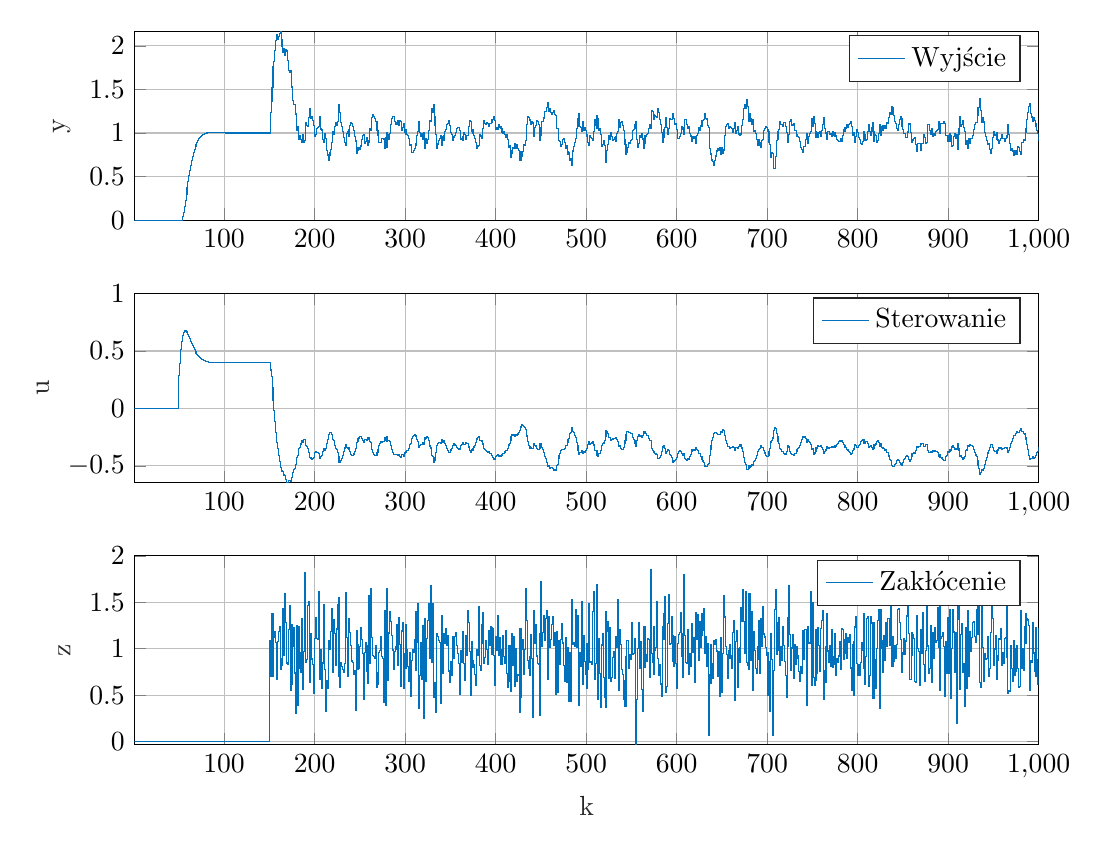
\begin{tikzpicture}

\begin{axis}[%
width=4.521in,
height=0.944in,
at={(0.758in,1.792in)},
scale only axis,
xmin=1,
xmax=1000,
ymin=-0.64468,
ymax=1,
ylabel style={font=\color{white!15!black}},
ylabel={u},
axis background/.style={fill=white},
xmajorgrids,
ymajorgrids,
legend style={legend cell align=left, align=left, draw=white!15!black}
]
\addplot[const plot, color=mycolor1] table[row sep=crcr] {%
1	0\\
2	0\\
3	0\\
4	0\\
5	0\\
6	0\\
7	0\\
8	0\\
9	0\\
10	0\\
11	0\\
12	0\\
13	0\\
14	0\\
15	0\\
16	0\\
17	0\\
18	0\\
19	0\\
20	0\\
21	0\\
22	0\\
23	0\\
24	0\\
25	0\\
26	0\\
27	0\\
28	0\\
29	0\\
30	0\\
31	0\\
32	0\\
33	0\\
34	0\\
35	0\\
36	0\\
37	0\\
38	0\\
39	0\\
40	0\\
41	0\\
42	0\\
43	0\\
44	0\\
45	0\\
46	0\\
47	0\\
48	0\\
49	0\\
50	0.28956\\
51	0.39251\\
52	0.5131\\
53	0.58007\\
54	0.63135\\
55	0.65951\\
56	0.67407\\
57	0.67664\\
58	0.67103\\
59	0.65931\\
60	0.64358\\
61	0.62529\\
62	0.60567\\
63	0.58562\\
64	0.56581\\
65	0.54674\\
66	0.52873\\
67	0.512\\
68	0.49669\\
69	0.48283\\
70	0.47042\\
71	0.45942\\
72	0.44977\\
73	0.44136\\
74	0.4341\\
75	0.42788\\
76	0.4226\\
77	0.41815\\
78	0.41444\\
79	0.41136\\
80	0.40884\\
81	0.4068\\
82	0.40516\\
83	0.40387\\
84	0.40286\\
85	0.40209\\
86	0.40151\\
87	0.4011\\
88	0.40081\\
89	0.40063\\
90	0.40052\\
91	0.40048\\
92	0.40048\\
93	0.40051\\
94	0.40057\\
95	0.40065\\
96	0.40073\\
97	0.40082\\
98	0.40091\\
99	0.401\\
100	0.40108\\
101	0.40116\\
102	0.40123\\
103	0.4013\\
104	0.40136\\
105	0.40142\\
106	0.40146\\
107	0.4015\\
108	0.40154\\
109	0.40157\\
110	0.4016\\
111	0.40162\\
112	0.40164\\
113	0.40166\\
114	0.40167\\
115	0.40168\\
116	0.40169\\
117	0.4017\\
118	0.4017\\
119	0.40171\\
120	0.40171\\
121	0.40171\\
122	0.40171\\
123	0.40172\\
124	0.40172\\
125	0.40172\\
126	0.40172\\
127	0.40172\\
128	0.40172\\
129	0.40172\\
130	0.40172\\
131	0.40172\\
132	0.40172\\
133	0.40171\\
134	0.40171\\
135	0.40171\\
136	0.40171\\
137	0.40171\\
138	0.40171\\
139	0.40171\\
140	0.40171\\
141	0.40171\\
142	0.40171\\
143	0.40171\\
144	0.40171\\
145	0.40171\\
146	0.40171\\
147	0.40171\\
148	0.40171\\
149	0.40171\\
150	0.40171\\
151	0.33435\\
152	0.27435\\
153	0.18472\\
154	0.068528\\
155	-0.014842\\
156	-0.11667\\
157	-0.21264\\
158	-0.29853\\
159	-0.34913\\
160	-0.40811\\
161	-0.46215\\
162	-0.51676\\
163	-0.53745\\
164	-0.54873\\
165	-0.5508\\
166	-0.57985\\
167	-0.58122\\
168	-0.62215\\
169	-0.64468\\
170	-0.64365\\
171	-0.62867\\
172	-0.62643\\
173	-0.63936\\
174	-0.6027\\
175	-0.60062\\
176	-0.55548\\
177	-0.53395\\
178	-0.52145\\
179	-0.48805\\
180	-0.42572\\
181	-0.41077\\
182	-0.34942\\
183	-0.34304\\
184	-0.3131\\
185	-0.30298\\
186	-0.28002\\
187	-0.29558\\
188	-0.27141\\
189	-0.27279\\
190	-0.32342\\
191	-0.3333\\
192	-0.34535\\
193	-0.38228\\
194	-0.4275\\
195	-0.42561\\
196	-0.43621\\
197	-0.44502\\
198	-0.43932\\
199	-0.42541\\
200	-0.38621\\
201	-0.37569\\
202	-0.38184\\
203	-0.38639\\
204	-0.39413\\
205	-0.43358\\
206	-0.43324\\
207	-0.41945\\
208	-0.41108\\
209	-0.37491\\
210	-0.35096\\
211	-0.36349\\
212	-0.34603\\
213	-0.30315\\
214	-0.26732\\
215	-0.2236\\
216	-0.21349\\
217	-0.20652\\
218	-0.21038\\
219	-0.23032\\
220	-0.27233\\
221	-0.28058\\
222	-0.3194\\
223	-0.34645\\
224	-0.35577\\
225	-0.38019\\
226	-0.41884\\
227	-0.46871\\
228	-0.47001\\
229	-0.45258\\
230	-0.43339\\
231	-0.40707\\
232	-0.37742\\
233	-0.34441\\
234	-0.31705\\
235	-0.33939\\
236	-0.34693\\
237	-0.3378\\
238	-0.35848\\
239	-0.37683\\
240	-0.39766\\
241	-0.40867\\
242	-0.40669\\
243	-0.39708\\
244	-0.37416\\
245	-0.34893\\
246	-0.29456\\
247	-0.28683\\
248	-0.25949\\
249	-0.25781\\
250	-0.24285\\
251	-0.24644\\
252	-0.26399\\
253	-0.28238\\
254	-0.29436\\
255	-0.27339\\
256	-0.27347\\
257	-0.2774\\
258	-0.26934\\
259	-0.25077\\
260	-0.2522\\
261	-0.28979\\
262	-0.29694\\
263	-0.35438\\
264	-0.38282\\
265	-0.40276\\
266	-0.41018\\
267	-0.4093\\
268	-0.4109\\
269	-0.38337\\
270	-0.35901\\
271	-0.32086\\
272	-0.30286\\
273	-0.2893\\
274	-0.29285\\
275	-0.28941\\
276	-0.28759\\
277	-0.25498\\
278	-0.27654\\
279	-0.24161\\
280	-0.28489\\
281	-0.28132\\
282	-0.27661\\
283	-0.29047\\
284	-0.32279\\
285	-0.35774\\
286	-0.38702\\
287	-0.40409\\
288	-0.40178\\
289	-0.40254\\
290	-0.39979\\
291	-0.39865\\
292	-0.41172\\
293	-0.40177\\
294	-0.42077\\
295	-0.42331\\
296	-0.40081\\
297	-0.40423\\
298	-0.41405\\
299	-0.38865\\
300	-0.37883\\
301	-0.3838\\
302	-0.36773\\
303	-0.36333\\
304	-0.34528\\
305	-0.31743\\
306	-0.3038\\
307	-0.26363\\
308	-0.24544\\
309	-0.23512\\
310	-0.23168\\
311	-0.24173\\
312	-0.23671\\
313	-0.27048\\
314	-0.28905\\
315	-0.33854\\
316	-0.32095\\
317	-0.31483\\
318	-0.31557\\
319	-0.2972\\
320	-0.312\\
321	-0.26871\\
322	-0.25031\\
323	-0.26022\\
324	-0.24333\\
325	-0.25529\\
326	-0.28041\\
327	-0.327\\
328	-0.34438\\
329	-0.4066\\
330	-0.41979\\
331	-0.46837\\
332	-0.44925\\
333	-0.43022\\
334	-0.38712\\
335	-0.32534\\
336	-0.30704\\
337	-0.29597\\
338	-0.29728\\
339	-0.30277\\
340	-0.27236\\
341	-0.29265\\
342	-0.27827\\
343	-0.29254\\
344	-0.30762\\
345	-0.32367\\
346	-0.34906\\
347	-0.36491\\
348	-0.38613\\
349	-0.38128\\
350	-0.36259\\
351	-0.3475\\
352	-0.32095\\
353	-0.31967\\
354	-0.30848\\
355	-0.31203\\
356	-0.32152\\
357	-0.33909\\
358	-0.35098\\
359	-0.35734\\
360	-0.35349\\
361	-0.32456\\
362	-0.31608\\
363	-0.29957\\
364	-0.30402\\
365	-0.31607\\
366	-0.31437\\
367	-0.29951\\
368	-0.30733\\
369	-0.30501\\
370	-0.33574\\
371	-0.36381\\
372	-0.37933\\
373	-0.35996\\
374	-0.36363\\
375	-0.34716\\
376	-0.33641\\
377	-0.31992\\
378	-0.2979\\
379	-0.26665\\
380	-0.25658\\
381	-0.24717\\
382	-0.277\\
383	-0.27759\\
384	-0.27724\\
385	-0.28642\\
386	-0.31015\\
387	-0.34777\\
388	-0.35791\\
389	-0.36663\\
390	-0.37825\\
391	-0.38357\\
392	-0.37732\\
393	-0.38897\\
394	-0.39203\\
395	-0.40992\\
396	-0.40993\\
397	-0.42632\\
398	-0.44114\\
399	-0.44106\\
400	-0.4163\\
401	-0.41389\\
402	-0.40184\\
403	-0.41703\\
404	-0.41008\\
405	-0.41623\\
406	-0.41145\\
407	-0.39762\\
408	-0.38909\\
409	-0.38908\\
410	-0.37956\\
411	-0.36537\\
412	-0.36971\\
413	-0.34927\\
414	-0.31889\\
415	-0.30807\\
416	-0.27744\\
417	-0.24138\\
418	-0.23061\\
419	-0.23508\\
420	-0.2298\\
421	-0.24525\\
422	-0.23035\\
423	-0.23815\\
424	-0.22255\\
425	-0.2112\\
426	-0.19588\\
427	-0.15603\\
428	-0.16613\\
429	-0.13836\\
430	-0.14652\\
431	-0.16132\\
432	-0.16435\\
433	-0.18198\\
434	-0.24064\\
435	-0.29111\\
436	-0.32079\\
437	-0.33482\\
438	-0.34576\\
439	-0.33813\\
440	-0.35156\\
441	-0.34929\\
442	-0.30894\\
443	-0.32612\\
444	-0.32726\\
445	-0.35177\\
446	-0.35666\\
447	-0.35687\\
448	-0.34918\\
449	-0.30449\\
450	-0.30378\\
451	-0.34006\\
452	-0.35498\\
453	-0.38166\\
454	-0.41561\\
455	-0.43677\\
456	-0.46885\\
457	-0.5041\\
458	-0.49521\\
459	-0.50548\\
460	-0.51922\\
461	-0.51808\\
462	-0.51829\\
463	-0.52484\\
464	-0.53803\\
465	-0.53501\\
466	-0.53748\\
467	-0.49544\\
468	-0.48549\\
469	-0.43327\\
470	-0.41463\\
471	-0.3908\\
472	-0.36452\\
473	-0.3546\\
474	-0.36017\\
475	-0.36152\\
476	-0.35091\\
477	-0.32565\\
478	-0.32308\\
479	-0.29392\\
480	-0.27052\\
481	-0.26036\\
482	-0.22091\\
483	-0.21085\\
484	-0.17023\\
485	-0.19893\\
486	-0.20869\\
487	-0.23292\\
488	-0.25217\\
489	-0.29726\\
490	-0.32127\\
491	-0.36592\\
492	-0.402\\
493	-0.38554\\
494	-0.38709\\
495	-0.3701\\
496	-0.39653\\
497	-0.37416\\
498	-0.38301\\
499	-0.37023\\
500	-0.35131\\
501	-0.34616\\
502	-0.31402\\
503	-0.2918\\
504	-0.31018\\
505	-0.30333\\
506	-0.30158\\
507	-0.29267\\
508	-0.31852\\
509	-0.36498\\
510	-0.36598\\
511	-0.36919\\
512	-0.41315\\
513	-0.41843\\
514	-0.39551\\
515	-0.39493\\
516	-0.36986\\
517	-0.32277\\
518	-0.30633\\
519	-0.30138\\
520	-0.27984\\
521	-0.24431\\
522	-0.19579\\
523	-0.2057\\
524	-0.21647\\
525	-0.2495\\
526	-0.24989\\
527	-0.28018\\
528	-0.27355\\
529	-0.26668\\
530	-0.26349\\
531	-0.26581\\
532	-0.25269\\
533	-0.26518\\
534	-0.27279\\
535	-0.28573\\
536	-0.3299\\
537	-0.32232\\
538	-0.34867\\
539	-0.35932\\
540	-0.35751\\
541	-0.34421\\
542	-0.30808\\
543	-0.2762\\
544	-0.22436\\
545	-0.20342\\
546	-0.19829\\
547	-0.20723\\
548	-0.20591\\
549	-0.21466\\
550	-0.22004\\
551	-0.25157\\
552	-0.26686\\
553	-0.284\\
554	-0.30452\\
555	-0.32707\\
556	-0.27952\\
557	-0.24387\\
558	-0.22855\\
559	-0.24119\\
560	-0.23629\\
561	-0.25188\\
562	-0.23601\\
563	-0.20307\\
564	-0.20174\\
565	-0.21835\\
566	-0.22072\\
567	-0.23242\\
568	-0.23777\\
569	-0.25846\\
570	-0.28061\\
571	-0.28107\\
572	-0.34655\\
573	-0.36608\\
574	-0.38261\\
575	-0.37638\\
576	-0.39475\\
577	-0.39704\\
578	-0.40295\\
579	-0.43564\\
580	-0.4379\\
581	-0.42677\\
582	-0.41043\\
583	-0.37697\\
584	-0.33042\\
585	-0.32452\\
586	-0.33601\\
587	-0.34637\\
588	-0.38858\\
589	-0.37397\\
590	-0.35613\\
591	-0.36412\\
592	-0.39785\\
593	-0.41122\\
594	-0.42518\\
595	-0.45114\\
596	-0.46666\\
597	-0.46428\\
598	-0.45027\\
599	-0.44786\\
600	-0.42824\\
601	-0.39111\\
602	-0.37551\\
603	-0.36847\\
604	-0.37188\\
605	-0.39403\\
606	-0.39405\\
607	-0.40772\\
608	-0.38939\\
609	-0.43483\\
610	-0.44749\\
611	-0.44926\\
612	-0.43744\\
613	-0.44189\\
614	-0.41754\\
615	-0.40415\\
616	-0.37816\\
617	-0.36234\\
618	-0.36606\\
619	-0.35916\\
620	-0.36474\\
621	-0.34108\\
622	-0.35975\\
623	-0.36406\\
624	-0.39245\\
625	-0.3921\\
626	-0.4153\\
627	-0.41902\\
628	-0.44583\\
629	-0.45797\\
630	-0.47464\\
631	-0.50198\\
632	-0.50245\\
633	-0.5092\\
634	-0.48996\\
635	-0.48054\\
636	-0.40654\\
637	-0.36004\\
638	-0.32675\\
639	-0.28131\\
640	-0.25141\\
641	-0.21499\\
642	-0.20854\\
643	-0.20738\\
644	-0.21919\\
645	-0.22861\\
646	-0.22334\\
647	-0.23057\\
648	-0.20742\\
649	-0.19886\\
650	-0.20673\\
651	-0.18683\\
652	-0.1909\\
653	-0.23245\\
654	-0.27562\\
655	-0.30785\\
656	-0.33014\\
657	-0.32926\\
658	-0.33726\\
659	-0.34455\\
660	-0.34429\\
661	-0.34349\\
662	-0.33211\\
663	-0.34219\\
664	-0.36298\\
665	-0.33813\\
666	-0.34358\\
667	-0.35208\\
668	-0.33181\\
669	-0.33093\\
670	-0.31824\\
671	-0.31794\\
672	-0.34508\\
673	-0.37325\\
674	-0.42884\\
675	-0.46791\\
676	-0.48597\\
677	-0.5335\\
678	-0.53383\\
679	-0.52611\\
680	-0.50007\\
681	-0.51821\\
682	-0.50519\\
683	-0.4893\\
684	-0.49728\\
685	-0.45885\\
686	-0.45436\\
687	-0.43444\\
688	-0.40824\\
689	-0.3746\\
690	-0.35649\\
691	-0.35921\\
692	-0.34683\\
693	-0.32693\\
694	-0.3385\\
695	-0.33848\\
696	-0.37015\\
697	-0.38802\\
698	-0.40751\\
699	-0.4155\\
700	-0.41498\\
701	-0.41066\\
702	-0.37408\\
703	-0.35139\\
704	-0.29208\\
705	-0.28084\\
706	-0.25766\\
707	-0.19534\\
708	-0.16498\\
709	-0.17567\\
710	-0.22016\\
711	-0.24117\\
712	-0.28448\\
713	-0.30734\\
714	-0.35032\\
715	-0.35932\\
716	-0.37609\\
717	-0.37561\\
718	-0.39423\\
719	-0.40033\\
720	-0.39673\\
721	-0.37783\\
722	-0.33781\\
723	-0.32329\\
724	-0.33059\\
725	-0.3724\\
726	-0.39598\\
727	-0.39806\\
728	-0.40366\\
729	-0.41321\\
730	-0.39482\\
731	-0.39272\\
732	-0.37447\\
733	-0.3608\\
734	-0.35301\\
735	-0.34282\\
736	-0.32335\\
737	-0.29492\\
738	-0.27306\\
739	-0.24709\\
740	-0.2516\\
741	-0.24489\\
742	-0.26409\\
743	-0.28666\\
744	-0.29735\\
745	-0.27316\\
746	-0.28927\\
747	-0.29601\\
748	-0.31052\\
749	-0.3581\\
750	-0.35319\\
751	-0.39673\\
752	-0.38804\\
753	-0.37233\\
754	-0.34377\\
755	-0.34511\\
756	-0.32274\\
757	-0.33289\\
758	-0.33377\\
759	-0.32398\\
760	-0.33754\\
761	-0.35921\\
762	-0.39545\\
763	-0.3773\\
764	-0.36665\\
765	-0.36019\\
766	-0.33311\\
767	-0.34842\\
768	-0.34498\\
769	-0.34026\\
770	-0.34141\\
771	-0.32974\\
772	-0.34167\\
773	-0.33069\\
774	-0.32717\\
775	-0.3356\\
776	-0.32856\\
777	-0.31331\\
778	-0.3031\\
779	-0.29033\\
780	-0.28325\\
781	-0.287\\
782	-0.27703\\
783	-0.29405\\
784	-0.3139\\
785	-0.32107\\
786	-0.33783\\
787	-0.34365\\
788	-0.36165\\
789	-0.36259\\
790	-0.37552\\
791	-0.38365\\
792	-0.39807\\
793	-0.39018\\
794	-0.36297\\
795	-0.3558\\
796	-0.35124\\
797	-0.3179\\
798	-0.32372\\
799	-0.33988\\
800	-0.33807\\
801	-0.32587\\
802	-0.31359\\
803	-0.29183\\
804	-0.27675\\
805	-0.27527\\
806	-0.27474\\
807	-0.30285\\
808	-0.30198\\
809	-0.28973\\
810	-0.28566\\
811	-0.30604\\
812	-0.3364\\
813	-0.32814\\
814	-0.31913\\
815	-0.33884\\
816	-0.36144\\
817	-0.3448\\
818	-0.31429\\
819	-0.321\\
820	-0.31021\\
821	-0.28623\\
822	-0.2812\\
823	-0.29737\\
824	-0.33156\\
825	-0.30923\\
826	-0.34147\\
827	-0.34728\\
828	-0.3436\\
829	-0.35118\\
830	-0.36233\\
831	-0.36073\\
832	-0.38125\\
833	-0.38763\\
834	-0.41427\\
835	-0.44158\\
836	-0.45516\\
837	-0.49356\\
838	-0.50975\\
839	-0.50464\\
840	-0.50687\\
841	-0.48857\\
842	-0.47807\\
843	-0.45622\\
844	-0.44344\\
845	-0.45365\\
846	-0.47342\\
847	-0.49203\\
848	-0.50026\\
849	-0.4825\\
850	-0.46865\\
851	-0.44775\\
852	-0.43782\\
853	-0.41891\\
854	-0.4106\\
855	-0.42013\\
856	-0.44834\\
857	-0.46273\\
858	-0.44704\\
859	-0.41936\\
860	-0.3974\\
861	-0.3901\\
862	-0.38814\\
863	-0.38928\\
864	-0.36432\\
865	-0.33306\\
866	-0.33895\\
867	-0.33227\\
868	-0.33042\\
869	-0.30424\\
870	-0.31086\\
871	-0.30815\\
872	-0.3082\\
873	-0.334\\
874	-0.33209\\
875	-0.31781\\
876	-0.31388\\
877	-0.36733\\
878	-0.38332\\
879	-0.38505\\
880	-0.37478\\
881	-0.3759\\
882	-0.38748\\
883	-0.36686\\
884	-0.37388\\
885	-0.36274\\
886	-0.37515\\
887	-0.37887\\
888	-0.38736\\
889	-0.416\\
890	-0.42441\\
891	-0.40286\\
892	-0.42806\\
893	-0.43198\\
894	-0.44355\\
895	-0.45354\\
896	-0.455\\
897	-0.42029\\
898	-0.4103\\
899	-0.37713\\
900	-0.3832\\
901	-0.35687\\
902	-0.37596\\
903	-0.36782\\
904	-0.33605\\
905	-0.32518\\
906	-0.34058\\
907	-0.35372\\
908	-0.34602\\
909	-0.35837\\
910	-0.31011\\
911	-0.34638\\
912	-0.36377\\
913	-0.41834\\
914	-0.40879\\
915	-0.42746\\
916	-0.44287\\
917	-0.43184\\
918	-0.41813\\
919	-0.36828\\
920	-0.36228\\
921	-0.3196\\
922	-0.3323\\
923	-0.33048\\
924	-0.31616\\
925	-0.32485\\
926	-0.32349\\
927	-0.33486\\
928	-0.35658\\
929	-0.38449\\
930	-0.40557\\
931	-0.42085\\
932	-0.45376\\
933	-0.4983\\
934	-0.52208\\
935	-0.57436\\
936	-0.5609\\
937	-0.53313\\
938	-0.538\\
939	-0.52106\\
940	-0.48495\\
941	-0.45745\\
942	-0.42498\\
943	-0.39571\\
944	-0.38188\\
945	-0.36942\\
946	-0.34092\\
947	-0.31545\\
948	-0.31168\\
949	-0.34083\\
950	-0.36857\\
951	-0.37205\\
952	-0.37872\\
953	-0.38842\\
954	-0.37007\\
955	-0.36134\\
956	-0.34466\\
957	-0.34371\\
958	-0.34481\\
959	-0.3585\\
960	-0.351\\
961	-0.34962\\
962	-0.33745\\
963	-0.34111\\
964	-0.34674\\
965	-0.34385\\
966	-0.38548\\
967	-0.36569\\
968	-0.34233\\
969	-0.30176\\
970	-0.28816\\
971	-0.26375\\
972	-0.23615\\
973	-0.23357\\
974	-0.21477\\
975	-0.20212\\
976	-0.2026\\
977	-0.21114\\
978	-0.20984\\
979	-0.1954\\
980	-0.17616\\
981	-0.20325\\
982	-0.20349\\
983	-0.22176\\
984	-0.22241\\
985	-0.25189\\
986	-0.27236\\
987	-0.3166\\
988	-0.36009\\
989	-0.40627\\
990	-0.44644\\
991	-0.43974\\
992	-0.43785\\
993	-0.4231\\
994	-0.43259\\
995	-0.42518\\
996	-0.40715\\
997	-0.41187\\
998	-0.38723\\
999	-0.373\\
1000	-0.33784\\
};
\addlegendentry{Sterowanie}

\end{axis}

\begin{axis}[%
width=4.521in,
height=0.944in,
at={(0.758in,3.103in)},
scale only axis,
xmin=1,
xmax=1000,
ymin=0,
ymax=2.1649,
ylabel style={font=\color{white!15!black}},
ylabel={y},
axis background/.style={fill=white},
xmajorgrids,
ymajorgrids,
legend style={legend cell align=left, align=left, draw=white!15!black}
]
\addplot[const plot, color=mycolor1] table[row sep=crcr] {%
1	0\\
2	0\\
3	0\\
4	0\\
5	0\\
6	0\\
7	0\\
8	0\\
9	0\\
10	0\\
11	0\\
12	0\\
13	0\\
14	0\\
15	0\\
16	0\\
17	0\\
18	0\\
19	0\\
20	0\\
21	0\\
22	0\\
23	0\\
24	0\\
25	0\\
26	0\\
27	0\\
28	0\\
29	0\\
30	0\\
31	0\\
32	0\\
33	0\\
34	0\\
35	0\\
36	0\\
37	0\\
38	0\\
39	0\\
40	0\\
41	0\\
42	0\\
43	0\\
44	0\\
45	0\\
46	0\\
47	0\\
48	0\\
49	0\\
50	0\\
51	0\\
52	0\\
53	0\\
54	0.039119\\
55	0.090032\\
56	0.15448\\
57	0.22449\\
58	0.29764\\
59	0.37063\\
60	0.44164\\
61	0.50914\\
62	0.57223\\
63	0.63032\\
64	0.68313\\
65	0.73061\\
66	0.77286\\
67	0.81011\\
68	0.84266\\
69	0.87086\\
70	0.8951\\
71	0.91576\\
72	0.93322\\
73	0.94786\\
74	0.96003\\
75	0.97004\\
76	0.97821\\
77	0.98479\\
78	0.99003\\
79	0.99414\\
80	0.99731\\
81	0.99971\\
82	1.0015\\
83	1.0027\\
84	1.0036\\
85	1.0041\\
86	1.0043\\
87	1.0044\\
88	1.0043\\
89	1.0042\\
90	1.0039\\
91	1.0036\\
92	1.0033\\
93	1.003\\
94	1.0027\\
95	1.0024\\
96	1.0021\\
97	1.0018\\
98	1.0016\\
99	1.0013\\
100	1.0011\\
101	1.001\\
102	1.0008\\
103	1.0007\\
104	1.0005\\
105	1.0004\\
106	1.0003\\
107	1.0003\\
108	1.0002\\
109	1.0002\\
110	1.0001\\
111	1.0001\\
112	1.0001\\
113	1\\
114	1\\
115	1\\
116	1\\
117	0.99999\\
118	0.99998\\
119	0.99998\\
120	0.99998\\
121	0.99998\\
122	0.99998\\
123	0.99998\\
124	0.99998\\
125	0.99998\\
126	0.99998\\
127	0.99998\\
128	0.99998\\
129	0.99998\\
130	0.99998\\
131	0.99998\\
132	0.99999\\
133	0.99999\\
134	0.99999\\
135	0.99999\\
136	0.99999\\
137	0.99999\\
138	0.99999\\
139	0.99999\\
140	0.99999\\
141	0.99999\\
142	0.99999\\
143	0.99999\\
144	0.99999\\
145	0.99999\\
146	0.99999\\
147	0.99999\\
148	0.99999\\
149	0.99999\\
150	0.99999\\
151	1.2326\\
152	1.3571\\
153	1.5255\\
154	1.7613\\
155	1.8161\\
156	1.9466\\
157	2.0629\\
158	2.1236\\
159	2.0773\\
160	2.1072\\
161	2.1395\\
162	2.1649\\
163	2.0767\\
164	1.9949\\
165	1.9255\\
166	1.9664\\
167	1.8881\\
168	1.9545\\
169	1.9407\\
170	1.8267\\
171	1.7169\\
172	1.6898\\
173	1.7123\\
174	1.5335\\
175	1.5238\\
176	1.3757\\
177	1.3247\\
178	1.3258\\
179	1.2186\\
180	1.0342\\
181	1.0733\\
182	0.92334\\
183	0.97399\\
184	0.9306\\
185	0.92786\\
186	0.88846\\
187	0.97697\\
188	0.89735\\
189	0.916\\
190	1.1173\\
191	1.0879\\
192	1.07\\
193	1.1793\\
194	1.278\\
195	1.1784\\
196	1.1725\\
197	1.1903\\
198	1.1415\\
199	1.0854\\
200	0.96608\\
201	0.98384\\
202	1.0496\\
203	1.0601\\
204	1.072\\
205	1.1931\\
206	1.1342\\
207	1.0459\\
208	1.0345\\
209	0.92854\\
210	0.89286\\
211	0.99757\\
212	0.94056\\
213	0.79962\\
214	0.74842\\
215	0.68377\\
216	0.73727\\
217	0.77162\\
218	0.80758\\
219	0.88762\\
220	1.0137\\
221	0.9807\\
222	1.0729\\
223	1.1204\\
224	1.0848\\
225	1.1363\\
226	1.2324\\
227	1.3316\\
228	1.2355\\
229	1.1225\\
230	1.0733\\
231	1.0139\\
232	0.95273\\
233	0.89272\\
234	0.86097\\
235	0.99922\\
236	1.0217\\
237	0.95775\\
238	1.0373\\
239	1.0862\\
240	1.1149\\
241	1.1117\\
242	1.0714\\
243	1.0295\\
244	0.96204\\
245	0.90902\\
246	0.77132\\
247	0.83273\\
248	0.79988\\
249	0.83285\\
250	0.81504\\
251	0.85082\\
252	0.92875\\
253	0.97267\\
254	0.98138\\
255	0.88371\\
256	0.90404\\
257	0.94283\\
258	0.9111\\
259	0.85672\\
260	0.89639\\
261	1.0456\\
262	1.025\\
263	1.1816\\
264	1.209\\
265	1.1873\\
266	1.1647\\
267	1.1313\\
268	1.1268\\
269	1.025\\
270	0.96662\\
271	0.88653\\
272	0.88797\\
273	0.89626\\
274	0.93895\\
275	0.93617\\
276	0.93199\\
277	0.82846\\
278	0.94728\\
279	0.83555\\
280	1.0069\\
281	0.98282\\
282	0.92837\\
283	0.99402\\
284	1.0952\\
285	1.1642\\
286	1.1935\\
287	1.1851\\
288	1.1282\\
289	1.1152\\
290	1.103\\
291	1.0954\\
292	1.1391\\
293	1.0842\\
294	1.1439\\
295	1.1357\\
296	1.0299\\
297	1.0638\\
298	1.1109\\
299	1.0009\\
300	0.98516\\
301	1.037\\
302	0.97956\\
303	0.97648\\
304	0.93484\\
305	0.86268\\
306	0.8673\\
307	0.77207\\
308	0.77165\\
309	0.80083\\
310	0.82109\\
311	0.87572\\
312	0.85629\\
313	0.97659\\
314	1.0126\\
315	1.1331\\
316	1.0018\\
317	0.95785\\
318	0.99125\\
319	0.93052\\
320	1.003\\
321	0.85427\\
322	0.82815\\
323	0.93096\\
324	0.87642\\
325	0.9308\\
326	1.0251\\
327	1.1456\\
328	1.1288\\
329	1.2809\\
330	1.2375\\
331	1.3262\\
332	1.1887\\
333	1.0916\\
334	0.98105\\
335	0.82775\\
336	0.87358\\
337	0.90982\\
338	0.93853\\
339	0.96674\\
340	0.85515\\
341	0.96008\\
342	0.91896\\
343	0.96562\\
344	1.0201\\
345	1.0443\\
346	1.1015\\
347	1.1122\\
348	1.1427\\
349	1.0856\\
350	1.0049\\
351	0.97914\\
352	0.92008\\
353	0.9584\\
354	0.94471\\
355	0.96915\\
356	1.0096\\
357	1.0552\\
358	1.0671\\
359	1.0589\\
360	1.0277\\
361	0.92626\\
362	0.93535\\
363	0.91563\\
364	0.9563\\
365	1.009\\
366	0.984\\
367	0.92528\\
368	0.97495\\
369	0.97303\\
370	1.0741\\
371	1.1381\\
372	1.1277\\
373	1.0171\\
374	1.0392\\
375	0.99548\\
376	0.9699\\
377	0.94078\\
378	0.89236\\
379	0.82625\\
380	0.8506\\
381	0.86123\\
382	0.98621\\
383	0.96488\\
384	0.93741\\
385	0.97638\\
386	1.0504\\
387	1.1448\\
388	1.1132\\
389	1.0967\\
390	1.1186\\
391	1.1122\\
392	1.0699\\
393	1.1097\\
394	1.1085\\
395	1.1501\\
396	1.1222\\
397	1.1569\\
398	1.1849\\
399	1.1447\\
400	1.0406\\
401	1.0579\\
402	1.0375\\
403	1.0992\\
404	1.0643\\
405	1.0743\\
406	1.0555\\
407	1.0034\\
408	0.99315\\
409	1.0139\\
410	0.9859\\
411	0.94642\\
412	0.98743\\
413	0.92424\\
414	0.83897\\
415	0.86051\\
416	0.79756\\
417	0.72129\\
418	0.76227\\
419	0.82941\\
420	0.82039\\
421	0.88357\\
422	0.82761\\
423	0.86508\\
424	0.82563\\
425	0.80325\\
426	0.7876\\
427	0.68532\\
428	0.79072\\
429	0.72872\\
430	0.7862\\
431	0.86626\\
432	0.85763\\
433	0.91114\\
434	1.0995\\
435	1.1923\\
436	1.1826\\
437	1.1537\\
438	1.1492\\
439	1.0951\\
440	1.1366\\
441	1.1155\\
442	0.95944\\
443	1.0668\\
444	1.0844\\
445	1.1428\\
446	1.1277\\
447	1.095\\
448	1.0621\\
449	0.91285\\
450	0.96843\\
451	1.1345\\
452	1.1356\\
453	1.1728\\
454	1.2446\\
455	1.2476\\
456	1.2967\\
457	1.3549\\
458	1.2428\\
459	1.2477\\
460	1.2836\\
461	1.2397\\
462	1.2179\\
463	1.2314\\
464	1.2572\\
465	1.2133\\
466	1.2027\\
467	1.0484\\
468	1.0526\\
469	0.91708\\
470	0.91461\\
471	0.90099\\
472	0.84974\\
473	0.86945\\
474	0.92599\\
475	0.93405\\
476	0.8933\\
477	0.82243\\
478	0.859\\
479	0.78944\\
480	0.74924\\
481	0.77741\\
482	0.68049\\
483	0.70993\\
484	0.62919\\
485	0.79422\\
486	0.84368\\
487	0.89489\\
488	0.93712\\
489	1.0562\\
490	1.0755\\
491	1.1635\\
492	1.2177\\
493	1.0754\\
494	1.0681\\
495	1.0235\\
496	1.1276\\
497	1.0311\\
498	1.0577\\
499	1.0245\\
500	0.96034\\
501	0.97684\\
502	0.8874\\
503	0.85221\\
504	0.97442\\
505	0.94825\\
506	0.93295\\
507	0.91615\\
508	1.0199\\
509	1.16\\
510	1.0824\\
511	1.0505\\
512	1.2017\\
513	1.1606\\
514	1.0289\\
515	1.0505\\
516	0.98269\\
517	0.8445\\
518	0.86716\\
519	0.91245\\
520	0.8561\\
521	0.76576\\
522	0.66616\\
523	0.79736\\
524	0.87317\\
525	0.96763\\
526	0.92819\\
527	1.0086\\
528	0.95786\\
529	0.91671\\
530	0.9273\\
531	0.94776\\
532	0.90475\\
533	0.96423\\
534	0.9913\\
535	1.0158\\
536	1.149\\
537	1.0584\\
538	1.117\\
539	1.1327\\
540	1.0839\\
541	1.0295\\
542	0.91998\\
543	0.86331\\
544	0.75488\\
545	0.77302\\
546	0.83078\\
547	0.88758\\
548	0.88152\\
549	0.91096\\
550	0.92761\\
551	1.0269\\
552	1.0419\\
553	1.0559\\
554	1.0967\\
555	1.1349\\
556	0.92418\\
557	0.83756\\
558	0.87555\\
559	0.96685\\
560	0.94724\\
561	0.99584\\
562	0.93109\\
563	0.82316\\
564	0.87851\\
565	0.97076\\
566	0.95994\\
567	0.98525\\
568	0.99249\\
569	1.0488\\
570	1.098\\
571	1.0537\\
572	1.2598\\
573	1.2476\\
574	1.2133\\
575	1.1547\\
576	1.2043\\
577	1.1897\\
578	1.1804\\
579	1.2779\\
580	1.2317\\
581	1.1503\\
582	1.0998\\
583	1.0059\\
584	0.89255\\
585	0.95369\\
586	1.0385\\
587	1.0591\\
588	1.18\\
589	1.0683\\
590	0.98238\\
591	1.048\\
592	1.1673\\
593	1.1599\\
594	1.1569\\
595	1.2163\\
596	1.2206\\
597	1.1633\\
598	1.0984\\
599	1.1035\\
600	1.0447\\
601	0.93463\\
602	0.9399\\
603	0.96514\\
604	0.99483\\
605	1.0721\\
606	1.0413\\
607	1.0672\\
608	0.98896\\
609	1.1535\\
610	1.1596\\
611	1.1014\\
612	1.0482\\
613	1.0734\\
614	0.99132\\
615	0.96539\\
616	0.9135\\
617	0.8991\\
618	0.95497\\
619	0.94012\\
620	0.9644\\
621	0.88536\\
622	0.97485\\
623	0.99325\\
624	1.0675\\
625	1.0318\\
626	1.0862\\
627	1.0743\\
628	1.1385\\
629	1.1449\\
630	1.1589\\
631	1.2203\\
632	1.1685\\
633	1.1603\\
634	1.0814\\
635	1.0586\\
636	0.82753\\
637	0.75902\\
638	0.76942\\
639	0.69057\\
640	0.67443\\
641	0.63293\\
642	0.68868\\
643	0.7363\\
644	0.79333\\
645	0.82494\\
646	0.79586\\
647	0.83067\\
648	0.7583\\
649	0.75887\\
650	0.8294\\
651	0.76618\\
652	0.80553\\
653	0.97394\\
654	1.0749\\
655	1.1012\\
656	1.1068\\
657	1.0522\\
658	1.0627\\
659	1.0799\\
660	1.06\\
661	1.0489\\
662	1.009\\
663	1.0558\\
664	1.124\\
665	0.99943\\
666	1.0272\\
667	1.0741\\
668	0.98311\\
669	0.9953\\
670	0.97167\\
671	0.98341\\
672	1.0894\\
673	1.1522\\
674	1.2826\\
675	1.3232\\
676	1.2823\\
677	1.3854\\
678	1.3055\\
679	1.2226\\
680	1.1347\\
681	1.224\\
682	1.1699\\
683	1.0999\\
684	1.1524\\
685	1.0154\\
686	1.0298\\
687	0.99903\\
688	0.92811\\
689	0.86\\
690	0.86043\\
691	0.92232\\
692	0.89234\\
693	0.83748\\
694	0.91823\\
695	0.9264\\
696	1.0269\\
697	1.0558\\
698	1.0736\\
699	1.0654\\
700	1.037\\
701	1.0162\\
702	0.89504\\
703	0.86415\\
704	0.72195\\
705	0.77499\\
706	0.76802\\
707	0.59137\\
708	0.59243\\
709	0.73481\\
710	0.91002\\
711	0.92764\\
712	1.0215\\
713	1.0417\\
714	1.1288\\
715	1.0939\\
716	1.1026\\
717	1.0758\\
718	1.123\\
719	1.1207\\
720	1.0789\\
721	1.0103\\
722	0.89517\\
723	0.90853\\
724	0.98651\\
725	1.1314\\
726	1.1538\\
727	1.0923\\
728	1.0893\\
729	1.113\\
730	1.0288\\
731	1.0314\\
732	0.9864\\
733	0.95827\\
734	0.96367\\
735	0.9481\\
736	0.89931\\
737	0.83475\\
738	0.81359\\
739	0.77915\\
740	0.84914\\
741	0.84938\\
742	0.92337\\
743	0.99199\\
744	0.98801\\
745	0.87671\\
746	0.95786\\
747	0.98941\\
748	1.0156\\
749	1.1602\\
750	1.0732\\
751	1.1848\\
752	1.1102\\
753	1.02\\
754	0.95019\\
755	0.99988\\
756	0.9443\\
757	1.0006\\
758	1.0129\\
759	0.96555\\
760	1.025\\
761	1.0931\\
762	1.1774\\
763	1.0501\\
764	1.0006\\
765	1.0102\\
766	0.92977\\
767	1.0189\\
768	1.013\\
769	0.98242\\
770	0.99738\\
771	0.95972\\
772	1.0136\\
773	0.97293\\
774	0.96159\\
775	1.0078\\
776	0.97583\\
777	0.92392\\
778	0.916\\
779	0.89956\\
780	0.90078\\
781	0.93632\\
782	0.90595\\
783	0.97597\\
784	1.0374\\
785	1.0231\\
786	1.0571\\
787	1.053\\
788	1.0925\\
789	1.0691\\
790	1.094\\
791	1.1051\\
792	1.1295\\
793	1.0748\\
794	0.97338\\
795	0.98731\\
796	1.0026\\
797	0.89469\\
798	0.95827\\
799	1.039\\
800	1.0042\\
801	0.95029\\
802	0.92703\\
803	0.8791\\
804	0.86542\\
805	0.9008\\
806	0.91623\\
807	1.0177\\
808	0.9847\\
809	0.9193\\
810	0.92694\\
811	1.0162\\
812	1.1009\\
813	1.0168\\
814	0.96938\\
815	1.0599\\
816	1.121\\
817	1.0149\\
818	0.90878\\
819	0.98634\\
820	0.9675\\
821	0.88761\\
822	0.91171\\
823	0.99726\\
824	1.0998\\
825	0.96679\\
826	1.0752\\
827	1.082\\
828	1.0273\\
829	1.0551\\
830	1.0868\\
831	1.0578\\
832	1.1184\\
833	1.1155\\
834	1.1763\\
835	1.2305\\
836	1.2139\\
837	1.3003\\
838	1.2917\\
839	1.2094\\
840	1.202\\
841	1.1322\\
842	1.1052\\
843	1.0513\\
844	1.0339\\
845	1.0985\\
846	1.1591\\
847	1.1834\\
848	1.1665\\
849	1.0738\\
850	1.0357\\
851	0.99277\\
852	0.99042\\
853	0.95247\\
854	0.95194\\
855	1.0114\\
856	1.1031\\
857	1.1083\\
858	1.0097\\
859	0.92101\\
860	0.89403\\
861	0.91968\\
862	0.94047\\
863	0.95314\\
864	0.86902\\
865	0.79285\\
866	0.87911\\
867	0.88061\\
868	0.87824\\
869	0.80303\\
870	0.86455\\
871	0.87846\\
872	0.87866\\
873	0.97756\\
874	0.94494\\
875	0.87787\\
876	0.89098\\
877	1.0979\\
878	1.0937\\
879	1.0304\\
880	0.98459\\
881	1.0006\\
882	1.0487\\
883	0.96042\\
884	0.99825\\
885	0.9723\\
886	1.0193\\
887	1.0289\\
888	1.0404\\
889	1.1267\\
890	1.112\\
891	0.99872\\
892	1.1047\\
893	1.1065\\
894	1.1115\\
895	1.1278\\
896	1.1059\\
897	0.97152\\
898	0.97475\\
899	0.90275\\
900	0.9676\\
901	0.89998\\
902	0.9889\\
903	0.96552\\
904	0.84577\\
905	0.85942\\
906	0.9584\\
907	0.99529\\
908	0.94024\\
909	0.98467\\
910	0.81454\\
911	0.98812\\
912	1.0553\\
913	1.1842\\
914	1.074\\
915	1.0987\\
916	1.1429\\
917	1.0633\\
918	1.0129\\
919	0.86618\\
920	0.91518\\
921	0.82065\\
922	0.91722\\
923	0.939\\
924	0.8778\\
925	0.93264\\
926	0.93492\\
927	0.96952\\
928	1.0367\\
929	1.0983\\
930	1.1192\\
931	1.1219\\
932	1.1982\\
933	1.2964\\
934	1.2892\\
935	1.3946\\
936	1.2574\\
937	1.1187\\
938	1.1769\\
939	1.1264\\
940	1.0044\\
941	0.96235\\
942	0.91036\\
943	0.86726\\
944	0.88205\\
945	0.88121\\
946	0.81039\\
947	0.77145\\
948	0.82074\\
949	0.95367\\
950	1.0215\\
951	0.9773\\
952	0.97741\\
953	1.0059\\
954	0.92671\\
955	0.91197\\
956	0.88569\\
957	0.91119\\
958	0.93432\\
959	0.98261\\
960	0.94228\\
961	0.93655\\
962	0.90786\\
963	0.93838\\
964	0.96788\\
965	0.94891\\
966	1.094\\
967	0.98055\\
968	0.88447\\
969	0.798\\
970	0.82209\\
971	0.79421\\
972	0.74194\\
973	0.79541\\
974	0.76527\\
975	0.75242\\
976	0.79689\\
977	0.84552\\
978	0.83838\\
979	0.79118\\
980	0.75339\\
981	0.89288\\
982	0.88632\\
983	0.92889\\
984	0.91946\\
985	1.0089\\
986	1.0503\\
987	1.1532\\
988	1.235\\
989	1.3003\\
990	1.3424\\
991	1.2241\\
992	1.1833\\
993	1.1357\\
994	1.1772\\
995	1.1449\\
996	1.0721\\
997	1.1111\\
998	1.0299\\
999	0.9982\\
1000	0.91404\\
};
\addlegendentry{Wyjście}

\end{axis}

\begin{axis}[%
width=4.521in,
height=0.944in,
at={(0.758in,0.481in)},
scale only axis,
xmin=1,
xmax=1000,
xlabel style={font=\color{white!15!black}},
xlabel={k},
ymin=-0.033221,
ymax=2,
ylabel style={font=\color{white!15!black}},
ylabel={z},
axis background/.style={fill=white},
xmajorgrids,
ymajorgrids,
legend style={legend cell align=left, align=left, draw=white!15!black}
]
\addplot[const plot, color=mycolor1] table[row sep=crcr] {%
1	0\\
2	0\\
3	0\\
4	0\\
5	0\\
6	0\\
7	0\\
8	0\\
9	0\\
10	0\\
11	0\\
12	0\\
13	0\\
14	0\\
15	0\\
16	0\\
17	0\\
18	0\\
19	0\\
20	0\\
21	0\\
22	0\\
23	0\\
24	0\\
25	0\\
26	0\\
27	0\\
28	0\\
29	0\\
30	0\\
31	0\\
32	0\\
33	0\\
34	0\\
35	0\\
36	0\\
37	0\\
38	0\\
39	0\\
40	0\\
41	0\\
42	0\\
43	0\\
44	0\\
45	0\\
46	0\\
47	0\\
48	0\\
49	0\\
50	0\\
51	0\\
52	0\\
53	0\\
54	0\\
55	0\\
56	0\\
57	0\\
58	0\\
59	0\\
60	0\\
61	0\\
62	0\\
63	0\\
64	0\\
65	0\\
66	0\\
67	0\\
68	0\\
69	0\\
70	0\\
71	0\\
72	0\\
73	0\\
74	0\\
75	0\\
76	0\\
77	0\\
78	0\\
79	0\\
80	0\\
81	0\\
82	0\\
83	0\\
84	0\\
85	0\\
86	0\\
87	0\\
88	0\\
89	0\\
90	0\\
91	0\\
92	0\\
93	0\\
94	0\\
95	0\\
96	0\\
97	0\\
98	0\\
99	0\\
100	0\\
101	0\\
102	0\\
103	0\\
104	0\\
105	0\\
106	0\\
107	0\\
108	0\\
109	0\\
110	0\\
111	0\\
112	0\\
113	0\\
114	0\\
115	0\\
116	0\\
117	0\\
118	0\\
119	0\\
120	0\\
121	0\\
122	0\\
123	0\\
124	0\\
125	0\\
126	0\\
127	0\\
128	0\\
129	0\\
130	0\\
131	0\\
132	0\\
133	0\\
134	0\\
135	0\\
136	0\\
137	0\\
138	0\\
139	0\\
140	0\\
141	0\\
142	0\\
143	0\\
144	0\\
145	0\\
146	0\\
147	0\\
148	0\\
149	0\\
150	1.0909\\
151	0.70634\\
152	0.97762\\
153	1.3821\\
154	0.70079\\
155	1.1245\\
156	1.1887\\
157	1.0701\\
158	0.66454\\
159	1.0762\\
160	1.1809\\
161	1.2398\\
162	0.77423\\
163	0.8176\\
164	0.89016\\
165	1.4294\\
166	0.93024\\
167	1.599\\
168	1.2819\\
169	0.84596\\
170	0.82801\\
171	1.205\\
172	1.4593\\
173	0.54706\\
174	1.2561\\
175	0.61859\\
176	1.0216\\
177	1.2319\\
178	0.73801\\
179	0.30477\\
180	1.2527\\
181	0.38864\\
182	1.238\\
183	0.79111\\
184	0.95374\\
185	0.74504\\
186	1.3211\\
187	0.56108\\
188	0.97327\\
189	1.8244\\
190	0.85644\\
191	0.87921\\
192	1.4654\\
193	1.5036\\
194	0.63236\\
195	1.0275\\
196	1.1602\\
197	0.88858\\
198	0.83109\\
199	0.51563\\
200	1.1052\\
201	1.3398\\
202	1.1104\\
203	1.1003\\
204	1.6131\\
205	0.83748\\
206	0.67281\\
207	0.99251\\
208	0.56959\\
209	0.84591\\
210	1.4792\\
211	0.77258\\
212	0.32758\\
213	0.65909\\
214	0.57623\\
215	1.0848\\
216	0.99507\\
217	0.99548\\
218	1.1898\\
219	1.4364\\
220	0.747\\
221	1.3142\\
222	1.161\\
223	0.81933\\
224	1.212\\
225	1.4716\\
226	1.5535\\
227	0.69683\\
228	0.58373\\
229	0.8503\\
230	0.81158\\
231	0.77755\\
232	0.74472\\
233	0.83735\\
234	1.6042\\
235	1.1171\\
236	0.70338\\
237	1.3248\\
238	1.2354\\
239	1.1707\\
240	1.0297\\
241	0.86713\\
242	0.84993\\
243	0.7218\\
244	0.76265\\
245	0.3383\\
246	1.1951\\
247	0.77208\\
248	1.0477\\
249	0.79189\\
250	1.0263\\
251	1.2227\\
252	1.0996\\
253	0.94465\\
254	0.44882\\
255	0.95841\\
256	1.0647\\
257	0.76013\\
258	0.62265\\
259	1.0331\\
260	1.5684\\
261	0.84352\\
262	1.6504\\
263	1.1252\\
264	0.93105\\
265	0.91943\\
266	0.89267\\
267	1.0303\\
268	0.58689\\
269	0.74503\\
270	0.61524\\
271	0.95958\\
272	0.97803\\
273	1.1301\\
274	0.91601\\
275	0.89597\\
276	0.41809\\
277	1.4068\\
278	0.38464\\
279	1.6505\\
280	0.80224\\
281	0.65818\\
282	1.1689\\
283	1.3947\\
284	1.2937\\
285	1.1396\\
286	0.98557\\
287	0.77377\\
288	0.97237\\
289	0.98958\\
290	1.0181\\
291	1.2565\\
292	0.82086\\
293	1.3304\\
294	1.045\\
295	0.59384\\
296	1.19\\
297	1.2835\\
298	0.57625\\
299	0.94915\\
300	1.2617\\
301	0.78422\\
302	0.99503\\
303	0.80738\\
304	0.64615\\
305	0.95877\\
306	0.49029\\
307	0.87323\\
308	0.99351\\
309	0.95666\\
310	1.1009\\
311	0.76738\\
312	1.4019\\
313	1.0638\\
314	1.481\\
315	0.35739\\
316	0.71549\\
317	1.065\\
318	0.67133\\
319	1.2537\\
320	0.25043\\
321	0.74743\\
322	1.3265\\
323	0.65115\\
324	1.1056\\
325	1.3077\\
326	1.4845\\
327	0.89089\\
328	1.6798\\
329	0.85646\\
330	1.4822\\
331	0.48026\\
332	0.63815\\
333	0.53583\\
334	0.31214\\
335	1.1587\\
336	1.1304\\
337	1.0904\\
338	1.0658\\
339	0.41298\\
340	1.3614\\
341	0.73106\\
342	1.1231\\
343	1.164\\
344	1.061\\
345	1.2184\\
346	1.0378\\
347	1.1446\\
348	0.75938\\
349	0.63505\\
350	0.86113\\
351	0.70648\\
352	1.1312\\
353	0.89759\\
354	1.0607\\
355	1.1322\\
356	1.1768\\
357	1.035\\
358	0.94798\\
359	0.84152\\
360	0.50658\\
361	0.97929\\
362	0.85375\\
363	1.1251\\
364	1.1855\\
365	0.8428\\
366	0.66064\\
367	1.1396\\
368	0.93046\\
369	1.4108\\
370	1.2805\\
371	0.96871\\
372	0.49183\\
373	1.074\\
374	0.79564\\
375	0.86886\\
376	0.82843\\
377	0.72605\\
378	0.60835\\
379	0.99146\\
380	0.9296\\
381	1.4569\\
382	0.81545\\
383	0.7667\\
384	1.0553\\
385	1.2563\\
386	1.3894\\
387	0.84642\\
388	0.90518\\
389	1.091\\
390	0.99291\\
391	0.82965\\
392	1.1993\\
393	1.0369\\
394	1.2428\\
395	0.93741\\
396	1.2249\\
397	1.2163\\
398	0.925\\
399	0.60678\\
400	1.1343\\
401	0.97891\\
402	1.357\\
403	0.92372\\
404	1.1165\\
405	0.98136\\
406	0.82601\\
407	0.99273\\
408	1.1379\\
409	0.91906\\
410	0.84304\\
411	1.1951\\
412	0.72852\\
413	0.58615\\
414	1.0332\\
415	0.65068\\
416	0.54178\\
417	1.0312\\
418	1.1665\\
419	0.82293\\
420	1.1306\\
421	0.59377\\
422	1.0006\\
423	0.65203\\
424	0.71685\\
425	0.72382\\
426	0.31048\\
427	1.2173\\
428	0.47692\\
429	0.99098\\
430	1.0976\\
431	0.72473\\
432	0.98918\\
433	1.6495\\
434	1.3045\\
435	0.87043\\
436	0.78313\\
437	0.91637\\
438	0.71241\\
439	1.1524\\
440	0.89232\\
441	0.25758\\
442	1.4088\\
443	1.0558\\
444	1.2571\\
445	0.92074\\
446	0.84196\\
447	0.82604\\
448	0.28045\\
449	1.1677\\
450	1.7176\\
451	1.0286\\
452	1.1722\\
453	1.354\\
454	1.092\\
455	1.3204\\
456	1.4079\\
457	0.66462\\
458	1.171\\
459	1.344\\
460	1.0166\\
461	1.0977\\
462	1.2637\\
463	1.3435\\
464	1.0355\\
465	1.1739\\
466	0.50413\\
467	1.1797\\
468	0.53046\\
469	1.0896\\
470	1.0142\\
471	0.82738\\
472	1.1025\\
473	1.2743\\
474	1.0614\\
475	0.81893\\
476	0.64798\\
477	1.1157\\
478	0.63622\\
479	0.72872\\
480	1.0101\\
481	0.43375\\
482	0.954\\
483	0.43416\\
484	1.5333\\
485	1.0486\\
486	1.0707\\
487	1.024\\
488	1.4178\\
489	1.013\\
490	1.356\\
491	1.2522\\
492	0.38525\\
493	0.95731\\
494	0.80696\\
495	1.5053\\
496	0.6116\\
497	1.1413\\
498	0.86602\\
499	0.72134\\
500	1.0539\\
501	0.57263\\
502	0.77331\\
503	1.4819\\
504	0.84725\\
505	0.8641\\
506	0.83376\\
507	1.3997\\
508	1.6195\\
509	0.6699\\
510	0.83654\\
511	1.6929\\
512	0.89939\\
513	0.45514\\
514	1.1078\\
515	0.72893\\
516	0.36933\\
517	1.0392\\
518	1.1586\\
519	0.69162\\
520	0.4734\\
521	0.37097\\
522	1.396\\
523	1.1899\\
524	1.2923\\
525	0.67977\\
526	1.2223\\
527	0.65149\\
528	0.68694\\
529	0.9057\\
530	0.97439\\
531	0.68225\\
532	1.1346\\
533	1.0104\\
534	1.0126\\
535	1.5256\\
536	0.55239\\
537	1.2079\\
538	1.0448\\
539	0.77867\\
540	0.72299\\
541	0.4537\\
542	0.65249\\
543	0.38098\\
544	0.91097\\
545	1.0848\\
546	1.0904\\
547	0.79154\\
548	0.93852\\
549	0.88716\\
550	1.2857\\
551	0.93848\\
552	0.9442\\
553	1.0781\\
554	1.1056\\
555	-0.033221\\
556	0.44867\\
557	1.0007\\
558	1.2861\\
559	0.78581\\
560	1.0728\\
561	0.55582\\
562	0.32549\\
563	1.0301\\
564	1.2407\\
565	0.79522\\
566	0.93679\\
567	0.86219\\
568	1.1045\\
569	1.1004\\
570	0.69422\\
571	1.8472\\
572	0.94454\\
573	0.84897\\
574	0.71801\\
575	1.2371\\
576	0.97802\\
577	1.0094\\
578	1.5052\\
579	0.89849\\
580	0.7149\\
581	0.82432\\
582	0.61969\\
583	0.48514\\
584	1.2417\\
585	1.3788\\
586	1.1045\\
587	1.5579\\
588	0.52731\\
589	0.59679\\
590	1.2691\\
591	1.5828\\
592	1.0442\\
593	1.0512\\
594	1.3483\\
595	1.1439\\
596	0.86758\\
597	0.81333\\
598	1.127\\
599	0.84358\\
600	0.57511\\
601	1.0529\\
602	1.1509\\
603	1.1754\\
604	1.3928\\
605	0.91701\\
606	1.1621\\
607	0.68954\\
608	1.8007\\
609	1.1448\\
610	0.8556\\
611	0.83811\\
612	1.2068\\
613	0.72695\\
614	0.95055\\
615	0.80994\\
616	0.963\\
617	1.2713\\
618	0.96138\\
619	1.1209\\
620	0.63838\\
621	1.3882\\
622	1.0965\\
623	1.3704\\
624	0.878\\
625	1.2913\\
626	1.0115\\
627	1.3789\\
628	1.1417\\
629	1.1956\\
630	1.4287\\
631	0.94846\\
632	1.1356\\
633	0.81287\\
634	1.0544\\
635	0.069887\\
636	0.71844\\
637	1.0438\\
638	0.62755\\
639	0.83541\\
640	0.67795\\
641	1.0887\\
642	1.0477\\
643	1.093\\
644	0.97503\\
645	0.69627\\
646	0.97314\\
647	0.49007\\
648	0.79442\\
649	1.1146\\
650	0.52424\\
651	0.95295\\
652	1.5686\\
653	1.3411\\
654	1.0268\\
655	0.94125\\
656	0.68413\\
657	0.98487\\
658	1.0416\\
659	0.89086\\
660	0.92238\\
661	0.78742\\
662	1.1791\\
663	1.3053\\
664	0.43784\\
665	1.0808\\
666	1.1923\\
667	0.58455\\
668	1.0066\\
669	0.84928\\
670	1.009\\
671	1.4456\\
672	1.2984\\
673	1.6412\\
674	1.2882\\
675	0.94423\\
676	1.617\\
677	0.8503\\
678	0.8223\\
679	0.77227\\
680	1.5921\\
681	0.97399\\
682	0.87221\\
683	1.3998\\
684	0.55444\\
685	1.1894\\
686	0.97901\\
687	0.78322\\
688	0.73827\\
689	1.0229\\
690	1.3004\\
691	0.88642\\
692	0.73246\\
693	1.3267\\
694	1.0285\\
695	1.4561\\
696	1.1586\\
697	1.1262\\
698	1.0118\\
699	0.93041\\
700	0.96189\\
701	0.49243\\
702	0.85773\\
703	0.32006\\
704	1.1589\\
705	0.88281\\
706	0.068268\\
707	0.7695\\
708	1.422\\
709	1.6323\\
710	0.94145\\
711	1.2827\\
712	0.98585\\
713	1.3318\\
714	0.81456\\
715	1.0244\\
716	0.87533\\
717	1.2345\\
718	1.0341\\
719	0.85919\\
720	0.71274\\
721	0.47219\\
722	1.02\\
723	1.3301\\
724	1.6751\\
725	1.1525\\
726	0.76125\\
727	1.0074\\
728	1.1567\\
729	0.67903\\
730	1.0454\\
731	0.82856\\
732	0.89211\\
733	1.025\\
734	0.9296\\
735	0.75533\\
736	0.64751\\
737	0.81207\\
738	0.73185\\
739	1.1904\\
740	0.88077\\
741	1.2106\\
742	1.2048\\
743	0.89956\\
744	0.38651\\
745	1.2391\\
746	1.0608\\
747	1.0576\\
748	1.6101\\
749	0.60829\\
750	1.4967\\
751	0.69076\\
752	0.60812\\
753	0.65458\\
754	1.2069\\
755	0.73661\\
756	1.2242\\
757	1.0311\\
758	0.75887\\
759	1.2213\\
760	1.2989\\
761	1.4113\\
762	0.45738\\
763	0.76291\\
764	1.0283\\
765	0.63522\\
766	1.3784\\
767	0.97477\\
768	0.85254\\
769	1.0336\\
770	0.80406\\
771	1.2114\\
772	0.79373\\
773	0.91036\\
774	1.1667\\
775	0.83184\\
776	0.71439\\
777	0.8907\\
778	0.85139\\
779	0.92089\\
780	1.0724\\
781	0.77458\\
782	1.22\\
783	1.2104\\
784	0.88818\\
785	1.0991\\
786	0.94731\\
787	1.1607\\
788	0.89124\\
789	1.1154\\
790	1.0685\\
791	1.1485\\
792	0.79254\\
793	0.55416\\
794	1.0485\\
795	1.0733\\
796	0.50096\\
797	1.233\\
798	1.3433\\
799	0.84131\\
800	0.71286\\
801	0.83092\\
802	0.71252\\
803	0.84673\\
804	1.0617\\
805	0.97849\\
806	1.3751\\
807	0.78703\\
808	0.61447\\
809	0.92009\\
810	1.3226\\
811	1.3469\\
812	0.59116\\
813	0.7151\\
814	1.3485\\
815	1.277\\
816	0.52042\\
817	0.45924\\
818	1.277\\
819	0.88079\\
820	0.5755\\
821	1.0025\\
822	1.3073\\
823	1.4252\\
824	0.35848\\
825	1.4164\\
826	1.0052\\
827	0.74193\\
828	1.0859\\
829	1.1389\\
830	0.87551\\
831	1.2792\\
832	1.0193\\
833	1.3243\\
834	1.3256\\
835	1.0365\\
836	1.517\\
837	1.1358\\
838	0.80599\\
839	1.1263\\
840	0.85838\\
841	1.0375\\
842	0.90027\\
843	1.0492\\
844	1.4177\\
845	1.4303\\
846	1.2819\\
847	1.0953\\
848	0.73966\\
849	0.96128\\
850	0.93303\\
851	1.1092\\
852	0.93316\\
853	1.0824\\
854	1.3522\\
855	1.529\\
856	1.1604\\
857	0.67106\\
858	0.67121\\
859	0.93171\\
860	1.1744\\
861	1.1565\\
862	1.1127\\
863	0.65125\\
864	0.63863\\
865	1.3576\\
866	1.005\\
867	0.97067\\
868	0.60599\\
869	1.2083\\
870	1.0104\\
871	0.94953\\
872	1.3931\\
873	0.82912\\
874	0.64563\\
875	0.9833\\
876	1.9125\\
877	1.0285\\
878	0.73821\\
879	0.78253\\
880	1.08\\
881	1.2488\\
882	0.63618\\
883	1.1751\\
884	0.89684\\
885	1.2327\\
886	1.0698\\
887	1.0875\\
888	1.4376\\
889	1.0173\\
890	0.54925\\
891	1.5237\\
892	1.1094\\
893	1.1323\\
894	1.1765\\
895	1.0224\\
896	0.48782\\
897	1.0716\\
898	0.72901\\
899	1.3362\\
900	0.72947\\
901	1.4225\\
902	0.92223\\
903	0.46107\\
904	1.0065\\
905	1.4245\\
906	1.1796\\
907	0.74681\\
908	1.1754\\
909	0.2001\\
910	1.7291\\
911	1.3154\\
912	1.6469\\
913	0.56219\\
914	1.1571\\
915	1.2719\\
916	0.74863\\
917	0.83948\\
918	0.37409\\
919	1.2265\\
920	0.57456\\
921	1.4141\\
922	1.0837\\
923	0.70162\\
924	1.1856\\
925	0.97368\\
926	1.1234\\
927	1.2838\\
928	1.2962\\
929	1.1347\\
930	1.0663\\
931	1.4254\\
932	1.5856\\
933	1.157\\
934	1.6921\\
935	0.63297\\
936	0.5851\\
937	1.4551\\
938	1.0141\\
939	0.65073\\
940	0.94966\\
941	0.88857\\
942	0.89667\\
943	1.1262\\
944	1.0454\\
945	0.69715\\
946	0.79055\\
947	1.1738\\
948	1.5822\\
949	1.3266\\
950	0.81788\\
951	0.99617\\
952	1.144\\
953	0.66911\\
954	0.93054\\
955	0.87176\\
956	1.1061\\
957	1.0963\\
958	1.2198\\
959	0.81782\\
960	0.95633\\
961	0.84453\\
962	1.1141\\
963	1.1195\\
964	0.90556\\
965	1.656\\
966	0.52054\\
967	0.54448\\
968	0.53597\\
969	1.0342\\
970	0.79095\\
971	0.64674\\
972	1.0882\\
973	0.71301\\
974	0.75974\\
975	1.0006\\
976	1.0373\\
977	0.78505\\
978	0.5806\\
979	0.59511\\
980	1.4072\\
981	0.79075\\
982	1.0045\\
983	0.76657\\
984	1.2376\\
985	1.0562\\
986	1.3743\\
987	1.3278\\
988	1.3095\\
989	1.247\\
990	0.54497\\
991	0.87487\\
992	0.85388\\
993	1.2766\\
994	0.9535\\
995	0.75086\\
996	1.232\\
997	0.69906\\
998	0.88757\\
999	0.61719\\
1000	1.227\\
};
\addlegendentry{Zakłócenie}

\end{axis}
\end{tikzpicture}%
    \caption{Regulacja bez uwzględnienia zakłócenia, sigma = \num{0.3}}
    \label{projekt:zad7:regulacjaBezUwzg:figureSigma0_3}
\end{figure}

\begin{figure}[H] 
    \centering
    % This file was created by matlab2tikz.
%
\definecolor{mycolor1}{rgb}{0.00000,0.44700,0.74100}%
%
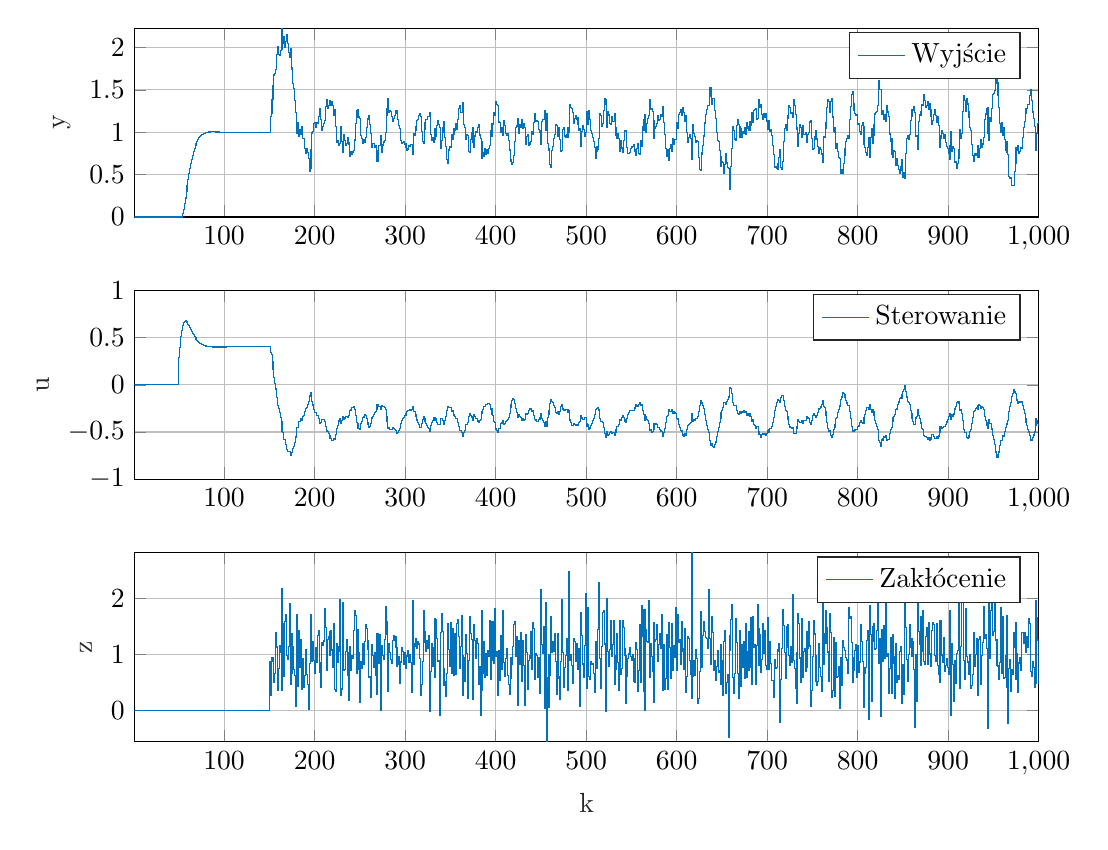
\begin{tikzpicture}

\begin{axis}[%
width=4.521in,
height=0.944in,
at={(0.758in,1.792in)},
scale only axis,
xmin=1,
xmax=1000,
ymin=-1,
ymax=1,
ylabel style={font=\color{white!15!black}},
ylabel={u},
axis background/.style={fill=white},
xmajorgrids,
ymajorgrids,
legend style={legend cell align=left, align=left, draw=white!15!black}
]
\addplot[const plot, color=mycolor1] table[row sep=crcr] {%
1	0\\
2	0\\
3	0\\
4	0\\
5	0\\
6	0\\
7	0\\
8	0\\
9	0\\
10	0\\
11	0\\
12	0\\
13	0\\
14	0\\
15	0\\
16	0\\
17	0\\
18	0\\
19	0\\
20	0\\
21	0\\
22	0\\
23	0\\
24	0\\
25	0\\
26	0\\
27	0\\
28	0\\
29	0\\
30	0\\
31	0\\
32	0\\
33	0\\
34	0\\
35	0\\
36	0\\
37	0\\
38	0\\
39	0\\
40	0\\
41	0\\
42	0\\
43	0\\
44	0\\
45	0\\
46	0\\
47	0\\
48	0\\
49	0\\
50	0.28956\\
51	0.39251\\
52	0.5131\\
53	0.58007\\
54	0.63135\\
55	0.65951\\
56	0.67407\\
57	0.67664\\
58	0.67103\\
59	0.65931\\
60	0.64358\\
61	0.62529\\
62	0.60567\\
63	0.58562\\
64	0.56581\\
65	0.54674\\
66	0.52873\\
67	0.512\\
68	0.49669\\
69	0.48283\\
70	0.47042\\
71	0.45942\\
72	0.44977\\
73	0.44136\\
74	0.4341\\
75	0.42788\\
76	0.4226\\
77	0.41815\\
78	0.41444\\
79	0.41136\\
80	0.40884\\
81	0.4068\\
82	0.40516\\
83	0.40387\\
84	0.40286\\
85	0.40209\\
86	0.40151\\
87	0.4011\\
88	0.40081\\
89	0.40063\\
90	0.40052\\
91	0.40048\\
92	0.40048\\
93	0.40051\\
94	0.40057\\
95	0.40065\\
96	0.40073\\
97	0.40082\\
98	0.40091\\
99	0.401\\
100	0.40108\\
101	0.40116\\
102	0.40123\\
103	0.4013\\
104	0.40136\\
105	0.40142\\
106	0.40146\\
107	0.4015\\
108	0.40154\\
109	0.40157\\
110	0.4016\\
111	0.40162\\
112	0.40164\\
113	0.40166\\
114	0.40167\\
115	0.40168\\
116	0.40169\\
117	0.4017\\
118	0.4017\\
119	0.40171\\
120	0.40171\\
121	0.40171\\
122	0.40171\\
123	0.40172\\
124	0.40172\\
125	0.40172\\
126	0.40172\\
127	0.40172\\
128	0.40172\\
129	0.40172\\
130	0.40172\\
131	0.40172\\
132	0.40172\\
133	0.40171\\
134	0.40171\\
135	0.40171\\
136	0.40171\\
137	0.40171\\
138	0.40171\\
139	0.40171\\
140	0.40171\\
141	0.40171\\
142	0.40171\\
143	0.40171\\
144	0.40171\\
145	0.40171\\
146	0.40171\\
147	0.40171\\
148	0.40171\\
149	0.40171\\
150	0.40171\\
151	0.34715\\
152	0.31696\\
153	0.24317\\
154	0.16286\\
155	0.075952\\
156	0.015852\\
157	-0.0442\\
158	-0.13848\\
159	-0.22071\\
160	-0.2555\\
161	-0.29439\\
162	-0.34432\\
163	-0.3874\\
164	-0.49819\\
165	-0.50802\\
166	-0.57908\\
167	-0.57734\\
168	-0.6306\\
169	-0.68327\\
170	-0.70197\\
171	-0.70492\\
172	-0.70633\\
173	-0.74971\\
174	-0.71247\\
175	-0.72092\\
176	-0.67544\\
177	-0.6572\\
178	-0.60748\\
179	-0.55246\\
180	-0.45538\\
181	-0.45102\\
182	-0.38381\\
183	-0.38831\\
184	-0.35633\\
185	-0.36477\\
186	-0.37252\\
187	-0.33902\\
188	-0.32823\\
189	-0.28181\\
190	-0.24712\\
191	-0.23617\\
192	-0.20937\\
193	-0.17498\\
194	-0.10836\\
195	-0.084426\\
196	-0.11997\\
197	-0.1807\\
198	-0.21393\\
199	-0.26492\\
200	-0.29021\\
201	-0.29748\\
202	-0.32052\\
203	-0.32543\\
204	-0.35867\\
205	-0.39816\\
206	-0.41047\\
207	-0.40381\\
208	-0.36779\\
209	-0.36929\\
210	-0.37019\\
211	-0.3865\\
212	-0.44162\\
213	-0.48868\\
214	-0.49368\\
215	-0.5176\\
216	-0.5371\\
217	-0.56478\\
218	-0.56635\\
219	-0.58939\\
220	-0.58823\\
221	-0.56588\\
222	-0.57982\\
223	-0.52597\\
224	-0.4622\\
225	-0.4329\\
226	-0.39213\\
227	-0.37695\\
228	-0.36197\\
229	-0.41177\\
230	-0.37353\\
231	-0.33567\\
232	-0.37074\\
233	-0.35191\\
234	-0.33921\\
235	-0.33334\\
236	-0.34543\\
237	-0.3243\\
238	-0.32443\\
239	-0.26979\\
240	-0.26711\\
241	-0.23903\\
242	-0.23589\\
243	-0.22942\\
244	-0.26018\\
245	-0.32217\\
246	-0.39465\\
247	-0.41121\\
248	-0.46125\\
249	-0.45841\\
250	-0.46829\\
251	-0.41173\\
252	-0.38677\\
253	-0.34706\\
254	-0.34121\\
255	-0.31854\\
256	-0.32672\\
257	-0.35757\\
258	-0.3983\\
259	-0.42282\\
260	-0.453\\
261	-0.43868\\
262	-0.41359\\
263	-0.35159\\
264	-0.33685\\
265	-0.31518\\
266	-0.29302\\
267	-0.28582\\
268	-0.25865\\
269	-0.21061\\
270	-0.22067\\
271	-0.22569\\
272	-0.22882\\
273	-0.26083\\
274	-0.21572\\
275	-0.23024\\
276	-0.23002\\
277	-0.23714\\
278	-0.26449\\
279	-0.3339\\
280	-0.38762\\
281	-0.45918\\
282	-0.45057\\
283	-0.4755\\
284	-0.47688\\
285	-0.47265\\
286	-0.45653\\
287	-0.46079\\
288	-0.47259\\
289	-0.48645\\
290	-0.50667\\
291	-0.51588\\
292	-0.50204\\
293	-0.48104\\
294	-0.46136\\
295	-0.41111\\
296	-0.37853\\
297	-0.36043\\
298	-0.34823\\
299	-0.32898\\
300	-0.32268\\
301	-0.30114\\
302	-0.28031\\
303	-0.27054\\
304	-0.27062\\
305	-0.26413\\
306	-0.26766\\
307	-0.26389\\
308	-0.2274\\
309	-0.28231\\
310	-0.28258\\
311	-0.31519\\
312	-0.33743\\
313	-0.37222\\
314	-0.39516\\
315	-0.42419\\
316	-0.44772\\
317	-0.45404\\
318	-0.41256\\
319	-0.36614\\
320	-0.33279\\
321	-0.36011\\
322	-0.38492\\
323	-0.41236\\
324	-0.42782\\
325	-0.45194\\
326	-0.4644\\
327	-0.48946\\
328	-0.42957\\
329	-0.39568\\
330	-0.37892\\
331	-0.3497\\
332	-0.3446\\
333	-0.37465\\
334	-0.35558\\
335	-0.39637\\
336	-0.41832\\
337	-0.42483\\
338	-0.42206\\
339	-0.35226\\
340	-0.355\\
341	-0.38174\\
342	-0.41457\\
343	-0.39365\\
344	-0.37852\\
345	-0.33641\\
346	-0.2739\\
347	-0.22683\\
348	-0.23704\\
349	-0.23992\\
350	-0.23735\\
351	-0.27943\\
352	-0.27546\\
353	-0.32003\\
354	-0.31181\\
355	-0.33186\\
356	-0.36072\\
357	-0.35368\\
358	-0.39484\\
359	-0.44227\\
360	-0.48389\\
361	-0.48748\\
362	-0.5018\\
363	-0.54242\\
364	-0.5473\\
365	-0.50417\\
366	-0.48061\\
367	-0.4238\\
368	-0.41822\\
369	-0.3976\\
370	-0.33891\\
371	-0.30901\\
372	-0.32735\\
373	-0.34912\\
374	-0.37762\\
375	-0.34131\\
376	-0.31965\\
377	-0.3376\\
378	-0.35372\\
379	-0.35938\\
380	-0.38336\\
381	-0.40256\\
382	-0.37923\\
383	-0.36272\\
384	-0.28404\\
385	-0.30834\\
386	-0.25756\\
387	-0.23358\\
388	-0.23366\\
389	-0.20963\\
390	-0.21279\\
391	-0.1932\\
392	-0.20244\\
393	-0.20753\\
394	-0.25876\\
395	-0.25507\\
396	-0.31127\\
397	-0.32501\\
398	-0.38485\\
399	-0.39718\\
400	-0.46772\\
401	-0.48533\\
402	-0.50757\\
403	-0.46585\\
404	-0.4584\\
405	-0.4112\\
406	-0.41305\\
407	-0.39966\\
408	-0.37736\\
409	-0.41471\\
410	-0.40809\\
411	-0.3891\\
412	-0.37573\\
413	-0.37169\\
414	-0.34263\\
415	-0.30035\\
416	-0.23883\\
417	-0.21171\\
418	-0.16869\\
419	-0.14895\\
420	-0.1524\\
421	-0.1933\\
422	-0.25396\\
423	-0.2886\\
424	-0.34066\\
425	-0.31174\\
426	-0.33632\\
427	-0.34627\\
428	-0.34688\\
429	-0.37638\\
430	-0.35614\\
431	-0.37502\\
432	-0.36298\\
433	-0.30877\\
434	-0.31482\\
435	-0.30782\\
436	-0.27237\\
437	-0.25927\\
438	-0.25175\\
439	-0.24844\\
440	-0.27852\\
441	-0.27659\\
442	-0.32593\\
443	-0.37198\\
444	-0.37296\\
445	-0.38753\\
446	-0.39066\\
447	-0.37004\\
448	-0.36193\\
449	-0.34801\\
450	-0.30051\\
451	-0.35811\\
452	-0.37434\\
453	-0.39666\\
454	-0.43736\\
455	-0.39243\\
456	-0.4462\\
457	-0.3498\\
458	-0.31109\\
459	-0.27579\\
460	-0.20186\\
461	-0.15627\\
462	-0.17632\\
463	-0.18405\\
464	-0.2169\\
465	-0.24143\\
466	-0.28872\\
467	-0.30802\\
468	-0.28776\\
469	-0.31561\\
470	-0.29833\\
471	-0.27921\\
472	-0.2253\\
473	-0.20537\\
474	-0.25579\\
475	-0.27559\\
476	-0.26618\\
477	-0.26173\\
478	-0.26436\\
479	-0.2893\\
480	-0.26438\\
481	-0.27742\\
482	-0.37215\\
483	-0.3985\\
484	-0.43228\\
485	-0.43523\\
486	-0.41127\\
487	-0.42134\\
488	-0.43005\\
489	-0.42524\\
490	-0.43499\\
491	-0.41766\\
492	-0.39581\\
493	-0.39007\\
494	-0.32392\\
495	-0.35105\\
496	-0.36316\\
497	-0.36408\\
498	-0.34294\\
499	-0.34809\\
500	-0.41216\\
501	-0.44031\\
502	-0.42495\\
503	-0.47659\\
504	-0.45751\\
505	-0.43312\\
506	-0.408\\
507	-0.37966\\
508	-0.35266\\
509	-0.31574\\
510	-0.25756\\
511	-0.24982\\
512	-0.2472\\
513	-0.23603\\
514	-0.26647\\
515	-0.35736\\
516	-0.38985\\
517	-0.38599\\
518	-0.40154\\
519	-0.44942\\
520	-0.51225\\
521	-0.54743\\
522	-0.55902\\
523	-0.49772\\
524	-0.53589\\
525	-0.52295\\
526	-0.50654\\
527	-0.49421\\
528	-0.51507\\
529	-0.5055\\
530	-0.50953\\
531	-0.536\\
532	-0.50074\\
533	-0.47079\\
534	-0.44248\\
535	-0.44239\\
536	-0.41886\\
537	-0.36702\\
538	-0.38031\\
539	-0.34478\\
540	-0.32196\\
541	-0.34291\\
542	-0.37226\\
543	-0.3919\\
544	-0.40222\\
545	-0.35375\\
546	-0.31692\\
547	-0.2895\\
548	-0.27471\\
549	-0.27485\\
550	-0.27311\\
551	-0.27107\\
552	-0.27501\\
553	-0.25065\\
554	-0.24582\\
555	-0.21389\\
556	-0.22485\\
557	-0.23259\\
558	-0.20508\\
559	-0.19128\\
560	-0.22337\\
561	-0.2078\\
562	-0.27567\\
563	-0.31745\\
564	-0.3117\\
565	-0.37537\\
566	-0.33177\\
567	-0.36695\\
568	-0.38098\\
569	-0.40864\\
570	-0.47865\\
571	-0.47588\\
572	-0.50024\\
573	-0.49767\\
574	-0.47716\\
575	-0.41051\\
576	-0.41677\\
577	-0.41124\\
578	-0.42452\\
579	-0.45622\\
580	-0.4558\\
581	-0.46943\\
582	-0.48959\\
583	-0.49833\\
584	-0.54167\\
585	-0.50624\\
586	-0.50895\\
587	-0.45861\\
588	-0.39871\\
589	-0.33691\\
590	-0.32341\\
591	-0.26513\\
592	-0.28313\\
593	-0.28329\\
594	-0.26613\\
595	-0.29969\\
596	-0.29009\\
597	-0.28821\\
598	-0.29852\\
599	-0.30171\\
600	-0.3604\\
601	-0.36194\\
602	-0.42296\\
603	-0.45181\\
604	-0.48843\\
605	-0.48898\\
606	-0.52797\\
607	-0.53597\\
608	-0.54236\\
609	-0.51892\\
610	-0.53237\\
611	-0.4767\\
612	-0.43107\\
613	-0.41682\\
614	-0.41318\\
615	-0.39684\\
616	-0.36578\\
617	-0.30236\\
618	-0.38906\\
619	-0.3709\\
620	-0.38095\\
621	-0.35336\\
622	-0.35314\\
623	-0.34023\\
624	-0.28242\\
625	-0.21677\\
626	-0.17042\\
627	-0.19581\\
628	-0.18569\\
629	-0.21714\\
630	-0.25308\\
631	-0.31605\\
632	-0.37333\\
633	-0.42677\\
634	-0.47271\\
635	-0.50208\\
636	-0.58781\\
637	-0.62664\\
638	-0.63866\\
639	-0.62528\\
640	-0.64994\\
641	-0.66048\\
642	-0.63479\\
643	-0.60614\\
644	-0.54578\\
645	-0.49393\\
646	-0.45657\\
647	-0.40325\\
648	-0.35402\\
649	-0.2897\\
650	-0.26996\\
651	-0.24307\\
652	-0.18939\\
653	-0.18846\\
654	-0.2082\\
655	-0.17923\\
656	-0.15536\\
657	-0.12926\\
658	-0.036648\\
659	-0.025241\\
660	-0.037226\\
661	-0.096165\\
662	-0.18915\\
663	-0.21976\\
664	-0.22176\\
665	-0.21955\\
666	-0.26926\\
667	-0.30366\\
668	-0.31249\\
669	-0.28092\\
670	-0.30644\\
671	-0.30222\\
672	-0.27836\\
673	-0.28815\\
674	-0.27689\\
675	-0.29685\\
676	-0.27887\\
677	-0.31979\\
678	-0.30596\\
679	-0.32148\\
680	-0.30877\\
681	-0.33974\\
682	-0.3348\\
683	-0.38607\\
684	-0.3677\\
685	-0.41911\\
686	-0.4356\\
687	-0.46291\\
688	-0.43821\\
689	-0.44435\\
690	-0.49026\\
691	-0.52784\\
692	-0.53028\\
693	-0.55386\\
694	-0.53031\\
695	-0.51408\\
696	-0.52731\\
697	-0.51781\\
698	-0.53537\\
699	-0.51461\\
700	-0.48642\\
701	-0.50423\\
702	-0.47598\\
703	-0.4639\\
704	-0.45952\\
705	-0.43771\\
706	-0.39529\\
707	-0.34469\\
708	-0.26966\\
709	-0.23099\\
710	-0.18999\\
711	-0.16184\\
712	-0.15652\\
713	-0.1643\\
714	-0.18871\\
715	-0.1334\\
716	-0.10897\\
717	-0.10837\\
718	-0.16629\\
719	-0.22827\\
720	-0.27428\\
721	-0.28488\\
722	-0.3376\\
723	-0.36686\\
724	-0.42486\\
725	-0.44704\\
726	-0.45345\\
727	-0.46554\\
728	-0.45675\\
729	-0.51889\\
730	-0.52016\\
731	-0.51317\\
732	-0.46554\\
733	-0.44564\\
734	-0.36781\\
735	-0.38387\\
736	-0.39978\\
737	-0.4026\\
738	-0.37423\\
739	-0.40456\\
740	-0.37738\\
741	-0.37945\\
742	-0.37716\\
743	-0.35694\\
744	-0.33556\\
745	-0.35015\\
746	-0.35585\\
747	-0.3981\\
748	-0.41941\\
749	-0.37682\\
750	-0.32905\\
751	-0.30188\\
752	-0.32065\\
753	-0.34353\\
754	-0.32625\\
755	-0.32818\\
756	-0.29224\\
757	-0.25616\\
758	-0.25335\\
759	-0.23485\\
760	-0.21181\\
761	-0.16765\\
762	-0.23318\\
763	-0.2375\\
764	-0.28794\\
765	-0.32231\\
766	-0.39797\\
767	-0.45886\\
768	-0.49626\\
769	-0.48767\\
770	-0.53399\\
771	-0.56067\\
772	-0.52257\\
773	-0.46962\\
774	-0.45514\\
775	-0.42233\\
776	-0.35863\\
777	-0.34336\\
778	-0.2961\\
779	-0.25691\\
780	-0.22395\\
781	-0.15155\\
782	-0.1291\\
783	-0.08236\\
784	-0.093779\\
785	-0.10789\\
786	-0.13517\\
787	-0.16657\\
788	-0.19259\\
789	-0.21455\\
790	-0.21834\\
791	-0.28701\\
792	-0.35469\\
793	-0.43844\\
794	-0.49311\\
795	-0.49664\\
796	-0.48915\\
797	-0.47866\\
798	-0.47264\\
799	-0.47288\\
800	-0.4406\\
801	-0.43621\\
802	-0.40233\\
803	-0.38058\\
804	-0.39638\\
805	-0.40754\\
806	-0.40464\\
807	-0.34621\\
808	-0.31437\\
809	-0.27022\\
810	-0.23923\\
811	-0.23989\\
812	-0.2647\\
813	-0.20669\\
814	-0.25905\\
815	-0.28739\\
816	-0.26362\\
817	-0.2855\\
818	-0.32146\\
819	-0.37607\\
820	-0.40807\\
821	-0.43717\\
822	-0.47735\\
823	-0.58678\\
824	-0.60876\\
825	-0.6494\\
826	-0.58325\\
827	-0.58933\\
828	-0.57354\\
829	-0.54947\\
830	-0.55784\\
831	-0.5363\\
832	-0.58764\\
833	-0.58045\\
834	-0.57939\\
835	-0.51958\\
836	-0.47427\\
837	-0.45403\\
838	-0.38482\\
839	-0.34437\\
840	-0.33407\\
841	-0.31732\\
842	-0.26207\\
843	-0.25637\\
844	-0.21277\\
845	-0.18199\\
846	-0.14259\\
847	-0.13729\\
848	-0.14609\\
849	-0.10597\\
850	-0.067\\
851	-0.050876\\
852	-0.010046\\
853	-0.073251\\
854	-0.12878\\
855	-0.17271\\
856	-0.18469\\
857	-0.2131\\
858	-0.2688\\
859	-0.30855\\
860	-0.35914\\
861	-0.38532\\
862	-0.4224\\
863	-0.42315\\
864	-0.35133\\
865	-0.33178\\
866	-0.25772\\
867	-0.32747\\
868	-0.35702\\
869	-0.39826\\
870	-0.4058\\
871	-0.45967\\
872	-0.47648\\
873	-0.53914\\
874	-0.54573\\
875	-0.54369\\
876	-0.55476\\
877	-0.57596\\
878	-0.56245\\
879	-0.58794\\
880	-0.57873\\
881	-0.56216\\
882	-0.52854\\
883	-0.52968\\
884	-0.54508\\
885	-0.57108\\
886	-0.56788\\
887	-0.55228\\
888	-0.56734\\
889	-0.54178\\
890	-0.5033\\
891	-0.44319\\
892	-0.4444\\
893	-0.4583\\
894	-0.45425\\
895	-0.43982\\
896	-0.44568\\
897	-0.41757\\
898	-0.39343\\
899	-0.36996\\
900	-0.33934\\
901	-0.30076\\
902	-0.32393\\
903	-0.36881\\
904	-0.31992\\
905	-0.3305\\
906	-0.30935\\
907	-0.25598\\
908	-0.23183\\
909	-0.18411\\
910	-0.17406\\
911	-0.17295\\
912	-0.19546\\
913	-0.26916\\
914	-0.26526\\
915	-0.29921\\
916	-0.38\\
917	-0.47123\\
918	-0.50853\\
919	-0.50943\\
920	-0.56218\\
921	-0.56493\\
922	-0.55995\\
923	-0.5394\\
924	-0.49902\\
925	-0.47246\\
926	-0.40835\\
927	-0.34405\\
928	-0.28487\\
929	-0.27629\\
930	-0.24792\\
931	-0.24264\\
932	-0.25676\\
933	-0.21982\\
934	-0.20759\\
935	-0.2194\\
936	-0.24777\\
937	-0.23305\\
938	-0.24338\\
939	-0.26301\\
940	-0.33147\\
941	-0.37781\\
942	-0.43208\\
943	-0.46408\\
944	-0.40163\\
945	-0.36615\\
946	-0.41317\\
947	-0.41007\\
948	-0.468\\
949	-0.53517\\
950	-0.58257\\
951	-0.62807\\
952	-0.71114\\
953	-0.74329\\
954	-0.7691\\
955	-0.7487\\
956	-0.71213\\
957	-0.64563\\
958	-0.58768\\
959	-0.58788\\
960	-0.53528\\
961	-0.54763\\
962	-0.49662\\
963	-0.44868\\
964	-0.41038\\
965	-0.4228\\
966	-0.37336\\
967	-0.2822\\
968	-0.22777\\
969	-0.18517\\
970	-0.12476\\
971	-0.090367\\
972	-0.055016\\
973	-0.075458\\
974	-0.09493\\
975	-0.15635\\
976	-0.16454\\
977	-0.19687\\
978	-0.17682\\
979	-0.1817\\
980	-0.18593\\
981	-0.18182\\
982	-0.21749\\
983	-0.26108\\
984	-0.30339\\
985	-0.35717\\
986	-0.40105\\
987	-0.43093\\
988	-0.46873\\
989	-0.49095\\
990	-0.54114\\
991	-0.58716\\
992	-0.58415\\
993	-0.55921\\
994	-0.53161\\
995	-0.4919\\
996	-0.42839\\
997	-0.36141\\
998	-0.38272\\
999	-0.40969\\
1000	-0.43619\\
};
\addlegendentry{Sterowanie}

\end{axis}

\begin{axis}[%
width=4.521in,
height=0.944in,
at={(0.758in,3.103in)},
scale only axis,
xmin=1,
xmax=1000,
ymin=0,
ymax=2.2273,
ylabel style={font=\color{white!15!black}},
ylabel={y},
axis background/.style={fill=white},
xmajorgrids,
ymajorgrids,
legend style={legend cell align=left, align=left, draw=white!15!black}
]
\addplot[const plot, color=mycolor1] table[row sep=crcr] {%
1	0\\
2	0\\
3	0\\
4	0\\
5	0\\
6	0\\
7	0\\
8	0\\
9	0\\
10	0\\
11	0\\
12	0\\
13	0\\
14	0\\
15	0\\
16	0\\
17	0\\
18	0\\
19	0\\
20	0\\
21	0\\
22	0\\
23	0\\
24	0\\
25	0\\
26	0\\
27	0\\
28	0\\
29	0\\
30	0\\
31	0\\
32	0\\
33	0\\
34	0\\
35	0\\
36	0\\
37	0\\
38	0\\
39	0\\
40	0\\
41	0\\
42	0\\
43	0\\
44	0\\
45	0\\
46	0\\
47	0\\
48	0\\
49	0\\
50	0\\
51	0\\
52	0\\
53	0\\
54	0.039119\\
55	0.090032\\
56	0.15448\\
57	0.22449\\
58	0.29764\\
59	0.37063\\
60	0.44164\\
61	0.50914\\
62	0.57223\\
63	0.63032\\
64	0.68313\\
65	0.73061\\
66	0.77286\\
67	0.81011\\
68	0.84266\\
69	0.87086\\
70	0.8951\\
71	0.91576\\
72	0.93322\\
73	0.94786\\
74	0.96003\\
75	0.97004\\
76	0.97821\\
77	0.98479\\
78	0.99003\\
79	0.99414\\
80	0.99731\\
81	0.99971\\
82	1.0015\\
83	1.0027\\
84	1.0036\\
85	1.0041\\
86	1.0043\\
87	1.0044\\
88	1.0043\\
89	1.0042\\
90	1.0039\\
91	1.0036\\
92	1.0033\\
93	1.003\\
94	1.0027\\
95	1.0024\\
96	1.0021\\
97	1.0018\\
98	1.0016\\
99	1.0013\\
100	1.0011\\
101	1.001\\
102	1.0008\\
103	1.0007\\
104	1.0005\\
105	1.0004\\
106	1.0003\\
107	1.0003\\
108	1.0002\\
109	1.0002\\
110	1.0001\\
111	1.0001\\
112	1.0001\\
113	1\\
114	1\\
115	1\\
116	1\\
117	0.99999\\
118	0.99998\\
119	0.99998\\
120	0.99998\\
121	0.99998\\
122	0.99998\\
123	0.99998\\
124	0.99998\\
125	0.99998\\
126	0.99998\\
127	0.99998\\
128	0.99998\\
129	0.99998\\
130	0.99998\\
131	0.99998\\
132	0.99999\\
133	0.99999\\
134	0.99999\\
135	0.99999\\
136	0.99999\\
137	0.99999\\
138	0.99999\\
139	0.99999\\
140	0.99999\\
141	0.99999\\
142	0.99999\\
143	0.99999\\
144	0.99999\\
145	0.99999\\
146	0.99999\\
147	0.99999\\
148	0.99999\\
149	0.99999\\
150	0.99999\\
151	1.1884\\
152	1.2257\\
153	1.3888\\
154	1.549\\
155	1.6749\\
156	1.6947\\
157	1.7361\\
158	1.9181\\
159	2.0094\\
160	1.9144\\
161	1.9032\\
162	1.9666\\
163	1.9815\\
164	2.2273\\
165	2.0482\\
166	2.1347\\
167	1.9995\\
168	2.0698\\
169	2.1493\\
170	2.0496\\
171	1.9441\\
172	1.8854\\
173	1.9856\\
174	1.7575\\
175	1.7463\\
176	1.5786\\
177	1.519\\
178	1.3792\\
179	1.2303\\
180	0.98104\\
181	1.1097\\
182	0.9542\\
183	1.0328\\
184	0.97447\\
185	1.0251\\
186	1.0705\\
187	0.9311\\
188	0.9267\\
189	0.81209\\
190	0.75571\\
191	0.80665\\
192	0.76024\\
193	0.68726\\
194	0.53205\\
195	0.57075\\
196	0.79568\\
197	0.9916\\
198	1.009\\
199	1.1013\\
200	1.1091\\
201	1.0615\\
202	1.1148\\
203	1.0986\\
204	1.1836\\
205	1.2742\\
206	1.2322\\
207	1.1535\\
208	1.0222\\
209	1.0712\\
210	1.0997\\
211	1.1435\\
212	1.3085\\
213	1.3827\\
214	1.2839\\
215	1.3119\\
216	1.3394\\
217	1.3759\\
218	1.3182\\
219	1.3571\\
220	1.3121\\
221	1.1991\\
222	1.2639\\
223	1.0686\\
224	0.88539\\
225	0.90607\\
226	0.84975\\
227	0.8651\\
228	0.86839\\
229	1.071\\
230	0.89435\\
231	0.76321\\
232	0.97697\\
233	0.90485\\
234	0.84973\\
235	0.87214\\
236	0.93559\\
237	0.85696\\
238	0.87571\\
239	0.71383\\
240	0.77399\\
241	0.74022\\
242	0.76765\\
243	0.78557\\
244	0.9091\\
245	1.1014\\
246	1.2537\\
247	1.1713\\
248	1.2621\\
249	1.1812\\
250	1.1667\\
251	0.96127\\
252	0.92696\\
253	0.87093\\
254	0.91343\\
255	0.8775\\
256	0.93577\\
257	1.0565\\
258	1.1517\\
259	1.1597\\
260	1.198\\
261	1.0904\\
262	0.99042\\
263	0.81964\\
264	0.86318\\
265	0.86235\\
266	0.82045\\
267	0.84547\\
268	0.7841\\
269	0.66152\\
270	0.78756\\
271	0.8446\\
272	0.84327\\
273	0.95599\\
274	0.7672\\
275	0.84912\\
276	0.8855\\
277	0.89766\\
278	0.99243\\
279	1.1978\\
280	1.2772\\
281	1.396\\
282	1.2324\\
283	1.2591\\
284	1.2411\\
285	1.1889\\
286	1.1295\\
287	1.1579\\
288	1.1993\\
289	1.2182\\
290	1.2519\\
291	1.2384\\
292	1.1522\\
293	1.0804\\
294	1.0434\\
295	0.90457\\
296	0.86402\\
297	0.8844\\
298	0.88924\\
299	0.85299\\
300	0.86753\\
301	0.82219\\
302	0.78523\\
303	0.80293\\
304	0.8395\\
305	0.8315\\
306	0.85816\\
307	0.8549\\
308	0.73668\\
309	0.98235\\
310	0.95873\\
311	1.02\\
312	1.069\\
313	1.1336\\
314	1.1542\\
315	1.1945\\
316	1.2196\\
317	1.1825\\
318	1.006\\
319	0.88613\\
320	0.86287\\
321	1.0346\\
322	1.1131\\
323	1.1473\\
324	1.146\\
325	1.1845\\
326	1.1825\\
327	1.227\\
328	0.97406\\
329	0.90039\\
330	0.93929\\
331	0.88087\\
332	0.91029\\
333	1.0477\\
334	0.94852\\
335	1.0849\\
336	1.1345\\
337	1.0883\\
338	1.0533\\
339	0.80951\\
340	0.90524\\
341	1.061\\
342	1.1314\\
343	0.99468\\
344	0.93916\\
345	0.83563\\
346	0.68299\\
347	0.63772\\
348	0.79102\\
349	0.83465\\
350	0.8164\\
351	0.97319\\
352	0.91978\\
353	1.0448\\
354	0.97679\\
355	1.016\\
356	1.1072\\
357	1.0283\\
358	1.1535\\
359	1.2763\\
360	1.3185\\
361	1.2341\\
362	1.2369\\
363	1.3519\\
364	1.2953\\
365	1.0914\\
366	1.0511\\
367	0.91536\\
368	0.97471\\
369	0.95754\\
370	0.77584\\
371	0.76323\\
372	0.9194\\
373	0.99826\\
374	1.0539\\
375	0.87925\\
376	0.82659\\
377	0.95636\\
378	1.0099\\
379	0.99338\\
380	1.0589\\
381	1.0942\\
382	0.96823\\
383	0.92352\\
384	0.69628\\
385	0.88995\\
386	0.76231\\
387	0.71321\\
388	0.80201\\
389	0.74393\\
390	0.79041\\
391	0.75204\\
392	0.81175\\
393	0.84757\\
394	1.0167\\
395	0.94652\\
396	1.1029\\
397	1.0965\\
398	1.2336\\
399	1.1967\\
400	1.366\\
401	1.3308\\
402	1.3109\\
403	1.1208\\
404	1.1148\\
405	0.99308\\
406	1.0499\\
407	1.0396\\
408	0.96636\\
409	1.1324\\
410	1.0813\\
411	0.9823\\
412	0.96773\\
413	0.98527\\
414	0.89913\\
415	0.79058\\
416	0.65852\\
417	0.6807\\
418	0.62612\\
419	0.63857\\
420	0.72486\\
421	0.889\\
422	1.0562\\
423	1.0741\\
424	1.1659\\
425	0.98055\\
426	1.0554\\
427	1.0938\\
428	1.0549\\
429	1.1477\\
430	1.0399\\
431	1.0981\\
432	1.0534\\
433	0.85645\\
434	0.95471\\
435	0.97281\\
436	0.84648\\
437	0.85345\\
438	0.87935\\
439	0.88904\\
440	1.0072\\
441	0.97075\\
442	1.1178\\
443	1.2249\\
444	1.1244\\
445	1.1331\\
446	1.1269\\
447	1.0328\\
448	1.0237\\
449	1.0014\\
450	0.85612\\
451	1.1234\\
452	1.1528\\
453	1.1476\\
454	1.2504\\
455	1.0218\\
456	1.2202\\
457	0.8645\\
458	0.78501\\
459	0.80723\\
460	0.62018\\
461	0.58615\\
462	0.78561\\
463	0.83324\\
464	0.92383\\
465	0.9744\\
466	1.0857\\
467	1.0813\\
468	0.94849\\
469	1.0579\\
470	0.98662\\
471	0.91202\\
472	0.7695\\
473	0.78382\\
474	1.0353\\
475	1.0596\\
476	0.95615\\
477	0.94229\\
478	0.97011\\
479	1.0578\\
480	0.93974\\
481	0.99237\\
482	1.3317\\
483	1.2913\\
484	1.283\\
485	1.2323\\
486	1.1077\\
487	1.1635\\
488	1.1958\\
489	1.1474\\
490	1.1718\\
491	1.0979\\
492	1.0259\\
493	1.044\\
494	0.836\\
495	1.0095\\
496	1.0801\\
497	1.0335\\
498	0.95068\\
499	0.99396\\
500	1.2289\\
501	1.2397\\
502	1.0886\\
503	1.2619\\
504	1.1454\\
505	1.0256\\
506	0.98665\\
507	0.93453\\
508	0.89317\\
509	0.82111\\
510	0.68826\\
511	0.76785\\
512	0.82571\\
513	0.79823\\
514	0.92718\\
515	1.2228\\
516	1.2\\
517	1.0661\\
518	1.1039\\
519	1.2552\\
520	1.3943\\
521	1.389\\
522	1.3224\\
523	1.0587\\
524	1.2457\\
525	1.2035\\
526	1.1074\\
527	1.0926\\
528	1.1851\\
529	1.129\\
530	1.1258\\
531	1.2175\\
532	1.0515\\
533	0.95915\\
534	0.9294\\
535	0.98402\\
536	0.92456\\
537	0.77036\\
538	0.90336\\
539	0.81455\\
540	0.76404\\
541	0.90601\\
542	1.006\\
543	1.0214\\
544	1.0124\\
545	0.82025\\
546	0.7468\\
547	0.74826\\
548	0.76528\\
549	0.81305\\
550	0.82635\\
551	0.82843\\
552	0.855\\
553	0.77621\\
554	0.79327\\
555	0.72121\\
556	0.8084\\
557	0.8616\\
558	0.75205\\
559	0.74116\\
560	0.90566\\
561	0.83205\\
562	1.0616\\
563	1.15\\
564	1.0167\\
565	1.214\\
566	0.99632\\
567	1.1065\\
568	1.1596\\
569	1.195\\
570	1.3899\\
571	1.2638\\
572	1.2786\\
573	1.2412\\
574	1.1381\\
575	0.92733\\
576	1.04\\
577	1.0681\\
578	1.1016\\
579	1.1974\\
580	1.1398\\
581	1.1536\\
582	1.2054\\
583	1.1914\\
584	1.3056\\
585	1.1166\\
586	1.1196\\
587	0.97343\\
588	0.81322\\
589	0.71698\\
590	0.79595\\
591	0.66614\\
592	0.8106\\
593	0.85217\\
594	0.77701\\
595	0.92516\\
596	0.87626\\
597	0.85455\\
598	0.91303\\
599	0.91838\\
600	1.1128\\
601	1.0495\\
602	1.2047\\
603	1.2363\\
604	1.2664\\
605	1.1986\\
606	1.2936\\
607	1.2692\\
608	1.234\\
609	1.132\\
610	1.1912\\
611	0.99602\\
612	0.88157\\
613	0.93713\\
614	0.97548\\
615	0.93054\\
616	0.84529\\
617	0.6809\\
618	1.0887\\
619	0.98266\\
620	0.95226\\
621	0.8768\\
622	0.90011\\
623	0.88683\\
624	0.70323\\
625	0.56409\\
626	0.54517\\
627	0.75579\\
628	0.73958\\
629	0.84421\\
630	0.95641\\
631	1.1098\\
632	1.2087\\
633	1.2717\\
634	1.3181\\
635	1.3152\\
636	1.5303\\
637	1.5268\\
638	1.4278\\
639	1.3233\\
640	1.3995\\
641	1.402\\
642	1.257\\
643	1.1649\\
644	1.0014\\
645	0.90681\\
646	0.88609\\
647	0.78449\\
648	0.70753\\
649	0.59443\\
650	0.65133\\
651	0.64788\\
652	0.51824\\
653	0.61802\\
654	0.75152\\
655	0.63795\\
656	0.58778\\
657	0.57301\\
658	0.32059\\
659	0.43418\\
660	0.59619\\
661	0.8067\\
662	1.0649\\
663	1.02\\
664	0.92006\\
665	0.90028\\
666	1.0821\\
667	1.1469\\
668	1.0896\\
669	0.94297\\
670	1.0639\\
671	1.0484\\
672	0.94098\\
673	1.01\\
674	0.98088\\
675	1.0507\\
676	0.97634\\
677	1.1186\\
678	1.0403\\
679	1.0677\\
680	1.0217\\
681	1.1251\\
682	1.0824\\
683	1.2311\\
684	1.1103\\
685	1.2552\\
686	1.2679\\
687	1.2828\\
688	1.1461\\
689	1.1633\\
690	1.3321\\
691	1.3873\\
692	1.296\\
693	1.3319\\
694	1.211\\
695	1.1476\\
696	1.2261\\
697	1.1783\\
698	1.2253\\
699	1.1333\\
700	1.0335\\
701	1.1432\\
702	1.0414\\
703	1.0073\\
704	1.0316\\
705	0.96595\\
706	0.84621\\
707	0.74254\\
708	0.58446\\
709	0.59037\\
710	0.57045\\
711	0.5631\\
712	0.62862\\
713	0.70039\\
714	0.79371\\
715	0.58091\\
716	0.55634\\
717	0.65578\\
718	0.88917\\
719	1.0462\\
720	1.087\\
721	1.0242\\
722	1.1618\\
723	1.1961\\
724	1.3104\\
725	1.2911\\
726	1.2273\\
727	1.2383\\
728	1.1799\\
729	1.3841\\
730	1.3124\\
731	1.2141\\
732	1.0525\\
733	1.0368\\
734	0.82777\\
735	0.98468\\
736	1.0896\\
737	1.0532\\
738	0.93757\\
739	1.0749\\
740	0.97079\\
741	0.97721\\
742	0.99641\\
743	0.92367\\
744	0.87731\\
745	0.97409\\
746	0.99608\\
747	1.1206\\
748	1.1406\\
749	0.92724\\
750	0.79744\\
751	0.80472\\
752	0.94475\\
753	1.0247\\
754	0.91967\\
755	0.93104\\
756	0.82694\\
757	0.74511\\
758	0.81868\\
759	0.79448\\
760	0.74291\\
761	0.64426\\
762	0.95359\\
763	0.93862\\
764	1.048\\
765	1.1166\\
766	1.292\\
767	1.3843\\
768	1.3672\\
769	1.2353\\
770	1.3667\\
771	1.4034\\
772	1.1803\\
773	1.01\\
774	1.0518\\
775	0.99222\\
776	0.81238\\
777	0.86306\\
778	0.77483\\
779	0.70569\\
780	0.68819\\
781	0.51748\\
782	0.56518\\
783	0.51002\\
784	0.63465\\
785	0.72945\\
786	0.80725\\
787	0.88686\\
788	0.92808\\
789	0.95677\\
790	0.93068\\
791	1.1518\\
792	1.3055\\
793	1.4478\\
794	1.4748\\
795	1.3398\\
796	1.255\\
797	1.217\\
798	1.2025\\
799	1.2068\\
800	1.0877\\
801	1.1004\\
802	1.011\\
803	0.97007\\
804	1.0781\\
805	1.1105\\
806	1.0661\\
807	0.85602\\
808	0.81869\\
809	0.76026\\
810	0.73235\\
811	0.81595\\
812	0.93225\\
813	0.705\\
814	0.9404\\
815	1.0415\\
816	0.87366\\
817	0.96294\\
818	1.0911\\
819	1.2149\\
820	1.2282\\
821	1.2398\\
822	1.3145\\
823	1.6122\\
824	1.5096\\
825	1.5085\\
826	1.2056\\
827	1.2514\\
828	1.2408\\
829	1.1467\\
830	1.2074\\
831	1.1322\\
832	1.3141\\
833	1.2388\\
834	1.1816\\
835	0.97955\\
836	0.88637\\
837	0.92229\\
838	0.74036\\
839	0.69847\\
840	0.77954\\
841	0.77066\\
842	0.61327\\
843	0.68542\\
844	0.60421\\
845	0.56228\\
846	0.51964\\
847	0.58956\\
848	0.67829\\
849	0.54736\\
850	0.47059\\
851	0.5207\\
852	0.45138\\
853	0.75085\\
854	0.92415\\
855	0.961\\
856	0.91841\\
857	0.97729\\
858	1.1367\\
859	1.1853\\
860	1.2634\\
861	1.2594\\
862	1.3069\\
863	1.2381\\
864	0.94728\\
865	0.96174\\
866	0.79178\\
867	1.1286\\
868	1.2136\\
869	1.2423\\
870	1.1957\\
871	1.3309\\
872	1.3139\\
873	1.4494\\
874	1.375\\
875	1.2879\\
876	1.3153\\
877	1.3626\\
878	1.2641\\
879	1.3347\\
880	1.273\\
881	1.1863\\
882	1.0889\\
883	1.1363\\
884	1.2083\\
885	1.2652\\
886	1.1993\\
887	1.1171\\
888	1.1853\\
889	1.0846\\
890	0.95833\\
891	0.81756\\
892	0.9246\\
893	1.0232\\
894	0.98427\\
895	0.92738\\
896	0.97201\\
897	0.8825\\
898	0.82763\\
899	0.8066\\
900	0.75321\\
901	0.68263\\
902	0.84378\\
903	1.013\\
904	0.77111\\
905	0.83451\\
906	0.80858\\
907	0.64073\\
908	0.65241\\
909	0.57573\\
910	0.62778\\
911	0.69335\\
912	0.79127\\
913	1.0333\\
914	0.92138\\
915	0.98508\\
916	1.243\\
917	1.4303\\
918	1.3744\\
919	1.2489\\
920	1.3961\\
921	1.3335\\
922	1.2491\\
923	1.1745\\
924	1.0517\\
925	1.0167\\
926	0.8548\\
927	0.72525\\
928	0.65556\\
929	0.75418\\
930	0.72191\\
931	0.74779\\
932	0.83956\\
933	0.7068\\
934	0.70575\\
935	0.80967\\
936	0.91144\\
937	0.82382\\
938	0.86099\\
939	0.94238\\
940	1.1504\\
941	1.2151\\
942	1.285\\
943	1.2921\\
944	0.98572\\
945	0.90811\\
946	1.1717\\
947	1.1256\\
948	1.2759\\
949	1.4417\\
950	1.4601\\
951	1.4917\\
952	1.6718\\
953	1.6263\\
954	1.581\\
955	1.4351\\
956	1.2881\\
957	1.1023\\
958	0.99526\\
959	1.1102\\
960	0.96435\\
961	1.0557\\
962	0.90996\\
963	0.78433\\
964	0.76023\\
965	0.89131\\
966	0.74075\\
967	0.47531\\
968	0.45585\\
969	0.4685\\
970	0.36863\\
971	0.37711\\
972	0.37204\\
973	0.53559\\
974	0.63324\\
975	0.82217\\
976	0.78182\\
977	0.84529\\
978	0.75192\\
979	0.77573\\
980	0.81947\\
981	0.80366\\
982	0.93875\\
983	1.0597\\
984	1.1253\\
985	1.2266\\
986	1.2785\\
987	1.2793\\
988	1.3323\\
989	1.3313\\
990	1.4343\\
991	1.503\\
992	1.3762\\
993	1.2391\\
994	1.1656\\
995	1.0698\\
996	0.90895\\
997	0.77991\\
998	0.98574\\
999	1.1079\\
1000	1.1376\\
};
\addlegendentry{Wyjście}

\end{axis}

\begin{axis}[%
width=4.521in,
height=0.944in,
at={(0.758in,0.481in)},
scale only axis,
xmin=1,
xmax=1000,
xlabel style={font=\color{white!15!black}},
xlabel={k},
ymin=-0.54717,
ymax=2.8218,
ylabel style={font=\color{white!15!black}},
ylabel={z},
axis background/.style={fill=white},
xmajorgrids,
ymajorgrids,
legend style={legend cell align=left, align=left, draw=white!15!black}
]
\addplot[const plot, color=mycolor1] table[row sep=crcr] {%
1	0\\
2	0\\
3	0\\
4	0\\
5	0\\
6	0\\
7	0\\
8	0\\
9	0\\
10	0\\
11	0\\
12	0\\
13	0\\
14	0\\
15	0\\
16	0\\
17	0\\
18	0\\
19	0\\
20	0\\
21	0\\
22	0\\
23	0\\
24	0\\
25	0\\
26	0\\
27	0\\
28	0\\
29	0\\
30	0\\
31	0\\
32	0\\
33	0\\
34	0\\
35	0\\
36	0\\
37	0\\
38	0\\
39	0\\
40	0\\
41	0\\
42	0\\
43	0\\
44	0\\
45	0\\
46	0\\
47	0\\
48	0\\
49	0\\
50	0\\
51	0\\
52	0\\
53	0\\
54	0\\
55	0\\
56	0\\
57	0\\
58	0\\
59	0\\
60	0\\
61	0\\
62	0\\
63	0\\
64	0\\
65	0\\
66	0\\
67	0\\
68	0\\
69	0\\
70	0\\
71	0\\
72	0\\
73	0\\
74	0\\
75	0\\
76	0\\
77	0\\
78	0\\
79	0\\
80	0\\
81	0\\
82	0\\
83	0\\
84	0\\
85	0\\
86	0\\
87	0\\
88	0\\
89	0\\
90	0\\
91	0\\
92	0\\
93	0\\
94	0\\
95	0\\
96	0\\
97	0\\
98	0\\
99	0\\
100	0\\
101	0\\
102	0\\
103	0\\
104	0\\
105	0\\
106	0\\
107	0\\
108	0\\
109	0\\
110	0\\
111	0\\
112	0\\
113	0\\
114	0\\
115	0\\
116	0\\
117	0\\
118	0\\
119	0\\
120	0\\
121	0\\
122	0\\
123	0\\
124	0\\
125	0\\
126	0\\
127	0\\
128	0\\
129	0\\
130	0\\
131	0\\
132	0\\
133	0\\
134	0\\
135	0\\
136	0\\
137	0\\
138	0\\
139	0\\
140	0\\
141	0\\
142	0\\
143	0\\
144	0\\
145	0\\
146	0\\
147	0\\
148	0\\
149	0\\
150	0.88354\\
151	0.27407\\
152	0.88366\\
153	0.95605\\
154	0.91393\\
155	0.50364\\
156	0.66573\\
157	1.403\\
158	1.1369\\
159	0.36008\\
160	0.75408\\
161	1.1722\\
162	1.0467\\
163	2.1786\\
164	0.35938\\
165	1.562\\
166	0.61562\\
167	1.599\\
168	1.7097\\
169	0.97881\\
170	0.92269\\
171	1.1428\\
172	1.9144\\
173	0.46379\\
174	1.3863\\
175	0.67005\\
176	1.1375\\
177	0.72851\\
178	0.63621\\
179	0.077369\\
180	1.7225\\
181	0.44033\\
182	1.4331\\
183	0.77979\\
184	1.2624\\
185	1.2259\\
186	0.38822\\
187	0.92944\\
188	0.41623\\
189	0.63472\\
190	1.0881\\
191	0.65137\\
192	0.4723\\
193	0.024057\\
194	0.84123\\
195	1.7143\\
196	1.6703\\
197	0.88887\\
198	1.2262\\
199	0.89267\\
200	0.66952\\
201	1.1349\\
202	0.86688\\
203	1.3489\\
204	1.4251\\
205	0.86604\\
206	0.67701\\
207	0.4117\\
208	1.2159\\
209	1.1577\\
210	1.2445\\
211	1.8171\\
212	1.4814\\
213	0.71207\\
214	1.2674\\
215	1.3173\\
216	1.4085\\
217	0.99516\\
218	1.4389\\
219	1.0849\\
220	0.7668\\
221	1.5492\\
222	0.38571\\
223	0.34646\\
224	1.1991\\
225	0.86368\\
226	1.1422\\
227	1.057\\
228	1.9759\\
229	0.27873\\
230	0.38802\\
231	1.925\\
232	0.72605\\
233	0.74321\\
234	1.0521\\
235	1.2754\\
236	0.62902\\
237	1.034\\
238	0.1906\\
239	1.1516\\
240	0.72736\\
241	0.9939\\
242	0.92655\\
243	1.4251\\
244	1.7905\\
245	1.6972\\
246	0.66743\\
247	1.4511\\
248	0.72954\\
249	1.0429\\
250	0.15256\\
251	0.88063\\
252	0.76286\\
253	1.2053\\
254	0.82777\\
255	1.2363\\
256	1.5351\\
257	1.4745\\
258	1.0998\\
259	1.2498\\
260	0.60322\\
261	0.6084\\
262	0.24034\\
263	1.1766\\
264	0.98544\\
265	0.77889\\
266	1.0327\\
267	0.6303\\
268	0.29568\\
269	1.3807\\
270	1.116\\
271	0.852\\
272	1.3518\\
273	-0.0018638\\
274	1.1666\\
275	0.99385\\
276	0.91568\\
277	1.2783\\
278	1.8518\\
279	1.3661\\
280	1.5934\\
281	0.34659\\
282	1.1952\\
283	1.035\\
284	0.91316\\
285	0.85233\\
286	1.2531\\
287	1.3354\\
288	1.2542\\
289	1.3285\\
290	1.1313\\
291	0.7946\\
292	0.82995\\
293	0.97228\\
294	0.48635\\
295	0.87019\\
296	1.1255\\
297	1.0541\\
298	0.83434\\
299	1.0332\\
300	0.74764\\
301	0.75381\\
302	0.97659\\
303	1.0679\\
304	0.86194\\
305	1.0038\\
306	0.86749\\
307	0.32272\\
308	1.959\\
309	0.82397\\
310	1.2039\\
311	1.1517\\
312	1.281\\
313	1.1067\\
314	1.2286\\
315	1.1913\\
316	0.93547\\
317	0.27757\\
318	0.47108\\
319	0.87884\\
320	1.7889\\
321	1.4192\\
322	1.2258\\
323	1.0562\\
324	1.2582\\
325	1.1046\\
326	1.3401\\
327	-0.019897\\
328	0.70543\\
329	1.2056\\
330	0.78898\\
331	1.1363\\
332	1.6386\\
333	0.59092\\
334	1.6246\\
335	1.2851\\
336	0.87963\\
337	0.89553\\
338	-0.077294\\
339	1.4011\\
340	1.7385\\
341	1.42\\
342	0.44305\\
343	0.75226\\
344	0.51374\\
345	0.24969\\
346	0.66076\\
347	1.5587\\
348	1.0982\\
349	0.78956\\
350	1.567\\
351	0.66474\\
352	1.4703\\
353	0.62481\\
354	1.1143\\
355	1.3737\\
356	0.64943\\
357	1.5594\\
358	1.6253\\
359	1.3302\\
360	0.75534\\
361	1.1462\\
362	1.706\\
363	0.99178\\
364	0.27871\\
365	0.95277\\
366	0.51445\\
367	1.3674\\
368	1.0187\\
369	0.22741\\
370	0.89188\\
371	1.674\\
372	1.3812\\
373	1.2766\\
374	0.20451\\
375	0.6931\\
376	1.5322\\
377	1.2595\\
378	0.9359\\
379	1.2963\\
380	1.1986\\
381	0.46897\\
382	0.78659\\
383	-0.078362\\
384	1.7883\\
385	0.36962\\
386	0.66028\\
387	1.2307\\
388	0.60053\\
389	1.0258\\
390	0.633\\
391	1.068\\
392	0.96771\\
393	1.6085\\
394	0.55819\\
395	1.5844\\
396	0.9017\\
397	1.6\\
398	0.85169\\
399	1.8327\\
400	0.97177\\
401	1.0633\\
402	0.26566\\
403	1.0764\\
404	0.54749\\
405	1.3405\\
406	1.0358\\
407	0.73483\\
408	1.7926\\
409	0.86485\\
410	0.60662\\
411	0.93786\\
412	1.105\\
413	0.62556\\
414	0.46463\\
415	0.28946\\
416	0.94083\\
417	0.57414\\
418	0.83186\\
419	1.1431\\
420	1.5317\\
421	1.5999\\
422	0.96834\\
423	1.3195\\
424	0.087388\\
425	1.244\\
426	1.1317\\
427	0.82185\\
428	1.4021\\
429	0.5257\\
430	1.2545\\
431	0.80412\\
432	0.086759\\
433	1.3568\\
434	1.0459\\
435	0.37249\\
436	0.89814\\
437	0.9937\\
438	0.92651\\
439	1.4174\\
440	0.74393\\
441	1.5785\\
442	1.4637\\
443	0.56352\\
444	1.0201\\
445	0.98487\\
446	0.59964\\
447	0.95143\\
448	0.89619\\
449	0.31253\\
450	2.1604\\
451	1.1818\\
452	1.0276\\
453	1.5021\\
454	0.037813\\
455	1.9314\\
456	-0.54717\\
457	0.58932\\
458	0.99972\\
459	0.066033\\
460	0.62785\\
461	1.6803\\
462	1.0495\\
463	1.2266\\
464	1.0525\\
465	1.3699\\
466	0.88555\\
467	0.29684\\
468	1.3752\\
469	0.61267\\
470	0.57149\\
471	0.2012\\
472	0.87875\\
473	1.988\\
474	1.0427\\
475	0.42167\\
476	0.7719\\
477	0.98861\\
478	1.2951\\
479	0.37021\\
480	1.1047\\
481	2.4774\\
482	0.89046\\
483	1.0045\\
484	0.80849\\
485	0.4951\\
486	1.2956\\
487	1.24\\
488	0.88572\\
489	1.1911\\
490	0.75343\\
491	0.73292\\
492	1.1185\\
493	0.077575\\
494	1.7501\\
495	1.3476\\
496	0.83357\\
497	0.59917\\
498	1.1632\\
499	2.0928\\
500	1.1661\\
501	0.4001\\
502	1.8452\\
503	0.61779\\
504	0.56121\\
505	0.8707\\
506	0.82385\\
507	0.83905\\
508	0.66126\\
509	0.32466\\
510	1.2341\\
511	1.1572\\
512	0.7631\\
513	1.4432\\
514	2.2836\\
515	0.94008\\
516	0.39555\\
517	1.1454\\
518	1.7522\\
519	1.7959\\
520	1.191\\
521	0.91233\\
522	-0.014942\\
523	2.0034\\
524	1.0553\\
525	0.794\\
526	1.0929\\
527	1.6168\\
528	0.96514\\
529	1.1785\\
530	1.6174\\
531	0.47377\\
532	0.72931\\
533	0.97988\\
534	1.3798\\
535	0.85509\\
536	0.36294\\
537	1.6118\\
538	0.64162\\
539	0.75959\\
540	1.602\\
541	1.4854\\
542	1.1169\\
543	0.99304\\
544	0.13863\\
545	0.60984\\
546	0.93318\\
547	1.0126\\
548	1.1345\\
549	0.97249\\
550	0.90603\\
551	1.0083\\
552	0.52373\\
553	0.92627\\
554	0.51191\\
555	1.2192\\
556	1.0866\\
557	0.34404\\
558	0.72448\\
559	1.5429\\
560	0.51326\\
561	1.8748\\
562	1.3199\\
563	0.34198\\
564	1.8092\\
565	0.0057217\\
566	1.4539\\
567	1.2409\\
568	1.2265\\
569	1.9674\\
570	0.58828\\
571	1.1934\\
572	0.97619\\
573	0.69621\\
574	0.14097\\
575	1.5675\\
576	1.2346\\
577	1.2666\\
578	1.5391\\
579	0.87568\\
580	1.1786\\
581	1.3738\\
582	1.1148\\
583	1.7116\\
584	0.36103\\
585	1.1777\\
586	0.48955\\
587	0.37794\\
588	0.5764\\
589	1.3527\\
590	0.38688\\
591	1.5683\\
592	1.1219\\
593	0.5848\\
594	1.5521\\
595	0.71214\\
596	0.80972\\
597	1.1593\\
598	0.95769\\
599	1.838\\
600	0.72745\\
601	1.722\\
602	1.2235\\
603	1.2682\\
604	0.82572\\
605	1.5921\\
606	1.1029\\
607	1.0662\\
608	0.73856\\
609	1.4699\\
610	0.31893\\
611	0.60407\\
612	1.3315\\
613	1.2927\\
614	0.8915\\
615	0.6521\\
616	0.2274\\
617	2.8218\\
618	0.61577\\
619	0.89427\\
620	0.62478\\
621	1.0989\\
622	0.92735\\
623	0.12659\\
624	0.21998\\
625	0.70835\\
626	1.7648\\
627	0.77306\\
628	1.2853\\
629	1.3401\\
630	1.6006\\
631	1.413\\
632	1.3102\\
633	1.2832\\
634	1.113\\
635	2.1697\\
636	1.2926\\
637	0.87546\\
638	0.82073\\
639	1.6733\\
640	1.4007\\
641	0.72735\\
642	0.89998\\
643	0.54048\\
644	0.79335\\
645	1.0822\\
646	0.68115\\
647	0.71082\\
648	0.4712\\
649	1.1864\\
650	0.89928\\
651	0.27233\\
652	1.2352\\
653	1.4273\\
654	0.31538\\
655	0.51185\\
656	0.64214\\
657	-0.47586\\
658	1.0822\\
659	1.3461\\
660	1.634\\
661	1.9009\\
662	0.59675\\
663	0.31106\\
664	0.66132\\
665	1.6473\\
666	1.2104\\
667	0.67025\\
668	0.21766\\
669	1.4246\\
670	0.86951\\
671	0.4374\\
672	1.1895\\
673	0.78159\\
674	1.2287\\
675	0.57482\\
676	1.5576\\
677	0.59152\\
678	1.0579\\
679	0.71772\\
680	1.42\\
681	0.78127\\
682	1.6676\\
683	0.47518\\
684	1.6778\\
685	1.1329\\
686	1.184\\
687	0.47301\\
688	1.1574\\
689	1.8923\\
690	1.4706\\
691	0.80214\\
692	1.3592\\
693	0.67563\\
694	0.91106\\
695	1.5517\\
696	1.0224\\
697	1.4337\\
698	0.80187\\
699	0.73044\\
700	1.6591\\
701	0.74044\\
702	0.99639\\
703	1.2382\\
704	0.8429\\
705	0.53994\\
706	0.54648\\
707	0.23537\\
708	0.90838\\
709	0.7637\\
710	0.77871\\
711	1.0658\\
712	1.0994\\
713	1.2053\\
714	-0.20683\\
715	0.55184\\
716	1.117\\
717	1.8053\\
718	1.5286\\
719	1.0429\\
720	0.56993\\
721	1.5052\\
722	1.1271\\
723	1.5463\\
724	0.98619\\
725	0.79975\\
726	1.1375\\
727	0.85629\\
728	2.076\\
729	0.89847\\
730	0.74877\\
731	0.40002\\
732	1.0429\\
733	0.13531\\
734	1.7432\\
735	1.5575\\
736	0.94118\\
737	0.50358\\
738	1.6389\\
739	0.58939\\
740	1.0555\\
741	1.1018\\
742	0.69975\\
743	0.76886\\
744	1.4169\\
745	1.1157\\
746	1.5948\\
747	1.1562\\
748	0.080026\\
749	0.36221\\
750	0.96273\\
751	1.6035\\
752	1.37\\
753	0.51439\\
754	0.98596\\
755	0.45965\\
756	0.52191\\
757	1.1957\\
758	0.77561\\
759	0.61045\\
760	0.33702\\
761	2.1927\\
762	0.81929\\
763	1.3756\\
764	1.2095\\
765	1.7815\\
766	1.4834\\
767	1.0483\\
768	0.52149\\
769	1.7353\\
770	1.4017\\
771	0.23143\\
772	0.36298\\
773	1.3023\\
774	0.8732\\
775	0.26121\\
776	1.2198\\
777	0.58939\\
778	0.61443\\
779	0.7812\\
780	0.042873\\
781	0.94576\\
782	0.46048\\
783	1.2492\\
784	1.1236\\
785	1.0717\\
786	1.0833\\
787	0.94294\\
788	0.90626\\
789	0.67423\\
790	1.8336\\
791	1.6455\\
792	1.6834\\
793	1.218\\
794	0.51334\\
795	0.72126\\
796	0.9524\\
797	1.0829\\
798	1.1734\\
799	0.5996\\
800	1.1548\\
801	0.68468\\
802	0.87043\\
803	1.5322\\
804	1.2352\\
805	0.8734\\
806	0.061676\\
807	0.77194\\
808	0.66184\\
809	0.77409\\
810	1.2469\\
811	1.4233\\
812	-0.15626\\
813	1.8707\\
814	1.3608\\
815	0.16469\\
816	1.2424\\
817	1.5002\\
818	1.562\\
819	1.0926\\
820	1.1033\\
821	1.4266\\
822	2.5466\\
823	0.84823\\
824	1.2918\\
825	-0.094289\\
826	1.4562\\
827	1.2381\\
828	0.87668\\
829	1.5215\\
830	0.92697\\
831	2.0904\\
832	0.97136\\
833	1.0263\\
834	0.30874\\
835	0.74928\\
836	1.3067\\
837	0.30841\\
838	0.83617\\
839	1.3643\\
840	0.97276\\
841	0.22754\\
842	1.1926\\
843	0.5007\\
844	0.62718\\
845	0.56211\\
846	1.0573\\
847	1.1484\\
848	0.13785\\
849	0.28963\\
850	0.83151\\
851	0.29434\\
852	1.9535\\
853	1.4856\\
854	0.91651\\
855	0.52737\\
856	1.0096\\
857	1.5391\\
858	1.1251\\
859	1.2931\\
860	0.96412\\
861	1.2371\\
862	0.74175\\
863	-0.30172\\
864	0.99688\\
865	0.16737\\
866	2.4601\\
867	1.4165\\
868	1.1864\\
869	0.80309\\
870	1.6741\\
871	1.0512\\
872	1.7857\\
873	0.88145\\
874	0.82002\\
875	1.3277\\
876	1.4808\\
877	0.83436\\
878	1.5815\\
879	1.0124\\
880	0.88331\\
881	0.78643\\
882	1.4372\\
883	1.5786\\
884	1.5418\\
885	0.98008\\
886	0.8739\\
887	1.5493\\
888	0.8139\\
889	0.64382\\
890	0.50406\\
891	1.6052\\
892	1.6099\\
893	0.99526\\
894	0.85382\\
895	1.2998\\
896	0.70209\\
897	0.81461\\
898	0.93475\\
899	0.77472\\
900	0.64748\\
901	1.68\\
902	1.7851\\
903	-0.075994\\
904	1.1996\\
905	0.82335\\
906	0.16837\\
907	0.8886\\
908	0.48308\\
909	1.0295\\
910	1.0825\\
911	1.2476\\
912	1.9385\\
913	0.39169\\
914	1.148\\
915	2.0992\\
916	1.9449\\
917	0.8967\\
918	0.56012\\
919	1.8222\\
920	0.97522\\
921	0.86812\\
922	0.8763\\
923	0.65034\\
924	1.0058\\
925	0.3966\\
926	0.45626\\
927	0.64843\\
928	1.3876\\
929	0.78742\\
930	1.0022\\
931	1.2848\\
932	0.27014\\
933	0.79526\\
934	1.2782\\
935	1.3264\\
936	0.46386\\
937	0.98958\\
938	1.2182\\
939	1.8677\\
940	1.2923\\
941	1.353\\
942	1.104\\
943	-0.32087\\
944	0.61997\\
945	2.2155\\
946	0.92574\\
947	1.7876\\
948	1.9191\\
949	1.3456\\
950	1.4175\\
951	2.17\\
952	1.2533\\
953	1.2668\\
954	0.80796\\
955	0.78746\\
956	0.56069\\
957	0.86059\\
958	1.8446\\
959	0.67032\\
960	1.6725\\
961	0.57867\\
962	0.59989\\
963	0.98003\\
964	1.7042\\
965	0.42191\\
966	-0.22663\\
967	0.76089\\
968	0.90578\\
969	0.35077\\
970	0.74418\\
971	0.64313\\
972	1.3951\\
973	1.1237\\
974	1.5695\\
975	0.55894\\
976	1.0244\\
977	0.32306\\
978	0.8521\\
979	0.95584\\
980	0.71334\\
981	1.3948\\
982	1.3969\\
983	1.1986\\
984	1.3935\\
985	1.2329\\
986	1.0453\\
987	1.3158\\
988	1.1251\\
989	1.6425\\
990	1.5586\\
991	0.70687\\
992	0.61129\\
993	0.87618\\
994	0.76954\\
995	0.42131\\
996	0.47863\\
997	1.9707\\
998	1.6671\\
999	1.2618\\
1000	0.47305\\
};
\addlegendentry{Zakłócenie}

\end{axis}
\end{tikzpicture}%
    \caption{Regulacja bez uwzględnienia zakłócenia, sigma = \num{0.5}}
    \label{projekt:zad7:regulacjaBezUwzg:figureSigma0_5}
\end{figure}

\begin{figure}[H] 
    \centering
    % This file was created by matlab2tikz.
%
\definecolor{mycolor1}{rgb}{0.00000,0.44700,0.74100}%
%
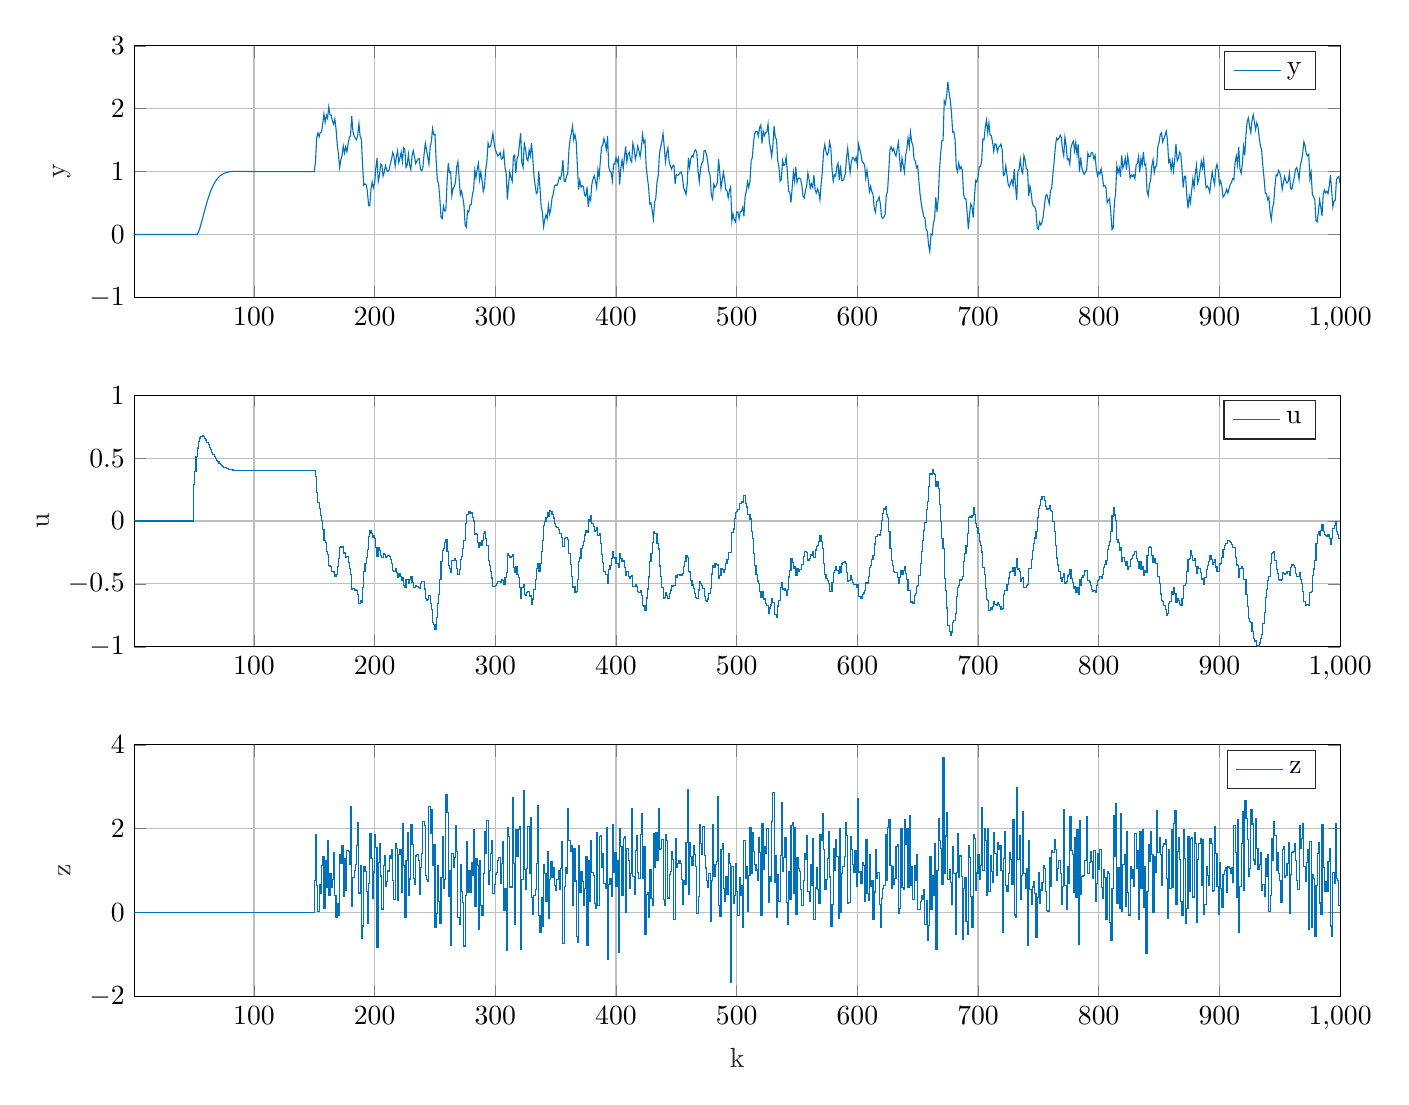
\begin{tikzpicture}

\begin{axis}[%
width=6.028in,
height=1.258in,
at={(1.011in,4.137in)},
scale only axis,
xmin=1,
xmax=1000,
ymin=-1,
ymax=3,
ylabel style={font=\color{white!15!black}},
ylabel={y},
axis background/.style={fill=white},
xmajorgrids,
ymajorgrids,
legend style={legend cell align=left, align=left, draw=white!15!black}
]
\addplot [color=mycolor1]
  table[row sep=crcr]{%
1	0\\
2	0\\
3	0\\
4	0\\
5	0\\
6	0\\
7	0\\
8	0\\
9	0\\
10	0\\
11	0\\
12	0\\
13	0\\
14	0\\
15	0\\
16	0\\
17	0\\
18	0\\
19	0\\
20	0\\
21	0\\
22	0\\
23	0\\
24	0\\
25	0\\
26	0\\
27	0\\
28	0\\
29	0\\
30	0\\
31	0\\
32	0\\
33	0\\
34	0\\
35	0\\
36	0\\
37	0\\
38	0\\
39	0\\
40	0\\
41	0\\
42	0\\
43	0\\
44	0\\
45	0\\
46	0\\
47	0\\
48	0\\
49	0\\
50	0\\
51	0\\
52	0\\
53	0\\
54	0.039119\\
55	0.090032\\
56	0.15448\\
57	0.22449\\
58	0.29764\\
59	0.37063\\
60	0.44164\\
61	0.50914\\
62	0.57223\\
63	0.63032\\
64	0.68313\\
65	0.73061\\
66	0.77286\\
67	0.81011\\
68	0.84266\\
69	0.87086\\
70	0.8951\\
71	0.91576\\
72	0.93322\\
73	0.94786\\
74	0.96003\\
75	0.97004\\
76	0.97821\\
77	0.98479\\
78	0.99003\\
79	0.99414\\
80	0.99731\\
81	0.99971\\
82	1.0015\\
83	1.0027\\
84	1.0036\\
85	1.0041\\
86	1.0043\\
87	1.0044\\
88	1.0043\\
89	1.0042\\
90	1.0039\\
91	1.0036\\
92	1.0033\\
93	1.003\\
94	1.0027\\
95	1.0024\\
96	1.0021\\
97	1.0018\\
98	1.0016\\
99	1.0013\\
100	1.0011\\
101	1.001\\
102	1.0008\\
103	1.0007\\
104	1.0005\\
105	1.0004\\
106	1.0003\\
107	1.0003\\
108	1.0002\\
109	1.0002\\
110	1.0001\\
111	1.0001\\
112	1.0001\\
113	1\\
114	1\\
115	1\\
116	1\\
117	0.99999\\
118	0.99998\\
119	0.99998\\
120	0.99998\\
121	0.99998\\
122	0.99998\\
123	0.99998\\
124	0.99998\\
125	0.99998\\
126	0.99998\\
127	0.99998\\
128	0.99998\\
129	0.99998\\
130	0.99998\\
131	0.99998\\
132	0.99999\\
133	0.99999\\
134	0.99999\\
135	0.99999\\
136	0.99999\\
137	0.99999\\
138	0.99999\\
139	0.99999\\
140	0.99999\\
141	0.99999\\
142	0.99999\\
143	0.99999\\
144	0.99999\\
145	0.99999\\
146	0.99999\\
147	0.99999\\
148	0.99999\\
149	0.99999\\
150	0.99999\\
151	1.1618\\
152	1.5401\\
153	1.6154\\
154	1.5532\\
155	1.6277\\
156	1.6284\\
157	1.7623\\
158	1.919\\
159	1.7823\\
160	1.8962\\
161	1.847\\
162	2.0307\\
163	1.9082\\
164	1.8965\\
165	1.8074\\
166	1.7547\\
167	1.8357\\
168	1.6833\\
169	1.4336\\
170	1.2755\\
171	1.0642\\
172	1.1861\\
173	1.2525\\
174	1.4079\\
175	1.2966\\
176	1.3894\\
177	1.3128\\
178	1.439\\
179	1.544\\
180	1.5664\\
181	1.8803\\
182	1.6414\\
183	1.5659\\
184	1.5285\\
185	1.5073\\
186	1.5815\\
187	1.76\\
188	1.5578\\
189	1.5167\\
190	1.1019\\
191	0.78362\\
192	0.80473\\
193	0.79296\\
194	0.69231\\
195	0.45678\\
196	0.45911\\
197	0.72028\\
198	0.83472\\
199	0.74707\\
200	0.81345\\
201	1.0619\\
202	1.213\\
203	0.84291\\
204	0.94317\\
205	1.1187\\
206	1.1027\\
207	0.92931\\
208	0.99462\\
209	1.0963\\
210	1.0286\\
211	0.99954\\
212	1.0246\\
213	1.121\\
214	1.1927\\
215	1.3048\\
216	1.2445\\
217	1.0896\\
218	1.2332\\
219	1.3288\\
220	1.1438\\
221	1.2193\\
222	1.3064\\
223	1.1577\\
224	1.3771\\
225	1.3564\\
226	1.0693\\
227	1.1077\\
228	1.2743\\
229	1.0996\\
230	1.032\\
231	1.2472\\
232	1.3339\\
233	1.2382\\
234	1.1264\\
235	1.1659\\
236	1.2024\\
237	1.2049\\
238	1.0336\\
239	1.0148\\
240	1.0689\\
241	1.278\\
242	1.4497\\
243	1.348\\
244	1.2348\\
245	1.1185\\
246	1.3867\\
247	1.4802\\
248	1.6858\\
249	1.5859\\
250	1.5932\\
251	1.1738\\
252	0.85558\\
253	0.80985\\
254	0.57966\\
255	0.27615\\
256	0.25086\\
257	0.45013\\
258	0.37447\\
259	0.37727\\
260	0.82452\\
261	1.1321\\
262	0.9886\\
263	1.0015\\
264	0.618\\
265	0.73255\\
266	0.76196\\
267	0.83267\\
268	1.0739\\
269	1.1567\\
270	0.89581\\
271	0.62753\\
272	0.689\\
273	0.59835\\
274	0.4698\\
275	0.14469\\
276	0.11804\\
277	0.37437\\
278	0.35496\\
279	0.46871\\
280	0.47485\\
281	0.63033\\
282	0.71338\\
283	1.0204\\
284	0.90305\\
285	1.0428\\
286	1.1289\\
287	0.86909\\
288	0.99118\\
289	0.85838\\
290	0.68557\\
291	0.75367\\
292	1.025\\
293	1.1564\\
294	1.4528\\
295	1.3908\\
296	1.4012\\
297	1.4894\\
298	1.6147\\
299	1.4535\\
300	1.348\\
301	1.2992\\
302	1.2507\\
303	1.2701\\
304	1.3019\\
305	1.1981\\
306	1.2064\\
307	1.3248\\
308	1.0735\\
309	0.96759\\
310	0.5564\\
311	0.80788\\
312	0.99137\\
313	0.90317\\
314	0.84483\\
315	1.2448\\
316	1.2627\\
317	0.97498\\
318	1.2042\\
319	1.2564\\
320	1.4348\\
321	1.6118\\
322	1.1356\\
323	1.0672\\
324	1.446\\
325	1.366\\
326	1.2047\\
327	1.1714\\
328	1.3401\\
329	1.2504\\
330	1.4539\\
331	1.2302\\
332	0.93875\\
333	0.77715\\
334	0.65262\\
335	0.67765\\
336	1.0024\\
337	0.74609\\
338	0.44214\\
339	0.35436\\
340	0.12453\\
341	0.24113\\
342	0.3138\\
343	0.25163\\
344	0.46704\\
345	0.32539\\
346	0.40735\\
347	0.57734\\
348	0.64514\\
349	0.76579\\
350	0.78625\\
351	0.77783\\
352	0.82271\\
353	0.90844\\
354	0.88468\\
355	0.97266\\
356	1.1836\\
357	0.84948\\
358	0.84233\\
359	0.92976\\
360	0.97138\\
361	1.3466\\
362	1.5166\\
363	1.611\\
364	1.7225\\
365	1.5055\\
366	1.5882\\
367	1.4828\\
368	1.0936\\
369	0.71356\\
370	0.86176\\
371	0.75409\\
372	0.77587\\
373	0.75963\\
374	0.62861\\
375	0.60818\\
376	0.75606\\
377	0.43877\\
378	0.60014\\
379	0.54216\\
380	0.80075\\
381	0.88049\\
382	0.93464\\
383	0.85074\\
384	0.74397\\
385	1.0316\\
386	0.91109\\
387	1.1607\\
388	1.3906\\
389	1.4228\\
390	1.5254\\
391	1.452\\
392	1.3531\\
393	1.5659\\
394	1.0727\\
395	1.0104\\
396	0.9841\\
397	0.85478\\
398	1.1219\\
399	1.1188\\
400	1.2203\\
401	1.1482\\
402	1.2104\\
403	0.7937\\
404	1.0464\\
405	1.1831\\
406	1.0509\\
407	1.2344\\
408	1.4018\\
409	1.1602\\
410	1.2759\\
411	1.3069\\
412	1.1837\\
413	1.1526\\
414	1.4509\\
415	1.3644\\
416	1.1981\\
417	1.2749\\
418	1.4054\\
419	1.3318\\
420	1.2381\\
421	1.3748\\
422	1.5924\\
423	1.4571\\
424	1.4993\\
425	1.0837\\
426	0.90555\\
427	0.7529\\
428	0.4855\\
429	0.50309\\
430	0.37701\\
431	0.24495\\
432	0.50954\\
433	0.57985\\
434	0.83549\\
435	0.93331\\
436	1.2852\\
437	1.389\\
438	1.4789\\
439	1.6025\\
440	1.3864\\
441	1.1528\\
442	1.2954\\
443	1.3795\\
444	1.1599\\
445	1.0903\\
446	1.0396\\
447	1.0913\\
448	1.1007\\
449	0.80245\\
450	0.95397\\
451	0.94159\\
452	0.94788\\
453	0.98254\\
454	0.99421\\
455	0.92606\\
456	0.7418\\
457	0.69799\\
458	0.6376\\
459	0.79925\\
460	1.2195\\
461	1.069\\
462	1.206\\
463	1.256\\
464	1.2389\\
465	1.3254\\
466	1.3455\\
467	1.2974\\
468	1.0106\\
469	0.83649\\
470	1.0462\\
471	1.1303\\
472	1.1559\\
473	1.3329\\
474	1.338\\
475	1.2769\\
476	1.1548\\
477	1.0017\\
478	0.934\\
479	0.62715\\
480	0.56508\\
481	0.79825\\
482	0.74682\\
483	0.77542\\
484	0.82707\\
485	1.2007\\
486	0.98305\\
487	0.73719\\
488	0.86072\\
489	0.98749\\
490	0.87076\\
491	0.71058\\
492	0.69266\\
493	0.58464\\
494	0.69885\\
495	0.75697\\
496	0.21101\\
497	0.32471\\
498	0.23743\\
499	0.20137\\
500	0.35829\\
501	0.35998\\
502	0.25299\\
503	0.36222\\
504	0.36934\\
505	0.43466\\
506	0.2894\\
507	0.60256\\
508	0.69392\\
509	0.83686\\
510	0.74889\\
511	0.84374\\
512	1.1727\\
513	1.2254\\
514	1.4802\\
515	1.6075\\
516	1.6416\\
517	1.6373\\
518	1.5658\\
519	1.7044\\
520	1.741\\
521	1.4453\\
522	1.6421\\
523	1.573\\
524	1.6217\\
525	1.6305\\
526	1.7551\\
527	1.487\\
528	1.371\\
529	1.2418\\
530	1.4199\\
531	1.7254\\
532	1.5398\\
533	1.5161\\
534	1.1746\\
535	1.0748\\
536	0.84588\\
537	0.87471\\
538	1.1758\\
539	1.0972\\
540	1.1119\\
541	1.232\\
542	1.0014\\
543	0.68451\\
544	0.66861\\
545	0.50775\\
546	0.74774\\
547	0.98802\\
548	0.84913\\
549	1.0737\\
550	0.82728\\
551	0.89307\\
552	0.8984\\
553	0.87974\\
554	0.77937\\
555	0.60838\\
556	0.58222\\
557	0.69883\\
558	0.77635\\
559	0.97648\\
560	0.87625\\
561	0.73863\\
562	0.80478\\
563	0.75106\\
564	0.94249\\
565	0.70842\\
566	0.66066\\
567	0.72658\\
568	0.66756\\
569	0.55255\\
570	0.8061\\
571	1.0031\\
572	1.3202\\
573	1.4295\\
574	1.3187\\
575	1.2614\\
576	1.3031\\
577	1.4679\\
578	1.3757\\
579	1.0371\\
580	0.84657\\
581	0.94975\\
582	0.92953\\
583	1.0786\\
584	1.1344\\
585	0.87109\\
586	1.0964\\
587	0.86477\\
588	0.85564\\
589	0.89158\\
590	0.96635\\
591	1.2158\\
592	1.3713\\
593	1.1645\\
594	0.9838\\
595	1.1519\\
596	1.2236\\
597	1.2116\\
598	1.1671\\
599	1.2316\\
600	1.1043\\
601	1.4347\\
602	1.353\\
603	1.2783\\
604	1.1566\\
605	1.1383\\
606	1.1044\\
607	0.89264\\
608	1.0207\\
609	0.85995\\
610	0.68375\\
611	0.76722\\
612	0.67874\\
613	0.63817\\
614	0.4126\\
615	0.35514\\
616	0.52686\\
617	0.54054\\
618	0.59603\\
619	0.49326\\
620	0.28754\\
621	0.25452\\
622	0.27731\\
623	0.32157\\
624	0.62961\\
625	0.68026\\
626	1.0065\\
627	1.3395\\
628	1.3962\\
629	1.3299\\
630	1.3666\\
631	1.292\\
632	1.247\\
633	1.3605\\
634	1.4651\\
635	1.2035\\
636	0.99741\\
637	1.2142\\
638	1.0994\\
639	0.99202\\
640	1.2571\\
641	1.3612\\
642	1.5355\\
643	1.3943\\
644	1.6272\\
645	1.4723\\
646	1.4184\\
647	1.2021\\
648	1.1683\\
649	1.0608\\
650	1.0904\\
651	0.84718\\
652	0.63196\\
653	0.48489\\
654	0.3833\\
655	0.28689\\
656	0.26431\\
657	0.079235\\
658	0.049356\\
659	-0.16641\\
660	-0.27047\\
661	0.0050443\\
662	-0.0067432\\
663	0.1763\\
664	0.25348\\
665	0.59031\\
666	0.36148\\
667	0.56208\\
668	1.0054\\
669	1.2799\\
670	1.4923\\
671	1.4919\\
672	2.1246\\
673	2.0755\\
674	2.2066\\
675	2.4285\\
676	2.2531\\
677	2.1318\\
678	1.9352\\
679	1.6258\\
680	1.6367\\
681	1.4985\\
682	1.0646\\
683	0.99992\\
684	1.1367\\
685	1.0401\\
686	1.0773\\
687	1.0149\\
688	0.64111\\
689	0.57227\\
690	0.56563\\
691	0.33996\\
692	0.087971\\
693	0.32724\\
694	0.48641\\
695	0.44332\\
696	0.26741\\
697	0.58944\\
698	0.85753\\
699	0.83486\\
700	0.91552\\
701	1.0766\\
702	1.0856\\
703	1.1629\\
704	1.5195\\
705	1.5077\\
706	1.7091\\
707	1.8203\\
708	1.6195\\
709	1.7761\\
710	1.5778\\
711	1.5678\\
712	1.4746\\
713	1.3232\\
714	1.4419\\
715	1.4364\\
716	1.3179\\
717	1.3863\\
718	1.4068\\
719	1.4394\\
720	1.3432\\
721	0.93619\\
722	0.94779\\
723	1.0933\\
724	0.94526\\
725	0.79613\\
726	0.75821\\
727	0.82966\\
728	0.86702\\
729	0.77839\\
730	1.0369\\
731	0.78237\\
732	0.54621\\
733	1.0028\\
734	1.0348\\
735	1.1926\\
736	1.0191\\
737	0.97393\\
738	1.2564\\
739	1.1854\\
740	1.0494\\
741	1.0286\\
742	0.61034\\
743	0.7701\\
744	0.6632\\
745	0.49493\\
746	0.45084\\
747	0.44046\\
748	0.37772\\
749	0.10885\\
750	0.084695\\
751	0.19638\\
752	0.15042\\
753	0.19566\\
754	0.28753\\
755	0.46126\\
756	0.61226\\
757	0.63577\\
758	0.5638\\
759	0.49043\\
760	0.69871\\
761	0.73498\\
762	0.95556\\
763	1.1461\\
764	1.379\\
765	1.5335\\
766	1.5055\\
767	1.5318\\
768	1.5795\\
769	1.543\\
770	1.3445\\
771	1.2507\\
772	1.5473\\
773	1.4229\\
774	1.1898\\
775	1.2049\\
776	1.1187\\
777	1.3805\\
778	1.4447\\
779	1.4848\\
780	1.3296\\
781	1.4618\\
782	1.2687\\
783	1.4334\\
784	0.99507\\
785	1.2269\\
786	1.0623\\
787	0.99594\\
788	0.95783\\
789	0.99448\\
790	1.0307\\
791	1.2911\\
792	1.2365\\
793	1.2454\\
794	1.3058\\
795	1.2977\\
796	1.2017\\
797	1.2559\\
798	1.0388\\
799	0.93428\\
800	0.99393\\
801	0.96195\\
802	1.0444\\
803	0.92646\\
804	0.76925\\
805	0.77821\\
806	0.74322\\
807	0.50466\\
808	0.5423\\
809	0.57114\\
810	0.35164\\
811	0.077797\\
812	0.1062\\
813	0.50495\\
814	0.66602\\
815	1.097\\
816	0.98197\\
817	1.0577\\
818	0.91664\\
819	1.2559\\
820	1.0567\\
821	1.1101\\
822	1.2133\\
823	1.0282\\
824	1.2455\\
825	1.1222\\
826	0.89524\\
827	0.94389\\
828	0.91986\\
829	0.94659\\
830	0.88945\\
831	1.1067\\
832	1.1293\\
833	1.2401\\
834	0.98796\\
835	1.2068\\
836	1.1063\\
837	1.3114\\
838	1.1057\\
839	1.1179\\
840	0.6914\\
841	0.6165\\
842	0.79496\\
843	0.86269\\
844	1.0926\\
845	1.1897\\
846	0.98391\\
847	1.0869\\
848	1.0895\\
849	1.3996\\
850	1.4612\\
851	1.5892\\
852	1.6172\\
853	1.4692\\
854	1.5273\\
855	1.5786\\
856	1.639\\
857	1.491\\
858	1.1496\\
859	1.191\\
860	1.0217\\
861	1.1678\\
862	1.0131\\
863	1.1994\\
864	1.4399\\
865	1.1737\\
866	1.2111\\
867	1.3098\\
868	1.2761\\
869	1.0339\\
870	0.74493\\
871	0.92083\\
872	0.92873\\
873	0.60952\\
874	0.41631\\
875	0.61103\\
876	0.5064\\
877	0.69806\\
878	0.88363\\
879	0.74979\\
880	0.9679\\
881	1.1015\\
882	0.81743\\
883	0.88676\\
884	1.0246\\
885	1.1625\\
886	1.056\\
887	1.1952\\
888	0.93243\\
889	0.74339\\
890	0.77077\\
891	0.73791\\
892	0.66812\\
893	0.8502\\
894	0.99256\\
895	0.88331\\
896	0.79577\\
897	1.0395\\
898	1.1178\\
899	1.0195\\
900	0.79574\\
901	0.8518\\
902	0.76757\\
903	0.59454\\
904	0.6188\\
905	0.65904\\
906	0.71934\\
907	0.65595\\
908	0.73187\\
909	0.79389\\
910	0.82625\\
911	0.89027\\
912	0.87058\\
913	1.1428\\
914	1.2491\\
915	1.1117\\
916	1.3883\\
917	1.0467\\
918	0.97012\\
919	1.1198\\
920	1.4017\\
921	1.2583\\
922	1.5905\\
923	1.7917\\
924	1.8539\\
925	1.7175\\
926	1.6185\\
927	1.815\\
928	1.9029\\
929	1.7917\\
930	1.6669\\
931	1.7772\\
932	1.71\\
933	1.5392\\
934	1.4086\\
935	1.3443\\
936	1.0904\\
937	0.89323\\
938	0.65987\\
939	0.64642\\
940	0.55338\\
941	0.59313\\
942	0.35504\\
943	0.23525\\
944	0.43004\\
945	0.49498\\
946	0.76581\\
947	0.95046\\
948	0.93587\\
949	1.0177\\
950	0.98088\\
951	0.90159\\
952	0.71648\\
953	0.81793\\
954	0.92092\\
955	0.85489\\
956	0.8175\\
957	0.8448\\
958	0.97238\\
959	0.73115\\
960	0.71635\\
961	0.81744\\
962	0.90603\\
963	1.0324\\
964	1.0644\\
965	0.99066\\
966	0.87696\\
967	1.0961\\
968	1.172\\
969	1.2886\\
970	1.4728\\
971	1.4135\\
972	1.2817\\
973	1.2502\\
974	1.2767\\
975	0.886\\
976	0.98758\\
977	0.64077\\
978	0.59934\\
979	0.55548\\
980	0.22308\\
981	0.19961\\
982	0.34931\\
983	0.54975\\
984	0.4399\\
985	0.29645\\
986	0.62991\\
987	0.70776\\
988	0.66319\\
989	0.68613\\
990	0.64875\\
991	0.76922\\
992	0.9429\\
993	0.70254\\
994	0.43955\\
995	0.53128\\
996	0.54788\\
997	0.87648\\
998	0.90323\\
999	0.92103\\
1000	0.81268\\
};
\addlegendentry{y}

\end{axis}

\begin{axis}[%
width=6.028in,
height=1.258in,
at={(1.011in,2.39in)},
scale only axis,
xmin=1,
xmax=1000,
ymin=-1,
ymax=1,
ylabel style={font=\color{white!15!black}},
ylabel={u},
axis background/.style={fill=white},
xmajorgrids,
ymajorgrids,
legend style={legend cell align=left, align=left, draw=white!15!black}
]
\addplot[const plot, color=mycolor1] table[row sep=crcr] {%
1	0\\
2	0\\
3	0\\
4	0\\
5	0\\
6	0\\
7	0\\
8	0\\
9	0\\
10	0\\
11	0\\
12	0\\
13	0\\
14	0\\
15	0\\
16	0\\
17	0\\
18	0\\
19	0\\
20	0\\
21	0\\
22	0\\
23	0\\
24	0\\
25	0\\
26	0\\
27	0\\
28	0\\
29	0\\
30	0\\
31	0\\
32	0\\
33	0\\
34	0\\
35	0\\
36	0\\
37	0\\
38	0\\
39	0\\
40	0\\
41	0\\
42	0\\
43	0\\
44	0\\
45	0\\
46	0\\
47	0\\
48	0\\
49	0\\
50	0.28956\\
51	0.39251\\
52	0.5131\\
53	0.58007\\
54	0.63135\\
55	0.65951\\
56	0.67407\\
57	0.67664\\
58	0.67103\\
59	0.65931\\
60	0.64358\\
61	0.62529\\
62	0.60567\\
63	0.58562\\
64	0.56581\\
65	0.54674\\
66	0.52873\\
67	0.512\\
68	0.49669\\
69	0.48283\\
70	0.47042\\
71	0.45942\\
72	0.44977\\
73	0.44136\\
74	0.4341\\
75	0.42788\\
76	0.4226\\
77	0.41815\\
78	0.41444\\
79	0.41136\\
80	0.40884\\
81	0.4068\\
82	0.40516\\
83	0.40387\\
84	0.40286\\
85	0.40209\\
86	0.40151\\
87	0.4011\\
88	0.40081\\
89	0.40063\\
90	0.40052\\
91	0.40048\\
92	0.40048\\
93	0.40051\\
94	0.40057\\
95	0.40065\\
96	0.40073\\
97	0.40082\\
98	0.40091\\
99	0.401\\
100	0.40108\\
101	0.40116\\
102	0.40123\\
103	0.4013\\
104	0.40136\\
105	0.40142\\
106	0.40146\\
107	0.4015\\
108	0.40154\\
109	0.40157\\
110	0.4016\\
111	0.40162\\
112	0.40164\\
113	0.40166\\
114	0.40167\\
115	0.40168\\
116	0.40169\\
117	0.4017\\
118	0.4017\\
119	0.40171\\
120	0.40171\\
121	0.40171\\
122	0.40171\\
123	0.40172\\
124	0.40172\\
125	0.40172\\
126	0.40172\\
127	0.40172\\
128	0.40172\\
129	0.40172\\
130	0.40172\\
131	0.40172\\
132	0.40172\\
133	0.40171\\
134	0.40171\\
135	0.40171\\
136	0.40171\\
137	0.40171\\
138	0.40171\\
139	0.40171\\
140	0.40171\\
141	0.40171\\
142	0.40171\\
143	0.40171\\
144	0.40171\\
145	0.40171\\
146	0.40171\\
147	0.40171\\
148	0.40171\\
149	0.40171\\
150	0.40171\\
151	0.35486\\
152	0.22866\\
153	0.14839\\
154	0.10219\\
155	0.042484\\
156	0.0057956\\
157	-0.067326\\
158	-0.15373\\
159	-0.17183\\
160	-0.24171\\
161	-0.26385\\
162	-0.35411\\
163	-0.36496\\
164	-0.40125\\
165	-0.3997\\
166	-0.40549\\
167	-0.44074\\
168	-0.4219\\
169	-0.36342\\
170	-0.30066\\
171	-0.21072\\
172	-0.20622\\
173	-0.20653\\
174	-0.25797\\
175	-0.24793\\
176	-0.28956\\
177	-0.28147\\
178	-0.33153\\
179	-0.38022\\
180	-0.42301\\
181	-0.54618\\
182	-0.53696\\
183	-0.55214\\
184	-0.54761\\
185	-0.55263\\
186	-0.58187\\
187	-0.65294\\
188	-0.63504\\
189	-0.64348\\
190	-0.5267\\
191	-0.40381\\
192	-0.33938\\
193	-0.28673\\
194	-0.22686\\
195	-0.12489\\
196	-0.073115\\
197	-0.10099\\
198	-0.12893\\
199	-0.11852\\
200	-0.13668\\
201	-0.20744\\
202	-0.27853\\
203	-0.21346\\
204	-0.23579\\
205	-0.27308\\
206	-0.28979\\
207	-0.25486\\
208	-0.26494\\
209	-0.28777\\
210	-0.28051\\
211	-0.27577\\
212	-0.27883\\
213	-0.30713\\
214	-0.33929\\
215	-0.39157\\
216	-0.40173\\
217	-0.37586\\
218	-0.4116\\
219	-0.44671\\
220	-0.41902\\
221	-0.44236\\
222	-0.46962\\
223	-0.44662\\
224	-0.51173\\
225	-0.52434\\
226	-0.46811\\
227	-0.46403\\
228	-0.49791\\
229	-0.463\\
230	-0.44328\\
231	-0.48993\\
232	-0.52931\\
233	-0.53139\\
234	-0.5116\\
235	-0.51804\\
236	-0.52805\\
237	-0.53738\\
238	-0.4961\\
239	-0.48075\\
240	-0.48113\\
241	-0.54059\\
242	-0.61328\\
243	-0.62796\\
244	-0.62127\\
245	-0.59019\\
246	-0.65805\\
247	-0.70399\\
248	-0.80344\\
249	-0.82432\\
250	-0.86548\\
251	-0.76721\\
252	-0.65786\\
253	-0.58272\\
254	-0.4664\\
255	-0.32198\\
256	-0.23305\\
257	-0.21992\\
258	-0.16839\\
259	-0.14399\\
260	-0.24375\\
261	-0.3559\\
262	-0.37664\\
263	-0.41114\\
264	-0.31142\\
265	-0.31653\\
266	-0.2956\\
267	-0.31123\\
268	-0.37762\\
269	-0.42758\\
270	-0.38586\\
271	-0.30411\\
272	-0.27883\\
273	-0.22085\\
274	-0.1566\\
275	-0.020969\\
276	0.055169\\
277	0.049821\\
278	0.077768\\
279	0.059038\\
280	0.067296\\
281	0.027142\\
282	-0.00035564\\
283	-0.10359\\
284	-0.10649\\
285	-0.17154\\
286	-0.21346\\
287	-0.16934\\
288	-0.19748\\
289	-0.15446\\
290	-0.098133\\
291	-0.083858\\
292	-0.14156\\
293	-0.19595\\
294	-0.31589\\
295	-0.35281\\
296	-0.40152\\
297	-0.45275\\
298	-0.52315\\
299	-0.51848\\
300	-0.50961\\
301	-0.4943\\
302	-0.47827\\
303	-0.47942\\
304	-0.48974\\
305	-0.46844\\
306	-0.47013\\
307	-0.50233\\
308	-0.44563\\
309	-0.40719\\
310	-0.26031\\
311	-0.27432\\
312	-0.29271\\
313	-0.2819\\
314	-0.26438\\
315	-0.36899\\
316	-0.40551\\
317	-0.36471\\
318	-0.42362\\
319	-0.44786\\
320	-0.52746\\
321	-0.61342\\
322	-0.53038\\
323	-0.5065\\
324	-0.5855\\
325	-0.59031\\
326	-0.57188\\
327	-0.55803\\
328	-0.60051\\
329	-0.58989\\
330	-0.66092\\
331	-0.62031\\
332	-0.54584\\
333	-0.46251\\
334	-0.38044\\
335	-0.33916\\
336	-0.39804\\
337	-0.33429\\
338	-0.23972\\
339	-0.15849\\
340	-0.035698\\
341	-0.0016982\\
342	0.027556\\
343	0.069011\\
344	0.037007\\
345	0.086173\\
346	0.078063\\
347	0.049499\\
348	0.023905\\
349	-0.020136\\
350	-0.041061\\
351	-0.051798\\
352	-0.068146\\
353	-0.097024\\
354	-0.10115\\
355	-0.13277\\
356	-0.20287\\
357	-0.13802\\
358	-0.13068\\
359	-0.13201\\
360	-0.14402\\
361	-0.25646\\
362	-0.34802\\
363	-0.43925\\
364	-0.52758\\
365	-0.52237\\
366	-0.57165\\
367	-0.56043\\
368	-0.46468\\
369	-0.32247\\
370	-0.29404\\
371	-0.2196\\
372	-0.19793\\
373	-0.1653\\
374	-0.11115\\
375	-0.075621\\
376	-0.089051\\
377	0.009547\\
378	-0.0034786\\
379	0.041337\\
380	-0.020031\\
381	-0.046545\\
382	-0.085747\\
383	-0.076603\\
384	-0.049549\\
385	-0.11681\\
386	-0.096116\\
387	-0.17898\\
388	-0.26512\\
389	-0.32849\\
390	-0.40265\\
391	-0.42478\\
392	-0.42634\\
393	-0.49671\\
394	-0.38352\\
395	-0.3504\\
396	-0.30134\\
397	-0.24484\\
398	-0.29167\\
399	-0.29431\\
400	-0.34051\\
401	-0.33587\\
402	-0.36648\\
403	-0.25536\\
404	-0.29981\\
405	-0.32397\\
406	-0.31154\\
407	-0.36616\\
408	-0.43063\\
409	-0.40085\\
410	-0.44219\\
411	-0.45784\\
412	-0.44341\\
413	-0.43534\\
414	-0.51736\\
415	-0.52262\\
416	-0.50304\\
417	-0.5206\\
418	-0.56281\\
419	-0.56583\\
420	-0.55491\\
421	-0.59405\\
422	-0.67184\\
423	-0.67583\\
424	-0.71473\\
425	-0.61192\\
426	-0.54045\\
427	-0.44548\\
428	-0.32136\\
429	-0.25955\\
430	-0.16867\\
431	-0.082366\\
432	-0.10036\\
433	-0.099995\\
434	-0.17529\\
435	-0.22292\\
436	-0.35736\\
437	-0.44159\\
438	-0.53154\\
439	-0.61819\\
440	-0.61082\\
441	-0.56562\\
442	-0.59041\\
443	-0.61563\\
444	-0.57367\\
445	-0.54885\\
446	-0.51641\\
447	-0.51756\\
448	-0.51474\\
449	-0.43068\\
450	-0.44536\\
451	-0.42415\\
452	-0.4257\\
453	-0.4294\\
454	-0.43485\\
455	-0.41756\\
456	-0.35908\\
457	-0.3201\\
458	-0.27188\\
459	-0.29082\\
460	-0.40429\\
461	-0.40508\\
462	-0.47428\\
463	-0.50861\\
464	-0.53564\\
465	-0.57862\\
466	-0.60804\\
467	-0.61831\\
468	-0.54886\\
469	-0.47915\\
470	-0.49818\\
471	-0.51393\\
472	-0.53571\\
473	-0.59925\\
474	-0.63004\\
475	-0.64229\\
476	-0.62035\\
477	-0.57377\\
478	-0.53407\\
479	-0.4212\\
480	-0.35506\\
481	-0.36858\\
482	-0.34214\\
483	-0.34453\\
484	-0.34941\\
485	-0.458\\
486	-0.432\\
487	-0.38022\\
488	-0.38538\\
489	-0.40926\\
490	-0.3858\\
491	-0.33622\\
492	-0.30462\\
493	-0.24726\\
494	-0.25041\\
495	-0.25006\\
496	-0.091103\\
497	-0.063525\\
498	0.021195\\
499	0.069955\\
500	0.072284\\
501	0.091696\\
502	0.13726\\
503	0.13596\\
504	0.15439\\
505	0.14882\\
506	0.20283\\
507	0.13746\\
508	0.11155\\
509	0.048376\\
510	0.053336\\
511	0.016218\\
512	-0.084025\\
513	-0.14184\\
514	-0.26069\\
515	-0.35171\\
516	-0.4266\\
517	-0.47654\\
518	-0.49641\\
519	-0.56122\\
520	-0.60553\\
521	-0.56063\\
522	-0.61983\\
523	-0.61455\\
524	-0.65292\\
525	-0.67311\\
526	-0.73518\\
527	-0.69175\\
528	-0.66777\\
529	-0.61546\\
530	-0.65067\\
531	-0.74392\\
532	-0.74069\\
533	-0.76377\\
534	-0.67546\\
535	-0.62873\\
536	-0.52611\\
537	-0.49267\\
538	-0.54346\\
539	-0.53426\\
540	-0.55155\\
541	-0.58898\\
542	-0.54191\\
543	-0.44486\\
544	-0.39259\\
545	-0.30216\\
546	-0.32714\\
547	-0.37927\\
548	-0.36448\\
549	-0.43501\\
550	-0.38026\\
551	-0.39868\\
552	-0.38737\\
553	-0.3838\\
554	-0.34817\\
555	-0.28399\\
556	-0.24198\\
557	-0.24155\\
558	-0.25094\\
559	-0.30974\\
560	-0.30048\\
561	-0.27053\\
562	-0.27189\\
563	-0.2464\\
564	-0.29176\\
565	-0.23019\\
566	-0.20579\\
567	-0.19472\\
568	-0.16618\\
569	-0.11719\\
570	-0.16197\\
571	-0.21807\\
572	-0.34017\\
573	-0.4262\\
574	-0.45574\\
575	-0.47022\\
576	-0.49492\\
577	-0.55736\\
578	-0.56257\\
579	-0.48696\\
580	-0.40845\\
581	-0.39277\\
582	-0.36433\\
583	-0.39689\\
584	-0.41747\\
585	-0.35894\\
586	-0.40849\\
587	-0.34214\\
588	-0.33231\\
589	-0.31863\\
590	-0.33455\\
591	-0.40794\\
592	-0.48308\\
593	-0.46977\\
594	-0.43231\\
595	-0.46311\\
596	-0.4865\\
597	-0.50291\\
598	-0.50303\\
599	-0.52765\\
600	-0.50122\\
601	-0.59686\\
602	-0.60113\\
603	-0.61176\\
604	-0.58146\\
605	-0.57201\\
606	-0.55337\\
607	-0.48687\\
608	-0.49785\\
609	-0.4387\\
610	-0.37306\\
611	-0.35698\\
612	-0.30843\\
613	-0.27548\\
614	-0.18281\\
615	-0.12252\\
616	-0.12161\\
617	-0.10612\\
618	-0.11243\\
619	-0.074318\\
620	0.0024724\\
621	0.056331\\
622	0.095764\\
623	0.11691\\
624	0.052696\\
625	0.02835\\
626	-0.085642\\
627	-0.22019\\
628	-0.31062\\
629	-0.35473\\
630	-0.40163\\
631	-0.40763\\
632	-0.41122\\
633	-0.44871\\
634	-0.49662\\
635	-0.45203\\
636	-0.39287\\
637	-0.4245\\
638	-0.39083\\
639	-0.36152\\
640	-0.41951\\
641	-0.46499\\
642	-0.55079\\
643	-0.55349\\
644	-0.64804\\
645	-0.63887\\
646	-0.65191\\
647	-0.59373\\
648	-0.57328\\
649	-0.5233\\
650	-0.5148\\
651	-0.4313\\
652	-0.34122\\
653	-0.24474\\
654	-0.15846\\
655	-0.073785\\
656	-0.012308\\
657	0.089573\\
658	0.15574\\
659	0.27666\\
660	0.37443\\
661	0.37232\\
662	0.41092\\
663	0.38099\\
664	0.37248\\
665	0.27497\\
666	0.31728\\
667	0.25744\\
668	0.13255\\
669	-0.0015621\\
670	-0.13737\\
671	-0.21522\\
672	-0.45898\\
673	-0.55042\\
674	-0.69193\\
675	-0.83153\\
676	-0.87774\\
677	-0.90627\\
678	-0.88202\\
679	-0.80527\\
680	-0.78783\\
681	-0.73392\\
682	-0.59843\\
683	-0.52682\\
684	-0.51239\\
685	-0.46927\\
686	-0.46682\\
687	-0.4388\\
688	-0.32343\\
689	-0.25606\\
690	-0.1988\\
691	-0.096727\\
692	0.029317\\
693	0.036122\\
694	0.030793\\
695	0.046521\\
696	0.1093\\
697	0.050691\\
698	-0.022757\\
699	-0.053497\\
700	-0.099965\\
701	-0.16424\\
702	-0.19807\\
703	-0.24657\\
704	-0.37311\\
705	-0.427\\
706	-0.5399\\
707	-0.62606\\
708	-0.63343\\
709	-0.70828\\
710	-0.68409\\
711	-0.70178\\
712	-0.67994\\
713	-0.64243\\
714	-0.6643\\
715	-0.66754\\
716	-0.64809\\
717	-0.667\\
718	-0.67961\\
719	-0.70483\\
720	-0.69397\\
721	-0.58417\\
722	-0.54969\\
723	-0.55305\\
724	-0.50817\\
725	-0.45281\\
726	-0.41038\\
727	-0.40213\\
728	-0.39914\\
729	-0.37005\\
730	-0.43222\\
731	-0.37054\\
732	-0.29716\\
733	-0.38196\\
734	-0.40054\\
735	-0.47686\\
736	-0.45409\\
737	-0.45319\\
738	-0.52552\\
739	-0.53142\\
740	-0.51522\\
741	-0.50376\\
742	-0.37529\\
743	-0.37442\\
744	-0.30728\\
745	-0.23784\\
746	-0.17913\\
747	-0.13473\\
748	-0.082139\\
749	0.030358\\
750	0.096919\\
751	0.12564\\
752	0.1728\\
753	0.19197\\
754	0.19468\\
755	0.15943\\
756	0.11349\\
757	0.089833\\
758	0.098929\\
759	0.12554\\
760	0.084502\\
761	0.072809\\
762	-0.0019224\\
763	-0.080275\\
764	-0.19222\\
765	-0.29369\\
766	-0.35\\
767	-0.40402\\
768	-0.45283\\
769	-0.47764\\
770	-0.44648\\
771	-0.41975\\
772	-0.49261\\
773	-0.48153\\
774	-0.43694\\
775	-0.42519\\
776	-0.38896\\
777	-0.45445\\
778	-0.48998\\
779	-0.53739\\
780	-0.52085\\
781	-0.57004\\
782	-0.53013\\
783	-0.58322\\
784	-0.46699\\
785	-0.51412\\
786	-0.45249\\
787	-0.43227\\
788	-0.39752\\
789	-0.39426\\
790	-0.39561\\
791	-0.47243\\
792	-0.48484\\
793	-0.51442\\
794	-0.54483\\
795	-0.5635\\
796	-0.55262\\
797	-0.57176\\
798	-0.51518\\
799	-0.4738\\
800	-0.4624\\
801	-0.44127\\
802	-0.45689\\
803	-0.42321\\
804	-0.3712\\
805	-0.34531\\
806	-0.31194\\
807	-0.22422\\
808	-0.19341\\
809	-0.16422\\
810	-0.080716\\
811	0.040158\\
812	0.10299\\
813	0.048062\\
814	0.0039392\\
815	-0.14538\\
816	-0.16769\\
817	-0.23241\\
818	-0.21183\\
819	-0.31818\\
820	-0.28876\\
821	-0.32419\\
822	-0.3548\\
823	-0.32395\\
824	-0.38443\\
825	-0.36173\\
826	-0.30772\\
827	-0.29573\\
828	-0.27138\\
829	-0.26958\\
830	-0.24591\\
831	-0.30043\\
832	-0.31911\\
833	-0.37369\\
834	-0.32353\\
835	-0.38479\\
836	-0.36245\\
837	-0.43437\\
838	-0.39327\\
839	-0.40529\\
840	-0.27398\\
841	-0.21255\\
842	-0.20573\\
843	-0.20954\\
844	-0.27576\\
845	-0.32654\\
846	-0.30198\\
847	-0.3345\\
848	-0.33819\\
849	-0.43975\\
850	-0.49412\\
851	-0.58057\\
852	-0.63388\\
853	-0.6367\\
854	-0.67196\\
855	-0.70435\\
856	-0.74955\\
857	-0.73723\\
858	-0.65264\\
859	-0.63658\\
860	-0.56462\\
861	-0.58481\\
862	-0.53101\\
863	-0.5769\\
864	-0.649\\
865	-0.61439\\
866	-0.6341\\
867	-0.66029\\
868	-0.66969\\
869	-0.61264\\
870	-0.51368\\
871	-0.51587\\
872	-0.49458\\
873	-0.39905\\
874	-0.30268\\
875	-0.29733\\
876	-0.23848\\
877	-0.2709\\
878	-0.31487\\
879	-0.29812\\
880	-0.36225\\
881	-0.41378\\
882	-0.36565\\
883	-0.37899\\
884	-0.40684\\
885	-0.46085\\
886	-0.45539\\
887	-0.50763\\
888	-0.44684\\
889	-0.38626\\
890	-0.35435\\
891	-0.31854\\
892	-0.27766\\
893	-0.30497\\
894	-0.34303\\
895	-0.33132\\
896	-0.30925\\
897	-0.36549\\
898	-0.40057\\
899	-0.39972\\
900	-0.34172\\
901	-0.33567\\
902	-0.29237\\
903	-0.22629\\
904	-0.19623\\
905	-0.17768\\
906	-0.17911\\
907	-0.15322\\
908	-0.16309\\
909	-0.17315\\
910	-0.18585\\
911	-0.20766\\
912	-0.20965\\
913	-0.29211\\
914	-0.34962\\
915	-0.35203\\
916	-0.44605\\
917	-0.37992\\
918	-0.36243\\
919	-0.37947\\
920	-0.46623\\
921	-0.46219\\
922	-0.58269\\
923	-0.68209\\
924	-0.77339\\
925	-0.79545\\
926	-0.80407\\
927	-0.87534\\
928	-0.93641\\
929	-0.95463\\
930	-0.94919\\
931	-0.99222\\
932	-0.99583\\
933	-0.96981\\
934	-0.93187\\
935	-0.90147\\
936	-0.81553\\
937	-0.72771\\
938	-0.61128\\
939	-0.54794\\
940	-0.47011\\
941	-0.43957\\
942	-0.33768\\
943	-0.25743\\
944	-0.25286\\
945	-0.24487\\
946	-0.31494\\
947	-0.38399\\
948	-0.41799\\
949	-0.4658\\
950	-0.47579\\
951	-0.46641\\
952	-0.40911\\
953	-0.41398\\
954	-0.42816\\
955	-0.41556\\
956	-0.40208\\
957	-0.39928\\
958	-0.42999\\
959	-0.36878\\
960	-0.34976\\
961	-0.35203\\
962	-0.37304\\
963	-0.4158\\
964	-0.44375\\
965	-0.4419\\
966	-0.41372\\
967	-0.46519\\
968	-0.49706\\
969	-0.55736\\
970	-0.63951\\
971	-0.66864\\
972	-0.66433\\
973	-0.66256\\
974	-0.67138\\
975	-0.56497\\
976	-0.56284\\
977	-0.43409\\
978	-0.38128\\
979	-0.31362\\
980	-0.18157\\
981	-0.1076\\
982	-0.085052\\
983	-0.11238\\
984	-0.078891\\
985	-0.026324\\
986	-0.086383\\
987	-0.10911\\
988	-0.11584\\
989	-0.12267\\
990	-0.1098\\
991	-0.13676\\
992	-0.188\\
993	-0.14032\\
994	-0.057135\\
995	-0.035656\\
996	-0.0072712\\
997	-0.084536\\
998	-0.10722\\
999	-0.1385\\
1000	-0.11807\\
};
\addlegendentry{u}

\end{axis}

\begin{axis}[%
width=6.028in,
height=1.258in,
at={(1.011in,0.642in)},
scale only axis,
xmin=1,
xmax=1000,
xlabel style={font=\color{white!15!black}},
xlabel={k},
ymin=-2,
ymax=4,
ylabel style={font=\color{white!15!black}},
ylabel={z},
axis background/.style={fill=white},
xmajorgrids,
ymajorgrids,
legend style={legend cell align=left, align=left, draw=white!15!black}
]
\addplot[const plot, color=mycolor1] table[row sep=crcr] {%
1	0\\
2	0\\
3	0\\
4	0\\
5	0\\
6	0\\
7	0\\
8	0\\
9	0\\
10	0\\
11	0\\
12	0\\
13	0\\
14	0\\
15	0\\
16	0\\
17	0\\
18	0\\
19	0\\
20	0\\
21	0\\
22	0\\
23	0\\
24	0\\
25	0\\
26	0\\
27	0\\
28	0\\
29	0\\
30	0\\
31	0\\
32	0\\
33	0\\
34	0\\
35	0\\
36	0\\
37	0\\
38	0\\
39	0\\
40	0\\
41	0\\
42	0\\
43	0\\
44	0\\
45	0\\
46	0\\
47	0\\
48	0\\
49	0\\
50	0\\
51	0\\
52	0\\
53	0\\
54	0\\
55	0\\
56	0\\
57	0\\
58	0\\
59	0\\
60	0\\
61	0\\
62	0\\
63	0\\
64	0\\
65	0\\
66	0\\
67	0\\
68	0\\
69	0\\
70	0\\
71	0\\
72	0\\
73	0\\
74	0\\
75	0\\
76	0\\
77	0\\
78	0\\
79	0\\
80	0\\
81	0\\
82	0\\
83	0\\
84	0\\
85	0\\
86	0\\
87	0\\
88	0\\
89	0\\
90	0\\
91	0\\
92	0\\
93	0\\
94	0\\
95	0\\
96	0\\
97	0\\
98	0\\
99	0\\
100	0\\
101	0\\
102	0\\
103	0\\
104	0\\
105	0\\
106	0\\
107	0\\
108	0\\
109	0\\
110	0\\
111	0\\
112	0\\
113	0\\
114	0\\
115	0\\
116	0\\
117	0\\
118	0\\
119	0\\
120	0\\
121	0\\
122	0\\
123	0\\
124	0\\
125	0\\
126	0\\
127	0\\
128	0\\
129	0\\
130	0\\
131	0\\
132	0\\
133	0\\
134	0\\
135	0\\
136	0\\
137	0\\
138	0\\
139	0\\
140	0\\
141	0\\
142	0\\
143	0\\
144	0\\
145	0\\
146	0\\
147	0\\
148	0\\
149	0\\
150	0.75869\\
151	1.8592\\
152	0.63756\\
153	0.032245\\
154	0.67014\\
155	0.44514\\
156	1.1275\\
157	1.3431\\
158	0.097565\\
159	1.2355\\
160	0.59027\\
161	1.7251\\
162	0.41505\\
163	0.93067\\
164	0.59397\\
165	0.79323\\
166	1.4201\\
167	0.41079\\
168	-0.10657\\
169	0.21433\\
170	-0.078141\\
171	1.3799\\
172	1.1631\\
173	1.5894\\
174	0.3744\\
175	1.2766\\
176	0.53735\\
177	1.4869\\
178	1.4546\\
179	1.1556\\
180	2.5373\\
181	0.14909\\
182	0.82879\\
183	1.0051\\
184	1.1499\\
185	1.5958\\
186	2.1467\\
187	0.46688\\
188	1.1311\\
189	-0.61181\\
190	-0.32007\\
191	1.1072\\
192	0.98245\\
193	0.49811\\
194	-0.25762\\
195	0.69576\\
196	1.8775\\
197	1.2872\\
198	0.33129\\
199	0.96722\\
200	1.8648\\
201	1.5493\\
202	-0.82808\\
203	1.1885\\
204	1.6341\\
205	0.87117\\
206	0.083837\\
207	1.1244\\
208	1.352\\
209	0.6225\\
210	0.74665\\
211	0.99136\\
212	1.3538\\
213	1.285\\
214	1.51\\
215	0.76278\\
216	0.30603\\
217	1.6462\\
218	1.5322\\
219	0.27798\\
220	1.3903\\
221	1.5103\\
222	0.47721\\
223	2.1129\\
224	1.1216\\
225	-0.11628\\
226	1.2498\\
227	1.9171\\
228	0.41897\\
229	0.80033\\
230	2.0925\\
231	1.6284\\
232	0.80183\\
233	0.66661\\
234	1.3491\\
235	1.3855\\
236	1.2512\\
237	0.43026\\
238	1.0636\\
239	1.4059\\
240	2.1715\\
241	2.0841\\
242	0.88535\\
243	0.77988\\
244	0.74567\\
245	2.5371\\
246	1.8748\\
247	2.4521\\
248	1.1141\\
249	1.6112\\
250	-0.34926\\
251	-0.024885\\
252	1.1101\\
253	0.25855\\
254	-0.25636\\
255	0.82725\\
256	1.8229\\
257	0.56539\\
258	0.79829\\
259	2.8187\\
260	2.379\\
261	0.38182\\
262	1.0111\\
263	-0.79024\\
264	1.4057\\
265	1.0759\\
266	1.3039\\
267	2.0759\\
268	1.4582\\
269	-0.12808\\
270	-0.29519\\
271	1.1476\\
272	0.49655\\
273	0.24499\\
274	-0.79756\\
275	0.41066\\
276	1.6819\\
277	0.47617\\
278	0.9956\\
279	0.48928\\
280	1.1807\\
281	0.89079\\
282	1.9819\\
283	0.13539\\
284	1.2917\\
285	1.121\\
286	-0.39987\\
287	1.2516\\
288	0.15749\\
289	-0.075143\\
290	0.93561\\
291	1.9405\\
292	1.3995\\
293	2.2045\\
294	0.66693\\
295	1.0055\\
296	1.4086\\
297	1.7055\\
298	0.45538\\
299	0.66868\\
300	0.91829\\
301	0.94752\\
302	1.2481\\
303	1.321\\
304	0.70097\\
305	1.1702\\
306	1.6987\\
307	0.040514\\
308	0.58334\\
309	-0.89736\\
310	2.0195\\
311	1.8032\\
312	0.60516\\
313	0.6079\\
314	2.7316\\
315	1.1599\\
316	-0.27266\\
317	1.9868\\
318	1.341\\
319	1.9845\\
320	2.0489\\
321	-0.88294\\
322	0.79734\\
323	2.9127\\
324	1.0217\\
325	0.55497\\
326	1.0608\\
327	2.0455\\
328	0.93297\\
329	2.2558\\
330	0.35691\\
331	-0.046488\\
332	0.40878\\
333	0.54826\\
334	1.1662\\
335	2.544\\
336	-0.060116\\
337	-0.47047\\
338	0.35385\\
339	-0.32583\\
340	1.1351\\
341	0.9261\\
342	0.27284\\
343	1.4537\\
344	-0.14309\\
345	0.79767\\
346	1.2123\\
347	0.82717\\
348	1.0658\\
349	0.64994\\
350	0.52971\\
351	0.77959\\
352	1.0124\\
353	0.5493\\
354	1.0607\\
355	1.6879\\
356	-0.74398\\
357	0.61232\\
358	1.0686\\
359	0.94213\\
360	2.4879\\
361	1.7166\\
362	1.4503\\
363	1.5862\\
364	0.17402\\
365	1.5267\\
366	0.75207\\
367	-0.56956\\
368	-0.72235\\
369	1.5969\\
370	0.4802\\
371	0.98106\\
372	0.73119\\
373	0.16787\\
374	0.57061\\
375	1.3329\\
376	-0.7944\\
377	1.2448\\
378	0.27259\\
379	1.7282\\
380	0.95706\\
381	0.87797\\
382	0.22235\\
383	0.1003\\
384	1.9038\\
385	0.16029\\
386	1.8232\\
387	1.8411\\
388	1.0733\\
389	1.405\\
390	0.68394\\
391	0.58098\\
392	2.0344\\
393	-1.111\\
394	0.67222\\
395	0.81792\\
396	0.37389\\
397	2.1037\\
398	0.96175\\
399	1.4235\\
400	0.62943\\
401	1.2505\\
402	-0.95877\\
403	1.9919\\
404	1.5811\\
405	0.41461\\
406	1.7588\\
407	1.8074\\
408	-0.0054038\\
409	1.5368\\
410	1.2368\\
411	0.57434\\
412	0.92841\\
413	2.4865\\
414	0.85483\\
415	0.43221\\
416	1.4839\\
417	1.8329\\
418	0.95476\\
419	0.81656\\
420	1.8644\\
421	2.3489\\
422	0.81788\\
423	1.579\\
424	-0.51419\\
425	0.43748\\
426	0.47558\\
427	-0.10869\\
428	1.0322\\
429	0.32851\\
430	0.17703\\
431	1.8882\\
432	1.0722\\
433	1.9135\\
434	1.2432\\
435	2.4849\\
436	1.4949\\
437	1.5215\\
438	1.7499\\
439	0.30153\\
440	0.15967\\
441	1.8608\\
442	1.7226\\
443	0.34694\\
444	0.91475\\
445	0.9886\\
446	1.4652\\
447	1.2743\\
448	-0.1734\\
449	1.7624\\
450	1.077\\
451	1.1589\\
452	1.2444\\
453	1.1633\\
454	0.78154\\
455	0.20116\\
456	0.76427\\
457	0.66618\\
458	1.6642\\
459	2.9238\\
460	0.44077\\
461	1.6747\\
462	1.3449\\
463	1.1234\\
464	1.6001\\
465	1.3778\\
466	1.0926\\
467	-0.031348\\
468	0.37705\\
469	2.1096\\
470	1.6435\\
471	1.3757\\
472	2.0586\\
473	1.3581\\
474	1.0618\\
475	0.75954\\
476	0.59252\\
477	0.93643\\
478	-0.2072\\
479	0.77105\\
480	2.0979\\
481	0.8635\\
482	1.1413\\
483	1.2193\\
484	2.7595\\
485	0.16198\\
486	-0.088616\\
487	1.5123\\
488	1.6567\\
489	0.56483\\
490	0.26565\\
491	0.84859\\
492	0.42907\\
493	1.3978\\
494	1.1609\\
495	-1.6654\\
496	1.0992\\
497	0.21159\\
498	0.3991\\
499	1.1782\\
500	0.5037\\
501	-0.070794\\
502	0.84141\\
503	0.40305\\
504	0.65266\\
505	-0.34403\\
506	1.7145\\
507	0.81279\\
508	1.0918\\
509	0.036374\\
510	0.87405\\
511	2.0267\\
512	0.93403\\
513	1.8995\\
514	1.4522\\
515	1.1409\\
516	1.0138\\
517	0.77275\\
518	1.7837\\
519	1.4343\\
520	-0.062599\\
521	2.1157\\
522	1.0257\\
523	1.5837\\
524	1.4082\\
525	2.006\\
526	0.24015\\
527	0.84961\\
528	0.75306\\
529	2.1791\\
530	2.8575\\
531	0.71264\\
532	1.3528\\
533	-0.11964\\
534	0.90303\\
535	0.25501\\
536	1.3694\\
537	2.617\\
538	0.97328\\
539	1.3101\\
540	1.7927\\
541	0.24376\\
542	-0.28604\\
543	0.97134\\
544	0.30918\\
545	2.0778\\
546	2.1456\\
547	0.45872\\
548	2.0287\\
549	-0.052705\\
550	1.3089\\
551	1.0471\\
552	0.97827\\
553	0.54959\\
554	0.17423\\
555	0.75405\\
556	1.405\\
557	1.258\\
558	1.8295\\
559	0.49386\\
560	0.25853\\
561	1.1409\\
562	0.64485\\
563	1.7569\\
564	-0.16034\\
565	0.58646\\
566	1.074\\
567	0.54657\\
568	0.21092\\
569	1.8581\\
570	1.7135\\
571	2.3564\\
572	1.5114\\
573	0.55732\\
574	0.77954\\
575	1.2873\\
576	1.942\\
577	0.84703\\
578	-0.34268\\
579	0.19419\\
580	1.5169\\
581	1.0038\\
582	1.7468\\
583	1.3429\\
584	-0.13305\\
585	2.0023\\
586	-0.0011771\\
587	0.93402\\
588	1.1051\\
589	1.3368\\
590	2.1544\\
591	1.8377\\
592	0.21016\\
593	0.23177\\
594	1.8178\\
595	1.5029\\
596	1.1441\\
597	0.9647\\
598	1.4742\\
599	0.62617\\
600	2.72\\
601	0.96492\\
602	0.97453\\
603	0.70278\\
604	1.1868\\
605	1.1138\\
606	0.27519\\
607	1.7445\\
608	0.45636\\
609	0.29196\\
610	1.3783\\
611	0.62354\\
612	0.76539\\
613	-0.16624\\
614	0.48975\\
615	1.4996\\
616	0.8225\\
617	0.96066\\
618	0.20009\\
619	-0.34844\\
620	0.33269\\
621	0.57045\\
622	0.64918\\
623	1.8501\\
624	0.75816\\
625	2.0381\\
626	2.2129\\
627	1.1189\\
628	0.57531\\
629	1.086\\
630	0.6632\\
631	0.81983\\
632	1.5703\\
633	1.623\\
634	-0.029364\\
635	0.10193\\
636	2.0057\\
637	0.60257\\
638	0.55665\\
639	2.2157\\
640	1.6237\\
641	1.9915\\
642	0.58792\\
643	2.3067\\
644	0.6437\\
645	1.0952\\
646	0.31558\\
647	1.1255\\
648	0.76733\\
649	1.3715\\
650	0.08131\\
651	0.078827\\
652	0.25952\\
653	0.39399\\
654	0.31526\\
655	0.55381\\
656	-0.28439\\
657	0.28469\\
658	-0.66582\\
659	-0.3065\\
660	1.3404\\
661	0.079533\\
662	0.89211\\
663	0.40843\\
664	1.6439\\
665	-0.87863\\
666	1.0108\\
667	2.2392\\
668	1.7238\\
669	1.5356\\
670	0.67244\\
671	3.7079\\
672	0.92209\\
673	1.8255\\
674	2.3731\\
675	0.78763\\
676	1.0217\\
677	0.71209\\
678	0.18972\\
679	1.5841\\
680	0.9345\\
681	-0.51459\\
682	0.96295\\
683	1.8818\\
684	0.84295\\
685	1.3481\\
686	0.86398\\
687	-0.63239\\
688	0.57836\\
689	0.83522\\
690	-0.21048\\
691	-0.52422\\
692	1.6013\\
693	1.3101\\
694	0.37378\\
695	-0.36194\\
696	1.8617\\
697	1.7677\\
698	0.52237\\
699	0.94242\\
700	1.3846\\
701	0.79136\\
702	1.1279\\
703	2.501\\
704	0.99704\\
705	2.0105\\
706	1.724\\
707	0.40056\\
708	2.011\\
709	0.50818\\
710	1.3529\\
711	0.97616\\
712	0.71484\\
713	1.9017\\
714	1.407\\
715	0.8737\\
716	1.6761\\
717	1.5114\\
718	1.5913\\
719	1.0022\\
720	-0.48552\\
721	1.2801\\
722	1.939\\
723	0.64121\\
724	0.49706\\
725	0.92207\\
726	1.4194\\
727	1.2711\\
728	0.66547\\
729	2.2181\\
730	-0.059559\\
731	-0.11251\\
732	2.9901\\
733	1.275\\
734	1.8409\\
735	0.32076\\
736	0.87837\\
737	2.4005\\
738	0.9376\\
739	0.58233\\
740	1.0504\\
741	-0.7782\\
742	1.7186\\
743	0.54478\\
744	0.19549\\
745	0.60941\\
746	0.7404\\
747	0.44374\\
748	-0.60538\\
749	0.3557\\
750	0.94238\\
751	0.21792\\
752	0.53817\\
753	0.72297\\
754	1.1199\\
755	1.0576\\
756	0.50911\\
757	0.054324\\
758	0.015321\\
759	1.3119\\
760	0.61769\\
761	1.4847\\
762	1.4325\\
763	1.7469\\
764	1.5005\\
765	0.76534\\
766	1.0508\\
767	1.234\\
768	0.93166\\
769	0.19455\\
770	0.62348\\
771	2.4458\\
772	0.65389\\
773	0.06995\\
774	1.1042\\
775	0.6909\\
776	2.2805\\
777	1.473\\
778	1.3932\\
779	0.48194\\
780	1.7942\\
781	0.36764\\
782	1.9818\\
783	-0.76111\\
784	2.19\\
785	0.43702\\
786	0.85231\\
787	0.88499\\
788	1.2495\\
789	1.2333\\
790	2.294\\
791	0.9342\\
792	1.2017\\
793	1.4493\\
794	1.209\\
795	0.80443\\
796	1.4801\\
797	0.26051\\
798	0.69166\\
799	1.4053\\
800	1.0242\\
801	1.5137\\
802	0.5943\\
803	0.34238\\
804	1.0264\\
805	0.83506\\
806	-0.15861\\
807	0.97745\\
808	0.93714\\
809	-0.23671\\
810	-0.66704\\
811	0.57929\\
812	2.3043\\
813	1.3379\\
814	2.6004\\
815	0.21186\\
816	1.0639\\
817	0.10171\\
818	2.3629\\
819	0.02523\\
820	1.1423\\
821	1.3891\\
822	0.15653\\
823	1.9295\\
824	0.4696\\
825	-0.05975\\
826	1.0965\\
827	0.82128\\
828	1.0361\\
829	0.62533\\
830	1.875\\
831	1.0612\\
832	1.485\\
833	-0.17457\\
834	1.9344\\
835	0.56397\\
836	1.9804\\
837	0.13301\\
838	1.0863\\
839	-0.975\\
840	0.49702\\
841	1.6244\\
842	1.2097\\
843	1.9258\\
844	1.3835\\
845	0.0061188\\
846	1.3441\\
847	0.9663\\
848	2.4405\\
849	1.4238\\
850	1.7884\\
851	1.3907\\
852	0.64553\\
853	1.5737\\
854	1.6337\\
855	1.7466\\
856	0.81416\\
857	-0.13782\\
858	1.5095\\
859	0.58353\\
860	1.9786\\
861	0.60285\\
862	2.118\\
863	2.4318\\
864	0.19922\\
865	1.4525\\
866	1.7914\\
867	1.2721\\
868	0.26054\\
869	-0.069071\\
870	1.9805\\
871	1.297\\
872	-0.26319\\
873	0.10035\\
874	1.8187\\
875	0.50355\\
876	1.7762\\
877	1.7829\\
878	0.37139\\
879	1.9065\\
880	1.6363\\
881	-0.23218\\
882	1.2594\\
883	1.6517\\
884	1.7544\\
885	0.64843\\
886	1.7506\\
887	-0.045688\\
888	0.19481\\
889	1.1076\\
890	0.87328\\
891	0.64685\\
892	1.753\\
893	1.6403\\
894	0.50954\\
895	0.52369\\
896	2.0428\\
897	1.4154\\
898	0.61809\\
899	-0.038687\\
900	1.1878\\
901	0.5804\\
902	0.11914\\
903	0.91654\\
904	0.99827\\
905	1.0839\\
906	0.49\\
907	1.0849\\
908	1.0412\\
909	0.92866\\
910	1.0711\\
911	0.71134\\
912	2.0699\\
913	1.4371\\
914	0.35953\\
915	2.226\\
916	-0.47882\\
917	0.62015\\
918	1.6443\\
919	2.4044\\
920	0.52177\\
921	2.6679\\
922	2.2407\\
923	1.7524\\
924	0.85635\\
925	1.041\\
926	2.447\\
927	2.1112\\
928	1.2527\\
929	1.1507\\
930	2.2471\\
931	1.5278\\
932	1.0359\\
933	1.1487\\
934	1.4342\\
935	0.53014\\
936	0.66256\\
937	0.37921\\
938	1.2804\\
939	0.856\\
940	1.3806\\
941	0.027888\\
942	0.41574\\
943	1.7748\\
944	1.2426\\
945	2.1706\\
946	1.8475\\
947	0.99467\\
948	1.4217\\
949	0.94069\\
950	0.75723\\
951	0.23507\\
952	1.5076\\
953	1.5723\\
954	0.82623\\
955	0.8875\\
956	1.1703\\
957	1.6603\\
958	-0.012818\\
959	0.91028\\
960	1.4407\\
961	1.4513\\
962	1.6341\\
963	1.2422\\
964	0.75956\\
965	0.5424\\
966	2.0672\\
967	1.5268\\
968	1.7562\\
969	2.116\\
970	1.102\\
971	0.75175\\
972	1.1928\\
973	1.5036\\
974	-0.41351\\
975	1.6938\\
976	-0.34983\\
977	0.91158\\
978	0.81718\\
979	-0.55835\\
980	0.63561\\
981	1.3988\\
982	1.6678\\
983	0.22745\\
984	-0.046309\\
985	2.0867\\
986	1.067\\
987	0.50074\\
988	0.74804\\
989	0.50147\\
990	1.2255\\
991	1.5333\\
992	-0.32121\\
993	-0.56989\\
994	0.96416\\
995	0.68602\\
996	2.1232\\
997	0.82216\\
998	0.77209\\
999	0.16301\\
1000	2.1725\\
};
\addlegendentry{z}

\end{axis}
\end{tikzpicture}%
    \caption{Regulacja bez uwzględnienia zakłócenia, sigma = \num{0.8}}
    \label{projekt:zad7:regulacjaBezUwzg:figureSigma0_8}
\end{figure}

\subsection{Regulacja z uwzględnieniem zakłócenia}
\label{projekt:zad7:regulacjaZUwzg}

\begin{figure}[H] 
    \centering
    % This file was created by matlab2tikz.
%
\definecolor{mycolor1}{rgb}{0.00000,0.44700,0.74100}%
%
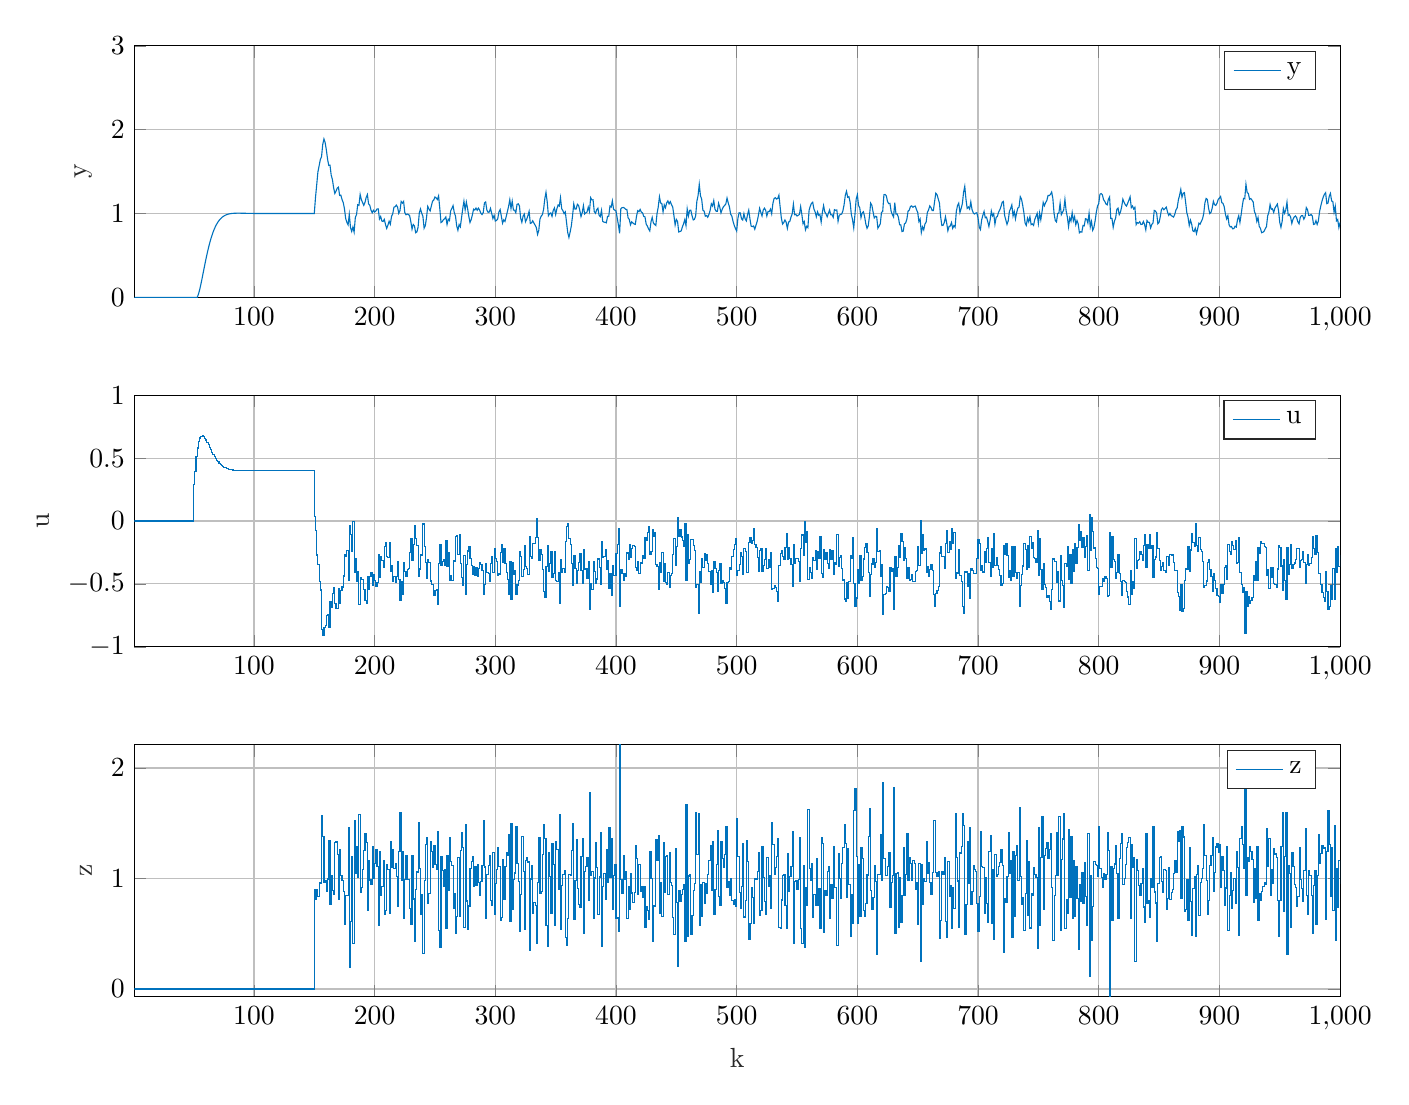
\begin{tikzpicture}

\begin{axis}[%
width=6.028in,
height=1.258in,
at={(1.011in,4.137in)},
scale only axis,
xmin=1,
xmax=1000,
ymin=0,
ymax=3,
ylabel style={font=\color{white!15!black}},
ylabel={y},
axis background/.style={fill=white},
xmajorgrids,
ymajorgrids,
legend style={legend cell align=left, align=left, draw=white!15!black}
]
\addplot [color=mycolor1]
  table[row sep=crcr]{%
1	0\\
2	0\\
3	0\\
4	0\\
5	0\\
6	0\\
7	0\\
8	0\\
9	0\\
10	0\\
11	0\\
12	0\\
13	0\\
14	0\\
15	0\\
16	0\\
17	0\\
18	0\\
19	0\\
20	0\\
21	0\\
22	0\\
23	0\\
24	0\\
25	0\\
26	0\\
27	0\\
28	0\\
29	0\\
30	0\\
31	0\\
32	0\\
33	0\\
34	0\\
35	0\\
36	0\\
37	0\\
38	0\\
39	0\\
40	0\\
41	0\\
42	0\\
43	0\\
44	0\\
45	0\\
46	0\\
47	0\\
48	0\\
49	0\\
50	0\\
51	0\\
52	0\\
53	0\\
54	0.039119\\
55	0.090032\\
56	0.15448\\
57	0.22449\\
58	0.29764\\
59	0.37063\\
60	0.44164\\
61	0.50914\\
62	0.57223\\
63	0.63032\\
64	0.68313\\
65	0.73061\\
66	0.77286\\
67	0.81011\\
68	0.84266\\
69	0.87086\\
70	0.8951\\
71	0.91576\\
72	0.93322\\
73	0.94786\\
74	0.96003\\
75	0.97004\\
76	0.97821\\
77	0.98479\\
78	0.99003\\
79	0.99414\\
80	0.99731\\
81	0.99971\\
82	1.0015\\
83	1.0027\\
84	1.0036\\
85	1.0041\\
86	1.0043\\
87	1.0044\\
88	1.0043\\
89	1.0042\\
90	1.0039\\
91	1.0036\\
92	1.0033\\
93	1.003\\
94	1.0027\\
95	1.0024\\
96	1.0021\\
97	1.0018\\
98	1.0016\\
99	1.0013\\
100	1.0011\\
101	1.001\\
102	1.0008\\
103	1.0007\\
104	1.0005\\
105	1.0004\\
106	1.0003\\
107	1.0003\\
108	1.0002\\
109	1.0002\\
110	1.0001\\
111	1.0001\\
112	1.0001\\
113	1\\
114	1\\
115	1\\
116	1\\
117	0.99999\\
118	0.99998\\
119	0.99998\\
120	0.99998\\
121	0.99998\\
122	0.99998\\
123	0.99998\\
124	0.99998\\
125	0.99998\\
126	0.99998\\
127	0.99998\\
128	0.99998\\
129	0.99998\\
130	0.99998\\
131	0.99998\\
132	0.99999\\
133	0.99999\\
134	0.99999\\
135	0.99999\\
136	0.99999\\
137	0.99999\\
138	0.99999\\
139	0.99999\\
140	0.99999\\
141	0.99999\\
142	0.99999\\
143	0.99999\\
144	0.99999\\
145	0.99999\\
146	0.99999\\
147	0.99999\\
148	0.99999\\
149	0.99999\\
150	0.99999\\
151	1.1911\\
152	1.3423\\
153	1.4966\\
154	1.5691\\
155	1.6432\\
156	1.6774\\
157	1.8242\\
158	1.8897\\
159	1.8448\\
160	1.7591\\
161	1.648\\
162	1.5731\\
163	1.5767\\
164	1.4591\\
165	1.4063\\
166	1.3102\\
167	1.2396\\
168	1.2665\\
169	1.3034\\
170	1.3144\\
171	1.2167\\
172	1.2192\\
173	1.167\\
174	1.1297\\
175	1.0571\\
176	0.94127\\
177	0.89531\\
178	0.86531\\
179	0.99079\\
180	0.83289\\
181	0.78685\\
182	0.84044\\
183	0.77875\\
184	0.95232\\
185	0.98811\\
186	1.1054\\
187	1.0983\\
188	1.2276\\
189	1.1665\\
190	1.1311\\
191	1.0982\\
192	1.1324\\
193	1.1924\\
194	1.2262\\
195	1.114\\
196	1.0984\\
197	1.0412\\
198	1.0087\\
199	1.0389\\
200	1.0178\\
201	1.0306\\
202	1.055\\
203	1.0558\\
204	0.93508\\
205	0.9653\\
206	0.90932\\
207	0.90624\\
208	0.93101\\
209	0.87026\\
210	0.82245\\
211	0.86162\\
212	0.90842\\
213	0.87194\\
214	0.96551\\
215	0.99706\\
216	1.0758\\
217	1.0811\\
218	1.1007\\
219	1.077\\
220	1.0025\\
221	1.0355\\
222	1.1443\\
223	1.125\\
224	1.1447\\
225	1.011\\
226	0.98541\\
227	0.99412\\
228	0.98906\\
229	0.97519\\
230	0.90217\\
231	0.81389\\
232	0.86948\\
233	0.85253\\
234	0.77165\\
235	0.77961\\
236	0.83708\\
237	1.0055\\
238	1.0552\\
239	1.0049\\
240	0.96676\\
241	0.82504\\
242	0.85541\\
243	0.95218\\
244	1.0852\\
245	1.0547\\
246	1.0314\\
247	1.0916\\
248	1.1469\\
249	1.1618\\
250	1.1969\\
251	1.1865\\
252	1.1671\\
253	1.2099\\
254	1.0595\\
255	0.89272\\
256	0.90305\\
257	0.92713\\
258	0.93807\\
259	0.9598\\
260	0.86963\\
261	0.93313\\
262	0.91621\\
263	1.0311\\
264	1.0609\\
265	1.0944\\
266	1.0115\\
267	0.97051\\
268	0.85255\\
269	0.80068\\
270	0.86801\\
271	0.84124\\
272	0.9474\\
273	1.0567\\
274	1.1469\\
275	1.0443\\
276	1.1368\\
277	1.0614\\
278	0.96987\\
279	0.89311\\
280	0.92754\\
281	0.9855\\
282	1.0523\\
283	1.0426\\
284	1.0655\\
285	1.0395\\
286	1.0646\\
287	1.0418\\
288	1.0044\\
289	0.98814\\
290	1.0123\\
291	1.1269\\
292	1.1378\\
293	1.0411\\
294	1.0153\\
295	1.0175\\
296	1.0608\\
297	1.0024\\
298	0.9403\\
299	0.9781\\
300	0.91047\\
301	0.91825\\
302	0.93605\\
303	1.0197\\
304	1.0482\\
305	0.96732\\
306	0.8847\\
307	0.92467\\
308	0.90622\\
309	0.96303\\
310	1.0233\\
311	1.0849\\
312	1.1652\\
313	1.06\\
314	1.1474\\
315	1.0418\\
316	1.0395\\
317	1.0097\\
318	1.11\\
319	1.1157\\
320	1.0902\\
321	0.94516\\
322	0.89568\\
323	0.96774\\
324	0.99377\\
325	0.90233\\
326	0.93264\\
327	0.97357\\
328	1.026\\
329	0.88187\\
330	0.88858\\
331	0.91424\\
332	0.88578\\
333	0.86125\\
334	0.83293\\
335	0.75098\\
336	0.79779\\
337	0.93375\\
338	0.96912\\
339	0.98571\\
340	1.0489\\
341	1.1741\\
342	1.2532\\
343	1.1394\\
344	0.97477\\
345	0.99966\\
346	1.0083\\
347	0.96647\\
348	1.0381\\
349	1.0673\\
350	0.989\\
351	1.0553\\
352	1.1014\\
353	1.0887\\
354	1.1902\\
355	1.058\\
356	1.0339\\
357	0.99873\\
358	1.0204\\
359	0.89679\\
360	0.77534\\
361	0.71486\\
362	0.77926\\
363	0.85344\\
364	0.97214\\
365	1.1154\\
366	1.0528\\
367	1.0544\\
368	1.1104\\
369	1.096\\
370	1.0375\\
371	0.96407\\
372	1.0096\\
373	1.0934\\
374	0.9954\\
375	1.0094\\
376	1.0174\\
377	1.0768\\
378	1.0253\\
379	1.1889\\
380	1.1625\\
381	1.1641\\
382	1.0238\\
383	1.0029\\
384	1.0455\\
385	1.0636\\
386	0.97922\\
387	0.96342\\
388	1.0378\\
389	0.9066\\
390	0.89754\\
391	0.89603\\
392	0.88991\\
393	0.96503\\
394	0.96978\\
395	1.0884\\
396	1.0771\\
397	1.1513\\
398	1.0507\\
399	1.0404\\
400	1.0307\\
401	0.9479\\
402	0.8641\\
403	0.7643\\
404	1.0583\\
405	1.0694\\
406	1.0723\\
407	1.0655\\
408	1.0508\\
409	1.0498\\
410	0.94981\\
411	0.93027\\
412	0.86507\\
413	0.90077\\
414	0.88813\\
415	0.87528\\
416	0.87114\\
417	0.96771\\
418	1.0341\\
419	1.0224\\
420	1.049\\
421	1.0168\\
422	1.0079\\
423	0.96578\\
424	0.96047\\
425	0.87532\\
426	0.84981\\
427	0.81717\\
428	0.79226\\
429	0.90035\\
430	0.95291\\
431	0.88629\\
432	0.87036\\
433	0.85834\\
434	0.99942\\
435	1.0773\\
436	1.2\\
437	1.1261\\
438	1.1183\\
439	1.0201\\
440	1.1035\\
441	1.069\\
442	1.1285\\
443	1.1513\\
444	1.1152\\
445	1.1426\\
446	1.1058\\
447	1.0783\\
448	0.97547\\
449	0.86369\\
450	0.93\\
451	0.90639\\
452	0.77999\\
453	0.78659\\
454	0.79174\\
455	0.841\\
456	0.87727\\
457	0.92756\\
458	0.85624\\
459	1.0551\\
460	0.97118\\
461	1.0382\\
462	1.0404\\
463	0.97453\\
464	0.92421\\
465	0.93138\\
466	0.97104\\
467	1.1456\\
468	1.2143\\
469	1.3483\\
470	1.2121\\
471	1.1711\\
472	1.0402\\
473	1.0304\\
474	0.9691\\
475	0.97668\\
476	0.95591\\
477	0.98832\\
478	1.0373\\
479	1.116\\
480	1.0905\\
481	1.1537\\
482	1.0534\\
483	1.0266\\
484	1.0271\\
485	1.1231\\
486	1.0743\\
487	1.0085\\
488	1.0518\\
489	1.0804\\
490	1.0963\\
491	1.1138\\
492	1.1845\\
493	1.1269\\
494	1.0796\\
495	0.99287\\
496	0.96895\\
497	0.90645\\
498	0.85811\\
499	0.82139\\
500	0.79112\\
501	0.94226\\
502	1.0091\\
503	1.0074\\
504	0.9377\\
505	0.92248\\
506	0.99851\\
507	0.93722\\
508	0.91228\\
509	0.98772\\
510	1.0402\\
511	0.93492\\
512	0.84989\\
513	0.8443\\
514	0.85158\\
515	0.81316\\
516	0.86104\\
517	0.90742\\
518	0.97805\\
519	1.063\\
520	1.0145\\
521	0.97119\\
522	1.041\\
523	1.0641\\
524	1.0404\\
525	0.9704\\
526	1.0243\\
527	1.023\\
528	1.0531\\
529	0.99593\\
530	1.1201\\
531	1.1787\\
532	1.1894\\
533	1.1729\\
534	1.1793\\
535	1.2191\\
536	1.0804\\
537	0.94886\\
538	0.87476\\
539	0.89235\\
540	0.92392\\
541	0.8964\\
542	0.8228\\
543	0.89861\\
544	0.90605\\
545	0.95714\\
546	0.99682\\
547	1.1113\\
548	0.98624\\
549	0.9894\\
550	0.97056\\
551	0.98018\\
552	0.98873\\
553	1.0822\\
554	0.99026\\
555	0.8771\\
556	0.90433\\
557	0.80574\\
558	0.8477\\
559	0.83151\\
560	1.039\\
561	1.0886\\
562	1.1222\\
563	1.1348\\
564	1.0539\\
565	1.0197\\
566	0.96132\\
567	1.0205\\
568	0.97977\\
569	0.98758\\
570	0.89851\\
571	1.0128\\
572	1.095\\
573	1.0205\\
574	0.9965\\
575	0.96077\\
576	1.004\\
577	1.042\\
578	0.98385\\
579	0.98561\\
580	0.95492\\
581	1.0466\\
582	1.0395\\
583	1.0425\\
584	0.90767\\
585	0.97847\\
586	0.98914\\
587	0.99387\\
588	1.0313\\
589	1.105\\
590	1.2159\\
591	1.2658\\
592	1.1933\\
593	1.2014\\
594	1.1343\\
595	0.99099\\
596	0.92645\\
597	0.82908\\
598	0.98883\\
599	1.1707\\
600	1.2242\\
601	1.0946\\
602	1.0686\\
603	0.95156\\
604	1.0084\\
605	1.0223\\
606	0.96488\\
607	0.87601\\
608	0.82466\\
609	0.85344\\
610	0.96507\\
611	1.1241\\
612	1.1001\\
613	1.0213\\
614	0.94789\\
615	0.96667\\
616	0.96365\\
617	0.82606\\
618	0.84971\\
619	0.87701\\
620	1.0144\\
621	1.0242\\
622	1.2242\\
623	1.2281\\
624	1.2109\\
625	1.1431\\
626	1.1181\\
627	1.1215\\
628	1.0253\\
629	0.98656\\
630	0.95884\\
631	1.1292\\
632	0.99481\\
633	0.99563\\
634	0.9545\\
635	0.86674\\
636	0.86489\\
637	0.78492\\
638	0.79065\\
639	0.87732\\
640	0.88663\\
641	0.9303\\
642	1.029\\
643	1.0405\\
644	1.0842\\
645	1.0911\\
646	1.0747\\
647	1.0855\\
648	1.0889\\
649	1.0463\\
650	1.0146\\
651	0.90458\\
652	0.93404\\
653	0.77281\\
654	0.84113\\
655	0.806\\
656	0.87504\\
657	0.89647\\
658	1.0142\\
659	1.0435\\
660	1.0909\\
661	1.0714\\
662	1.0362\\
663	1.0368\\
664	1.143\\
665	1.243\\
666	1.2251\\
667	1.1756\\
668	1.1261\\
669	0.96468\\
670	0.85781\\
671	0.86059\\
672	0.89119\\
673	0.96029\\
674	0.88831\\
675	0.79508\\
676	0.84625\\
677	0.85149\\
678	0.89262\\
679	0.82397\\
680	0.85633\\
681	0.83668\\
682	1.0257\\
683	1.0955\\
684	1.1238\\
685	1.0115\\
686	1.0611\\
687	1.1162\\
688	1.2521\\
689	1.3238\\
690	1.1695\\
691	1.0624\\
692	1.0785\\
693	1.0534\\
694	1.1388\\
695	1.05\\
696	1.0085\\
697	0.99472\\
698	1.0047\\
699	1.0094\\
700	0.94739\\
701	0.83861\\
702	0.80935\\
703	0.92496\\
704	0.98015\\
705	1.0248\\
706	0.94943\\
707	0.95697\\
708	0.90677\\
709	0.84665\\
710	0.91968\\
711	1.0307\\
712	0.97181\\
713	0.99822\\
714	0.87288\\
715	0.95422\\
716	0.96564\\
717	1.0161\\
718	1.0436\\
719	1.0829\\
720	1.1347\\
721	1.1445\\
722	0.97893\\
723	0.92475\\
724	0.87035\\
725	0.91279\\
726	1.0267\\
727	1.0593\\
728	1.1029\\
729	0.97047\\
730	1.0253\\
731	0.9368\\
732	1.0118\\
733	1.0662\\
734	1.0776\\
735	1.202\\
736	1.1733\\
737	1.0989\\
738	1.0087\\
739	0.88549\\
740	0.85829\\
741	0.94501\\
742	0.90224\\
743	0.96284\\
744	0.86765\\
745	0.87643\\
746	0.85833\\
747	0.92858\\
748	0.96625\\
749	1.002\\
750	0.88159\\
751	1.007\\
752	0.92624\\
753	1.0189\\
754	1.1326\\
755	1.0935\\
756	1.1305\\
757	1.1558\\
758	1.2149\\
759	1.2148\\
760	1.2277\\
761	1.2568\\
762	1.1791\\
763	0.99999\\
764	0.91707\\
765	0.90003\\
766	1.0004\\
767	1.0059\\
768	1.1238\\
769	0.98609\\
770	1.0133\\
771	1.0445\\
772	1.1686\\
773	1.0307\\
774	0.95879\\
775	0.84367\\
776	0.94825\\
777	0.9091\\
778	1.012\\
779	0.91301\\
780	0.96222\\
781	0.86724\\
782	0.91675\\
783	0.87484\\
784	0.77009\\
785	0.78253\\
786	0.77892\\
787	0.85794\\
788	0.85339\\
789	0.93863\\
790	0.93434\\
791	0.88779\\
792	1.0036\\
793	0.84107\\
794	0.90524\\
795	0.80049\\
796	0.83259\\
797	0.91252\\
798	1.0141\\
799	1.0896\\
800	1.119\\
801	1.2296\\
802	1.2375\\
803	1.2241\\
804	1.165\\
805	1.1447\\
806	1.1138\\
807	1.1036\\
808	1.1703\\
809	1.198\\
810	0.93927\\
811	0.94036\\
812	0.83582\\
813	0.90829\\
814	0.94624\\
815	1.0493\\
816	1.0639\\
817	0.98709\\
818	1.0177\\
819	1.0789\\
820	1.1706\\
821	1.1341\\
822	1.1048\\
823	1.0889\\
824	1.1233\\
825	1.1602\\
826	1.2002\\
827	1.0698\\
828	1.0895\\
829	1.0538\\
830	1.0749\\
831	0.86762\\
832	0.89196\\
833	0.88547\\
834	0.9027\\
835	0.86908\\
836	0.87169\\
837	0.90535\\
838	0.86955\\
839	0.80582\\
840	0.91653\\
841	0.89484\\
842	0.89526\\
843	0.82894\\
844	0.87101\\
845	0.88836\\
846	1.0368\\
847	1.0296\\
848	1.0059\\
849	0.87767\\
850	0.89442\\
851	0.96241\\
852	1.0503\\
853	1.0653\\
854	1.045\\
855	1.0606\\
856	1.0766\\
857	1.0182\\
858	0.97864\\
859	1.0011\\
860	0.97597\\
861	0.96768\\
862	0.95757\\
863	0.9905\\
864	1.043\\
865	1.0677\\
866	1.1625\\
867	1.2181\\
868	1.2878\\
869	1.1934\\
870	1.2423\\
871	1.2494\\
872	1.1361\\
873	1.0103\\
874	0.95647\\
875	0.85771\\
876	0.92139\\
877	0.87501\\
878	0.79326\\
879	0.78485\\
880	0.82425\\
881	0.76133\\
882	0.81924\\
883	0.88534\\
884	0.87336\\
885	0.90552\\
886	0.93627\\
887	0.99833\\
888	1.1281\\
889	1.1801\\
890	1.1688\\
891	1.0655\\
892	1.0003\\
893	1.0134\\
894	1.0637\\
895	1.1458\\
896	1.1049\\
897	1.0969\\
898	1.1223\\
899	1.1685\\
900	1.1848\\
901	1.2038\\
902	1.1296\\
903	1.1213\\
904	1.079\\
905	0.99166\\
906	0.93631\\
907	0.97523\\
908	0.86646\\
909	0.83976\\
910	0.84526\\
911	0.81742\\
912	0.82191\\
913	0.84852\\
914	0.83902\\
915	0.92722\\
916	0.97346\\
917	0.89351\\
918	0.98651\\
919	1.0937\\
920	1.1809\\
921	1.1761\\
922	1.3493\\
923	1.2507\\
924	1.239\\
925	1.1695\\
926	1.1789\\
927	1.1604\\
928	1.1374\\
929	1.0245\\
930	0.99126\\
931	0.90566\\
932	0.95304\\
933	0.84697\\
934	0.82394\\
935	0.77115\\
936	0.77692\\
937	0.78839\\
938	0.8194\\
939	0.8437\\
940	0.97414\\
941	1.0162\\
942	1.108\\
943	1.0508\\
944	1.0563\\
945	1.0135\\
946	1.0649\\
947	1.0892\\
948	1.1132\\
949	1.0359\\
950	0.89553\\
951	0.83578\\
952	0.90692\\
953	1.0604\\
954	1.0049\\
955	1.0435\\
956	1.1368\\
957	0.97787\\
958	0.98678\\
959	0.95782\\
960	0.8823\\
961	0.93181\\
962	0.95896\\
963	0.97132\\
964	0.95134\\
965	0.90088\\
966	0.87743\\
967	0.95483\\
968	0.97454\\
969	0.9761\\
970	0.93271\\
971	0.9626\\
972	1.0708\\
973	1.0461\\
974	0.97821\\
975	0.97895\\
976	0.98926\\
977	0.96991\\
978	0.87012\\
979	0.87527\\
980	0.9156\\
981	0.87011\\
982	0.91213\\
983	1.0243\\
984	1.0896\\
985	1.1485\\
986	1.195\\
987	1.229\\
988	1.2482\\
989	1.1178\\
990	1.1257\\
991	1.2052\\
992	1.2404\\
993	1.1497\\
994	1.1427\\
995	1.0163\\
996	1.0871\\
997	0.91246\\
998	0.92898\\
999	0.83376\\
1000	0.89373\\
};
\addlegendentry{y}

\end{axis}

\begin{axis}[%
width=6.028in,
height=1.258in,
at={(1.011in,2.39in)},
scale only axis,
xmin=1,
xmax=1000,
ymin=-1,
ymax=1,
ylabel style={font=\color{white!15!black}},
ylabel={u},
axis background/.style={fill=white},
xmajorgrids,
ymajorgrids,
legend style={legend cell align=left, align=left, draw=white!15!black}
]
\addplot[const plot, color=mycolor1] table[row sep=crcr] {%
1	0\\
2	0\\
3	0\\
4	0\\
5	0\\
6	0\\
7	0\\
8	0\\
9	0\\
10	0\\
11	0\\
12	0\\
13	0\\
14	0\\
15	0\\
16	0\\
17	0\\
18	0\\
19	0\\
20	0\\
21	0\\
22	0\\
23	0\\
24	0\\
25	0\\
26	0\\
27	0\\
28	0\\
29	0\\
30	0\\
31	0\\
32	0\\
33	0\\
34	0\\
35	0\\
36	0\\
37	0\\
38	0\\
39	0\\
40	0\\
41	0\\
42	0\\
43	0\\
44	0\\
45	0\\
46	0\\
47	0\\
48	0\\
49	0\\
50	0.28956\\
51	0.39251\\
52	0.5131\\
53	0.58007\\
54	0.63135\\
55	0.65951\\
56	0.67407\\
57	0.67664\\
58	0.67103\\
59	0.65931\\
60	0.64358\\
61	0.62529\\
62	0.60567\\
63	0.58562\\
64	0.56581\\
65	0.54674\\
66	0.52873\\
67	0.512\\
68	0.49669\\
69	0.48283\\
70	0.47042\\
71	0.45942\\
72	0.44977\\
73	0.44136\\
74	0.4341\\
75	0.42788\\
76	0.4226\\
77	0.41815\\
78	0.41444\\
79	0.41136\\
80	0.40884\\
81	0.4068\\
82	0.40516\\
83	0.40387\\
84	0.40286\\
85	0.40209\\
86	0.40151\\
87	0.4011\\
88	0.40081\\
89	0.40063\\
90	0.40052\\
91	0.40048\\
92	0.40048\\
93	0.40051\\
94	0.40057\\
95	0.40065\\
96	0.40073\\
97	0.40082\\
98	0.40091\\
99	0.401\\
100	0.40108\\
101	0.40116\\
102	0.40123\\
103	0.4013\\
104	0.40136\\
105	0.40142\\
106	0.40146\\
107	0.4015\\
108	0.40154\\
109	0.40157\\
110	0.4016\\
111	0.40162\\
112	0.40164\\
113	0.40166\\
114	0.40167\\
115	0.40168\\
116	0.40169\\
117	0.4017\\
118	0.4017\\
119	0.40171\\
120	0.40171\\
121	0.40171\\
122	0.40171\\
123	0.40172\\
124	0.40172\\
125	0.40172\\
126	0.40172\\
127	0.40172\\
128	0.40172\\
129	0.40172\\
130	0.40172\\
131	0.40172\\
132	0.40172\\
133	0.40171\\
134	0.40171\\
135	0.40171\\
136	0.40171\\
137	0.40171\\
138	0.40171\\
139	0.40171\\
140	0.40171\\
141	0.40171\\
142	0.40171\\
143	0.40171\\
144	0.40171\\
145	0.40171\\
146	0.40171\\
147	0.40171\\
148	0.40171\\
149	0.40171\\
150	0.034135\\
151	-0.07511\\
152	-0.27025\\
153	-0.34681\\
154	-0.48319\\
155	-0.54817\\
156	-0.85952\\
157	-0.91219\\
158	-0.84823\\
159	-0.82875\\
160	-0.7489\\
161	-0.7436\\
162	-0.84906\\
163	-0.63914\\
164	-0.68898\\
165	-0.57674\\
166	-0.52697\\
167	-0.65908\\
168	-0.69483\\
169	-0.6972\\
170	-0.53643\\
171	-0.65551\\
172	-0.55003\\
173	-0.52468\\
174	-0.43666\\
175	-0.27052\\
176	-0.28216\\
177	-0.23553\\
178	-0.47337\\
179	-0.037971\\
180	-0.10998\\
181	-0.24399\\
182	-0.002674\\
183	-0.40573\\
184	-0.29506\\
185	-0.48128\\
186	-0.40492\\
187	-0.66628\\
188	-0.45268\\
189	-0.46727\\
190	-0.46821\\
191	-0.5433\\
192	-0.63402\\
193	-0.65616\\
194	-0.43777\\
195	-0.54294\\
196	-0.43948\\
197	-0.41345\\
198	-0.51093\\
199	-0.42417\\
200	-0.47453\\
201	-0.51682\\
202	-0.48794\\
203	-0.26859\\
204	-0.44812\\
205	-0.28499\\
206	-0.31235\\
207	-0.36955\\
208	-0.20156\\
209	-0.17147\\
210	-0.27861\\
211	-0.29344\\
212	-0.17466\\
213	-0.40065\\
214	-0.35726\\
215	-0.47815\\
216	-0.44332\\
217	-0.48466\\
218	-0.44076\\
219	-0.32487\\
220	-0.46638\\
221	-0.62884\\
222	-0.48509\\
223	-0.5842\\
224	-0.32798\\
225	-0.40186\\
226	-0.43671\\
227	-0.38624\\
228	-0.37718\\
229	-0.2499\\
230	-0.13959\\
231	-0.31232\\
232	-0.18759\\
233	-0.038044\\
234	-0.13601\\
235	-0.19463\\
236	-0.43691\\
237	-0.38176\\
238	-0.26727\\
239	-0.2766\\
240	-0.023881\\
241	-0.19955\\
242	-0.32698\\
243	-0.46004\\
244	-0.30845\\
245	-0.32786\\
246	-0.47691\\
247	-0.50804\\
248	-0.50514\\
249	-0.59228\\
250	-0.55328\\
251	-0.54505\\
252	-0.66658\\
253	-0.3405\\
254	-0.18394\\
255	-0.35636\\
256	-0.32524\\
257	-0.30797\\
258	-0.35681\\
259	-0.1526\\
260	-0.35915\\
261	-0.24837\\
262	-0.46847\\
263	-0.43231\\
264	-0.47229\\
265	-0.31411\\
266	-0.31816\\
267	-0.12382\\
268	-0.11161\\
269	-0.26576\\
270	-0.1086\\
271	-0.34093\\
272	-0.45022\\
273	-0.51309\\
274	-0.27695\\
275	-0.58296\\
276	-0.34312\\
277	-0.23811\\
278	-0.20623\\
279	-0.30006\\
280	-0.35415\\
281	-0.42601\\
282	-0.36107\\
283	-0.43164\\
284	-0.36769\\
285	-0.4411\\
286	-0.3809\\
287	-0.33139\\
288	-0.34393\\
289	-0.39315\\
290	-0.58354\\
291	-0.50218\\
292	-0.3362\\
293	-0.40803\\
294	-0.41374\\
295	-0.4773\\
296	-0.33548\\
297	-0.28108\\
298	-0.41025\\
299	-0.21517\\
300	-0.2954\\
301	-0.31926\\
302	-0.43624\\
303	-0.42105\\
304	-0.25286\\
305	-0.18965\\
306	-0.32708\\
307	-0.21682\\
308	-0.341\\
309	-0.40809\\
310	-0.46152\\
311	-0.58258\\
312	-0.32375\\
313	-0.62009\\
314	-0.33398\\
315	-0.4258\\
316	-0.39285\\
317	-0.58229\\
318	-0.50882\\
319	-0.47171\\
320	-0.2455\\
321	-0.27977\\
322	-0.43764\\
323	-0.38222\\
324	-0.19714\\
325	-0.36018\\
326	-0.38068\\
327	-0.42473\\
328	-0.12147\\
329	-0.2796\\
330	-0.29687\\
331	-0.17973\\
332	-0.17875\\
333	-0.13366\\
334	0.022525\\
335	-0.13147\\
336	-0.31407\\
337	-0.23078\\
338	-0.26302\\
339	-0.38744\\
340	-0.55864\\
341	-0.61064\\
342	-0.36017\\
343	-0.19712\\
344	-0.39751\\
345	-0.33915\\
346	-0.24307\\
347	-0.44539\\
348	-0.41491\\
349	-0.24149\\
350	-0.47456\\
351	-0.48081\\
352	-0.40967\\
353	-0.65774\\
354	-0.30736\\
355	-0.40831\\
356	-0.37434\\
357	-0.40841\\
358	-0.16145\\
359	-0.04402\\
360	-0.021011\\
361	-0.14247\\
362	-0.18696\\
363	-0.33765\\
364	-0.51281\\
365	-0.27385\\
366	-0.38056\\
367	-0.49642\\
368	-0.39341\\
369	-0.32668\\
370	-0.25552\\
371	-0.39492\\
372	-0.49496\\
373	-0.2284\\
374	-0.38269\\
375	-0.37722\\
376	-0.45811\\
377	-0.32556\\
378	-0.69981\\
379	-0.49586\\
380	-0.54702\\
381	-0.3234\\
382	-0.40097\\
383	-0.49277\\
384	-0.46078\\
385	-0.30226\\
386	-0.36631\\
387	-0.50498\\
388	-0.16149\\
389	-0.29133\\
390	-0.28295\\
391	-0.22665\\
392	-0.38842\\
393	-0.31345\\
394	-0.53998\\
395	-0.42119\\
396	-0.58804\\
397	-0.35223\\
398	-0.43389\\
399	-0.43325\\
400	-0.25789\\
401	-0.18894\\
402	-0.058704\\
403	-0.67907\\
404	-0.38558\\
405	-0.41628\\
406	-0.47105\\
407	-0.41376\\
408	-0.43891\\
409	-0.25399\\
410	-0.30819\\
411	-0.18662\\
412	-0.2903\\
413	-0.22145\\
414	-0.19338\\
415	-0.20019\\
416	-0.37001\\
417	-0.3947\\
418	-0.3223\\
419	-0.41385\\
420	-0.32627\\
421	-0.34007\\
422	-0.27499\\
423	-0.2939\\
424	-0.12986\\
425	-0.15148\\
426	-0.094592\\
427	-0.046436\\
428	-0.26531\\
429	-0.23892\\
430	-0.066066\\
431	-0.12607\\
432	-0.093722\\
433	-0.34882\\
434	-0.36234\\
435	-0.54128\\
436	-0.3264\\
437	-0.41134\\
438	-0.24675\\
439	-0.48378\\
440	-0.33844\\
441	-0.48762\\
442	-0.50175\\
443	-0.40964\\
444	-0.52876\\
445	-0.43328\\
446	-0.42026\\
447	-0.26422\\
448	-0.13635\\
449	-0.3533\\
450	-0.20262\\
451	0.023767\\
452	-0.12207\\
453	-0.071357\\
454	-0.12683\\
455	-0.15393\\
456	-0.2038\\
457	-0.021958\\
458	-0.47635\\
459	-0.10996\\
460	-0.33356\\
461	-0.30887\\
462	-0.14828\\
463	-0.1475\\
464	-0.19124\\
465	-0.23288\\
466	-0.53041\\
467	-0.50505\\
468	-0.73728\\
469	-0.40299\\
470	-0.49089\\
471	-0.29746\\
472	-0.37207\\
473	-0.26225\\
474	-0.31435\\
475	-0.26647\\
476	-0.33483\\
477	-0.39867\\
478	-0.50095\\
479	-0.39444\\
480	-0.56477\\
481	-0.3235\\
482	-0.37481\\
483	-0.40931\\
484	-0.56371\\
485	-0.3902\\
486	-0.33488\\
487	-0.49309\\
488	-0.47719\\
489	-0.48826\\
490	-0.53321\\
491	-0.65652\\
492	-0.49069\\
493	-0.48191\\
494	-0.37187\\
495	-0.38772\\
496	-0.27876\\
497	-0.22786\\
498	-0.19006\\
499	-0.13737\\
500	-0.4348\\
501	-0.39668\\
502	-0.34304\\
503	-0.25153\\
504	-0.27929\\
505	-0.42101\\
506	-0.21519\\
507	-0.24123\\
508	-0.41011\\
509	-0.40634\\
510	-0.17112\\
511	-0.13467\\
512	-0.18117\\
513	-0.15416\\
514	-0.062363\\
515	-0.1866\\
516	-0.2077\\
517	-0.2882\\
518	-0.3992\\
519	-0.2342\\
520	-0.22244\\
521	-0.40212\\
522	-0.35398\\
523	-0.30245\\
524	-0.21689\\
525	-0.37878\\
526	-0.30884\\
527	-0.37063\\
528	-0.25132\\
529	-0.54292\\
530	-0.53653\\
531	-0.51557\\
532	-0.52667\\
533	-0.56375\\
534	-0.64272\\
535	-0.35356\\
536	-0.25728\\
537	-0.23195\\
538	-0.2823\\
539	-0.30163\\
540	-0.21179\\
541	-0.1001\\
542	-0.30458\\
543	-0.21342\\
544	-0.29877\\
545	-0.34305\\
546	-0.51676\\
547	-0.18371\\
548	-0.33648\\
549	-0.29462\\
550	-0.29462\\
551	-0.31893\\
552	-0.48339\\
553	-0.21916\\
554	-0.11115\\
555	-0.27284\\
556	-0.0024715\\
557	-0.16842\\
558	-0.086786\\
559	-0.46635\\
560	-0.37167\\
561	-0.41155\\
562	-0.45722\\
563	-0.28748\\
564	-0.31682\\
565	-0.23326\\
566	-0.38151\\
567	-0.24198\\
568	-0.29691\\
569	-0.12702\\
570	-0.415\\
571	-0.45214\\
572	-0.23039\\
573	-0.30601\\
574	-0.2487\\
575	-0.33956\\
576	-0.37539\\
577	-0.2267\\
578	-0.30414\\
579	-0.23547\\
580	-0.42483\\
581	-0.32671\\
582	-0.34784\\
583	-0.10752\\
584	-0.36199\\
585	-0.29281\\
586	-0.27626\\
587	-0.37442\\
588	-0.46875\\
589	-0.61975\\
590	-0.63892\\
591	-0.49169\\
592	-0.61614\\
593	-0.48183\\
594	-0.27092\\
595	-0.29771\\
596	-0.13365\\
597	-0.49956\\
598	-0.67656\\
599	-0.61161\\
600	-0.38949\\
601	-0.49687\\
602	-0.27434\\
603	-0.4751\\
604	-0.44163\\
605	-0.30192\\
606	-0.21294\\
607	-0.17972\\
608	-0.24813\\
609	-0.40858\\
610	-0.59989\\
611	-0.42341\\
612	-0.34181\\
613	-0.29514\\
614	-0.37013\\
615	-0.32747\\
616	-0.062882\\
617	-0.24423\\
618	-0.23557\\
619	-0.44094\\
620	-0.34735\\
621	-0.73958\\
622	-0.58113\\
623	-0.5773\\
624	-0.52177\\
625	-0.52804\\
626	-0.56187\\
627	-0.37314\\
628	-0.40075\\
629	-0.37477\\
630	-0.7022\\
631	-0.28057\\
632	-0.44051\\
633	-0.37297\\
634	-0.19442\\
635	-0.28866\\
636	-0.10355\\
637	-0.16365\\
638	-0.30988\\
639	-0.21045\\
640	-0.29889\\
641	-0.45372\\
642	-0.37103\\
643	-0.47207\\
644	-0.46251\\
645	-0.42646\\
646	-0.48272\\
647	-0.47972\\
648	-0.39926\\
649	-0.39234\\
650	-0.20659\\
651	-0.35632\\
652	0.0041204\\
653	-0.26148\\
654	-0.10696\\
655	-0.23263\\
656	-0.22228\\
657	-0.40888\\
658	-0.3646\\
659	-0.44335\\
660	-0.38759\\
661	-0.34459\\
662	-0.39095\\
663	-0.58567\\
664	-0.67705\\
665	-0.57922\\
666	-0.55224\\
667	-0.52312\\
668	-0.25406\\
669	-0.20291\\
670	-0.28071\\
671	-0.28408\\
672	-0.37756\\
673	-0.17793\\
674	-0.072529\\
675	-0.24975\\
676	-0.16079\\
677	-0.22462\\
678	-0.06298\\
679	-0.1765\\
680	-0.093492\\
681	-0.45322\\
682	-0.40795\\
683	-0.41574\\
684	-0.22814\\
685	-0.43295\\
686	-0.47855\\
687	-0.68131\\
688	-0.73109\\
689	-0.40533\\
690	-0.39987\\
691	-0.52347\\
692	-0.41543\\
693	-0.61719\\
694	-0.37714\\
695	-0.39048\\
696	-0.41566\\
697	-0.41405\\
698	-0.41671\\
699	-0.29615\\
700	-0.14598\\
701	-0.17987\\
702	-0.38975\\
703	-0.3548\\
704	-0.40563\\
705	-0.24465\\
706	-0.33163\\
707	-0.21913\\
708	-0.13237\\
709	-0.32768\\
710	-0.43909\\
711	-0.21879\\
712	-0.36538\\
713	-0.096035\\
714	-0.3518\\
715	-0.28804\\
716	-0.35344\\
717	-0.38868\\
718	-0.43543\\
719	-0.51332\\
720	-0.49728\\
721	-0.19143\\
722	-0.26364\\
723	-0.18178\\
724	-0.27168\\
725	-0.44596\\
726	-0.39047\\
727	-0.47243\\
728	-0.20087\\
729	-0.43738\\
730	-0.203\\
731	-0.41267\\
732	-0.45739\\
733	-0.41139\\
734	-0.67792\\
735	-0.51229\\
736	-0.4242\\
737	-0.35717\\
738	-0.18054\\
739	-0.22708\\
740	-0.38786\\
741	-0.19205\\
742	-0.36546\\
743	-0.12592\\
744	-0.21669\\
745	-0.17088\\
746	-0.28823\\
747	-0.2947\\
748	-0.32644\\
749	-0.076824\\
750	-0.43655\\
751	-0.13923\\
752	-0.38825\\
753	-0.54256\\
754	-0.33809\\
755	-0.50385\\
756	-0.52925\\
757	-0.61107\\
758	-0.59074\\
759	-0.63929\\
760	-0.70648\\
761	-0.54417\\
762	-0.30154\\
763	-0.31917\\
764	-0.32086\\
765	-0.49014\\
766	-0.40085\\
767	-0.63603\\
768	-0.27617\\
769	-0.47308\\
770	-0.51066\\
771	-0.68394\\
772	-0.33472\\
773	-0.35743\\
774	-0.20246\\
775	-0.46106\\
776	-0.26675\\
777	-0.49703\\
778	-0.22455\\
779	-0.40463\\
780	-0.1809\\
781	-0.33919\\
782	-0.21115\\
783	-0.024891\\
784	-0.15325\\
785	-0.08657\\
786	-0.21221\\
787	-0.12828\\
788	-0.28902\\
789	-0.20281\\
790	-0.11539\\
791	-0.39553\\
792	0.053045\\
793	-0.23613\\
794	0.031456\\
795	-0.083163\\
796	-0.21476\\
797	-0.29513\\
798	-0.3666\\
799	-0.37902\\
800	-0.58767\\
801	-0.51761\\
802	-0.51811\\
803	-0.45707\\
804	-0.47814\\
805	-0.44317\\
806	-0.45465\\
807	-0.59931\\
808	-0.59109\\
809	-0.090693\\
810	-0.37074\\
811	-0.12198\\
812	-0.30636\\
813	-0.31985\\
814	-0.45483\\
815	-0.40906\\
816	-0.26352\\
817	-0.41518\\
818	-0.48426\\
819	-0.5946\\
820	-0.46988\\
821	-0.47763\\
822	-0.48904\\
823	-0.55899\\
824	-0.6044\\
825	-0.66089\\
826	-0.39552\\
827	-0.58041\\
828	-0.48327\\
829	-0.53914\\
830	-0.14186\\
831	-0.38007\\
832	-0.31104\\
833	-0.30472\\
834	-0.24493\\
835	-0.26502\\
836	-0.31311\\
837	-0.19717\\
838	-0.10964\\
839	-0.37268\\
840	-0.18991\\
841	-0.21529\\
842	-0.10452\\
843	-0.218\\
844	-0.19586\\
845	-0.45067\\
846	-0.30408\\
847	-0.2861\\
848	-0.089634\\
849	-0.22192\\
850	-0.31094\\
851	-0.39161\\
852	-0.36153\\
853	-0.33144\\
854	-0.39474\\
855	-0.40703\\
856	-0.28429\\
857	-0.27902\\
858	-0.35283\\
859	-0.26352\\
860	-0.27683\\
861	-0.26721\\
862	-0.32629\\
863	-0.39458\\
864	-0.39499\\
865	-0.57093\\
866	-0.60207\\
867	-0.70785\\
868	-0.50184\\
869	-0.71665\\
870	-0.69401\\
871	-0.47153\\
872	-0.38145\\
873	-0.38354\\
874	-0.20466\\
875	-0.4043\\
876	-0.23041\\
877	-0.10196\\
878	-0.16988\\
879	-0.2046\\
880	-0.019367\\
881	-0.19227\\
882	-0.2396\\
883	-0.13008\\
884	-0.2257\\
885	-0.24498\\
886	-0.32186\\
887	-0.52461\\
888	-0.51117\\
889	-0.47644\\
890	-0.32894\\
891	-0.30766\\
892	-0.38209\\
893	-0.44312\\
894	-0.55717\\
895	-0.42012\\
896	-0.4708\\
897	-0.53925\\
898	-0.59382\\
899	-0.60167\\
900	-0.64724\\
901	-0.50611\\
902	-0.57782\\
903	-0.50682\\
904	-0.3711\\
905	-0.35635\\
906	-0.46103\\
907	-0.1891\\
908	-0.24525\\
909	-0.26524\\
910	-0.16109\\
911	-0.19601\\
912	-0.22582\\
913	-0.15895\\
914	-0.3359\\
915	-0.33023\\
916	-0.13325\\
917	-0.41226\\
918	-0.50711\\
919	-0.56693\\
920	-0.5294\\
921	-0.89766\\
922	-0.56058\\
923	-0.67842\\
924	-0.59725\\
925	-0.65662\\
926	-0.63267\\
927	-0.60951\\
928	-0.42991\\
929	-0.47567\\
930	-0.32511\\
931	-0.4737\\
932	-0.2122\\
933	-0.25531\\
934	-0.16569\\
935	-0.18104\\
936	-0.18197\\
937	-0.20499\\
938	-0.21153\\
939	-0.43044\\
940	-0.38212\\
941	-0.53651\\
942	-0.36907\\
943	-0.44682\\
944	-0.37186\\
945	-0.49736\\
946	-0.50151\\
947	-0.52831\\
948	-0.38109\\
949	-0.19445\\
950	-0.207\\
951	-0.35727\\
952	-0.54844\\
953	-0.30405\\
954	-0.47247\\
955	-0.62342\\
956	-0.21036\\
957	-0.42393\\
958	-0.34656\\
959	-0.18538\\
960	-0.37433\\
961	-0.3477\\
962	-0.33347\\
963	-0.30611\\
964	-0.22143\\
965	-0.21711\\
966	-0.37137\\
967	-0.31563\\
968	-0.30937\\
969	-0.24108\\
970	-0.3301\\
971	-0.49952\\
972	-0.34449\\
973	-0.26896\\
974	-0.35009\\
975	-0.3394\\
976	-0.28688\\
977	-0.12375\\
978	-0.22091\\
979	-0.26464\\
980	-0.11546\\
981	-0.25217\\
982	-0.41439\\
983	-0.4179\\
984	-0.50424\\
985	-0.56756\\
986	-0.60629\\
987	-0.64095\\
988	-0.39873\\
989	-0.56171\\
990	-0.69925\\
991	-0.67705\\
992	-0.51629\\
993	-0.62143\\
994	-0.37744\\
995	-0.62671\\
996	-0.21906\\
997	-0.40619\\
998	-0.20383\\
999	-0.36051\\
1000	-0.27265\\
};
\addlegendentry{u}

\end{axis}

\begin{axis}[%
width=6.028in,
height=1.258in,
at={(1.011in,0.642in)},
scale only axis,
xmin=1,
xmax=1000,
xlabel style={font=\color{white!15!black}},
xlabel={k},
ymin=-0.066865,
ymax=2.2099,
ylabel style={font=\color{white!15!black}},
ylabel={z},
axis background/.style={fill=white},
xmajorgrids,
ymajorgrids,
legend style={legend cell align=left, align=left, draw=white!15!black}
]
\addplot[const plot, color=mycolor1] table[row sep=crcr] {%
1	0\\
2	0\\
3	0\\
4	0\\
5	0\\
6	0\\
7	0\\
8	0\\
9	0\\
10	0\\
11	0\\
12	0\\
13	0\\
14	0\\
15	0\\
16	0\\
17	0\\
18	0\\
19	0\\
20	0\\
21	0\\
22	0\\
23	0\\
24	0\\
25	0\\
26	0\\
27	0\\
28	0\\
29	0\\
30	0\\
31	0\\
32	0\\
33	0\\
34	0\\
35	0\\
36	0\\
37	0\\
38	0\\
39	0\\
40	0\\
41	0\\
42	0\\
43	0\\
44	0\\
45	0\\
46	0\\
47	0\\
48	0\\
49	0\\
50	0\\
51	0\\
52	0\\
53	0\\
54	0\\
55	0\\
56	0\\
57	0\\
58	0\\
59	0\\
60	0\\
61	0\\
62	0\\
63	0\\
64	0\\
65	0\\
66	0\\
67	0\\
68	0\\
69	0\\
70	0\\
71	0\\
72	0\\
73	0\\
74	0\\
75	0\\
76	0\\
77	0\\
78	0\\
79	0\\
80	0\\
81	0\\
82	0\\
83	0\\
84	0\\
85	0\\
86	0\\
87	0\\
88	0\\
89	0\\
90	0\\
91	0\\
92	0\\
93	0\\
94	0\\
95	0\\
96	0\\
97	0\\
98	0\\
99	0\\
100	0\\
101	0\\
102	0\\
103	0\\
104	0\\
105	0\\
106	0\\
107	0\\
108	0\\
109	0\\
110	0\\
111	0\\
112	0\\
113	0\\
114	0\\
115	0\\
116	0\\
117	0\\
118	0\\
119	0\\
120	0\\
121	0\\
122	0\\
123	0\\
124	0\\
125	0\\
126	0\\
127	0\\
128	0\\
129	0\\
130	0\\
131	0\\
132	0\\
133	0\\
134	0\\
135	0\\
136	0\\
137	0\\
138	0\\
139	0\\
140	0\\
141	0\\
142	0\\
143	0\\
144	0\\
145	0\\
146	0\\
147	0\\
148	0\\
149	0\\
150	0.8962\\
151	0.80968\\
152	0.90378\\
153	0.83425\\
154	0.96277\\
155	0.955\\
156	1.5726\\
157	1.3801\\
158	0.96658\\
159	0.97771\\
160	0.88619\\
161	0.99606\\
162	1.3471\\
163	0.7619\\
164	1.0277\\
165	0.88895\\
166	0.85326\\
167	1.3241\\
168	1.3332\\
169	1.2141\\
170	0.80616\\
171	1.2629\\
172	1.0256\\
173	0.98181\\
174	0.88149\\
175	0.58608\\
176	0.84508\\
177	0.84679\\
178	1.4581\\
179	0.19958\\
180	0.60897\\
181	1.1986\\
182	0.41525\\
183	1.5202\\
184	1.0423\\
185	1.2875\\
186	1.0099\\
187	1.58\\
188	0.8723\\
189	0.91935\\
190	1.0811\\
191	1.2562\\
192	1.4087\\
193	1.323\\
194	0.70733\\
195	1.166\\
196	0.98674\\
197	0.94422\\
198	1.2895\\
199	1.0046\\
200	1.1369\\
201	1.2603\\
202	1.1112\\
203	0.57411\\
204	1.2474\\
205	0.84448\\
206	0.92646\\
207	1.1634\\
208	0.67318\\
209	0.71428\\
210	1.1295\\
211	1.0781\\
212	0.68564\\
213	1.336\\
214	1.1\\
215	1.2594\\
216	1.0929\\
217	1.1363\\
218	1.0203\\
219	0.75159\\
220	1.2451\\
221	1.5949\\
222	0.97969\\
223	1.2402\\
224	0.63748\\
225	0.99193\\
226	1.2053\\
227	0.98977\\
228	0.98947\\
229	0.72673\\
230	0.58579\\
231	1.2074\\
232	0.81476\\
233	0.43042\\
234	0.90438\\
235	1.0591\\
236	1.5079\\
237	1.0894\\
238	0.67602\\
239	0.85465\\
240	0.31779\\
241	0.97935\\
242	1.3099\\
243	1.3687\\
244	0.77166\\
245	0.86544\\
246	1.3302\\
247	1.2483\\
248	1.0997\\
249	1.2974\\
250	1.1275\\
251	1.0853\\
252	1.4277\\
253	0.52896\\
254	0.37475\\
255	1.201\\
256	1.0749\\
257	0.92477\\
258	1.0827\\
259	0.54875\\
260	1.209\\
261	0.89369\\
262	1.3731\\
263	1.1571\\
264	1.1196\\
265	0.7271\\
266	0.86142\\
267	0.50677\\
268	0.6584\\
269	1.1905\\
270	0.65978\\
271	1.2524\\
272	1.4119\\
273	1.2773\\
274	0.56006\\
275	1.4905\\
276	0.79671\\
277	0.53821\\
278	0.751\\
279	1.0891\\
280	1.1508\\
281	1.1984\\
282	0.92913\\
283	1.1103\\
284	0.93891\\
285	1.1269\\
286	0.96112\\
287	0.84365\\
288	0.97043\\
289	1.1166\\
290	1.5231\\
291	1.1045\\
292	0.63599\\
293	1.04\\
294	1.1147\\
295	1.2084\\
296	0.79837\\
297	0.75525\\
298	1.2327\\
299	0.67211\\
300	0.95396\\
301	1.0833\\
302	1.2792\\
303	1.1093\\
304	0.62418\\
305	0.64581\\
306	1.1703\\
307	0.81291\\
308	1.1118\\
309	1.2385\\
310	1.2061\\
311	1.3995\\
312	0.61458\\
313	1.4987\\
314	0.71997\\
315	0.99369\\
316	1.05\\
317	1.4725\\
318	1.138\\
319	0.9757\\
320	0.52241\\
321	0.85512\\
322	1.3799\\
323	1.0615\\
324	0.54026\\
325	1.159\\
326	1.1915\\
327	1.1494\\
328	0.3517\\
329	0.99542\\
330	1.1159\\
331	0.68519\\
332	0.7793\\
333	0.75641\\
334	0.41338\\
335	0.96687\\
336	1.3748\\
337	0.8681\\
338	0.88331\\
339	1.2197\\
340	1.4914\\
341	1.3594\\
342	0.57378\\
343	0.38736\\
344	1.232\\
345	1.0212\\
346	0.687\\
347	1.3192\\
348	1.1233\\
349	0.5742\\
350	1.3364\\
351	1.2615\\
352	0.90295\\
353	1.5766\\
354	0.54285\\
355	0.94067\\
356	1.0358\\
357	1.0729\\
358	0.46507\\
359	0.39023\\
360	0.63416\\
361	1.033\\
362	1.0307\\
363	1.2525\\
364	1.4951\\
365	0.62674\\
366	0.98599\\
367	1.3539\\
368	0.90966\\
369	0.76109\\
370	0.73581\\
371	1.1966\\
372	1.3599\\
373	0.50613\\
374	1.0653\\
375	1.1105\\
376	1.1925\\
377	0.79751\\
378	1.7777\\
379	1.0252\\
380	1.063\\
381	0.63512\\
382	1.0049\\
383	1.3287\\
384	1.1016\\
385	0.67716\\
386	1.0135\\
387	1.4119\\
388	0.38952\\
389	0.93052\\
390	1.0484\\
391	0.81277\\
392	1.2644\\
393	0.96541\\
394	1.4628\\
395	1.0133\\
396	1.3619\\
397	0.72299\\
398	1.0247\\
399	1.1302\\
400	0.64045\\
401	0.64292\\
402	0.52526\\
403	2.2099\\
404	0.98977\\
405	0.86791\\
406	1.2052\\
407	0.9904\\
408	1.0671\\
409	0.63877\\
410	0.93068\\
411	0.72349\\
412	1.0473\\
413	0.8689\\
414	0.7817\\
415	0.87458\\
416	1.2984\\
417	1.1849\\
418	0.85186\\
419	1.1276\\
420	0.8831\\
421	0.93143\\
422	0.82838\\
423	0.92604\\
424	0.55695\\
425	0.75053\\
426	0.71308\\
427	0.6266\\
428	1.2432\\
429	0.99729\\
430	0.42739\\
431	0.75917\\
432	0.75153\\
433	1.3518\\
434	1.1593\\
435	1.3848\\
436	0.68291\\
437	0.96563\\
438	0.65494\\
439	1.3286\\
440	0.87529\\
441	1.1984\\
442	1.2061\\
443	0.85691\\
444	1.2318\\
445	0.96067\\
446	0.93375\\
447	0.64471\\
448	0.49561\\
449	1.2672\\
450	0.78439\\
451	0.20586\\
452	0.89291\\
453	0.79489\\
454	0.85623\\
455	0.90074\\
456	0.94662\\
457	0.42967\\
458	1.6706\\
459	0.47607\\
460	1.0223\\
461	1.0322\\
462	0.49059\\
463	0.66466\\
464	0.89503\\
465	0.95117\\
466	1.5999\\
467	1.2192\\
468	1.5854\\
469	0.57714\\
470	0.94638\\
471	0.65886\\
472	0.96355\\
473	0.77615\\
474	0.95123\\
475	0.86884\\
476	1.0398\\
477	1.1656\\
478	1.3001\\
479	0.89482\\
480	1.3383\\
481	0.6732\\
482	0.90376\\
483	1.1285\\
484	1.4321\\
485	0.83562\\
486	0.75308\\
487	1.3301\\
488	1.1819\\
489	1.1036\\
490	1.2191\\
491	1.4719\\
492	0.91921\\
493	0.96937\\
494	0.84376\\
495	0.99734\\
496	0.80152\\
497	0.76812\\
498	0.8057\\
499	0.74681\\
500	1.5445\\
501	1.1983\\
502	0.87137\\
503	0.73117\\
504	0.9282\\
505	1.315\\
506	0.65205\\
507	0.80346\\
508	1.3477\\
509	1.1515\\
510	0.45048\\
511	0.59278\\
512	0.92044\\
513	0.83078\\
514	0.59042\\
515	0.99657\\
516	0.992\\
517	1.0656\\
518	1.2394\\
519	0.66727\\
520	0.71382\\
521	1.2918\\
522	1.0089\\
523	0.79185\\
524	0.67336\\
525	1.1913\\
526	0.93007\\
527	1.023\\
528	0.7287\\
529	1.5081\\
530	1.3051\\
531	1.0385\\
532	1.0994\\
533	1.2029\\
534	1.3582\\
535	0.55602\\
536	0.54689\\
537	0.80519\\
538	1.0234\\
539	1.0365\\
540	0.7557\\
541	0.55203\\
542	1.2234\\
543	0.88372\\
544	1.0164\\
545	1.1103\\
546	1.423\\
547	0.41021\\
548	0.97258\\
549	0.98192\\
550	0.90158\\
551	0.99289\\
552	1.3695\\
553	0.54805\\
554	0.41446\\
555	1.1173\\
556	0.38012\\
557	0.91473\\
558	0.75869\\
559	1.6264\\
560	1.0884\\
561	0.98378\\
562	1.1355\\
563	0.65116\\
564	0.85582\\
565	0.75763\\
566	1.1764\\
567	0.75722\\
568	0.91075\\
569	0.55179\\
570	1.3732\\
571	1.3151\\
572	0.51549\\
573	0.88934\\
574	0.8496\\
575	1.0663\\
576	1.1096\\
577	0.64223\\
578	0.94823\\
579	0.82107\\
580	1.2874\\
581	0.91814\\
582	0.9188\\
583	0.39112\\
584	1.2271\\
585	0.9965\\
586	0.8235\\
587	1.1332\\
588	1.2811\\
589	1.4839\\
590	1.3174\\
591	0.83235\\
592	1.2737\\
593	0.94867\\
594	0.47447\\
595	0.85248\\
596	0.58911\\
597	1.6142\\
598	1.815\\
599	1.2024\\
600	0.59512\\
601	1.1304\\
602	0.66019\\
603	1.2819\\
604	1.1787\\
605	0.71407\\
606	0.6593\\
607	0.77038\\
608	1.0323\\
609	1.3762\\
610	1.6297\\
611	0.89052\\
612	0.71871\\
613	0.82483\\
614	1.1155\\
615	0.97308\\
616	0.30935\\
617	1.0375\\
618	1.0398\\
619	1.4011\\
620	0.97843\\
621	1.8661\\
622	1.1776\\
623	1.0252\\
624	1.0272\\
625	1.1063\\
626	1.2315\\
627	0.73861\\
628	0.96596\\
629	1.0236\\
630	1.8241\\
631	0.50051\\
632	1.047\\
633	1.0568\\
634	0.56017\\
635	1.0128\\
636	0.60359\\
637	0.8486\\
638	1.2827\\
639	0.84393\\
640	1.0372\\
641	1.4029\\
642	0.98068\\
643	1.1881\\
644	1.134\\
645	0.97989\\
646	1.1631\\
647	1.1326\\
648	0.89892\\
649	0.96549\\
650	0.58336\\
651	1.1323\\
652	0.24968\\
653	1.1238\\
654	0.76278\\
655	1.0036\\
656	0.97096\\
657	1.3326\\
658	1.05\\
659	1.1404\\
660	0.96567\\
661	0.85663\\
662	1.0573\\
663	1.5218\\
664	1.523\\
665	1.052\\
666	1.0202\\
667	1.0603\\
668	0.45972\\
669	0.62089\\
670	1.0665\\
671	1.0327\\
672	1.1915\\
673	0.6086\\
674	0.46941\\
675	1.1532\\
676	0.83847\\
677	0.9356\\
678	0.54401\\
679	0.92164\\
680	0.72852\\
681	1.5906\\
682	1.193\\
683	0.97743\\
684	0.55313\\
685	1.231\\
686	1.2911\\
687	1.5845\\
688	1.4816\\
689	0.49295\\
690	0.76789\\
691	1.3337\\
692	0.95669\\
693	1.46\\
694	0.76766\\
695	0.87964\\
696	1.1173\\
697	1.0781\\
698	1.0667\\
699	0.77196\\
700	0.52\\
701	0.83814\\
702	1.4266\\
703	1.1053\\
704	1.0976\\
705	0.68365\\
706	1.0117\\
707	0.77666\\
708	0.60315\\
709	1.2464\\
710	1.3909\\
711	0.59192\\
712	1.0768\\
713	0.44918\\
714	1.2165\\
715	1.0196\\
716	1.0389\\
717	1.1113\\
718	1.141\\
719	1.2608\\
720	1.1141\\
721	0.3291\\
722	0.81735\\
723	0.7842\\
724	1.0215\\
725	1.4187\\
726	1.0426\\
727	1.1624\\
728	0.46781\\
729	1.2455\\
730	0.6564\\
731	1.2091\\
732	1.297\\
733	0.97888\\
734	1.6421\\
735	1.0213\\
736	0.7671\\
737	0.82486\\
738	0.52986\\
739	0.86476\\
740	1.344\\
741	0.66974\\
742	1.1542\\
743	0.55228\\
744	0.86678\\
745	0.84899\\
746	1.1025\\
747	1.0359\\
748	1.013\\
749	0.36813\\
750	1.4602\\
751	0.57846\\
752	1.1914\\
753	1.5576\\
754	0.71722\\
755	1.2048\\
756	1.2703\\
757	1.3211\\
758	1.1805\\
759	1.2638\\
760	1.4059\\
761	0.9172\\
762	0.44015\\
763	0.84944\\
764	1.0238\\
765	1.4169\\
766	1.0318\\
767	1.5602\\
768	0.52739\\
769	1.1756\\
770	1.3575\\
771	1.5902\\
772	0.54632\\
773	0.8099\\
774	0.68281\\
775	1.4411\\
776	0.83304\\
777	1.3781\\
778	0.6409\\
779	1.1628\\
780	0.65305\\
781	1.1114\\
782	0.81607\\
783	0.35777\\
784	0.94441\\
785	0.79276\\
786	1.0539\\
787	0.772\\
788	1.141\\
789	0.83597\\
790	0.57802\\
791	1.4096\\
792	0.10942\\
793	1.0277\\
794	0.43976\\
795	0.74582\\
796	1.1571\\
797	1.1296\\
798	1.1217\\
799	1.0222\\
800	1.4674\\
801	1.0915\\
802	1.0076\\
803	0.92302\\
804	1.0411\\
805	0.9895\\
806	1.0403\\
807	1.4139\\
808	1.2502\\
809	-0.066865\\
810	1.1116\\
811	0.6212\\
812	1.088\\
813	1.1316\\
814	1.3002\\
815	1.0475\\
816	0.63424\\
817	1.1825\\
818	1.3172\\
819	1.4025\\
820	0.94308\\
821	1.0035\\
822	1.1265\\
823	1.2837\\
824	1.3222\\
825	1.3673\\
826	0.63789\\
827	1.3082\\
828	1.1025\\
829	1.1912\\
830	0.24756\\
831	1.1692\\
832	1.0749\\
833	0.93513\\
834	0.84577\\
835	0.95285\\
836	1.0919\\
837	0.74205\\
838	0.59902\\
839	1.4091\\
840	0.7702\\
841	0.80005\\
842	0.64412\\
843	1.0022\\
844	0.91808\\
845	1.4668\\
846	0.87785\\
847	0.77866\\
848	0.4327\\
849	0.95698\\
850	1.1939\\
851	1.1973\\
852	0.9767\\
853	0.8721\\
854	1.0815\\
855	1.0755\\
856	0.71759\\
857	0.81638\\
858	1.0972\\
859	0.81109\\
860	0.87216\\
861	0.90446\\
862	1.0457\\
863	1.1613\\
864	1.0505\\
865	1.4282\\
866	1.338\\
867	1.4363\\
868	0.8181\\
869	1.4695\\
870	1.3759\\
871	0.69771\\
872	0.72058\\
873	0.98992\\
874	0.62101\\
875	1.2759\\
876	0.79339\\
877	0.48876\\
878	0.9085\\
879	1.0183\\
880	0.47152\\
881	1.0374\\
882	1.1207\\
883	0.66608\\
884	0.96391\\
885	0.99886\\
886	1.0892\\
887	1.4925\\
888	1.2054\\
889	0.98206\\
890	0.6743\\
891	0.79741\\
892	1.1158\\
893	1.2088\\
894	1.3712\\
895	0.88327\\
896	1.0563\\
897	1.2855\\
898	1.3168\\
899	1.2358\\
900	1.3044\\
901	0.91833\\
902	1.2017\\
903	1.0746\\
904	0.76074\\
905	0.91386\\
906	1.2878\\
907	0.53271\\
908	0.84882\\
909	1.0495\\
910	0.72517\\
911	0.88904\\
912	1.0016\\
913	0.77525\\
914	1.2419\\
915	1.1035\\
916	0.48834\\
917	1.3618\\
918	1.4732\\
919	1.3103\\
920	1.093\\
921	1.9882\\
922	0.8491\\
923	1.1887\\
924	1.1506\\
925	1.2899\\
926	1.2449\\
927	1.1725\\
928	0.78237\\
929	1.0899\\
930	0.81905\\
931	1.2894\\
932	0.6225\\
933	0.8612\\
934	0.79854\\
935	0.88032\\
936	0.92838\\
937	0.96235\\
938	0.94704\\
939	1.4494\\
940	1.11\\
941	1.3622\\
942	0.84477\\
943	1.0794\\
944	0.95431\\
945	1.2733\\
946	1.2218\\
947	1.1882\\
948	0.80449\\
949	0.47456\\
950	0.79985\\
951	1.2937\\
952	1.5983\\
953	0.69897\\
954	1.1994\\
955	1.5961\\
956	0.31411\\
957	1.1209\\
958	1.0468\\
959	0.56007\\
960	1.2349\\
961	1.1082\\
962	0.94919\\
963	0.91611\\
964	0.74558\\
965	0.83543\\
966	1.277\\
967	0.99095\\
968	0.90789\\
969	0.79024\\
970	1.0763\\
971	1.4539\\
972	0.84243\\
973	0.67919\\
974	1.0721\\
975	1.0248\\
976	0.84295\\
977	0.50388\\
978	0.9367\\
979	1.0707\\
980	0.58395\\
981	1.0237\\
982	1.3983\\
983	1.1409\\
984	1.2241\\
985	1.2972\\
986	1.2698\\
987	1.2763\\
988	0.632\\
989	1.2452\\
990	1.6165\\
991	1.3081\\
992	0.84032\\
993	1.2787\\
994	0.71343\\
995	1.4792\\
996	0.4363\\
997	1.0934\\
998	0.73403\\
999	1.1607\\
1000	0.94724\\
};
\addlegendentry{z}

\end{axis}
\end{tikzpicture}%
    \caption{Regulacja uwzględniająca zakłócenie, sigma = \num{0.3}}
    \label{projekt:zad7:regulacjaZUwzg:figureSigma0_3}
\end{figure}

\begin{figure}[H] 
    \centering
    % This file was created by matlab2tikz.
%
\definecolor{mycolor1}{rgb}{0.00000,0.44700,0.74100}%
%
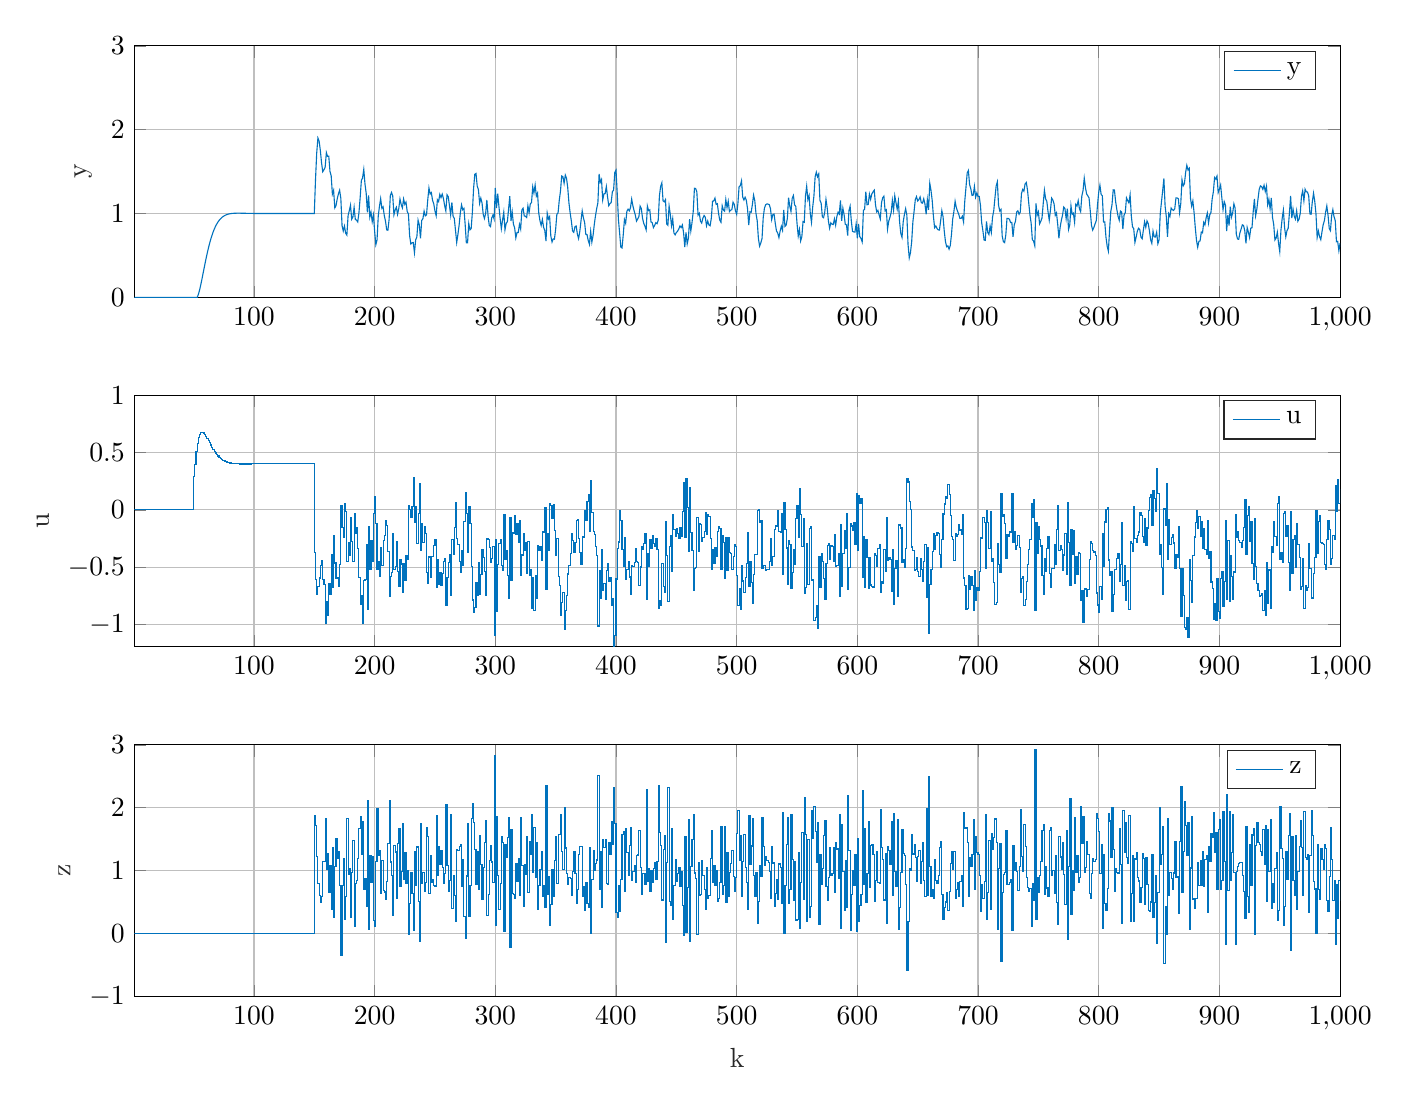
\begin{tikzpicture}

\begin{axis}[%
width=6.028in,
height=1.258in,
at={(1.011in,4.137in)},
scale only axis,
xmin=1,
xmax=1000,
ymin=0,
ymax=3,
ylabel style={font=\color{white!15!black}},
ylabel={y},
axis background/.style={fill=white},
xmajorgrids,
ymajorgrids,
legend style={legend cell align=left, align=left, draw=white!15!black}
]
\addplot [color=mycolor1]
  table[row sep=crcr]{%
1	0\\
2	0\\
3	0\\
4	0\\
5	0\\
6	0\\
7	0\\
8	0\\
9	0\\
10	0\\
11	0\\
12	0\\
13	0\\
14	0\\
15	0\\
16	0\\
17	0\\
18	0\\
19	0\\
20	0\\
21	0\\
22	0\\
23	0\\
24	0\\
25	0\\
26	0\\
27	0\\
28	0\\
29	0\\
30	0\\
31	0\\
32	0\\
33	0\\
34	0\\
35	0\\
36	0\\
37	0\\
38	0\\
39	0\\
40	0\\
41	0\\
42	0\\
43	0\\
44	0\\
45	0\\
46	0\\
47	0\\
48	0\\
49	0\\
50	0\\
51	0\\
52	0\\
53	0\\
54	0.039119\\
55	0.090032\\
56	0.15448\\
57	0.22449\\
58	0.29764\\
59	0.37063\\
60	0.44164\\
61	0.50914\\
62	0.57223\\
63	0.63032\\
64	0.68313\\
65	0.73061\\
66	0.77286\\
67	0.81011\\
68	0.84266\\
69	0.87086\\
70	0.8951\\
71	0.91576\\
72	0.93322\\
73	0.94786\\
74	0.96003\\
75	0.97004\\
76	0.97821\\
77	0.98479\\
78	0.99003\\
79	0.99414\\
80	0.99731\\
81	0.99971\\
82	1.0015\\
83	1.0027\\
84	1.0036\\
85	1.0041\\
86	1.0043\\
87	1.0044\\
88	1.0043\\
89	1.0042\\
90	1.0039\\
91	1.0036\\
92	1.0033\\
93	1.003\\
94	1.0027\\
95	1.0024\\
96	1.0021\\
97	1.0018\\
98	1.0016\\
99	1.0013\\
100	1.0011\\
101	1.001\\
102	1.0008\\
103	1.0007\\
104	1.0005\\
105	1.0004\\
106	1.0003\\
107	1.0003\\
108	1.0002\\
109	1.0002\\
110	1.0001\\
111	1.0001\\
112	1.0001\\
113	1\\
114	1\\
115	1\\
116	1\\
117	0.99999\\
118	0.99998\\
119	0.99998\\
120	0.99998\\
121	0.99998\\
122	0.99998\\
123	0.99998\\
124	0.99998\\
125	0.99998\\
126	0.99998\\
127	0.99998\\
128	0.99998\\
129	0.99998\\
130	0.99998\\
131	0.99998\\
132	0.99999\\
133	0.99999\\
134	0.99999\\
135	0.99999\\
136	0.99999\\
137	0.99999\\
138	0.99999\\
139	0.99999\\
140	0.99999\\
141	0.99999\\
142	0.99999\\
143	0.99999\\
144	0.99999\\
145	0.99999\\
146	0.99999\\
147	0.99999\\
148	0.99999\\
149	0.99999\\
150	0.99999\\
151	1.4011\\
152	1.7216\\
153	1.9007\\
154	1.8641\\
155	1.7543\\
156	1.6074\\
157	1.4983\\
158	1.522\\
159	1.5524\\
160	1.7269\\
161	1.6828\\
162	1.6835\\
163	1.5018\\
164	1.4494\\
165	1.2309\\
166	1.2772\\
167	1.0675\\
168	1.0944\\
169	1.1745\\
170	1.2347\\
171	1.2774\\
172	1.1805\\
173	0.85677\\
174	0.79192\\
175	0.8513\\
176	0.76532\\
177	0.74309\\
178	0.97508\\
179	1.0337\\
180	1.0991\\
181	0.93165\\
182	0.95876\\
183	1.0736\\
184	0.92959\\
185	0.92208\\
186	0.89981\\
187	1.0096\\
188	1.1887\\
189	1.3938\\
190	1.4252\\
191	1.5274\\
192	1.3535\\
193	1.2433\\
194	1.0154\\
195	1.2176\\
196	0.95834\\
197	1.0166\\
198	0.90228\\
199	0.98261\\
200	0.78916\\
201	0.62922\\
202	0.68553\\
203	0.96999\\
204	1.087\\
205	1.1782\\
206	1.062\\
207	1.08\\
208	0.97591\\
209	0.90942\\
210	0.80538\\
211	0.80051\\
212	0.93239\\
213	1.2144\\
214	1.252\\
215	1.2099\\
216	0.98524\\
217	1.0433\\
218	1.0754\\
219	0.99091\\
220	1.0594\\
221	1.1739\\
222	1.1091\\
223	1.0676\\
224	1.1734\\
225	1.1098\\
226	1.1364\\
227	1.0226\\
228	0.99544\\
229	0.7346\\
230	0.63726\\
231	0.65125\\
232	0.65438\\
233	0.533\\
234	0.68621\\
235	0.72172\\
236	0.92118\\
237	0.86578\\
238	0.70312\\
239	0.91681\\
240	0.93774\\
241	1.0302\\
242	0.97217\\
243	0.98494\\
244	1.1605\\
245	1.3049\\
246	1.2324\\
247	1.2495\\
248	1.1571\\
249	1.1151\\
250	1.0304\\
251	0.97422\\
252	1.1639\\
253	1.1425\\
254	1.2288\\
255	1.1902\\
256	1.2318\\
257	1.1806\\
258	1.0943\\
259	1.0318\\
260	1.2239\\
261	1.2006\\
262	1.0955\\
263	0.98227\\
264	1.1334\\
265	0.96805\\
266	0.94135\\
267	0.80234\\
268	0.65487\\
269	0.74859\\
270	0.86073\\
271	1.0057\\
272	1.1044\\
273	1.0453\\
274	1.062\\
275	0.87264\\
276	0.65208\\
277	0.65204\\
278	0.88019\\
279	0.80537\\
280	0.82158\\
281	1.0189\\
282	1.2997\\
283	1.4678\\
284	1.4779\\
285	1.3273\\
286	1.2859\\
287	1.1218\\
288	1.1839\\
289	1.126\\
290	0.98916\\
291	0.94153\\
292	1.0034\\
293	1.161\\
294	0.97077\\
295	0.85776\\
296	0.84342\\
297	0.94552\\
298	0.98022\\
299	0.93444\\
300	1.3069\\
301	1.0662\\
302	1.2366\\
303	1.0835\\
304	0.94044\\
305	0.81944\\
306	0.92138\\
307	1.0166\\
308	0.80568\\
309	0.88261\\
310	0.90359\\
311	1.0541\\
312	1.2061\\
313	0.9117\\
314	1.0191\\
315	0.87277\\
316	0.83113\\
317	0.70999\\
318	0.77451\\
319	0.77258\\
320	0.87057\\
321	0.81542\\
322	1.0426\\
323	1.0634\\
324	0.97085\\
325	0.96797\\
326	0.95321\\
327	1.0919\\
328	1.0094\\
329	1.1168\\
330	1.1317\\
331	1.3179\\
332	1.2455\\
333	1.34\\
334	1.2088\\
335	1.2434\\
336	1.0048\\
337	0.91346\\
338	0.85856\\
339	0.93001\\
340	0.83634\\
341	0.79733\\
342	0.67079\\
343	1.0056\\
344	0.93459\\
345	0.96277\\
346	0.73132\\
347	0.66016\\
348	0.69827\\
349	0.69449\\
350	0.81475\\
351	0.99187\\
352	1.008\\
353	1.1599\\
354	1.2674\\
355	1.4477\\
356	1.4405\\
357	1.3604\\
358	1.4589\\
359	1.4212\\
360	1.3106\\
361	1.1293\\
362	1.0084\\
363	0.91214\\
364	0.79232\\
365	0.77659\\
366	0.84307\\
367	0.85171\\
368	0.75454\\
369	0.70152\\
370	0.78524\\
371	0.91337\\
372	1.0316\\
373	0.94914\\
374	0.89455\\
375	0.7513\\
376	0.74834\\
377	0.67739\\
378	0.63295\\
379	0.78738\\
380	0.6589\\
381	0.73931\\
382	0.8674\\
383	0.97392\\
384	1.0594\\
385	1.1277\\
386	1.4712\\
387	1.3741\\
388	1.4058\\
389	1.1617\\
390	1.2352\\
391	1.2376\\
392	1.3215\\
393	1.1998\\
394	1.0936\\
395	1.1183\\
396	1.1304\\
397	1.261\\
398	1.2783\\
399	1.4897\\
400	1.5188\\
401	1.2482\\
402	0.93269\\
403	0.76838\\
404	0.59849\\
405	0.58998\\
406	0.74488\\
407	0.92878\\
408	0.88321\\
409	1.025\\
410	1.0524\\
411	1.0322\\
412	1.0686\\
413	1.172\\
414	1.0922\\
415	1.0339\\
416	0.9824\\
417	0.91012\\
418	0.93526\\
419	0.96425\\
420	1.0895\\
421	1.0603\\
422	0.94233\\
423	0.88315\\
424	0.84887\\
425	0.80573\\
426	1.0896\\
427	1.0356\\
428	1.0443\\
429	0.9\\
430	0.89209\\
431	0.83238\\
432	0.85782\\
433	0.8913\\
434	0.8788\\
435	0.92212\\
436	1.2134\\
437	1.3246\\
438	1.3663\\
439	1.1514\\
440	1.139\\
441	1.1665\\
442	0.87455\\
443	0.85943\\
444	1.0897\\
445	0.99117\\
446	0.85401\\
447	0.93856\\
448	0.76884\\
449	0.74625\\
450	0.77372\\
451	0.78936\\
452	0.8149\\
453	0.85265\\
454	0.83287\\
455	0.86385\\
456	0.77107\\
457	0.60064\\
458	0.77627\\
459	0.63871\\
460	0.70572\\
461	0.93409\\
462	0.79246\\
463	0.89351\\
464	1.025\\
465	1.3016\\
466	1.2984\\
467	1.2574\\
468	0.98094\\
469	1.004\\
470	0.90992\\
471	0.88711\\
472	0.94492\\
473	0.97649\\
474	0.95675\\
475	0.8546\\
476	0.91014\\
477	0.86333\\
478	0.85386\\
479	0.94623\\
480	1.1477\\
481	1.1502\\
482	1.1841\\
483	1.1098\\
484	1.1172\\
485	0.99909\\
486	0.92167\\
487	0.89568\\
488	1.0921\\
489	1.0416\\
490	1.0275\\
491	1.1673\\
492	1.0695\\
493	1.1471\\
494	1.0234\\
495	1.0405\\
496	1.0469\\
497	1.136\\
498	1.1093\\
499	1.0311\\
500	0.99044\\
501	1.1171\\
502	1.3211\\
503	1.3313\\
504	1.3901\\
505	1.1978\\
506	1.1616\\
507	1.1943\\
508	1.1575\\
509	1.0564\\
510	0.86127\\
511	1.0213\\
512	1.0147\\
513	1.1054\\
514	1.22\\
515	1.1531\\
516	0.99957\\
517	0.91606\\
518	0.70266\\
519	0.61085\\
520	0.65015\\
521	0.70186\\
522	0.95218\\
523	1.0641\\
524	1.1041\\
525	1.1141\\
526	1.1129\\
527	1.1052\\
528	1.0598\\
529	0.92778\\
530	0.98868\\
531	0.99411\\
532	0.88024\\
533	0.79141\\
534	0.76836\\
535	0.71326\\
536	0.79094\\
537	0.8488\\
538	0.80019\\
539	1.0424\\
540	0.84747\\
541	0.86171\\
542	0.94374\\
543	1.1893\\
544	1.088\\
545	1.0244\\
546	1.1809\\
547	1.2156\\
548	1.1033\\
549	1.0841\\
550	0.8831\\
551	0.73169\\
552	0.80957\\
553	0.67309\\
554	0.72473\\
555	0.90541\\
556	0.89694\\
557	1.2083\\
558	1.3257\\
559	1.1659\\
560	1.2151\\
561	0.99975\\
562	0.89486\\
563	1.079\\
564	1.2093\\
565	1.4363\\
566	1.4933\\
567	1.4373\\
568	1.4728\\
569	1.1572\\
570	1.1235\\
571	0.96161\\
572	0.95046\\
573	1.0183\\
574	1.1681\\
575	1.0692\\
576	0.91249\\
577	0.82588\\
578	0.88903\\
579	0.87374\\
580	0.869\\
581	0.93568\\
582	0.86096\\
583	0.96395\\
584	1.0153\\
585	0.99339\\
586	1.1556\\
587	0.91312\\
588	1.0632\\
589	0.98747\\
590	0.87067\\
591	0.86394\\
592	0.737\\
593	1.0328\\
594	1.0881\\
595	0.90978\\
596	0.78698\\
597	0.78113\\
598	0.77804\\
599	0.87961\\
600	0.7043\\
601	0.87595\\
602	0.72431\\
603	0.7045\\
604	0.66048\\
605	1.0387\\
606	1.0499\\
607	1.2594\\
608	1.1042\\
609	1.1084\\
610	1.2311\\
611	1.1698\\
612	1.2347\\
613	1.2583\\
614	1.2795\\
615	1.1082\\
616	1.0209\\
617	1.038\\
618	0.98677\\
619	0.93565\\
620	1.1281\\
621	1.1885\\
622	1.2072\\
623	1.0318\\
624	1.0446\\
625	0.81441\\
626	0.90914\\
627	0.9552\\
628	1.0106\\
629	1.1577\\
630	1.0405\\
631	1.2122\\
632	1.1302\\
633	1.0528\\
634	1.1494\\
635	0.89908\\
636	0.76232\\
637	0.71524\\
638	0.90296\\
639	0.98956\\
640	1.0574\\
641	0.98366\\
642	0.62957\\
643	0.47118\\
644	0.53252\\
645	0.66173\\
646	0.89932\\
647	1.0269\\
648	1.1643\\
649	1.2016\\
650	1.1493\\
651	1.166\\
652	1.1981\\
653	1.1286\\
654	1.1238\\
655	1.176\\
656	1.1144\\
657	0.99173\\
658	1.1653\\
659	1.0455\\
660	1.3615\\
661	1.278\\
662	1.1576\\
663	0.97118\\
664	0.83132\\
665	0.85217\\
666	0.8214\\
667	0.80605\\
668	0.80279\\
669	0.91257\\
670	1.0346\\
671	0.96328\\
672	0.79217\\
673	0.66532\\
674	0.60392\\
675	0.61432\\
676	0.57473\\
677	0.61832\\
678	0.75257\\
679	0.93363\\
680	1.0255\\
681	1.1462\\
682	1.0697\\
683	1.0285\\
684	0.991\\
685	0.94173\\
686	0.94328\\
687	0.96867\\
688	0.89917\\
689	1.1478\\
690	1.3117\\
691	1.4837\\
692	1.5133\\
693	1.3457\\
694	1.2956\\
695	1.2156\\
696	1.2203\\
697	1.3242\\
698	1.1942\\
699	1.2447\\
700	1.2039\\
701	1.2045\\
702	1.0978\\
703	0.89213\\
704	0.79793\\
705	0.68434\\
706	0.6806\\
707	0.90639\\
708	0.7768\\
709	0.75001\\
710	0.85088\\
711	0.77487\\
712	0.95509\\
713	1.0331\\
714	1.1859\\
715	1.3277\\
716	1.3779\\
717	1.0987\\
718	1.0302\\
719	1.0497\\
720	0.73395\\
721	0.66402\\
722	0.65365\\
723	0.74437\\
724	0.94257\\
725	0.94157\\
726	0.93219\\
727	0.89174\\
728	0.8937\\
729	0.72199\\
730	0.86488\\
731	0.90715\\
732	1.0185\\
733	1.032\\
734	0.99176\\
735	1.0174\\
736	1.2394\\
737	1.287\\
738	1.2667\\
739	1.3543\\
740	1.3704\\
741	1.2783\\
742	1.1281\\
743	0.98529\\
744	0.88629\\
745	0.68825\\
746	0.67281\\
747	0.61617\\
748	1.1203\\
749	0.98059\\
750	1.0199\\
751	0.87648\\
752	0.90718\\
753	0.94677\\
754	1.1183\\
755	1.2775\\
756	1.1762\\
757	1.1452\\
758	1.0207\\
759	0.92086\\
760	1.0409\\
761	1.1836\\
762	1.1607\\
763	1.1153\\
764	0.97882\\
765	1.0079\\
766	0.87353\\
767	0.70581\\
768	0.83341\\
769	0.91674\\
770	0.98057\\
771	1.0776\\
772	1.0596\\
773	0.9391\\
774	1.059\\
775	0.81117\\
776	0.86474\\
777	1.0937\\
778	0.99067\\
779	1.0037\\
780	0.8973\\
781	1.1114\\
782	1.0899\\
783	1.1536\\
784	1.0595\\
785	1.0228\\
786	1.2093\\
787	1.2734\\
788	1.4219\\
789	1.3089\\
790	1.2319\\
791	1.2111\\
792	1.1847\\
793	1.0282\\
794	0.86009\\
795	0.80319\\
796	0.83471\\
797	0.87693\\
798	0.91764\\
799	1.1054\\
800	1.2525\\
801	1.3378\\
802	1.2277\\
803	1.2118\\
804	0.89941\\
805	0.90003\\
806	0.71945\\
807	0.60977\\
808	0.55232\\
809	0.80619\\
810	1.0254\\
811	1.1035\\
812	1.2828\\
813	1.2807\\
814	1.1432\\
815	1.0491\\
816	0.96821\\
817	0.92033\\
818	1.0296\\
819	1.018\\
820	0.81341\\
821	0.98323\\
822	1.0108\\
823	1.1877\\
824	1.1542\\
825	1.1277\\
826	1.2236\\
827	0.97159\\
828	0.84119\\
829	0.8204\\
830	0.65489\\
831	0.71921\\
832	0.79028\\
833	0.82463\\
834	0.80852\\
835	0.71802\\
836	0.69888\\
837	0.80325\\
838	0.90221\\
839	0.83584\\
840	0.91191\\
841	0.88158\\
842	0.79653\\
843	0.68795\\
844	0.64525\\
845	0.78974\\
846	0.72206\\
847	0.71926\\
848	0.77722\\
849	0.64037\\
850	0.68469\\
851	1.0016\\
852	1.1401\\
853	1.2737\\
854	1.4179\\
855	1.0903\\
856	0.96418\\
857	0.72229\\
858	0.99879\\
859	0.96646\\
860	1.0653\\
861	1.0462\\
862	1.0381\\
863	1.057\\
864	1.1867\\
865	1.1857\\
866	1.1769\\
867	1.0116\\
868	1.1231\\
869	1.4037\\
870	1.3298\\
871	1.3549\\
872	1.4877\\
873	1.5749\\
874	1.519\\
875	1.5401\\
876	1.1852\\
877	1.089\\
878	1.1514\\
879	1.0125\\
880	0.83383\\
881	0.68179\\
882	0.59805\\
883	0.66827\\
884	0.6739\\
885	0.77903\\
886	0.7701\\
887	0.8949\\
888	0.86471\\
889	0.94809\\
890	1.0065\\
891	0.88833\\
892	0.98458\\
893	1.0136\\
894	1.1743\\
895	1.261\\
896	1.4301\\
897	1.4099\\
898	1.4464\\
899	1.2494\\
900	1.2915\\
901	1.3408\\
902	1.1895\\
903	1.0461\\
904	1.1412\\
905	1.1003\\
906	0.79223\\
907	0.98324\\
908	0.85675\\
909	1.0807\\
910	0.95749\\
911	1.0093\\
912	1.1157\\
913	1.0666\\
914	0.75467\\
915	0.69659\\
916	0.69292\\
917	0.76943\\
918	0.81519\\
919	0.86493\\
920	0.85773\\
921	0.79565\\
922	0.64467\\
923	0.83351\\
924	0.77983\\
925	0.71446\\
926	0.82585\\
927	0.83105\\
928	1.0203\\
929	1.1738\\
930	0.97237\\
931	1.0496\\
932	1.176\\
933	1.2894\\
934	1.3299\\
935	1.3206\\
936	1.2887\\
937	1.3377\\
938	1.2632\\
939	1.3256\\
940	1.104\\
941	1.1705\\
942	1.054\\
943	1.1855\\
944	0.95324\\
945	0.86814\\
946	0.68575\\
947	0.70747\\
948	0.77751\\
949	0.64562\\
950	0.54665\\
951	0.80259\\
952	0.94049\\
953	1.0405\\
954	0.83365\\
955	0.72261\\
956	0.79624\\
957	0.82448\\
958	1.0033\\
959	1.2115\\
960	0.94642\\
961	1.0547\\
962	0.96822\\
963	0.93309\\
964	1.0322\\
965	0.90878\\
966	0.93317\\
967	1.0036\\
968	1.2063\\
969	1.2712\\
970	1.1522\\
971	1.2899\\
972	1.2587\\
973	1.2562\\
974	1.2095\\
975	0.99523\\
976	0.99163\\
977	1.1432\\
978	1.2421\\
979	1.1467\\
980	0.99977\\
981	0.7152\\
982	0.7918\\
983	0.72407\\
984	0.68872\\
985	0.78234\\
986	0.8673\\
987	0.91588\\
988	1.0153\\
989	1.0904\\
990	0.98076\\
991	0.82369\\
992	0.79594\\
993	0.97373\\
994	1.0461\\
995	0.96125\\
996	0.91578\\
997	0.66374\\
998	0.66873\\
999	0.55718\\
1000	0.6479\\
};
\addlegendentry{y}

\end{axis}

\begin{axis}[%
width=6.028in,
height=1.258in,
at={(1.011in,2.39in)},
scale only axis,
xmin=1,
xmax=1000,
ymin=-1.1934,
ymax=1,
ylabel style={font=\color{white!15!black}},
ylabel={u},
axis background/.style={fill=white},
xmajorgrids,
ymajorgrids,
legend style={legend cell align=left, align=left, draw=white!15!black}
]
\addplot[const plot, color=mycolor1] table[row sep=crcr] {%
1	0\\
2	0\\
3	0\\
4	0\\
5	0\\
6	0\\
7	0\\
8	0\\
9	0\\
10	0\\
11	0\\
12	0\\
13	0\\
14	0\\
15	0\\
16	0\\
17	0\\
18	0\\
19	0\\
20	0\\
21	0\\
22	0\\
23	0\\
24	0\\
25	0\\
26	0\\
27	0\\
28	0\\
29	0\\
30	0\\
31	0\\
32	0\\
33	0\\
34	0\\
35	0\\
36	0\\
37	0\\
38	0\\
39	0\\
40	0\\
41	0\\
42	0\\
43	0\\
44	0\\
45	0\\
46	0\\
47	0\\
48	0\\
49	0\\
50	0.28956\\
51	0.39251\\
52	0.5131\\
53	0.58007\\
54	0.63135\\
55	0.65951\\
56	0.67407\\
57	0.67664\\
58	0.67103\\
59	0.65931\\
60	0.64358\\
61	0.62529\\
62	0.60567\\
63	0.58562\\
64	0.56581\\
65	0.54674\\
66	0.52873\\
67	0.512\\
68	0.49669\\
69	0.48283\\
70	0.47042\\
71	0.45942\\
72	0.44977\\
73	0.44136\\
74	0.4341\\
75	0.42788\\
76	0.4226\\
77	0.41815\\
78	0.41444\\
79	0.41136\\
80	0.40884\\
81	0.4068\\
82	0.40516\\
83	0.40387\\
84	0.40286\\
85	0.40209\\
86	0.40151\\
87	0.4011\\
88	0.40081\\
89	0.40063\\
90	0.40052\\
91	0.40048\\
92	0.40048\\
93	0.40051\\
94	0.40057\\
95	0.40065\\
96	0.40073\\
97	0.40082\\
98	0.40091\\
99	0.401\\
100	0.40108\\
101	0.40116\\
102	0.40123\\
103	0.4013\\
104	0.40136\\
105	0.40142\\
106	0.40146\\
107	0.4015\\
108	0.40154\\
109	0.40157\\
110	0.4016\\
111	0.40162\\
112	0.40164\\
113	0.40166\\
114	0.40167\\
115	0.40168\\
116	0.40169\\
117	0.4017\\
118	0.4017\\
119	0.40171\\
120	0.40171\\
121	0.40171\\
122	0.40171\\
123	0.40172\\
124	0.40172\\
125	0.40172\\
126	0.40172\\
127	0.40172\\
128	0.40172\\
129	0.40172\\
130	0.40172\\
131	0.40172\\
132	0.40172\\
133	0.40171\\
134	0.40171\\
135	0.40171\\
136	0.40171\\
137	0.40171\\
138	0.40171\\
139	0.40171\\
140	0.40171\\
141	0.40171\\
142	0.40171\\
143	0.40171\\
144	0.40171\\
145	0.40171\\
146	0.40171\\
147	0.40171\\
148	0.40171\\
149	0.40171\\
150	-0.36978\\
151	-0.60501\\
152	-0.73331\\
153	-0.669\\
154	-0.59341\\
155	-0.48146\\
156	-0.44093\\
157	-0.60541\\
158	-0.65017\\
159	-0.99382\\
160	-0.80207\\
161	-0.92197\\
162	-0.64514\\
163	-0.73808\\
164	-0.38957\\
165	-0.67747\\
166	-0.22533\\
167	-0.46257\\
168	-0.59608\\
169	-0.59193\\
170	-0.66974\\
171	-0.47368\\
172	0.036542\\
173	-0.15018\\
174	-0.24419\\
175	0.051928\\
176	-0.010464\\
177	-0.45098\\
178	-0.28804\\
179	-0.401\\
180	-0.068991\\
181	-0.27167\\
182	-0.45125\\
183	-0.030604\\
184	-0.20135\\
185	-0.15268\\
186	-0.33282\\
187	-0.58717\\
188	-0.81974\\
189	-0.74412\\
190	-0.99135\\
191	-0.61387\\
192	-0.60875\\
193	-0.30136\\
194	-0.86553\\
195	-0.14817\\
196	-0.52012\\
197	-0.26415\\
198	-0.45317\\
199	-0.030436\\
200	0.11718\\
201	-0.12188\\
202	-0.51812\\
203	-0.4508\\
204	-0.58035\\
205	-0.32819\\
206	-0.48532\\
207	-0.27033\\
208	-0.22254\\
209	-0.0892\\
210	-0.13776\\
211	-0.36585\\
212	-0.75516\\
213	-0.58107\\
214	-0.54324\\
215	-0.20957\\
216	-0.51964\\
217	-0.49225\\
218	-0.27849\\
219	-0.53781\\
220	-0.67052\\
221	-0.4307\\
222	-0.47156\\
223	-0.72074\\
224	-0.47003\\
225	-0.61835\\
226	-0.39632\\
227	-0.43577\\
228	0.035964\\
229	0.0053332\\
230	-0.063914\\
231	0.032601\\
232	0.28095\\
233	-0.1098\\
234	0.030502\\
235	-0.29646\\
236	-0.029412\\
237	0.22796\\
238	-0.35626\\
239	-0.11641\\
240	-0.28082\\
241	-0.14417\\
242	-0.20578\\
243	-0.54337\\
244	-0.6398\\
245	-0.4106\\
246	-0.58932\\
247	-0.40559\\
248	-0.40984\\
249	-0.30745\\
250	-0.26049\\
251	-0.67242\\
252	-0.43026\\
253	-0.65317\\
254	-0.54546\\
255	-0.65911\\
256	-0.55609\\
257	-0.44613\\
258	-0.42648\\
259	-0.83621\\
260	-0.59232\\
261	-0.456\\
262	-0.38927\\
263	-0.74595\\
264	-0.25684\\
265	-0.3894\\
266	-0.15627\\
267	0.060023\\
268	-0.24733\\
269	-0.30023\\
270	-0.45017\\
271	-0.54252\\
272	-0.35573\\
273	-0.48031\\
274	-0.10149\\
275	0.15564\\
276	-0.033047\\
277	-0.37411\\
278	0.030094\\
279	-0.12049\\
280	-0.48965\\
281	-0.78552\\
282	-0.89636\\
283	-0.85334\\
284	-0.63642\\
285	-0.74269\\
286	-0.4628\\
287	-0.7327\\
288	-0.56159\\
289	-0.34528\\
290	-0.41578\\
291	-0.53572\\
292	-0.74966\\
293	-0.25348\\
294	-0.26112\\
295	-0.32891\\
296	-0.45785\\
297	-0.42378\\
298	-0.31938\\
299	-1.0937\\
300	-0.25925\\
301	-0.88307\\
302	-0.47481\\
303	-0.28968\\
304	-0.25481\\
305	-0.4872\\
306	-0.53176\\
307	-0.044323\\
308	-0.43094\\
309	-0.35255\\
310	-0.57542\\
311	-0.7686\\
312	-0.068503\\
313	-0.61606\\
314	-0.19808\\
315	-0.20132\\
316	-0.045218\\
317	-0.21352\\
318	-0.11817\\
319	-0.28581\\
320	-0.089599\\
321	-0.5714\\
322	-0.39322\\
323	-0.20998\\
324	-0.35266\\
325	-0.28514\\
326	-0.54966\\
327	-0.27183\\
328	-0.57503\\
329	-0.51857\\
330	-0.85459\\
331	-0.58627\\
332	-0.87636\\
333	-0.57637\\
334	-0.77326\\
335	-0.31149\\
336	-0.34965\\
337	-0.32096\\
338	-0.44016\\
339	-0.18552\\
340	-0.20001\\
341	0.020544\\
342	-0.69491\\
343	-0.2034\\
344	-0.35208\\
345	0.05986\\
346	0.037954\\
347	-0.074323\\
348	0.048057\\
349	-0.18086\\
350	-0.39531\\
351	-0.24853\\
352	-0.57672\\
353	-0.66026\\
354	-0.92137\\
355	-0.80843\\
356	-0.72356\\
357	-1.0455\\
358	-0.87849\\
359	-0.74363\\
360	-0.55875\\
361	-0.48125\\
362	-0.38285\\
363	-0.20958\\
364	-0.2668\\
365	-0.36681\\
366	-0.28471\\
367	-0.09555\\
368	-0.084003\\
369	-0.25245\\
370	-0.37218\\
371	-0.47662\\
372	-0.23514\\
373	-0.23703\\
374	-0.0062523\\
375	-0.095658\\
376	0.071667\\
377	0.1311\\
378	-0.18798\\
379	0.25708\\
380	-0.024963\\
381	-0.18484\\
382	-0.21156\\
383	-0.32198\\
384	-0.39767\\
385	-1.0115\\
386	-0.53002\\
387	-0.77517\\
388	-0.34958\\
389	-0.69867\\
390	-0.6442\\
391	-0.78421\\
392	-0.53098\\
393	-0.46515\\
394	-0.62489\\
395	-0.58719\\
396	-0.83666\\
397	-0.77281\\
398	-1.1934\\
399	-1.0957\\
400	-0.60212\\
401	-0.33663\\
402	-0.27964\\
403	-0.0093514\\
404	-0.094659\\
405	-0.34349\\
406	-0.49087\\
407	-0.24463\\
408	-0.60424\\
409	-0.51631\\
410	-0.44673\\
411	-0.5846\\
412	-0.73258\\
413	-0.48648\\
414	-0.49308\\
415	-0.45648\\
416	-0.33315\\
417	-0.44677\\
418	-0.45737\\
419	-0.65785\\
420	-0.49776\\
421	-0.32209\\
422	-0.3402\\
423	-0.28921\\
424	-0.20732\\
425	-0.78327\\
426	-0.38354\\
427	-0.49256\\
428	-0.26034\\
429	-0.33617\\
430	-0.21955\\
431	-0.29108\\
432	-0.32247\\
433	-0.24693\\
434	-0.3487\\
435	-0.85908\\
436	-0.78931\\
437	-0.83436\\
438	-0.47055\\
439	-0.66792\\
440	-0.71866\\
441	-0.10259\\
442	-0.39361\\
443	-0.79946\\
444	-0.3159\\
445	-0.22636\\
446	-0.53789\\
447	-0.044153\\
448	-0.17027\\
449	-0.23487\\
450	-0.1616\\
451	-0.20548\\
452	-0.24452\\
453	-0.15259\\
454	-0.23208\\
455	-0.012732\\
456	0.24137\\
457	-0.23857\\
458	0.26954\\
459	0.020521\\
460	-0.36192\\
461	0.19783\\
462	-0.19597\\
463	-0.35138\\
464	-0.70427\\
465	-0.50823\\
466	-0.50419\\
467	-0.0667\\
468	-0.36187\\
469	-0.12166\\
470	-0.12819\\
471	-0.27869\\
472	-0.24321\\
473	-0.18524\\
474	-0.025277\\
475	-0.21688\\
476	-0.043742\\
477	-0.057106\\
478	-0.24926\\
479	-0.51617\\
480	-0.34451\\
481	-0.46686\\
482	-0.32656\\
483	-0.4082\\
484	-0.18737\\
485	-0.1443\\
486	-0.16142\\
487	-0.52323\\
488	-0.22776\\
489	-0.28651\\
490	-0.59968\\
491	-0.24225\\
492	-0.52903\\
493	-0.2378\\
494	-0.36871\\
495	-0.38364\\
496	-0.51959\\
497	-0.40622\\
498	-0.30272\\
499	-0.31568\\
500	-0.57446\\
501	-0.83139\\
502	-0.68707\\
503	-0.86876\\
504	-0.48868\\
505	-0.61953\\
506	-0.72322\\
507	-0.58582\\
508	-0.46463\\
509	-0.19784\\
510	-0.66326\\
511	-0.4491\\
512	-0.62937\\
513	-0.81348\\
514	-0.56554\\
515	-0.38796\\
516	-0.38852\\
517	-0.0059637\\
518	-0.00018991\\
519	-0.11237\\
520	-0.093481\\
521	-0.51199\\
522	-0.48572\\
523	-0.48523\\
524	-0.52997\\
525	-0.52146\\
526	-0.51902\\
527	-0.45227\\
528	-0.24686\\
529	-0.4874\\
530	-0.40889\\
531	-0.17375\\
532	-0.13922\\
533	-0.14117\\
534	-0.0070726\\
535	-0.18959\\
536	-0.19877\\
537	-0.033216\\
538	-0.56377\\
539	0.065085\\
540	-0.17045\\
541	-0.3317\\
542	-0.64616\\
543	-0.26276\\
544	-0.29861\\
545	-0.6806\\
546	-0.54807\\
547	-0.34728\\
548	-0.47553\\
549	-0.077973\\
550	0.035764\\
551	-0.23642\\
552	0.18417\\
553	-0.038556\\
554	-0.32183\\
555	-0.074165\\
556	-0.7313\\
557	-0.67655\\
558	-0.28935\\
559	-0.64796\\
560	-0.15822\\
561	-0.14779\\
562	-0.61355\\
563	-0.61031\\
564	-0.9643\\
565	-0.93871\\
566	-0.83265\\
567	-1.0337\\
568	-0.4074\\
569	-0.67181\\
570	-0.37868\\
571	-0.44778\\
572	-0.59915\\
573	-0.7812\\
574	-0.47077\\
575	-0.30971\\
576	-0.29637\\
577	-0.43533\\
578	-0.3095\\
579	-0.31663\\
580	-0.45084\\
581	-0.21758\\
582	-0.49448\\
583	-0.4871\\
584	-0.38271\\
585	-0.75624\\
586	-0.12597\\
587	-0.67021\\
588	-0.37942\\
589	-0.18365\\
590	-0.33614\\
591	-0.032073\\
592	-0.69716\\
593	-0.5034\\
594	-0.12039\\
595	-0.14041\\
596	-0.18115\\
597	-0.11367\\
598	-0.30478\\
599	0.14188\\
600	-0.35382\\
601	0.12745\\
602	0.052683\\
603	0.1022\\
604	-0.58582\\
605	-0.23476\\
606	-0.67994\\
607	-0.25809\\
608	-0.41674\\
609	-0.68638\\
610	-0.41105\\
611	-0.65409\\
612	-0.66539\\
613	-0.67836\\
614	-0.38096\\
615	-0.39566\\
616	-0.49528\\
617	-0.339\\
618	-0.30121\\
619	-0.72013\\
620	-0.62287\\
621	-0.63778\\
622	-0.34682\\
623	-0.53771\\
624	-0.062551\\
625	-0.43882\\
626	-0.41388\\
627	-0.43207\\
628	-0.71193\\
629	-0.3449\\
630	-0.82183\\
631	-0.51396\\
632	-0.44157\\
633	-0.75296\\
634	-0.13181\\
635	-0.13039\\
636	-0.1573\\
637	-0.4573\\
638	-0.42919\\
639	-0.49975\\
640	-0.33414\\
641	0.27123\\
642	0.24355\\
643	0.071722\\
644	9.9164e-05\\
645	-0.32337\\
646	-0.35364\\
647	-0.52866\\
648	-0.5224\\
649	-0.41698\\
650	-0.53736\\
651	-0.58395\\
652	-0.42512\\
653	-0.51612\\
654	-0.62291\\
655	-0.44699\\
656	-0.30225\\
657	-0.76072\\
658	-0.32688\\
659	-1.075\\
660	-0.64748\\
661	-0.51567\\
662	-0.36203\\
663	-0.20637\\
664	-0.34477\\
665	-0.21914\\
666	-0.19746\\
667	-0.20384\\
668	-0.3856\\
669	-0.50094\\
670	-0.25813\\
671	-0.035102\\
672	0.051379\\
673	0.11522\\
674	0.097075\\
675	0.22525\\
676	0.13498\\
677	-0.048382\\
678	-0.23525\\
679	-0.2542\\
680	-0.43838\\
681	-0.20879\\
682	-0.23079\\
683	-0.21151\\
684	-0.12368\\
685	-0.17536\\
686	-0.20982\\
687	-0.040596\\
688	-0.59388\\
689	-0.65833\\
690	-0.86381\\
691	-0.86307\\
692	-0.5695\\
693	-0.69427\\
694	-0.58503\\
695	-0.65519\\
696	-0.87205\\
697	-0.52553\\
698	-0.79311\\
699	-0.68052\\
700	-0.70582\\
701	-0.54068\\
702	-0.24352\\
703	-0.25239\\
704	-0.066738\\
705	-0.11087\\
706	-0.51381\\
707	-0.005851\\
708	-0.11055\\
709	-0.33296\\
710	-0.010129\\
711	-0.45327\\
712	-0.42445\\
713	-0.63121\\
714	-0.82357\\
715	-0.8105\\
716	-0.2925\\
717	-0.47688\\
718	-0.54133\\
719	0.14325\\
720	-0.056907\\
721	-0.039672\\
722	-0.11951\\
723	-0.42035\\
724	-0.21843\\
725	-0.23453\\
726	-0.18993\\
727	-0.20059\\
728	0.13896\\
729	-0.28744\\
730	-0.19\\
731	-0.34184\\
732	-0.31111\\
733	-0.22121\\
734	-0.33123\\
735	-0.72235\\
736	-0.60054\\
737	-0.57977\\
738	-0.83287\\
739	-0.77816\\
740	-0.62527\\
741	-0.479\\
742	-0.34337\\
743	-0.26147\\
744	0.059778\\
745	-0.064054\\
746	0.088873\\
747	-0.87689\\
748	-0.11023\\
749	-0.38302\\
750	-0.14662\\
751	-0.25447\\
752	-0.3141\\
753	-0.57538\\
754	-0.73603\\
755	-0.42762\\
756	-0.53326\\
757	-0.33243\\
758	-0.23155\\
759	-0.55725\\
760	-0.67482\\
761	-0.50936\\
762	-0.51192\\
763	-0.30605\\
764	-0.47466\\
765	-0.17018\\
766	0.040877\\
767	-0.35508\\
768	-0.3138\\
769	-0.34848\\
770	-0.5235\\
771	-0.3926\\
772	-0.20239\\
773	-0.56621\\
774	0.062573\\
775	-0.28185\\
776	-0.66094\\
777	-0.17379\\
778	-0.38388\\
779	-0.18178\\
780	-0.64166\\
781	-0.40442\\
782	-0.56293\\
783	-0.37458\\
784	-0.38165\\
785	-0.78657\\
786	-0.70726\\
787	-0.9788\\
788	-0.68978\\
789	-0.68563\\
790	-0.75337\\
791	-0.69366\\
792	-0.43458\\
793	-0.27526\\
794	-0.29614\\
795	-0.35008\\
796	-0.36639\\
797	-0.4008\\
798	-0.72409\\
799	-0.8284\\
800	-0.8906\\
801	-0.66892\\
802	-0.78417\\
803	-0.20316\\
804	-0.49094\\
805	-0.10506\\
806	0.0023444\\
807	0.016737\\
808	-0.4364\\
809	-0.57185\\
810	-0.53678\\
811	-0.88665\\
812	-0.73642\\
813	-0.51572\\
814	-0.52196\\
815	-0.42492\\
816	-0.38101\\
817	-0.62724\\
818	-0.47821\\
819	-0.11112\\
820	-0.65667\\
821	-0.48489\\
822	-0.78899\\
823	-0.62241\\
824	-0.61509\\
825	-0.86482\\
826	-0.27219\\
827	-0.29385\\
828	-0.36337\\
829	0.029975\\
830	-0.24809\\
831	-0.27977\\
832	-0.22637\\
833	-0.19291\\
834	-0.02404\\
835	-0.051444\\
836	-0.23485\\
837	-0.28578\\
838	-0.071824\\
839	-0.30714\\
840	-0.15742\\
841	-0.0065514\\
842	0.10574\\
843	0.13034\\
844	-0.13863\\
845	0.16814\\
846	0.10256\\
847	-0.0097228\\
848	0.3637\\
849	0.14202\\
850	-0.39038\\
851	-0.30159\\
852	-0.50475\\
853	-0.73588\\
854	0.0085047\\
855	-0.13604\\
856	0.23013\\
857	-0.43338\\
858	-0.082279\\
859	-0.30439\\
860	-0.23986\\
861	-0.21424\\
862	-0.28856\\
863	-0.51117\\
864	-0.3922\\
865	-0.41711\\
866	-0.14197\\
867	-0.50909\\
868	-0.92428\\
869	-0.51306\\
870	-0.74357\\
871	-1.0221\\
872	-1.0441\\
873	-0.9394\\
874	-1.1101\\
875	-0.43285\\
876	-0.61562\\
877	-0.80577\\
878	-0.39894\\
879	-0.23638\\
880	-0.10669\\
881	-0.0052713\\
882	-0.1639\\
883	-0.054327\\
884	-0.22776\\
885	-0.10397\\
886	-0.33697\\
887	-0.1613\\
888	-0.34536\\
889	-0.39003\\
890	-0.094387\\
891	-0.42325\\
892	-0.36362\\
893	-0.62877\\
894	-0.68705\\
895	-0.95445\\
896	-0.81517\\
897	-0.96189\\
898	-0.60136\\
899	-0.88889\\
900	-0.95003\\
901	-0.60047\\
902	-0.53535\\
903	-0.84521\\
904	-0.62125\\
905	-0.090812\\
906	-0.78244\\
907	-0.26735\\
908	-0.79554\\
909	-0.39403\\
910	-0.58346\\
911	-0.77946\\
912	-0.54135\\
913	-0.038168\\
914	-0.23564\\
915	-0.19218\\
916	-0.26639\\
917	-0.28742\\
918	-0.32512\\
919	-0.2654\\
920	-0.15116\\
921	0.087837\\
922	-0.38879\\
923	-0.048536\\
924	0.031387\\
925	-0.27371\\
926	-0.1053\\
927	-0.46814\\
928	-0.60479\\
929	-0.079468\\
930	-0.4956\\
931	-0.64149\\
932	-0.70135\\
933	-0.75553\\
934	-0.7441\\
935	-0.72574\\
936	-0.87739\\
937	-0.70207\\
938	-0.92319\\
939	-0.46101\\
940	-0.8113\\
941	-0.52374\\
942	-0.85822\\
943	-0.31603\\
944	-0.36896\\
945	-0.099082\\
946	-0.23032\\
947	-0.30927\\
948	0.058446\\
949	0.11222\\
950	-0.43329\\
951	-0.36939\\
952	-0.45564\\
953	-0.03412\\
954	-0.018433\\
955	-0.23408\\
956	-0.13935\\
957	-0.45998\\
958	-0.70392\\
959	-0.010252\\
960	-0.55127\\
961	-0.25831\\
962	-0.22056\\
963	-0.49774\\
964	-0.1169\\
965	-0.30075\\
966	-0.41694\\
967	-0.69581\\
968	-0.66494\\
969	-0.42737\\
970	-0.8606\\
971	-0.65556\\
972	-0.69922\\
973	-0.6738\\
974	-0.29547\\
975	-0.50867\\
976	-0.76779\\
977	-0.77483\\
978	-0.55768\\
979	-0.41844\\
980	-0.0023109\\
981	-0.37612\\
982	-0.099975\\
983	-0.052614\\
984	-0.28023\\
985	-0.29107\\
986	-0.30202\\
987	-0.4732\\
988	-0.52096\\
989	-0.25586\\
990	-0.093015\\
991	-0.17347\\
992	-0.4793\\
993	-0.41997\\
994	-0.2237\\
995	-0.25991\\
996	0.20813\\
997	-0.010567\\
998	0.26238\\
999	0.052221\\
1000	0.17927\\
};
\addlegendentry{u}

\end{axis}

\begin{axis}[%
width=6.028in,
height=1.258in,
at={(1.011in,0.642in)},
scale only axis,
xmin=1,
xmax=1000,
xlabel style={font=\color{white!15!black}},
xlabel={k},
ymin=-1,
ymax=3,
ylabel style={font=\color{white!15!black}},
ylabel={z},
axis background/.style={fill=white},
xmajorgrids,
ymajorgrids,
legend style={legend cell align=left, align=left, draw=white!15!black}
]
\addplot[const plot, color=mycolor1] table[row sep=crcr] {%
1	0\\
2	0\\
3	0\\
4	0\\
5	0\\
6	0\\
7	0\\
8	0\\
9	0\\
10	0\\
11	0\\
12	0\\
13	0\\
14	0\\
15	0\\
16	0\\
17	0\\
18	0\\
19	0\\
20	0\\
21	0\\
22	0\\
23	0\\
24	0\\
25	0\\
26	0\\
27	0\\
28	0\\
29	0\\
30	0\\
31	0\\
32	0\\
33	0\\
34	0\\
35	0\\
36	0\\
37	0\\
38	0\\
39	0\\
40	0\\
41	0\\
42	0\\
43	0\\
44	0\\
45	0\\
46	0\\
47	0\\
48	0\\
49	0\\
50	0\\
51	0\\
52	0\\
53	0\\
54	0\\
55	0\\
56	0\\
57	0\\
58	0\\
59	0\\
60	0\\
61	0\\
62	0\\
63	0\\
64	0\\
65	0\\
66	0\\
67	0\\
68	0\\
69	0\\
70	0\\
71	0\\
72	0\\
73	0\\
74	0\\
75	0\\
76	0\\
77	0\\
78	0\\
79	0\\
80	0\\
81	0\\
82	0\\
83	0\\
84	0\\
85	0\\
86	0\\
87	0\\
88	0\\
89	0\\
90	0\\
91	0\\
92	0\\
93	0\\
94	0\\
95	0\\
96	0\\
97	0\\
98	0\\
99	0\\
100	0\\
101	0\\
102	0\\
103	0\\
104	0\\
105	0\\
106	0\\
107	0\\
108	0\\
109	0\\
110	0\\
111	0\\
112	0\\
113	0\\
114	0\\
115	0\\
116	0\\
117	0\\
118	0\\
119	0\\
120	0\\
121	0\\
122	0\\
123	0\\
124	0\\
125	0\\
126	0\\
127	0\\
128	0\\
129	0\\
130	0\\
131	0\\
132	0\\
133	0\\
134	0\\
135	0\\
136	0\\
137	0\\
138	0\\
139	0\\
140	0\\
141	0\\
142	0\\
143	0\\
144	0\\
145	0\\
146	0\\
147	0\\
148	0\\
149	0\\
150	1.881\\
151	1.7139\\
152	1.2199\\
153	0.79098\\
154	0.60651\\
155	0.49148\\
156	0.589\\
157	1.1402\\
158	1.1431\\
159	1.8323\\
160	1.0243\\
161	1.2652\\
162	0.65379\\
163	1.0809\\
164	0.37815\\
165	1.3605\\
166	0.26256\\
167	1.0627\\
168	1.5159\\
169	1.1965\\
170	1.2962\\
171	0.75772\\
172	-0.3463\\
173	0.75898\\
174	1.1978\\
175	0.23079\\
176	0.59018\\
177	1.8251\\
178	0.94516\\
179	1.0357\\
180	0.24783\\
181	0.97648\\
182	1.4747\\
183	0.11654\\
184	0.80187\\
185	0.84307\\
186	1.1915\\
187	1.6734\\
188	1.857\\
189	1.2611\\
190	1.7736\\
191	0.69276\\
192	0.87216\\
193	0.43549\\
194	2.1181\\
195	0.066511\\
196	1.2329\\
197	0.80881\\
198	1.2247\\
199	0.20922\\
200	0.1071\\
201	1.1517\\
202	1.9856\\
203	1.2429\\
204	1.3168\\
205	0.63531\\
206	1.1669\\
207	0.69013\\
208	0.66022\\
209	0.54732\\
210	0.82595\\
211	1.4306\\
212	2.1146\\
213	1.1374\\
214	0.92071\\
215	0.29031\\
216	1.4033\\
217	1.2963\\
218	0.56148\\
219	1.4249\\
220	1.6646\\
221	0.75308\\
222	0.98869\\
223	1.7478\\
224	0.86718\\
225	1.284\\
226	0.80016\\
227	0.99896\\
228	-0.015296\\
229	0.48054\\
230	0.97485\\
231	0.63243\\
232	0.052295\\
233	1.3046\\
234	0.76024\\
235	1.3756\\
236	0.50983\\
237	-0.11868\\
238	1.7554\\
239	0.79519\\
240	0.96906\\
241	0.66394\\
242	0.81754\\
243	1.6866\\
244	1.5483\\
245	0.6421\\
246	1.237\\
247	0.80447\\
248	0.86157\\
249	0.7573\\
250	0.74148\\
251	1.8715\\
252	0.92055\\
253	1.3842\\
254	1.103\\
255	1.319\\
256	1.0511\\
257	0.80282\\
258	0.9483\\
259	2.0548\\
260	1.083\\
261	0.67683\\
262	0.84428\\
263	1.8862\\
264	0.40185\\
265	0.92389\\
266	0.60771\\
267	0.19682\\
268	1.3273\\
269	1.3138\\
270	1.3796\\
271	1.416\\
272	0.75631\\
273	1.1728\\
274	0.27633\\
275	-0.081948\\
276	0.91367\\
277	1.7471\\
278	0.27276\\
279	0.76009\\
280	1.8222\\
281	2.0631\\
282	1.7649\\
283	1.3384\\
284	0.78503\\
285	1.3052\\
286	0.70156\\
287	1.5565\\
288	1.1025\\
289	0.53663\\
290	1.0554\\
291	1.4465\\
292	1.7953\\
293	0.28813\\
294	0.62485\\
295	1.167\\
296	1.4022\\
297	1.1369\\
298	0.81356\\
299	2.8281\\
300	0.12818\\
301	1.8627\\
302	0.92115\\
303	0.3839\\
304	0.79945\\
305	1.5383\\
306	1.4428\\
307	0.028566\\
308	1.4066\\
309	1.2141\\
310	1.5262\\
311	1.8422\\
312	-0.22106\\
313	1.6459\\
314	0.6404\\
315	0.62275\\
316	0.56044\\
317	1.1091\\
318	0.82419\\
319	1.1842\\
320	0.61037\\
321	1.8378\\
322	1.0859\\
323	0.4377\\
324	1.1043\\
325	0.94205\\
326	1.5389\\
327	0.65856\\
328	1.4629\\
329	1.2509\\
330	1.8927\\
331	0.96648\\
332	1.6837\\
333	0.89305\\
334	1.4488\\
335	0.37619\\
336	0.76851\\
337	1.0208\\
338	1.3038\\
339	0.58562\\
340	0.77043\\
341	0.4101\\
342	2.3456\\
343	0.61807\\
344	0.89775\\
345	0.1322\\
346	0.46169\\
347	1.0232\\
348	0.5841\\
349	1.1607\\
350	1.5467\\
351	0.79739\\
352	1.573\\
353	1.5763\\
354	1.884\\
355	1.3055\\
356	1.0231\\
357	1.9957\\
358	1.3591\\
359	0.95953\\
360	0.78631\\
361	0.89109\\
362	0.87355\\
363	0.60537\\
364	0.98393\\
365	1.2985\\
366	0.94852\\
367	0.48305\\
368	0.69479\\
369	1.2528\\
370	1.379\\
371	1.3796\\
372	0.59524\\
373	0.75257\\
374	0.37329\\
375	0.80566\\
376	0.48037\\
377	0.41542\\
378	1.3673\\
379	0.00597\\
380	0.86479\\
381	1.3159\\
382	0.99604\\
383	1.1116\\
384	1.1688\\
385	2.5094\\
386	0.69279\\
387	1.2966\\
388	0.41426\\
389	1.4977\\
390	1.367\\
391	1.4977\\
392	0.79965\\
393	0.78666\\
394	1.4443\\
395	1.2527\\
396	1.7783\\
397	1.4187\\
398	2.323\\
399	1.7432\\
400	0.3278\\
401	0.25341\\
402	0.76119\\
403	0.35758\\
404	0.85909\\
405	1.5772\\
406	1.6142\\
407	0.67028\\
408	1.668\\
409	1.295\\
410	0.9311\\
411	1.4061\\
412	1.6891\\
413	0.84265\\
414	0.98811\\
415	1.0875\\
416	0.81687\\
417	1.24\\
418	1.2485\\
419	1.636\\
420	1.0443\\
421	0.61814\\
422	0.95832\\
423	0.94939\\
424	0.77908\\
425	2.2955\\
426	0.82329\\
427	1.0302\\
428	0.67314\\
429	0.99605\\
430	0.81517\\
431	1.0372\\
432	1.129\\
433	0.85294\\
434	1.1452\\
435	2.3455\\
436	1.603\\
437	1.3937\\
438	0.53305\\
439	1.3428\\
440	1.5649\\
441	-0.13493\\
442	1.1347\\
443	2.317\\
444	0.51444\\
445	0.45163\\
446	1.6733\\
447	0.23131\\
448	0.76888\\
449	1.1799\\
450	0.82877\\
451	0.94772\\
452	1.0493\\
453	0.74569\\
454	0.99164\\
455	0.44495\\
456	-0.031776\\
457	1.5431\\
458	0.022627\\
459	0.73548\\
460	1.8098\\
461	-0.12977\\
462	1.07\\
463	1.4973\\
464	1.8959\\
465	0.96162\\
466	0.87929\\
467	-0.018333\\
468	1.1334\\
469	0.60201\\
470	0.61784\\
471	1.1624\\
472	0.92049\\
473	0.69451\\
474	0.38741\\
475	1.051\\
476	0.56249\\
477	0.60845\\
478	1.1936\\
479	1.6426\\
480	0.81689\\
481	1.0802\\
482	0.76079\\
483	1.0061\\
484	0.50293\\
485	0.55064\\
486	0.8051\\
487	1.6999\\
488	0.61454\\
489	0.76527\\
490	1.7047\\
491	0.48662\\
492	1.2937\\
493	0.58946\\
494	0.97026\\
495	1.109\\
496	1.3249\\
497	0.90921\\
498	0.66613\\
499	0.89005\\
500	1.5894\\
501	1.9566\\
502	1.1627\\
503	1.5598\\
504	0.5852\\
505	1.1435\\
506	1.5741\\
507	1.043\\
508	0.80815\\
509	0.38761\\
510	1.8742\\
511	1.1059\\
512	1.3906\\
513	1.8356\\
514	0.91818\\
515	0.5908\\
516	0.96189\\
517	0.16493\\
518	0.51365\\
519	1.0771\\
520	0.91042\\
521	1.8482\\
522	1.3856\\
523	1.0836\\
524	1.2181\\
525	1.1586\\
526	1.1306\\
527	0.98143\\
528	0.55064\\
529	1.3883\\
530	1.1217\\
531	0.43611\\
532	0.63949\\
533	0.85414\\
534	0.54243\\
535	1.1052\\
536	1.0446\\
537	0.48161\\
538	1.9217\\
539	-0.00094849\\
540	0.76693\\
541	1.4171\\
542	1.8375\\
543	0.47483\\
544	0.69512\\
545	1.8937\\
546	1.1748\\
547	0.52418\\
548	1.1428\\
549	0.20912\\
550	0.21652\\
551	1.2931\\
552	0.081523\\
553	0.80951\\
554	1.6002\\
555	0.53862\\
556	2.1566\\
557	1.5811\\
558	0.18776\\
559	1.4926\\
560	0.26004\\
561	0.43366\\
562	1.9602\\
563	1.5065\\
564	2.0154\\
565	1.6267\\
566	1.1361\\
567	1.7698\\
568	0.14935\\
569	1.2584\\
570	0.7824\\
571	1.0297\\
572	1.5597\\
573	1.8017\\
574	0.7545\\
575	0.52686\\
576	0.89326\\
577	1.3646\\
578	0.92726\\
579	0.95367\\
580	1.3673\\
581	0.6584\\
582	1.4511\\
583	1.343\\
584	0.87854\\
585	1.8973\\
586	0.082434\\
587	1.7309\\
588	0.98577\\
589	0.36552\\
590	1.1528\\
591	0.40975\\
592	2.1987\\
593	1.3135\\
594	0.050478\\
595	0.62395\\
596	0.99564\\
597	0.76582\\
598	1.2563\\
599	0.027252\\
600	1.5113\\
601	0.19669\\
602	0.44973\\
603	0.62106\\
604	2.2734\\
605	0.78181\\
606	1.6727\\
607	0.49374\\
608	0.94902\\
609	1.7869\\
610	0.73576\\
611	1.3939\\
612	1.4094\\
613	1.2499\\
614	0.51534\\
615	0.83797\\
616	1.3015\\
617	0.81288\\
618	0.79553\\
619	1.9744\\
620	1.3611\\
621	1.1717\\
622	0.53325\\
623	1.2743\\
624	0.15932\\
625	1.3856\\
626	1.3251\\
627	1.0962\\
628	1.7808\\
629	0.60351\\
630	1.9086\\
631	0.98733\\
632	0.74383\\
633	1.8187\\
634	0.06194\\
635	0.41955\\
636	0.96507\\
637	1.659\\
638	1.2704\\
639	1.2336\\
640	0.78503\\
641	-0.58452\\
642	0.19197\\
643	1.037\\
644	1.0008\\
645	1.5691\\
646	1.264\\
647	1.4073\\
648	1.203\\
649	0.82283\\
650	1.231\\
651	1.3163\\
652	0.79702\\
653	1.1438\\
654	1.445\\
655	0.8473\\
656	0.58821\\
657	1.9864\\
658	0.59933\\
659	2.4911\\
660	1.0706\\
661	0.593\\
662	0.69119\\
663	0.56533\\
664	1.1696\\
665	0.84361\\
666	0.79778\\
667	0.92516\\
668	1.3706\\
669	1.4645\\
670	0.61764\\
671	0.22\\
672	0.41022\\
673	0.50047\\
674	0.65825\\
675	0.36129\\
676	0.67442\\
677	1.1168\\
678	1.3101\\
679	1.0252\\
680	1.3092\\
681	0.55945\\
682	0.69637\\
683	0.8093\\
684	0.59615\\
685	0.8209\\
686	0.92059\\
687	0.43196\\
688	1.9156\\
689	1.6685\\
690	1.6842\\
691	1.4506\\
692	0.59606\\
693	1.2043\\
694	1.0593\\
695	1.2492\\
696	1.8048\\
697	0.70607\\
698	1.5371\\
699	1.2833\\
700	1.2543\\
701	0.92466\\
702	0.34716\\
703	0.7864\\
704	0.55051\\
705	0.82025\\
706	1.8918\\
707	0.21886\\
708	0.64659\\
709	1.4748\\
710	0.38033\\
711	1.5931\\
712	1.3393\\
713	1.5244\\
714	1.8208\\
715	1.4513\\
716	0.066104\\
717	1.0391\\
718	1.424\\
719	-0.45119\\
720	0.64732\\
721	0.93277\\
722	0.97202\\
723	1.6295\\
724	0.77625\\
725	0.7745\\
726	0.80563\\
727	0.85792\\
728	0.049908\\
729	1.4025\\
730	1.0071\\
731	1.1334\\
732	0.98645\\
733	0.67915\\
734	1.0593\\
735	1.9761\\
736	1.2185\\
737	0.99215\\
738	1.7369\\
739	1.3865\\
740	0.88452\\
741	0.73332\\
742	0.6724\\
743	0.72069\\
744	0.12001\\
745	0.78878\\
746	0.53306\\
747	2.9241\\
748	0.23157\\
749	0.88922\\
750	0.64865\\
751	0.92393\\
752	1.1452\\
753	1.6365\\
754	1.7296\\
755	0.62615\\
756	1.0679\\
757	0.72335\\
758	0.59256\\
759	1.6404\\
760	1.6883\\
761	0.9212\\
762	1.0045\\
763	0.63527\\
764	1.2458\\
765	0.50025\\
766	0.14686\\
767	1.5465\\
768	1.2158\\
769	1.0258\\
770	1.45\\
771	0.93492\\
772	0.46458\\
773	1.6388\\
774	-0.099549\\
775	1.0636\\
776	2.1382\\
777	0.31112\\
778	1.0032\\
779	0.6874\\
780	1.8375\\
781	0.97093\\
782	1.2326\\
783	0.81083\\
784	0.89099\\
785	2.0205\\
786	1.4328\\
787	1.8661\\
788	0.97536\\
789	1.0491\\
790	1.4559\\
791	1.2565\\
792	0.63854\\
793	0.55317\\
794	0.95873\\
795	1.1869\\
796	1.1504\\
797	1.1707\\
798	1.9088\\
799	1.823\\
800	1.6289\\
801	0.95982\\
802	1.4196\\
803	0.073533\\
804	1.2512\\
805	0.48062\\
806	0.35962\\
807	0.71687\\
808	1.9011\\
809	1.789\\
810	1.2149\\
811	2.0001\\
812	1.3297\\
813	0.67598\\
814	1.0323\\
815	0.96537\\
816	0.94748\\
817	1.6639\\
818	1.0946\\
819	0.15311\\
820	1.9531\\
821	1.2864\\
822	1.7679\\
823	1.2061\\
824	1.1194\\
825	1.872\\
826	0.19727\\
827	0.63475\\
828	1.2424\\
829	0.19044\\
830	1.1853\\
831	1.2867\\
832	0.89753\\
833	0.83574\\
834	0.49044\\
835	0.73709\\
836	1.2769\\
837	1.1906\\
838	0.47008\\
839	1.2065\\
840	0.77444\\
841	0.36316\\
842	0.34624\\
843	0.50147\\
844	1.2541\\
845	0.25182\\
846	0.48909\\
847	0.92717\\
848	-0.15525\\
849	0.64778\\
850	2.0077\\
851	1.0933\\
852	1.2626\\
853	1.7077\\
854	-0.47646\\
855	0.42908\\
856	-0.021839\\
857	1.8299\\
858	0.6099\\
859	0.97288\\
860	0.87615\\
861	0.70426\\
862	0.96294\\
863	1.4552\\
864	0.89603\\
865	0.9065\\
866	0.31244\\
867	1.4588\\
868	2.3323\\
869	0.65056\\
870	1.3043\\
871	2.0959\\
872	1.7161\\
873	1.2452\\
874	1.7697\\
875	0.057023\\
876	1.0424\\
877	1.8637\\
878	0.54843\\
879	0.40335\\
880	0.56025\\
881	0.55507\\
882	1.1265\\
883	0.76926\\
884	1.161\\
885	0.76548\\
886	1.3087\\
887	0.74425\\
888	1.1763\\
889	1.2401\\
890	0.33074\\
891	1.3828\\
892	1.1461\\
893	1.5929\\
894	1.5288\\
895	1.926\\
896	1.2964\\
897	1.5983\\
898	0.70407\\
899	1.6549\\
900	1.818\\
901	0.69454\\
902	0.83965\\
903	1.9365\\
904	1.1438\\
905	-0.16845\\
906	2.2065\\
907	0.68809\\
908	1.932\\
909	0.843\\
910	1.2822\\
911	1.8903\\
912	0.97335\\
913	-0.17073\\
914	0.98192\\
915	1.0648\\
916	1.1199\\
917	1.1225\\
918	1.1273\\
919	0.92211\\
920	0.66626\\
921	0.23374\\
922	1.7049\\
923	0.58763\\
924	0.34231\\
925	1.4197\\
926	0.76433\\
927	1.5668\\
928	1.6764\\
929	-0.016923\\
930	1.4047\\
931	1.7667\\
932	1.4494\\
933	1.4202\\
934	1.3062\\
935	1.2438\\
936	1.6531\\
937	1.1059\\
938	1.7095\\
939	0.51765\\
940	1.6566\\
941	0.98268\\
942	1.8078\\
943	0.39183\\
944	0.78879\\
945	0.49991\\
946	1.0301\\
947	1.2936\\
948	0.20673\\
949	0.35948\\
950	2.012\\
951	1.3539\\
952	1.195\\
953	0.13431\\
954	0.4349\\
955	1.2955\\
956	0.85598\\
957	1.5533\\
958	1.9074\\
959	-0.26691\\
960	1.5392\\
961	0.84119\\
962	0.60988\\
963	1.5501\\
964	0.38026\\
965	0.98058\\
966	1.3798\\
967	1.801\\
968	1.3692\\
969	0.61246\\
970	1.9329\\
971	1.2068\\
972	1.1852\\
973	1.2528\\
974	0.33025\\
975	1.2418\\
976	1.9616\\
977	1.5629\\
978	0.83342\\
979	0.70828\\
980	0.0015644\\
981	1.4193\\
982	0.69736\\
983	0.54738\\
984	1.3527\\
985	1.1834\\
986	1.0145\\
987	1.4088\\
988	1.3489\\
989	0.52477\\
990	0.34961\\
991	0.90657\\
992	1.6924\\
993	1.1827\\
994	0.52372\\
995	0.84966\\
996	-0.17643\\
997	0.77348\\
998	0.24687\\
999	0.8361\\
1000	0.51907\\
};
\addlegendentry{z}

\end{axis}
\end{tikzpicture}%
    \caption{Regulacja uwzględniająca zakłócenie, sigma = \num{0.5}}
    \label{projekt:zad7:regulacjaZUwzg:figureSigma0_5}
\end{figure}

\begin{figure}[H] 
    \centering
    % This file was created by matlab2tikz.
%
\definecolor{mycolor1}{rgb}{0.00000,0.44700,0.74100}%
%
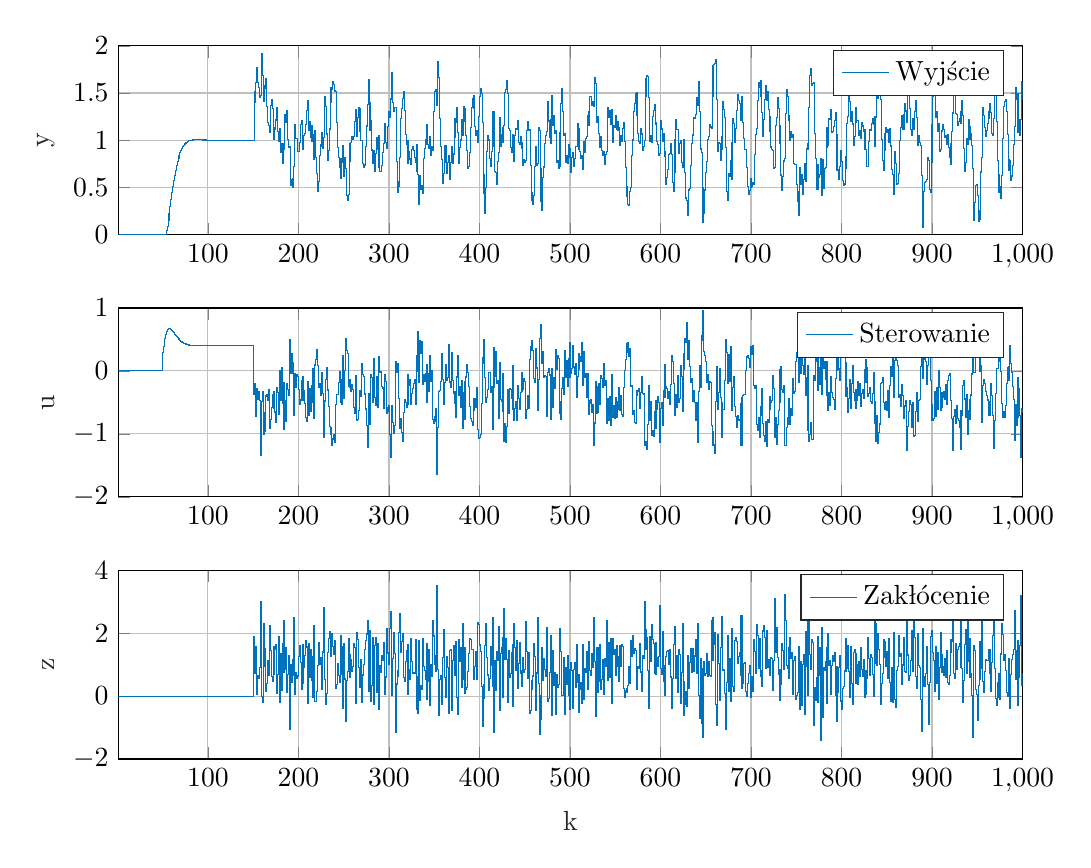
\begin{tikzpicture}

\begin{axis}[%
width=4.521in,
height=0.944in,
at={(0.758in,1.792in)},
scale only axis,
xmin=1,
xmax=1000,
ymin=-2,
ymax=1,
ylabel style={font=\color{white!15!black}},
ylabel={u},
axis background/.style={fill=white},
xmajorgrids,
ymajorgrids,
legend style={legend cell align=left, align=left, draw=white!15!black}
]
\addplot[const plot, color=mycolor1] table[row sep=crcr] {%
1	0\\
2	0\\
3	0\\
4	0\\
5	0\\
6	0\\
7	0\\
8	0\\
9	0\\
10	0\\
11	0\\
12	0\\
13	0\\
14	0\\
15	0\\
16	0\\
17	0\\
18	0\\
19	0\\
20	0\\
21	0\\
22	0\\
23	0\\
24	0\\
25	0\\
26	0\\
27	0\\
28	0\\
29	0\\
30	0\\
31	0\\
32	0\\
33	0\\
34	0\\
35	0\\
36	0\\
37	0\\
38	0\\
39	0\\
40	0\\
41	0\\
42	0\\
43	0\\
44	0\\
45	0\\
46	0\\
47	0\\
48	0\\
49	0\\
50	0.28956\\
51	0.39251\\
52	0.5131\\
53	0.58007\\
54	0.63135\\
55	0.65951\\
56	0.67407\\
57	0.67664\\
58	0.67103\\
59	0.65931\\
60	0.64358\\
61	0.62529\\
62	0.60567\\
63	0.58562\\
64	0.56581\\
65	0.54674\\
66	0.52873\\
67	0.512\\
68	0.49669\\
69	0.48283\\
70	0.47042\\
71	0.45942\\
72	0.44977\\
73	0.44136\\
74	0.4341\\
75	0.42788\\
76	0.4226\\
77	0.41815\\
78	0.41444\\
79	0.41136\\
80	0.40884\\
81	0.4068\\
82	0.40516\\
83	0.40387\\
84	0.40286\\
85	0.40209\\
86	0.40151\\
87	0.4011\\
88	0.40081\\
89	0.40063\\
90	0.40052\\
91	0.40048\\
92	0.40048\\
93	0.40051\\
94	0.40057\\
95	0.40065\\
96	0.40073\\
97	0.40082\\
98	0.40091\\
99	0.401\\
100	0.40108\\
101	0.40116\\
102	0.40123\\
103	0.4013\\
104	0.40136\\
105	0.40142\\
106	0.40146\\
107	0.4015\\
108	0.40154\\
109	0.40157\\
110	0.4016\\
111	0.40162\\
112	0.40164\\
113	0.40166\\
114	0.40167\\
115	0.40168\\
116	0.40169\\
117	0.4017\\
118	0.4017\\
119	0.40171\\
120	0.40171\\
121	0.40171\\
122	0.40171\\
123	0.40172\\
124	0.40172\\
125	0.40172\\
126	0.40172\\
127	0.40172\\
128	0.40172\\
129	0.40172\\
130	0.40172\\
131	0.40172\\
132	0.40172\\
133	0.40171\\
134	0.40171\\
135	0.40171\\
136	0.40171\\
137	0.40171\\
138	0.40171\\
139	0.40171\\
140	0.40171\\
141	0.40171\\
142	0.40171\\
143	0.40171\\
144	0.40171\\
145	0.40171\\
146	0.40171\\
147	0.40171\\
148	0.40171\\
149	0.40171\\
150	-0.3736\\
151	-0.20459\\
152	-0.36541\\
153	-0.7267\\
154	-0.27791\\
155	-0.44758\\
156	-0.32703\\
157	-0.46704\\
158	-1.3402\\
159	-0.47919\\
160	-0.32268\\
161	-1.0057\\
162	-0.66522\\
163	-0.96188\\
164	-0.39777\\
165	-0.37284\\
166	-0.47406\\
167	-0.30291\\
168	-0.92007\\
169	-0.77753\\
170	-0.58179\\
171	-0.37947\\
172	-0.32541\\
173	-0.59809\\
174	-0.65242\\
175	-0.82491\\
176	-0.26789\\
177	-0.34821\\
178	-0.6959\\
179	-0.00024138\\
180	-0.47225\\
181	0.048407\\
182	-0.51177\\
183	-0.18694\\
184	-0.92483\\
185	-0.46771\\
186	-0.80167\\
187	-0.19468\\
188	-0.29531\\
189	-0.38742\\
190	0.49619\\
191	-0.032215\\
192	0.27777\\
193	0.13167\\
194	-0.046907\\
195	-0.71291\\
196	-0.034529\\
197	-0.26214\\
198	-0.057258\\
199	-0.086806\\
200	-0.29179\\
201	-0.52877\\
202	-0.46228\\
203	-0.15293\\
204	-0.091929\\
205	-0.47418\\
206	-0.3085\\
207	-0.51481\\
208	-0.74277\\
209	-0.8092\\
210	-0.17311\\
211	-0.7147\\
212	-0.27447\\
213	-0.63577\\
214	-0.24008\\
215	-0.50679\\
216	0.044381\\
217	-0.75256\\
218	0.094574\\
219	0.17707\\
220	0.3402\\
221	0.092697\\
222	-0.2625\\
223	-0.20363\\
224	-0.38223\\
225	-0.025329\\
226	-0.14677\\
227	-0.36236\\
228	-1.0628\\
229	-0.47774\\
230	-0.13019\\
231	0.053542\\
232	-0.30216\\
233	-0.57019\\
234	-0.87663\\
235	-1.0129\\
236	-0.89303\\
237	-1.1808\\
238	-1.0816\\
239	-1.017\\
240	-1.137\\
241	-0.52666\\
242	-0.3678\\
243	-0.37531\\
244	-0.17853\\
245	-0.015929\\
246	-0.50362\\
247	-0.14114\\
248	-0.53034\\
249	0.24296\\
250	-0.42938\\
251	0.010822\\
252	0.52026\\
253	0.31818\\
254	0.27437\\
255	-0.24507\\
256	-0.26903\\
257	-0.13816\\
258	-0.3288\\
259	-0.21827\\
260	-0.29599\\
261	-0.58669\\
262	-0.67991\\
263	-0.068016\\
264	-0.78072\\
265	-0.77467\\
266	-0.63358\\
267	-0.30961\\
268	-0.35673\\
269	-0.40907\\
270	0.11161\\
271	-0.052885\\
272	-0.09303\\
273	-0.3669\\
274	-0.60535\\
275	-0.87062\\
276	-1.2219\\
277	-0.57785\\
278	-0.36717\\
279	-0.85525\\
280	-0.056084\\
281	-0.10903\\
282	-0.4965\\
283	0.20021\\
284	-0.41732\\
285	-0.54868\\
286	-0.085356\\
287	-0.58153\\
288	0.22368\\
289	0.018877\\
290	-0.016842\\
291	-0.013197\\
292	-0.24097\\
293	-0.27158\\
294	-0.59068\\
295	-0.055445\\
296	-0.16743\\
297	-0.66804\\
298	-0.58961\\
299	-0.64808\\
300	-0.5533\\
301	-1.0088\\
302	-1.3669\\
303	-0.55135\\
304	-0.81697\\
305	-0.98866\\
306	-0.86493\\
307	0.15576\\
308	-0.022453\\
309	0.12457\\
310	0.049704\\
311	-0.4413\\
312	-0.91827\\
313	-0.75367\\
314	-0.98268\\
315	-1.1159\\
316	-0.65993\\
317	-0.4558\\
318	-0.49706\\
319	-0.57967\\
320	-0.058051\\
321	-0.52731\\
322	-0.22275\\
323	-0.12941\\
324	-0.53015\\
325	-0.36324\\
326	-0.2805\\
327	-0.19796\\
328	-0.1334\\
329	-0.52902\\
330	0.24372\\
331	-0.0043916\\
332	0.62045\\
333	-0.17611\\
334	0.47599\\
335	0.28309\\
336	0.45953\\
337	-0.20991\\
338	-0.061345\\
339	-0.16253\\
340	-0.039454\\
341	-0.49274\\
342	0.10209\\
343	-0.04705\\
344	-0.33276\\
345	0.23702\\
346	-0.16826\\
347	0.012145\\
348	-0.77694\\
349	-0.83111\\
350	-0.73097\\
351	-0.80593\\
352	-0.59763\\
353	-1.6513\\
354	-0.89467\\
355	-0.32074\\
356	-0.308\\
357	-0.16359\\
358	0.26932\\
359	-0.13267\\
360	-0.52567\\
361	-0.18881\\
362	0.075119\\
363	0.1023\\
364	-0.15712\\
365	-0.1071\\
366	0.42665\\
367	-0.17638\\
368	-0.25819\\
369	0.29784\\
370	-0.15669\\
371	-0.35677\\
372	-0.52127\\
373	-0.3244\\
374	-0.73186\\
375	-0.097029\\
376	0.24522\\
377	-0.3953\\
378	-0.24868\\
379	-0.58439\\
380	-0.15119\\
381	-0.90686\\
382	-0.34225\\
383	-0.76647\\
384	-0.16176\\
385	-0.096521\\
386	0.093489\\
387	-0.019289\\
388	-0.24791\\
389	-0.56541\\
390	-0.75858\\
391	-0.80188\\
392	-0.87004\\
393	-0.62538\\
394	-0.43118\\
395	-0.44116\\
396	-0.58431\\
397	-0.2715\\
398	-0.93576\\
399	-1.0665\\
400	-1.0643\\
401	-1.0104\\
402	-0.52196\\
403	0.20927\\
404	0.12045\\
405	0.49156\\
406	-0.099425\\
407	-0.50838\\
408	-0.42764\\
409	-0.29526\\
410	-0.019603\\
411	-0.02085\\
412	-0.34703\\
413	-0.24155\\
414	-0.93217\\
415	-0.26975\\
416	0.37652\\
417	-0.086573\\
418	0.31326\\
419	-0.1938\\
420	-0.14906\\
421	-0.74847\\
422	0.13169\\
423	-0.46012\\
424	-0.49252\\
425	-0.039398\\
426	-0.64298\\
427	-1.1171\\
428	-0.83142\\
429	-1.1357\\
430	-0.87663\\
431	-0.30044\\
432	-0.66778\\
433	-0.27285\\
434	-0.28998\\
435	-0.44154\\
436	-0.60915\\
437	0.077648\\
438	-0.78063\\
439	-0.5978\\
440	-0.49296\\
441	-0.78454\\
442	-0.23172\\
443	-0.43749\\
444	-0.61293\\
445	-0.34279\\
446	-0.32804\\
447	-0.028848\\
448	-0.29144\\
449	-0.11412\\
450	-0.16407\\
451	-0.75709\\
452	-0.61272\\
453	-0.39187\\
454	-0.59583\\
455	0.18539\\
456	0.38998\\
457	0.32404\\
458	0.47577\\
459	0.32442\\
460	-0.12471\\
461	-0.19015\\
462	0.34796\\
463	0.046059\\
464	-0.625\\
465	-0.13176\\
466	0.51771\\
467	0.73648\\
468	0.7099\\
469	0.12267\\
470	0.30402\\
471	-0.1001\\
472	-0.066179\\
473	-0.091408\\
474	-0.72594\\
475	-0.019147\\
476	0.031058\\
477	-0.06417\\
478	-0.49298\\
479	-0.76428\\
480	0.034818\\
481	-0.57611\\
482	-0.10616\\
483	-0.28397\\
484	0.3432\\
485	0.021044\\
486	0.2521\\
487	0.19851\\
488	-0.48257\\
489	-0.67752\\
490	-0.76445\\
491	-0.27865\\
492	-0.098201\\
493	-0.37074\\
494	0.31894\\
495	-0.10741\\
496	0.16099\\
497	-0.24575\\
498	0.19396\\
499	-0.099431\\
500	0.45141\\
501	-0.039247\\
502	0.037071\\
503	0.4026\\
504	0.062356\\
505	-0.058607\\
506	0.10939\\
507	-0.42319\\
508	-0.088942\\
509	0.26835\\
510	0.024253\\
511	0.23568\\
512	0.15351\\
513	0.45091\\
514	-0.22978\\
515	0.31153\\
516	-0.1005\\
517	-0.039647\\
518	-0.41828\\
519	-0.048071\\
520	-0.4734\\
521	-0.6855\\
522	-0.52416\\
523	-0.45626\\
524	-0.65894\\
525	-0.52853\\
526	-1.19\\
527	-0.82647\\
528	-0.16179\\
529	-0.67834\\
530	-0.66121\\
531	-0.24032\\
532	-0.20388\\
533	-0.53526\\
534	-0.066368\\
535	-0.12122\\
536	-0.25683\\
537	0.1251\\
538	-0.22951\\
539	-0.15689\\
540	-0.8346\\
541	-0.65003\\
542	-0.44114\\
543	-0.78634\\
544	-0.40021\\
545	-0.86217\\
546	-0.064485\\
547	-0.74218\\
548	-0.54861\\
549	-0.75027\\
550	-0.42745\\
551	-0.74077\\
552	-0.4916\\
553	-0.61933\\
554	-0.26637\\
555	-0.63054\\
556	-0.39141\\
557	-0.69423\\
558	-0.71802\\
559	-0.26831\\
560	0.011178\\
561	0.17757\\
562	0.29836\\
563	0.44072\\
564	0.44327\\
565	0.22589\\
566	0.348\\
567	-0.23979\\
568	-0.23113\\
569	-0.6841\\
570	-0.631\\
571	-0.81531\\
572	-0.84\\
573	-0.3963\\
574	-0.30557\\
575	-0.3284\\
576	-0.28071\\
577	-0.59979\\
578	-0.34017\\
579	-0.08599\\
580	-0.36281\\
581	-0.36589\\
582	-1.1868\\
583	-1.1513\\
584	-1.1267\\
585	-1.2517\\
586	-0.8493\\
587	-0.22525\\
588	-0.78612\\
589	-0.48464\\
590	-1.0262\\
591	-0.94898\\
592	-1.0347\\
593	-0.6459\\
594	-0.91556\\
595	-0.47725\\
596	-0.60599\\
597	-0.40699\\
598	-0.49867\\
599	-1.1365\\
600	-0.60264\\
601	-0.50684\\
602	-0.85936\\
603	-0.31647\\
604	-0.42296\\
605	0.099671\\
606	-0.24228\\
607	-0.28221\\
608	-0.43192\\
609	-0.31965\\
610	-0.5274\\
611	-0.21415\\
612	0.24811\\
613	0.14351\\
614	-0.20519\\
615	-0.61596\\
616	-0.70225\\
617	-0.38123\\
618	-0.57514\\
619	-0.076197\\
620	-0.49449\\
621	-0.44118\\
622	0.080942\\
623	-0.093769\\
624	-0.64004\\
625	0.27757\\
626	0.024042\\
627	0.51232\\
628	0.44543\\
629	0.76226\\
630	0.19013\\
631	0.48063\\
632	0.064358\\
633	-0.18931\\
634	-0.11447\\
635	-0.47695\\
636	-0.31944\\
637	-0.34391\\
638	-0.5059\\
639	-0.78352\\
640	-0.50592\\
641	-1.1301\\
642	-0.33233\\
643	0.08204\\
644	-0.26634\\
645	0.56039\\
646	0.96155\\
647	0.47713\\
648	0.30704\\
649	0.24777\\
650	0.14357\\
651	-0.18906\\
652	-0.051069\\
653	-0.29784\\
654	-0.17358\\
655	-0.17937\\
656	-0.87335\\
657	-1.1893\\
658	-0.96842\\
659	-1.1693\\
660	-1.3149\\
661	-0.49128\\
662	0.075445\\
663	-0.61547\\
664	-0.33691\\
665	0.04001\\
666	-0.42149\\
667	-0.50095\\
668	-1.0616\\
669	-0.61382\\
670	-0.61105\\
671	-0.15598\\
672	0.50184\\
673	0.28883\\
674	-0.20222\\
675	0.253\\
676	-0.15971\\
677	0.37958\\
678	-0.50566\\
679	-0.63279\\
680	-0.2634\\
681	-0.088792\\
682	-0.56372\\
683	-0.72879\\
684	-0.89328\\
685	-0.71344\\
686	-0.78031\\
687	-0.79329\\
688	-0.51889\\
689	-1.1913\\
690	-0.41758\\
691	-0.38336\\
692	-0.37142\\
693	-0.37427\\
694	0.0091025\\
695	0.22162\\
696	0.24395\\
697	0.19168\\
698	0.055071\\
699	0.3949\\
700	0.28412\\
701	0.26422\\
702	0.40645\\
703	-0.22753\\
704	-0.28262\\
705	-0.22488\\
706	-0.85244\\
707	-0.93952\\
708	-0.7407\\
709	-1.0611\\
710	-0.70591\\
711	-0.57353\\
712	-0.27771\\
713	-0.8324\\
714	-1.025\\
715	-1.1187\\
716	-0.81104\\
717	-1.1975\\
718	-0.76736\\
719	-0.81646\\
720	-0.61265\\
721	-0.412\\
722	-0.50111\\
723	-0.4674\\
724	-0.06578\\
725	-0.28179\\
726	-1.0608\\
727	-0.73771\\
728	-1.173\\
729	-0.84973\\
730	-0.63287\\
731	-0.49679\\
732	0.026223\\
733	0.062967\\
734	-0.29166\\
735	-0.3427\\
736	-0.23643\\
737	-1.1809\\
738	-1.1901\\
739	-0.90272\\
740	-0.74523\\
741	-0.84983\\
742	-0.44301\\
743	-0.84391\\
744	-0.59461\\
745	-0.70692\\
746	-0.1163\\
747	-0.3611\\
748	-0.33102\\
749	0.15345\\
750	0.29992\\
751	0.47248\\
752	-0.031577\\
753	-0.18338\\
754	0.40841\\
755	-0.036906\\
756	0.54086\\
757	0.079894\\
758	-0.050839\\
759	0.51987\\
760	-0.38274\\
761	-0.10555\\
762	0.087217\\
763	-0.94255\\
764	-1.1194\\
765	-1.0078\\
766	-0.81633\\
767	-1.0839\\
768	-1.0833\\
769	-0.072523\\
770	-0.1588\\
771	0.30263\\
772	0.14874\\
773	-0.30734\\
774	0.31103\\
775	0.058757\\
776	-0.21641\\
777	0.79557\\
778	-0.37073\\
779	0.65865\\
780	0.037468\\
781	0.1536\\
782	-0.12818\\
783	-0.38532\\
784	0.15642\\
785	-0.62202\\
786	-0.34276\\
787	-0.54695\\
788	-0.085452\\
789	-0.33793\\
790	-0.41911\\
791	-0.45225\\
792	-0.60847\\
793	-0.11916\\
794	0.36646\\
795	0.0053025\\
796	0.34662\\
797	0.030306\\
798	-0.14709\\
799	0.27071\\
800	0.4908\\
801	0.43571\\
802	0.44585\\
803	0.2112\\
804	0.13391\\
805	-0.40351\\
806	-0.25967\\
807	-0.66148\\
808	-0.4395\\
809	-0.13054\\
810	-0.59221\\
811	-0.20015\\
812	0.091202\\
813	-0.3427\\
814	-0.46174\\
815	-0.60098\\
816	-0.29364\\
817	-0.4631\\
818	-0.16325\\
819	-0.39192\\
820	-0.19828\\
821	-0.56869\\
822	-0.36198\\
823	-0.30193\\
824	-0.43361\\
825	0.024116\\
826	-0.18687\\
827	0.18794\\
828	0.055305\\
829	-0.41236\\
830	-0.36448\\
831	-0.27175\\
832	-0.49182\\
833	-0.51373\\
834	-0.36143\\
835	-0.023578\\
836	-0.84224\\
837	-0.4863\\
838	-1.1265\\
839	-0.70401\\
840	-1.1535\\
841	-0.97719\\
842	-0.84392\\
843	-0.20268\\
844	-0.18387\\
845	-0.10007\\
846	-0.50317\\
847	-0.61715\\
848	-0.58266\\
849	-0.48786\\
850	-0.63081\\
851	-0.30839\\
852	-0.74091\\
853	-0.23445\\
854	0.076597\\
855	-0.082733\\
856	0.39552\\
857	-0.065439\\
858	-0.41364\\
859	0.16666\\
860	0.37585\\
861	0.16669\\
862	0.089395\\
863	-0.42579\\
864	-0.38139\\
865	-0.56269\\
866	-0.22185\\
867	-0.39068\\
868	-0.70007\\
869	-0.75556\\
870	-0.55646\\
871	-0.46937\\
872	-1.26\\
873	-0.87773\\
874	-0.64029\\
875	-0.47738\\
876	-0.53035\\
877	-0.89017\\
878	-0.50941\\
879	-0.61391\\
880	-1.0352\\
881	-1.0299\\
882	-0.6468\\
883	-0.33704\\
884	-0.80068\\
885	-0.47105\\
886	-0.45954\\
887	0.06453\\
888	0.69305\\
889	0.51902\\
890	-0.11935\\
891	0.18537\\
892	0.21254\\
893	0.14933\\
894	-0.22057\\
895	0.091202\\
896	0.62205\\
897	0.38196\\
898	-0.15701\\
899	-0.52853\\
900	-0.79096\\
901	-0.7828\\
902	-0.76012\\
903	-0.33049\\
904	-0.72885\\
905	-0.26111\\
906	-0.60601\\
907	0.013662\\
908	-0.26004\\
909	-0.62323\\
910	-0.34257\\
911	-0.58011\\
912	-0.42641\\
913	-0.32321\\
914	-0.45317\\
915	-0.22284\\
916	-0.52535\\
917	-0.15417\\
918	-0.068952\\
919	-0.041106\\
920	-0.46838\\
921	-0.47202\\
922	-0.74906\\
923	-1.2703\\
924	-0.7279\\
925	-0.60725\\
926	-0.8385\\
927	-0.54727\\
928	-0.75555\\
929	-0.78987\\
930	-0.89651\\
931	-0.63279\\
932	-1.2397\\
933	-0.70454\\
934	-0.2313\\
935	-0.15669\\
936	-0.44575\\
937	-0.74275\\
938	-0.37812\\
939	-1.0117\\
940	-0.62498\\
941	-0.451\\
942	-0.76429\\
943	-0.38301\\
944	-0.049254\\
945	0.75888\\
946	-0.018036\\
947	-0.017819\\
948	0.2251\\
949	0.38424\\
950	0.85355\\
951	0.62228\\
952	0.58012\\
953	-0.014324\\
954	0.07886\\
955	-0.81834\\
956	-0.23684\\
957	-0.14251\\
958	-0.19587\\
959	-0.33093\\
960	-0.39478\\
961	-0.46212\\
962	-0.59228\\
963	-0.70984\\
964	-0.49371\\
965	-0.1955\\
966	-0.38795\\
967	-0.71178\\
968	-1.2367\\
969	-0.78384\\
970	-0.36179\\
971	0.041078\\
972	0.037715\\
973	0.3528\\
974	0.15497\\
975	0.50651\\
976	-0.01326\\
977	-0.51338\\
978	-0.74303\\
979	-0.64316\\
980	-0.74672\\
981	-0.54714\\
982	-0.20593\\
983	0.045826\\
984	0.062163\\
985	-0.15447\\
986	0.40636\\
987	0.11255\\
988	-0.022775\\
989	-0.24788\\
990	-0.45021\\
991	-1.1047\\
992	-0.52815\\
993	-0.87314\\
994	-0.10634\\
995	-0.7439\\
996	-0.27294\\
997	-0.70937\\
998	-1.3793\\
999	-0.60388\\
1000	-0.66098\\
};
\addlegendentry{Sterowanie}

\end{axis}

\begin{axis}[%
width=4.521in,
height=0.944in,
at={(0.758in,3.103in)},
scale only axis,
xmin=1,
xmax=1000,
ymin=0,
ymax=2,
ylabel style={font=\color{white!15!black}},
ylabel={y},
axis background/.style={fill=white},
xmajorgrids,
ymajorgrids,
legend style={legend cell align=left, align=left, draw=white!15!black}
]
\addplot[const plot, color=mycolor1] table[row sep=crcr] {%
1	0\\
2	0\\
3	0\\
4	0\\
5	0\\
6	0\\
7	0\\
8	0\\
9	0\\
10	0\\
11	0\\
12	0\\
13	0\\
14	0\\
15	0\\
16	0\\
17	0\\
18	0\\
19	0\\
20	0\\
21	0\\
22	0\\
23	0\\
24	0\\
25	0\\
26	0\\
27	0\\
28	0\\
29	0\\
30	0\\
31	0\\
32	0\\
33	0\\
34	0\\
35	0\\
36	0\\
37	0\\
38	0\\
39	0\\
40	0\\
41	0\\
42	0\\
43	0\\
44	0\\
45	0\\
46	0\\
47	0\\
48	0\\
49	0\\
50	0\\
51	0\\
52	0\\
53	0\\
54	0.039119\\
55	0.090032\\
56	0.15448\\
57	0.22449\\
58	0.29764\\
59	0.37063\\
60	0.44164\\
61	0.50914\\
62	0.57223\\
63	0.63032\\
64	0.68313\\
65	0.73061\\
66	0.77286\\
67	0.81011\\
68	0.84266\\
69	0.87086\\
70	0.8951\\
71	0.91576\\
72	0.93322\\
73	0.94786\\
74	0.96003\\
75	0.97004\\
76	0.97821\\
77	0.98479\\
78	0.99003\\
79	0.99414\\
80	0.99731\\
81	0.99971\\
82	1.0015\\
83	1.0027\\
84	1.0036\\
85	1.0041\\
86	1.0043\\
87	1.0044\\
88	1.0043\\
89	1.0042\\
90	1.0039\\
91	1.0036\\
92	1.0033\\
93	1.003\\
94	1.0027\\
95	1.0024\\
96	1.0021\\
97	1.0018\\
98	1.0016\\
99	1.0013\\
100	1.0011\\
101	1.001\\
102	1.0008\\
103	1.0007\\
104	1.0005\\
105	1.0004\\
106	1.0003\\
107	1.0003\\
108	1.0002\\
109	1.0002\\
110	1.0001\\
111	1.0001\\
112	1.0001\\
113	1\\
114	1\\
115	1\\
116	1\\
117	0.99999\\
118	0.99998\\
119	0.99998\\
120	0.99998\\
121	0.99998\\
122	0.99998\\
123	0.99998\\
124	0.99998\\
125	0.99998\\
126	0.99998\\
127	0.99998\\
128	0.99998\\
129	0.99998\\
130	0.99998\\
131	0.99998\\
132	0.99999\\
133	0.99999\\
134	0.99999\\
135	0.99999\\
136	0.99999\\
137	0.99999\\
138	0.99999\\
139	0.99999\\
140	0.99999\\
141	0.99999\\
142	0.99999\\
143	0.99999\\
144	0.99999\\
145	0.99999\\
146	0.99999\\
147	0.99999\\
148	0.99999\\
149	0.99999\\
150	0.99999\\
151	1.4031\\
152	1.5144\\
153	1.6069\\
154	1.7723\\
155	1.6071\\
156	1.5615\\
157	1.4491\\
158	1.4758\\
159	1.922\\
160	1.6838\\
161	1.4084\\
162	1.5775\\
163	1.5441\\
164	1.6479\\
165	1.3529\\
166	1.1882\\
167	1.1516\\
168	1.0842\\
169	1.3665\\
170	1.4306\\
171	1.3369\\
172	1.1325\\
173	1.013\\
174	1.1165\\
175	1.2146\\
176	1.3428\\
177	1.088\\
178	0.9824\\
179	1.12\\
180	0.86666\\
181	0.96327\\
182	0.7489\\
183	0.96876\\
184	0.90391\\
185	1.2726\\
186	1.1921\\
187	1.3106\\
188	1.0112\\
189	0.9262\\
190	0.93278\\
191	0.52109\\
192	0.5836\\
193	0.49989\\
194	0.59255\\
195	0.72076\\
196	1.1606\\
197	1.0151\\
198	1.0139\\
199	0.88423\\
200	0.87608\\
201	0.97354\\
202	1.1628\\
203	1.2112\\
204	1.043\\
205	0.90591\\
206	1.0535\\
207	1.0692\\
208	1.1707\\
209	1.3153\\
210	1.4193\\
211	1.1044\\
212	1.1968\\
213	1.0325\\
214	1.1582\\
215	0.99177\\
216	1.0614\\
217	0.7995\\
218	1.1014\\
219	0.82041\\
220	0.64345\\
221	0.45317\\
222	0.56714\\
223	0.83925\\
224	0.95885\\
225	1.0818\\
226	0.93351\\
227	0.91699\\
228	1.0243\\
229	1.4656\\
230	1.3599\\
231	1.0654\\
232	0.7843\\
233	0.88719\\
234	1.1187\\
235	1.3949\\
236	1.5602\\
237	1.5333\\
238	1.6225\\
239	1.5927\\
240	1.5215\\
241	1.5126\\
242	1.1852\\
243	0.92505\\
244	0.81263\\
245	0.71145\\
246	0.59603\\
247	0.81085\\
248	0.76429\\
249	0.94192\\
250	0.6142\\
251	0.81471\\
252	0.70103\\
253	0.41578\\
254	0.35746\\
255	0.42503\\
256	0.77889\\
257	0.96711\\
258	0.97289\\
259	1.0346\\
260	1.0111\\
261	1.0397\\
262	1.194\\
263	1.3218\\
264	1.0416\\
265	1.2368\\
266	1.3474\\
267	1.3367\\
268	1.098\\
269	1.0001\\
270	1.0005\\
271	0.75271\\
272	0.71042\\
273	0.73696\\
274	0.93447\\
275	1.1506\\
276	1.3826\\
277	1.644\\
278	1.3963\\
279	1.1084\\
280	1.208\\
281	0.89626\\
282	0.75878\\
283	0.89343\\
284	0.66423\\
285	0.85557\\
286	1.03\\
287	0.90645\\
288	1.0502\\
289	0.71533\\
290	0.66856\\
291	0.67003\\
292	0.73164\\
293	0.8741\\
294	0.96621\\
295	1.1718\\
296	0.97715\\
297	0.91716\\
298	1.1467\\
299	1.2574\\
300	1.3076\\
301	1.24\\
302	1.4366\\
303	1.7117\\
304	1.3973\\
305	1.3075\\
306	1.3476\\
307	1.3441\\
308	0.77397\\
309	0.56695\\
310	0.44934\\
311	0.51479\\
312	0.81394\\
313	1.2338\\
314	1.3353\\
315	1.4393\\
316	1.5198\\
317	1.3108\\
318	1.0617\\
319	0.95971\\
320	0.99394\\
321	0.75529\\
322	0.87554\\
323	0.80102\\
324	0.73956\\
325	0.90183\\
326	0.93078\\
327	0.89529\\
328	0.81383\\
329	0.75939\\
330	0.95386\\
331	0.66477\\
332	0.64023\\
333	0.31677\\
334	0.63027\\
335	0.47574\\
336	0.52437\\
337	0.44043\\
338	0.80251\\
339	0.9142\\
340	1.012\\
341	0.95348\\
342	1.1655\\
343	0.95885\\
344	0.91792\\
345	1.0378\\
346	0.84122\\
347	0.92956\\
348	0.88661\\
349	1.3032\\
350	1.5174\\
351	1.5408\\
352	1.5121\\
353	1.3719\\
354	1.8382\\
355	1.6666\\
356	1.2276\\
357	0.93576\\
358	0.79162\\
359	0.54259\\
360	0.64367\\
361	0.94314\\
362	0.94388\\
363	0.76223\\
364	0.64501\\
365	0.76652\\
366	0.8333\\
367	0.58735\\
368	0.76712\\
369	0.93804\\
370	0.75525\\
371	0.85376\\
372	1.0313\\
373	1.2314\\
374	1.1834\\
375	1.3413\\
376	1.0787\\
377	0.75715\\
378	0.92483\\
379	1.0018\\
380	1.2155\\
381	1.0536\\
382	1.3561\\
383	1.2033\\
384	1.3373\\
385	1.0496\\
386	0.88729\\
387	0.70077\\
388	0.71979\\
389	0.87125\\
390	1.1301\\
391	1.3445\\
392	1.4378\\
393	1.4758\\
394	1.3367\\
395	1.1455\\
396	1.051\\
397	1.1013\\
398	0.97674\\
399	1.2511\\
400	1.4585\\
401	1.5476\\
402	1.4935\\
403	1.1857\\
404	0.64065\\
405	0.43732\\
406	0.22471\\
407	0.49774\\
408	0.88029\\
409	1.0468\\
410	1.002\\
411	0.80715\\
412	0.72283\\
413	0.87848\\
414	0.93006\\
415	1.3043\\
416	1.1264\\
417	0.67077\\
418	0.65795\\
419	0.53174\\
420	0.77317\\
421	0.8662\\
422	1.2393\\
423	0.93341\\
424	1.0594\\
425	1.1322\\
426	0.97143\\
427	1.1551\\
428	1.5098\\
429	1.5397\\
430	1.6301\\
431	1.4988\\
432	1.1227\\
433	1.1001\\
434	0.92445\\
435	0.87209\\
436	0.91741\\
437	1.0609\\
438	0.77037\\
439	1.053\\
440	1.122\\
441	1.1155\\
442	1.2032\\
443	0.97373\\
444	0.95654\\
445	1.0419\\
446	0.97838\\
447	0.91528\\
448	0.72771\\
449	0.79558\\
450	0.75982\\
451	0.78631\\
452	1.1032\\
453	1.2028\\
454	1.1045\\
455	1.1165\\
456	0.73283\\
457	0.44106\\
458	0.35773\\
459	0.32358\\
460	0.41885\\
461	0.72251\\
462	0.92976\\
463	0.72989\\
464	0.75254\\
465	1.1382\\
466	1.1071\\
467	0.69722\\
468	0.34672\\
469	0.26127\\
470	0.60333\\
471	0.7167\\
472	0.96771\\
473	1.0454\\
474	1.093\\
475	1.4147\\
476	1.2034\\
477	1.0295\\
478	0.96785\\
479	1.2144\\
480	1.4777\\
481	1.1597\\
482	1.2605\\
483	1.0741\\
484	1.1005\\
485	0.75917\\
486	0.78299\\
487	0.69606\\
488	0.722\\
489	1.0845\\
490	1.3892\\
491	1.5489\\
492	1.3026\\
493	1.0507\\
494	1.0722\\
495	0.76732\\
496	0.83853\\
497	0.75092\\
498	0.95867\\
499	0.82028\\
500	0.90883\\
501	0.66\\
502	0.81579\\
503	0.8653\\
504	0.72623\\
505	0.80471\\
506	0.93618\\
507	0.93286\\
508	1.1789\\
509	1.1263\\
510	0.89822\\
511	0.88191\\
512	0.80734\\
513	0.83347\\
514	0.68835\\
515	0.98815\\
516	0.87107\\
517	1.0209\\
518	1.0387\\
519	1.2665\\
520	1.1563\\
521	1.3024\\
522	1.4667\\
523	1.4638\\
524	1.3707\\
525	1.406\\
526	1.359\\
527	1.6635\\
528	1.6042\\
529	1.1903\\
530	1.2011\\
531	1.2482\\
532	1.0757\\
533	0.92639\\
534	1.0428\\
535	0.89348\\
536	0.83655\\
537	0.87821\\
538	0.7394\\
539	0.84991\\
540	0.88171\\
541	1.2688\\
542	1.3444\\
543	1.2411\\
544	1.315\\
545	1.1659\\
546	1.3236\\
547	0.97218\\
548	1.1504\\
549	1.1383\\
550	1.2643\\
551	1.1119\\
552	1.1974\\
553	1.1056\\
554	1.1319\\
555	0.94549\\
556	1.0525\\
557	0.98875\\
558	1.1248\\
559	1.1879\\
560	0.98683\\
561	0.7126\\
562	0.5088\\
563	0.40098\\
564	0.31828\\
565	0.31349\\
566	0.4614\\
567	0.50377\\
568	0.83806\\
569	1.0026\\
570	1.3078\\
571	1.3856\\
572	1.49\\
573	1.509\\
574	1.2671\\
575	1.0685\\
576	0.99052\\
577	0.96248\\
578	1.121\\
579	1.0661\\
580	0.89318\\
581	0.93665\\
582	0.99383\\
583	1.4586\\
584	1.6491\\
585	1.6804\\
586	1.6793\\
587	1.4515\\
588	0.98954\\
589	1.0469\\
590	0.97686\\
591	1.2468\\
592	1.3124\\
593	1.3819\\
594	1.1672\\
595	1.1919\\
596	0.98182\\
597	0.9576\\
598	0.84204\\
599	0.86254\\
600	1.209\\
601	1.1189\\
602	0.9842\\
603	1.072\\
604	0.87846\\
605	0.8286\\
606	0.53306\\
607	0.60725\\
608	0.69436\\
609	0.85304\\
610	0.85538\\
611	0.95961\\
612	0.84598\\
613	0.55\\
614	0.46035\\
615	0.6549\\
616	1.0121\\
617	1.2213\\
618	1.1127\\
619	1.117\\
620	0.86245\\
621	0.96577\\
622	0.99975\\
623	0.76571\\
624	0.71128\\
625	1.0019\\
626	0.70949\\
627	0.65997\\
628	0.38838\\
629	0.3581\\
630	0.19946\\
631	0.47278\\
632	0.49037\\
633	0.73109\\
634	0.96624\\
635	1.0549\\
636	1.2445\\
637	1.237\\
638	1.227\\
639	1.2767\\
640	1.4482\\
641	1.3703\\
642	1.6172\\
643	1.303\\
644	0.90664\\
645	0.86917\\
646	0.50221\\
647	0.13371\\
648	0.22906\\
649	0.47258\\
650	0.65852\\
651	0.77744\\
652	1.0041\\
653	1.0416\\
654	1.1653\\
655	1.1402\\
656	1.1245\\
657	1.4589\\
658	1.7929\\
659	1.7978\\
660	1.8127\\
661	1.8553\\
662	1.4303\\
663	0.87722\\
664	0.9744\\
665	0.96929\\
666	0.78651\\
667	0.89804\\
668	1.0395\\
669	1.4139\\
670	1.3272\\
671	1.2401\\
672	0.92702\\
673	0.45711\\
674	0.35844\\
675	0.64579\\
676	0.6132\\
677	0.78649\\
678	0.58644\\
679	0.97134\\
680	1.2324\\
681	1.1728\\
682	0.97212\\
683	1.1198\\
684	1.3144\\
685	1.485\\
686	1.4224\\
687	1.3908\\
688	1.3635\\
689	1.2057\\
690	1.4604\\
691	1.1886\\
692	1.0144\\
693	0.8989\\
694	0.9036\\
695	0.71391\\
696	0.51438\\
697	0.43022\\
698	0.4701\\
699	0.59665\\
700	0.49917\\
701	0.51165\\
702	0.54804\\
703	0.52821\\
704	0.85268\\
705	1.0605\\
706	1.1206\\
707	1.4231\\
708	1.6111\\
709	1.5635\\
710	1.6349\\
711	1.4685\\
712	1.2981\\
713	1.0361\\
714	1.2183\\
715	1.4306\\
716	1.5766\\
717	1.4254\\
718	1.515\\
719	1.3287\\
720	1.2532\\
721	1.0896\\
722	0.92787\\
723	0.89765\\
724	0.89272\\
725	0.69731\\
726	0.71224\\
727	1.1549\\
728	1.2367\\
729	1.4494\\
730	1.3338\\
731	1.1554\\
732	0.96694\\
733	0.63102\\
734	0.46989\\
735	0.61987\\
736	0.77935\\
737	0.80322\\
738	1.2843\\
739	1.5335\\
740	1.4655\\
741	1.2606\\
742	1.21\\
743	0.9935\\
744	1.096\\
745	1.0271\\
746	1.0625\\
747	0.7528\\
748	0.7395\\
749	0.74239\\
750	0.53495\\
751	0.3477\\
752	0.20351\\
753	0.45827\\
754	0.70704\\
755	0.5308\\
756	0.63928\\
757	0.42029\\
758	0.58809\\
759	0.74756\\
760	0.56571\\
761	0.91159\\
762	0.9654\\
763	0.8979\\
764	1.3433\\
765	1.6863\\
766	1.7562\\
767	1.5825\\
768	1.6018\\
769	1.6084\\
770	1.0697\\
771	0.80892\\
772	0.48164\\
773	0.47975\\
774	0.74679\\
775	0.60301\\
776	0.64061\\
777	0.80698\\
778	0.41046\\
779	0.79616\\
780	0.49244\\
781	0.69824\\
782	0.71103\\
783	0.92411\\
784	1.1296\\
785	0.94768\\
786	1.2251\\
787	1.2213\\
788	1.3254\\
789	1.0821\\
790	1.0944\\
791	1.144\\
792	1.2067\\
793	1.2917\\
794	1.065\\
795	0.68191\\
796	0.68755\\
797	0.58115\\
798	0.72484\\
799	0.88904\\
800	0.77408\\
801	0.57475\\
802	0.51622\\
803	0.53637\\
804	0.69789\\
805	0.82858\\
806	1.1723\\
807	1.251\\
808	1.4634\\
809	1.4094\\
810	1.2\\
811	1.3019\\
812	1.1716\\
813	0.94961\\
814	1.0419\\
815	1.1933\\
816	1.343\\
817	1.2133\\
818	1.2115\\
819	1.0507\\
820	1.0997\\
821	1.022\\
822	1.1865\\
823	1.1511\\
824	1.0956\\
825	1.1131\\
826	0.89922\\
827	0.89906\\
828	0.71742\\
829	0.726\\
830	0.983\\
831	1.1169\\
832	1.1056\\
833	1.1773\\
834	1.2281\\
835	1.1659\\
836	0.93467\\
837	1.2456\\
838	1.2425\\
839	1.5568\\
840	1.4381\\
841	1.595\\
842	1.5366\\
843	1.4326\\
844	1.0047\\
845	0.7895\\
846	0.678\\
847	0.88983\\
848	1.0703\\
849	1.1351\\
850	1.0809\\
851	1.1173\\
852	0.97205\\
853	1.1229\\
854	0.9384\\
855	0.6879\\
856	0.63828\\
857	0.4271\\
858	0.59126\\
859	0.88046\\
860	0.75128\\
861	0.53259\\
862	0.5392\\
863	0.65004\\
864	0.99396\\
865	1.1323\\
866	1.2664\\
867	1.1131\\
868	1.1113\\
869	1.2677\\
870	1.3883\\
871	1.3094\\
872	1.1866\\
873	1.5311\\
874	1.5154\\
875	1.3401\\
876	1.109\\
877	1.0508\\
878	1.2313\\
879	1.1317\\
880	1.1108\\
881	1.305\\
882	1.4196\\
883	1.2421\\
884	0.94878\\
885	1.0545\\
886	0.98008\\
887	0.94013\\
888	0.62836\\
889	0.17555\\
890	0.078218\\
891	0.45567\\
892	0.554\\
893	0.56562\\
894	0.58278\\
895	0.82096\\
896	0.78848\\
897	0.48064\\
898	0.44442\\
899	0.76864\\
900	1.1689\\
901	1.4682\\
902	1.5485\\
903	1.5206\\
904	1.245\\
905	1.3\\
906	1.0957\\
907	1.1798\\
908	0.88608\\
909	0.8983\\
910	1.0975\\
911	1.0888\\
912	1.1689\\
913	1.1103\\
914	1.0335\\
915	1.0483\\
916	0.95109\\
917	1.0613\\
918	0.92465\\
919	0.81561\\
920	0.74288\\
921	0.96696\\
922	1.0957\\
923	1.2884\\
924	1.6189\\
925	1.4786\\
926	1.2833\\
927	1.2753\\
928	1.1573\\
929	1.1982\\
930	1.2268\\
931	1.3038\\
932	1.1809\\
933	1.4195\\
934	1.2572\\
935	0.9122\\
936	0.67241\\
937	0.76857\\
938	1.0211\\
939	0.95788\\
940	1.2214\\
941	1.1453\\
942	1.011\\
943	1.0716\\
944	0.93991\\
945	0.69919\\
946	0.15495\\
947	0.34312\\
948	0.52332\\
949	0.53543\\
950	0.41514\\
951	0.13642\\
952	0.16227\\
953	0.25605\\
954	0.66313\\
955	0.81926\\
956	1.3436\\
957	1.2633\\
958	1.1304\\
959	1.0393\\
960	1.1068\\
961	1.176\\
962	1.2311\\
963	1.3067\\
964	1.3894\\
965	1.2969\\
966	1.0684\\
967	1.0462\\
968	1.2306\\
969	1.6078\\
970	1.5231\\
971	1.1956\\
972	0.78728\\
973	0.63376\\
974	0.4509\\
975	0.50646\\
976	0.38276\\
977	0.62363\\
978	1.0228\\
979	1.3557\\
980	1.4065\\
981	1.4256\\
982	1.3044\\
983	1.0561\\
984	0.7933\\
985	0.68292\\
986	0.78455\\
987	0.57349\\
988	0.62115\\
989	0.73639\\
990	0.95236\\
991	1.1446\\
992	1.561\\
993	1.4361\\
994	1.4918\\
995	1.0812\\
996	1.2227\\
997	1.0519\\
998	1.2183\\
999	1.6196\\
1000	1.4249\\
};
\addlegendentry{Wyjście}

\end{axis}

\begin{axis}[%
width=4.521in,
height=0.944in,
at={(0.758in,0.481in)},
scale only axis,
xmin=1,
xmax=1000,
xlabel style={font=\color{white!15!black}},
xlabel={k},
ymin=-2,
ymax=4,
ylabel style={font=\color{white!15!black}},
ylabel={z},
axis background/.style={fill=white},
xmajorgrids,
ymajorgrids,
legend style={legend cell align=left, align=left, draw=white!15!black}
]
\addplot[const plot, color=mycolor1] table[row sep=crcr] {%
1	0\\
2	0\\
3	0\\
4	0\\
5	0\\
6	0\\
7	0\\
8	0\\
9	0\\
10	0\\
11	0\\
12	0\\
13	0\\
14	0\\
15	0\\
16	0\\
17	0\\
18	0\\
19	0\\
20	0\\
21	0\\
22	0\\
23	0\\
24	0\\
25	0\\
26	0\\
27	0\\
28	0\\
29	0\\
30	0\\
31	0\\
32	0\\
33	0\\
34	0\\
35	0\\
36	0\\
37	0\\
38	0\\
39	0\\
40	0\\
41	0\\
42	0\\
43	0\\
44	0\\
45	0\\
46	0\\
47	0\\
48	0\\
49	0\\
50	0\\
51	0\\
52	0\\
53	0\\
54	0\\
55	0\\
56	0\\
57	0\\
58	0\\
59	0\\
60	0\\
61	0\\
62	0\\
63	0\\
64	0\\
65	0\\
66	0\\
67	0\\
68	0\\
69	0\\
70	0\\
71	0\\
72	0\\
73	0\\
74	0\\
75	0\\
76	0\\
77	0\\
78	0\\
79	0\\
80	0\\
81	0\\
82	0\\
83	0\\
84	0\\
85	0\\
86	0\\
87	0\\
88	0\\
89	0\\
90	0\\
91	0\\
92	0\\
93	0\\
94	0\\
95	0\\
96	0\\
97	0\\
98	0\\
99	0\\
100	0\\
101	0\\
102	0\\
103	0\\
104	0\\
105	0\\
106	0\\
107	0\\
108	0\\
109	0\\
110	0\\
111	0\\
112	0\\
113	0\\
114	0\\
115	0\\
116	0\\
117	0\\
118	0\\
119	0\\
120	0\\
121	0\\
122	0\\
123	0\\
124	0\\
125	0\\
126	0\\
127	0\\
128	0\\
129	0\\
130	0\\
131	0\\
132	0\\
133	0\\
134	0\\
135	0\\
136	0\\
137	0\\
138	0\\
139	0\\
140	0\\
141	0\\
142	0\\
143	0\\
144	0\\
145	0\\
146	0\\
147	0\\
148	0\\
149	0\\
150	1.8903\\
151	0.73396\\
152	0.70441\\
153	1.5865\\
154	0.044438\\
155	0.64141\\
156	0.55861\\
157	0.90497\\
158	3.0124\\
159	-0.014246\\
160	-0.20649\\
161	2.3084\\
162	0.95632\\
163	1.5014\\
164	0.13135\\
165	0.40773\\
166	1.132\\
167	0.64251\\
168	2.2404\\
169	1.4379\\
170	0.63466\\
171	0.46116\\
172	0.68867\\
173	1.5672\\
174	1.4801\\
175	1.6427\\
176	0.08785\\
177	0.69965\\
178	1.9065\\
179	-0.18859\\
180	1.3669\\
181	0.17987\\
182	1.6755\\
183	0.74166\\
184	2.4153\\
185	0.8433\\
186	1.5347\\
187	0.099768\\
188	0.6795\\
189	1.2797\\
190	-1.0469\\
191	1.0166\\
192	0.41894\\
193	0.64249\\
194	1.1605\\
195	2.4816\\
196	0.039503\\
197	0.73732\\
198	0.5481\\
199	0.63719\\
200	1.2635\\
201	1.6154\\
202	1.066\\
203	0.1996\\
204	0.4088\\
205	1.6399\\
206	0.91071\\
207	1.2787\\
208	1.7695\\
209	1.5588\\
210	-0.2185\\
211	1.6792\\
212	0.58291\\
213	1.4719\\
214	0.50557\\
215	1.2603\\
216	-0.031445\\
217	2.2349\\
218	-0.17537\\
219	-0.17873\\
220	0.15564\\
221	0.96076\\
222	1.6932\\
223	0.99893\\
224	1.2107\\
225	0.21463\\
226	0.71772\\
227	1.401\\
228	2.8023\\
229	0.53798\\
230	-0.27023\\
231	0.08624\\
232	1.3982\\
233	1.842\\
234	2.0511\\
235	1.8886\\
236	1.2454\\
237	1.9808\\
238	1.5776\\
239	1.3173\\
240	1.7743\\
241	0.24187\\
242	0.36844\\
243	1.0204\\
244	0.65085\\
245	0.42997\\
246	1.9166\\
247	0.67378\\
248	1.5852\\
249	-0.39984\\
250	1.6764\\
251	0.54284\\
252	-0.80859\\
253	0.50547\\
254	0.78657\\
255	1.8259\\
256	1.3295\\
257	0.57632\\
258	1.1491\\
259	0.79622\\
260	0.9444\\
261	1.6651\\
262	1.5537\\
263	-0.24485\\
264	2.0222\\
265	1.7987\\
266	0.91504\\
267	0.28303\\
268	0.83152\\
269	1.1679\\
270	-0.1899\\
271	0.67101\\
272	1.0045\\
273	1.4922\\
274	1.77\\
275	1.9735\\
276	2.3982\\
277	0.30185\\
278	0.16176\\
279	2.0702\\
280	-0.1827\\
281	0.34343\\
282	1.8546\\
283	-0.27067\\
284	1.6003\\
285	1.8558\\
286	0.11268\\
287	1.6702\\
288	-0.41391\\
289	0.47391\\
290	0.97882\\
291	0.75944\\
292	1.2785\\
293	1.1265\\
294	1.6935\\
295	0.058118\\
296	0.60471\\
297	2.1325\\
298	1.3675\\
299	1.2043\\
300	0.99063\\
301	2.1587\\
302	2.6776\\
303	0.010029\\
304	1.1945\\
305	2.0073\\
306	1.3436\\
307	-1.1432\\
308	0.38213\\
309	0.63335\\
310	0.79682\\
311	2.0154\\
312	2.6291\\
313	1.3829\\
314	1.7421\\
315	1.9903\\
316	0.59016\\
317	0.44922\\
318	1.112\\
319	1.432\\
320	0.046726\\
321	1.628\\
322	0.82963\\
323	0.52371\\
324	1.8209\\
325	1.0894\\
326	0.73342\\
327	0.74016\\
328	0.72083\\
329	1.8033\\
330	-0.42082\\
331	0.61744\\
332	-0.55764\\
333	1.7735\\
334	-0.12378\\
335	0.33754\\
336	0.20972\\
337	1.8388\\
338	0.94849\\
339	0.81012\\
340	0.52731\\
341	1.6712\\
342	-0.12103\\
343	0.46816\\
344	1.4822\\
345	-0.30371\\
346	1.0122\\
347	0.61908\\
348	2.3963\\
349	1.9078\\
350	1.0118\\
351	1.2735\\
352	0.79285\\
353	3.5237\\
354	0.84409\\
355	-0.61157\\
356	0.52671\\
357	0.6365\\
358	-0.27542\\
359	1.2244\\
360	2.1132\\
361	0.5874\\
362	-0.036621\\
363	0.41119\\
364	1.2628\\
365	0.89724\\
366	-0.56634\\
367	1.4497\\
368	1.4663\\
369	-0.44703\\
370	1.1322\\
371	1.6042\\
372	1.4522\\
373	0.66289\\
374	1.728\\
375	-0.050736\\
376	-0.57873\\
377	1.8081\\
378	1.0873\\
379	1.5461\\
380	0.28462\\
381	2.2908\\
382	0.528\\
383	1.5314\\
384	0.099029\\
385	0.2027\\
386	0.27453\\
387	0.77481\\
388	1.359\\
389	1.8143\\
390	1.7991\\
391	1.4799\\
392	1.4705\\
393	0.79356\\
394	0.52156\\
395	0.93571\\
396	1.4302\\
397	0.52381\\
398	2.3374\\
399	2.2608\\
400	1.6245\\
401	1.4164\\
402	0.30185\\
403	-0.95023\\
404	0.35401\\
405	-0.086587\\
406	1.616\\
407	2.3029\\
408	1.2342\\
409	0.6709\\
410	0.19225\\
411	0.56176\\
412	1.5605\\
413	0.97652\\
414	2.5041\\
415	0.30646\\
416	-1.1565\\
417	1.1143\\
418	0.17803\\
419	1.4225\\
420	1.1198\\
421	2.2202\\
422	-0.46948\\
423	1.3634\\
424	1.5556\\
425	-0.041001\\
426	1.8488\\
427	2.7749\\
428	1.1596\\
429	1.8323\\
430	1.1539\\
431	-0.21402\\
432	1.4571\\
433	0.59134\\
434	0.72935\\
435	1.3876\\
436	1.6307\\
437	-0.32483\\
438	2.301\\
439	1.5547\\
440	0.80898\\
441	1.7718\\
442	0.22887\\
443	1.0433\\
444	1.7021\\
445	0.71119\\
446	0.80183\\
447	0.29578\\
448	1.2299\\
449	0.7662\\
450	0.84526\\
451	2.3722\\
452	1.4027\\
453	0.54816\\
454	1.3803\\
455	-0.54606\\
456	-0.44936\\
457	0.50281\\
458	0.20128\\
459	0.63812\\
460	1.6784\\
461	1.2651\\
462	-0.46806\\
463	0.73292\\
464	2.4845\\
465	0.39058\\
466	-1.2321\\
467	-0.75306\\
468	0.0090199\\
469	1.5545\\
470	0.49686\\
471	1.1855\\
472	0.84629\\
473	0.6245\\
474	2.1768\\
475	-0.17227\\
476	-0.09109\\
477	0.74736\\
478	1.7373\\
479	1.9117\\
480	-0.62001\\
481	1.448\\
482	0.34185\\
483	0.75984\\
484	-0.56981\\
485	0.68173\\
486	0.28602\\
487	0.37726\\
488	2.1549\\
489	1.9225\\
490	1.4239\\
491	0.024259\\
492	0.0062665\\
493	1.2325\\
494	-0.57146\\
495	0.92142\\
496	0.38388\\
497	1.2933\\
498	0.031015\\
499	0.85062\\
500	-0.43874\\
501	1.0532\\
502	0.81031\\
503	-0.39784\\
504	0.83882\\
505	1.0784\\
506	0.2793\\
507	1.6445\\
508	0.44593\\
509	-0.51055\\
510	0.69394\\
511	0.21448\\
512	0.4221\\
513	-0.22476\\
514	1.6487\\
515	-0.10655\\
516	0.88856\\
517	0.76185\\
518	1.4221\\
519	0.20666\\
520	1.3161\\
521	1.7196\\
522	0.80339\\
523	0.64956\\
524	1.3535\\
525	0.90766\\
526	2.5049\\
527	1.1004\\
528	-0.65676\\
529	1.5504\\
530	1.5334\\
531	0.12913\\
532	0.47112\\
533	1.6434\\
534	0.20574\\
535	0.53533\\
536	1.1743\\
537	0.06184\\
538	1.184\\
539	0.95268\\
540	2.3924\\
541	1.3454\\
542	0.49922\\
543	1.7017\\
544	0.59923\\
545	1.8407\\
546	-0.24002\\
547	1.8317\\
548	1.3282\\
549	1.4833\\
550	0.66203\\
551	1.5896\\
552	0.93706\\
553	1.2517\\
554	0.46769\\
555	1.5999\\
556	0.93926\\
557	1.6259\\
558	1.5801\\
559	0.23042\\
560	-0.028273\\
561	0.18222\\
562	0.25005\\
563	0.12678\\
564	0.32599\\
565	0.94064\\
566	0.40777\\
567	1.7679\\
568	1.2578\\
569	1.9078\\
570	1.3528\\
571	1.5141\\
572	1.4558\\
573	0.22647\\
574	0.43318\\
575	0.93004\\
576	0.86246\\
577	1.6678\\
578	0.76423\\
579	0.15152\\
580	1.2759\\
581	1.2088\\
582	2.9892\\
583	2.1137\\
584	1.4709\\
585	1.8573\\
586	0.80233\\
587	-0.40224\\
588	1.895\\
589	1.1025\\
590	2.2776\\
591	1.8054\\
592	1.6782\\
593	0.7238\\
594	1.7035\\
595	0.68454\\
596	1.2167\\
597	0.94844\\
598	1.2599\\
599	2.876\\
600	0.88477\\
601	0.67929\\
602	2.0524\\
603	0.4612\\
604	0.97188\\
605	0.012841\\
606	1.2563\\
607	1.4119\\
608	1.4555\\
609	0.99679\\
610	1.4894\\
611	0.60786\\
612	-0.38175\\
613	0.55417\\
614	1.6417\\
615	2.2031\\
616	1.7357\\
617	0.5542\\
618	1.2789\\
619	0.12919\\
620	1.4805\\
621	1.3304\\
622	-0.21943\\
623	0.7511\\
624	2.3094\\
625	-0.60203\\
626	0.47509\\
627	-0.2576\\
628	0.15914\\
629	-0.32304\\
630	1.2955\\
631	0.25106\\
632	1.0786\\
633	1.5042\\
634	0.74281\\
635	1.5021\\
636	0.83069\\
637	0.76958\\
638	1.2737\\
639	1.7838\\
640	0.72586\\
641	2.3178\\
642	0.0046\\
643	-0.69974\\
644	1.1804\\
645	-0.85685\\
646	-1.318\\
647	0.87029\\
648	1.0914\\
649	0.66479\\
650	0.71166\\
651	1.3636\\
652	0.61799\\
653	1.0948\\
654	0.66465\\
655	0.61236\\
656	2.4015\\
657	2.505\\
658	1.1443\\
659	1.637\\
660	2.0035\\
661	-0.26825\\
662	-0.93621\\
663	1.9484\\
664	1.0359\\
665	-0.15354\\
666	1.5524\\
667	1.5853\\
668	2.5133\\
669	0.82629\\
670	0.83284\\
671	0.088973\\
672	-1.0683\\
673	0.43221\\
674	1.9103\\
675	0.13533\\
676	1.1858\\
677	-0.18584\\
678	2.1596\\
679	2.0226\\
680	0.31047\\
681	0.15475\\
682	1.7734\\
683	1.8517\\
684	1.7304\\
685	1.0213\\
686	1.2499\\
687	1.3743\\
688	0.65593\\
689	2.5638\\
690	0.25298\\
691	0.4093\\
692	1.0235\\
693	1.0652\\
694	0.13335\\
695	-0.02241\\
696	0.41281\\
697	0.70495\\
698	0.98138\\
699	-0.040056\\
700	0.43455\\
701	0.6201\\
702	0.14671\\
703	1.7956\\
704	1.412\\
705	0.72039\\
706	2.2684\\
707	1.9274\\
708	0.88936\\
709	1.8215\\
710	0.82433\\
711	0.61883\\
712	0.32019\\
713	2.0693\\
714	2.2364\\
715	1.8583\\
716	0.88993\\
717	2.0796\\
718	0.91586\\
719	1.1689\\
720	0.97378\\
721	0.65079\\
722	1.223\\
723	1.2073\\
724	0.18704\\
725	1.1221\\
726	3.113\\
727	1.3971\\
728	2.1732\\
729	1.2312\\
730	0.69223\\
731	0.83471\\
732	-0.13727\\
733	0.37845\\
734	1.668\\
735	1.4567\\
736	0.859\\
737	3.2175\\
738	2.4076\\
739	0.97787\\
740	0.88896\\
741	1.5361\\
742	0.57455\\
743	1.8693\\
744	1.1921\\
745	1.3969\\
746	0.045562\\
747	1.1239\\
748	1.2636\\
749	-0.091602\\
750	0.030838\\
751	0.10691\\
752	1.5861\\
753	1.573\\
754	-0.42863\\
755	1.0982\\
756	-0.29861\\
757	1.0169\\
758	1.3188\\
759	-0.57533\\
760	2.0637\\
761	0.94546\\
762	0.035521\\
763	2.9485\\
764	2.5338\\
765	1.3071\\
766	0.84295\\
767	1.7962\\
768	1.7084\\
769	-0.93937\\
770	0.26786\\
771	-0.15465\\
772	0.58414\\
773	1.8858\\
774	-0.20178\\
775	0.64488\\
776	1.5387\\
777	-1.4059\\
778	2.1898\\
779	-0.67892\\
780	0.90723\\
781	0.81002\\
782	1.1096\\
783	1.5472\\
784	-0.24286\\
785	1.9823\\
786	0.97206\\
787	1.1412\\
788	0.048765\\
789	0.96048\\
790	1.2774\\
791	1.086\\
792	1.3794\\
793	0.019516\\
794	-0.80379\\
795	0.92519\\
796	0.1069\\
797	0.91134\\
798	1.2896\\
799	-0.15701\\
800	-0.43267\\
801	0.22791\\
802	0.30106\\
803	0.81947\\
804	0.77188\\
805	1.8138\\
806	0.8812\\
807	1.5898\\
808	0.78654\\
809	-0.047356\\
810	1.5649\\
811	0.4115\\
812	-0.26938\\
813	1.3811\\
814	1.4762\\
815	1.366\\
816	0.40113\\
817	1.0161\\
818	0.36963\\
819	1.0909\\
820	0.63461\\
821	1.5493\\
822	0.84206\\
823	0.61414\\
824	1.1612\\
825	-0.031801\\
826	0.82464\\
827	0.059456\\
828	0.57313\\
829	1.8662\\
830	1.185\\
831	0.64313\\
832	1.313\\
833	1.2308\\
834	0.67468\\
835	-0.0094266\\
836	2.4356\\
837	1.04\\
838	2.3174\\
839	0.96231\\
840	1.989\\
841	1.4757\\
842	0.99408\\
843	-0.28051\\
844	0.40929\\
845	0.71943\\
846	1.7861\\
847	1.7296\\
848	1.2198\\
849	0.93897\\
850	1.4115\\
851	0.56482\\
852	1.8227\\
853	0.4221\\
854	-0.18136\\
855	0.89779\\
856	-0.19554\\
857	1.2482\\
858	2.0028\\
859	-0.12206\\
860	-0.34693\\
861	0.80454\\
862	0.93188\\
863	1.932\\
864	1.2561\\
865	1.3417\\
866	0.37847\\
867	0.98686\\
868	1.848\\
869	1.5579\\
870	0.79122\\
871	0.74415\\
872	2.9221\\
873	1.3049\\
874	0.50206\\
875	0.65378\\
876	1.1349\\
877	2.0909\\
878	0.77781\\
879	1.1297\\
880	2.3588\\
881	1.8634\\
882	0.62169\\
883	0.25783\\
884	1.9922\\
885	0.97949\\
886	0.91015\\
887	-0.099214\\
888	-1.1234\\
889	0.29529\\
890	2.1355\\
891	0.60498\\
892	0.31633\\
893	0.7176\\
894	1.5602\\
895	0.37866\\
896	-0.91004\\
897	0.41906\\
898	1.8903\\
899	2.0672\\
900	1.9246\\
901	1.3741\\
902	1.1435\\
903	0.14679\\
904	1.5683\\
905	0.38745\\
906	1.3787\\
907	-0.095126\\
908	0.90494\\
909	2.0048\\
910	0.75272\\
911	1.3258\\
912	0.94582\\
913	0.66324\\
914	1.204\\
915	0.59814\\
916	1.4578\\
917	0.43958\\
918	0.3554\\
919	0.65535\\
920	1.7805\\
921	1.3901\\
922	1.7299\\
923	2.7382\\
924	0.71238\\
925	0.56178\\
926	1.6832\\
927	0.85311\\
928	1.4723\\
929	1.5894\\
930	1.662\\
931	0.90079\\
932	2.5641\\
933	0.88885\\
934	-0.20506\\
935	0.49566\\
936	1.6324\\
937	2.1217\\
938	0.71467\\
939	2.3823\\
940	1.1136\\
941	0.57738\\
942	1.8169\\
943	0.71973\\
944	0.03171\\
945	-1.3236\\
946	1.5908\\
947	1.4343\\
948	0.21043\\
949	0.040808\\
950	-0.7817\\
951	0.33064\\
952	0.5386\\
953	1.7317\\
954	0.87191\\
955	2.6745\\
956	0.46243\\
957	0.10844\\
958	0.79354\\
959	1.1458\\
960	1.1309\\
961	1.1334\\
962	1.344\\
963	1.4628\\
964	0.73468\\
965	0.14024\\
966	1.0755\\
967	1.9127\\
968	2.7332\\
969	0.88487\\
970	-0.089379\\
971	-0.29196\\
972	0.43529\\
973	-0.034694\\
974	0.73118\\
975	-0.093574\\
976	1.3368\\
977	2.3057\\
978	1.9661\\
979	1.1186\\
980	1.3058\\
981	0.8142\\
982	0.11002\\
983	-0.0090925\\
984	0.45805\\
985	1.1868\\
986	-0.38977\\
987	0.68873\\
988	1.1548\\
989	1.328\\
990	1.4914\\
991	2.7172\\
992	0.53326\\
993	1.4446\\
994	-0.28919\\
995	1.7508\\
996	0.58919\\
997	1.6169\\
998	3.2016\\
999	0.33664\\
1000	0.72926\\
};
\addlegendentry{Zakłócenie}

\end{axis}
\end{tikzpicture}%
    \caption{Regulacja uwzględniająca zakłócenie, sigma = \num{0.8}}
    \label{projekt:zad7:regulacjaZUwzg:figureSigma0_8}
\end{figure}

Wnioski: 

Im większe zakłócenia tym jakość regulacji jest mniejsza.
